\documentclass[11pt,lang=cn,math=cm,thmcnt=section,usesamecnt]{elegantbook}
\usepackage{unicode-math}
\setmathfont{NewCMMath-Regular.otf}
\IfFontExistsTF{KaiTi}{\setCJKfamilyfont{zhkai}[AutoFakeBold=true]{KaiTi}}{}
\IfFontExistsTF{FangSong}{\setCJKfamilyfont{zhfs}[AutoFakeBold=true]{FangSong}}{}
\usepackage[noautomatic]{imakeidx}
\makeindex[title=中文索引,intoc,columns=2]
\indexsetup{othercode=\small\setstretch{1.03}\renewcommand{\indexspace}{\par\vspace{3pt}}}
\usepackage{tikz-cd}
\usepackage{needspace}
\usepackage{float}
\usepackage{longtable}
\usepackage{booktabs}
\usepackage{array}
\usepackage{xurl}
\elegantnewtheorem{conjecture}{猜想}{thmstyle}{conj}
\hypersetup{unicode=true,colorlinks=true,linkcolor=structurecolor,urlcolor=structurecolor,citecolor=structurecolor,bookmarksnumbered=true,pdftitle={Langlands纲领导论：全23讲},pdfauthor={Yao YUAN}}
\setcounter{tocdepth}{1}
\setcounter{secnumdepth}{1}
\setlength{\emergencystretch}{1em}
\setlength{\intextsep}{8pt plus 2pt minus 2pt}
\tcbset{common/.append style={before skip=4pt,after skip=4pt}}
\renewcommand{\xchaptertitle}{第\thechapter{}讲}
\title{Langlands纲领导论}
\subtitle{课程介绍与全23讲}
\author{Yao YUAN}
\date{2020年春季课程}
\cover{images/cover.png}
\makeatletter
\renewcommand{\theELEGANT@samecnt}{\arabic{section}.\arabic{ELEGANT@samecnt}}
\newcommand{\originalnumber}[1]{\setcounter{ELEGANT@samecnt}{\numexpr#1-1\relax}}
\let\nativeNormalsize\normalsize
\renewcommand{\normalsize}{\nativeNormalsize\fontsize{11pt}{13.6pt}\selectfont\setlength{\abovedisplayskip}{8pt plus 2pt minus 2pt}\setlength{\belowdisplayskip}{8pt plus 2pt minus 2pt}\setlength{\abovedisplayshortskip}{4pt plus 2pt minus 1pt}\setlength{\belowdisplayshortskip}{6pt plus 2pt minus 2pt}}
\let\c@exam\c@ELEGANT@samecnt
\let\c@exer\c@ELEGANT@samecnt
\let\c@prob\c@ELEGANT@samecnt
\renewcommand{\theexam}{\theELEGANT@samecnt}
\renewcommand{\theexer}{\theELEGANT@samecnt}
\renewcommand{\theprob}{\theELEGANT@samecnt}
\let\nativeNote\note
\let\endnativeNote\endnote
\RenewDocumentEnvironment{note}{o}{\nativeNote\IfValueT{#1}{\refstepcounter{ELEGANT@samecnt}\textbf{\theELEGANT@samecnt}\label{#1}\quad}}{\endnativeNote}
\let\nativeProof\proof
\let\endnativeProof\endproof
\RenewDocumentEnvironment{proof}{o}{\nativeProof\IfValueT{#1}{{\heiti（#1）}\quad}}{\endnativeProof}
\let\nativeExercise\exercise
\let\endnativeExercise\endexercise
\newcounter{unnumexer}
\NewDocumentEnvironment{exercise*}{o}{\begingroup\stepcounter{unnumexer}\renewcommand{\theexer}{}\renewcommand{\theHexer}{unnumbered.\arabic{unnumexer}}\IfValueTF{#1}{\nativeExercise[#1]}{\nativeExercise}\addtocounter{ELEGANT@samecnt}{-1}}{\endnativeExercise\endgroup}
\makeatother
\DeclareMathOperator{\Gal}{Gal}
\DeclareMathOperator{\GL}{GL}
\DeclareMathOperator{\SL}{SL}
\DeclareMathOperator{\SO}{SO}
\DeclareMathOperator{\Hom}{Hom}
\DeclareMathOperator{\End}{End}
\DeclareMathOperator{\Spec}{Spec}
\DeclareMathOperator{\Tr}{Tr}
\DeclareMathOperator{\Res}{Res}
\DeclareMathOperator{\Ind}{Ind}
\DeclareMathOperator{\ord}{ord}
\DeclareMathOperator{\Impart}{Im}
\newcommand{\Q}{\mathbb{Q}}
\newcommand{\N}{\mathbb{N}}
\newcommand{\Z}{\mathbb{Z}}
\newcommand{\R}{\mathbb{R}}
\newcommand{\C}{\mathbb{C}}
\newcommand{\F}{\mathbb{F}}
\newcommand{\A}{\mathbb{A}}
\newcommand{\OO}{\mathcal O}
\newcommand{\g}{\mathfrak{g}}
\newcommand{\p}{\mathfrak{p}}
\newcommand{\Pp}{\mathfrak{P}}
\newcommand{\sref}[1]{第\ref{#1}节}
\newcommand{\lref}[1]{第\ref{#1}讲}
\ExplSyntaxOn
\NewDocumentCommand{\eref}{mm}{
  \group_begin:
  \regex_extract_once:nnNT {\A L(\d+)S}{#2}\l_tmpa_seq {
    \int_compare:nNnF {\seq_item:Nn\l_tmpa_seq{2}}={\value{chapter}}
      {第\seq_item:Nn\l_tmpa_seq{2}讲}
  }
  \hyperref[#2]{#1~\ref*{#2}}
  \group_end:
}
\ExplSyntaxOff
\newcommand{\xleftrightarrow}[1]{\mathrel{\overset{#1}{\longleftrightarrow}}}
\newcommand{\bref}[2]{\hyperlink{#1}{[#2]}}
\newcommand{\sourcepage}[1]{\par\phantomsection\label{src:#1}} % 原PDF页的对照锚点；正文不显示
\newcommand{\idx}[1]{\index{#1|hyperpage}}
\newcommand{\lecturedate}[1]{\begin{center}\small #1\end{center}}
% ===== 本轮新增：学生向译注（nLab 参考）=====
% 用法：术语\znote{解释文字……[来源：nLab "entry"，\url{...}（Last revised YYYY-MM-DD；2026-11-14 访问）。]}
\newcommand{\znote}[1]{\footnote{\textbf{【译注】}#1}}
% 无外部依据时只能这样写：
\newcommand{\znoteplain}[1]{\footnote{\textbf{【译者按】}#1}}
\setlength{\skip\footins}{10pt plus 4pt minus 2pt}
\newenvironment{references}{\begin{description}[leftmargin=3em,labelwidth=2.5em,itemsep=3pt]}{\end{description}}
\newcommand{\refitem}[2]{\item[\hypertarget{#1}{[#2]}]}
\begin{document}
\maketitle
\hypersetup{pageanchor=true}
\frontmatter
\tableofcontents
\chapter{课程介绍}\label{preface}
\sourcepage{1}\idx{Langlands纲领}
\textbf{课程：Langlands纲领导论。}\par
\textbf{授课教师：Yao YUAN。}

\textbf{关于本课程。}本课程旨在对Langlands纲领作一个初步介绍。我们主要沿用E. Frenkel的讲义（\bref{mainref1}{1}的第1--5节），同时补充更多细节和预备知识，使没有深厚数论背景的学生也能学习这门课程。

另一方面，尽管这一领域既深刻又广阔，也请不要对教师通过本课程所能讲授内容的深度或广度抱有过高的期待。虽然能力有限，我们仍会尽力而为。

课程共23讲，大致安排如下：
\begin{itemize}
\item 数论中的Langlands纲领。（9讲）
\begin{enumerate}
\item 数域上的类域论。（第\hyperref[L1]{1}--\hyperref[L2]{2}讲）
\item Langlands对应的一般表述。（第\hyperref[L3]{3}--\hyperref[L5]{5}讲）
\item 模形式与Hecke代数。（第\hyperref[L6]{6}--\hyperref[L8]{8}讲）
\item 从数域到函数域。（第\hyperref[L9]{9}讲）
\end{enumerate}
\item 几何Langlands纲领。（14讲）
\begin{enumerate}
\item Langlands对应的几何重述。（第\hyperref[L10]{10}--\hyperref[L12]{12}讲）
\item 反常层与$D$-模。（第\hyperref[L13]{13}--\hyperref[L14]{14}讲）
\item 几何阿贝尔类域论。（第\hyperref[L15]{15}--\hyperref[L17]{17}讲）
\item 其他约化群的Langlands对应。（第\hyperref[L18]{18}--\hyperref[L20]{20}讲）
\item 几何Satake同构。（第\hyperref[L21]{21}--\hyperref[L23]{23}讲）
\end{enumerate}
\end{itemize}

主要参考文献如下。每一讲的末尾还会列出与该讲特别相关的参考文献。
\begin{references}
\refitem{mainref1}{1} E. Frenkel, \textit{Lectures on the Langlands Program and Conformal Field Theory}.\par (\url{https://math.berkeley.edu/~frenkel/houches.pdf})
\sourcepage{2}
\refitem{mainref2}{2} S. Gelbart, \textit{An elementary introduction to the Langlands program}, Bull. Amer. Math. Soc. 10 (1984) 177--219.
\refitem{mainref3}{3} J. Bernstein and S. Gelbart, \textit{An introduction to the Langlands Program}, Birkh\"auser, 2003.
\refitem{mainref4}{4} A. W. Knapp, \textit{Introduction to the Langlands program}, in Representation theory and automorphic forms (Edinburgh, 1996), pp. 245--302, Proc. Symp. Pure Math. 61, AMS, 1997.
\end{references}

\mainmatter
\chapter{Galois群与Kronecker--Weber定理}\label{L1}
\lecturedate{2020/02/17}
\sourcepage{3}
Langlands纲领起源于数论，其开端是对Galois扩张$L/F$的Galois群$\Gal(L/F)$的研究。
\section{基本定义与性质}\label{L1S1}
设$F$为任意域，$L$为$F$的一个扩张。
\begin{definition*}{有限扩张}\idx{有限扩张}
如果$L$作为$F$-向量空间是有限维的，就称$L/F$为\textbf{有限扩张}。称$\dim_F L$为$L$在$F$上的\textbf{次数}，记作$[L:F]$。
\end{definition*}
\begin{definition*}{代数扩张}\idx{代数扩张}
$L/F$是\textbf{代数扩张}$\iff L$中的每个元素都是$F[x]$中某个非零多项式的根$\iff L/F$是有限子扩张的并。
\end{definition*}
\begin{definition*}{正规扩张}\idx{正规扩张}
如果$L/F$是代数扩张，且$F[x]$中每个在$L$中有一个根的不可约多项式，其所有根都在$L$中，就称$L/F$为\textbf{正规扩张}。
\end{definition*}
\begin{property}每个代数扩张都有正规闭包。\end{property}
\begin{definition*}{可分扩张}\idx{可分扩张}
如果$L/F$是代数扩张，且$L$中每个元素在$F$上的极小多项式在$F$的代数闭包中都没有重根，就称$L/F$为\textbf{可分扩张}。
\end{definition*}
\begin{property}由本原元定理，每个有限可分扩张$L/F$都有一个本原元，即$L=F(\alpha)$，其中$\alpha$在$F$上是代数的。\end{property}
\sourcepage{4}
\begin{property}如果$\operatorname{char}(F)=0$，或$F$为有限域，那么每个代数扩张$L/F$都是可分的。（这是因为在这些情形中，$F$都是完美域\znote{域 $F$ 称为\textbf{完美域}（perfect field），若 $F$ 上每个不可约多项式都无重根；特征 $p>0$ 时这等价于 $F^p=F$，即 Frobenius 映射 $x\mapsto x^p$ 是满射。完美域的代数闭包与其可分闭包重合，因此它的每个代数扩张都自动可分，这正解释了本条结论。[来源：nLab "perfect field"，\url{https://ncatlab.org/nlab/show/perfect+field}（Last revised 2017-07-21；2026-11-14 访问）。]}。）\end{property}
\begin{definition*}{Galois扩张与Galois群}\idx{Galois扩张}\idx{Galois群}
如果$L/F$既正规又可分，就称它为\textbf{Galois扩张}。\textbf{Galois群}$\Gal(L/F)$是由$L$中所有逐点固定$F$的自同构组成的群。
\end{definition*}
\begin{property}
\begin{itemize}
\item 若$L/F$是有限Galois扩张，则$|\Gal(L/F)|=[L:F]$。
\item $L/F$是有限Galois扩张$\iff L$是$F[x]$中某个可分多项式的分裂域。
\item 如果$F$是完美域（例如$\operatorname{char}(F)=0$或$F$是有限域），那么$F$的代数闭包$\overline F$就是$F$的最大Galois扩张。
\item Galois理论基本定理指出：若$L/F$是Galois扩张，则$F=L^{\Gal(L/F)}$；对于$L$中每个包含$F$的子域$K$，$L/K$都是Galois扩张，而且映射
\[
\{K\mid F\subseteq K\subseteq L\}\longrightarrow\{H\mid H\subseteq\Gal(L/F)\},\qquad K\longmapsto\Gal(L/K)
\]
是单射；当$L/F$有限时，它给出一个反向包含的双射。此外，$\Gal(L/K)$是$\Gal(L/F)$的正规子群，当且仅当$K/F$为Galois扩张，此时有群的正合列
\[1\longrightarrow\Gal(L/K)\longrightarrow\Gal(L/F)\longrightarrow\Gal(K/F)\longrightarrow1.\]
\item 如果$L/F$是无限Galois扩张，就在$\Gal(L/F)$上定义一种称为\textbf{Krull拓扑}的拓扑，从而得到中间域与$\Gal(L/F)$的闭子群之间的双射。（见本讲末尾的\hyperref[L1S3]{参考文献}。）\idx{Krull拓扑}\znote{具体地，把 $\Gal(L/F)$ 看作所有有限 Galois 子扩张 $L_i/F$ 对应的有限群 $\Gal(L_i/F)$ 的投影极限，并赋以投影极限拓扑（各 $\Gal(L_i/F)$ 取离散拓扑），所得拓扑即 Krull 拓扑。此时 $\Gal(L/F)$ 是\textbf{射有限群}：紧、Hausdorff、全不连通。正因如此，才对「闭子群」而非任意子群有中间域对应——非闭子群不对应任何中间域。[来源：nLab "profinite group"，\url{https://ncatlab.org/nlab/show/profinite+group}（Last revised 2025-07-01；2026-11-14 访问）。]}
\end{itemize}
\end{property}
\begin{definition*}{阿贝尔扩张}\idx{阿贝尔扩张}
如果$L/F$是Galois扩张，且$\Gal(L/F)$为阿贝尔群，就称$L/F$为\textbf{阿贝尔扩张}。
\end{definition*}
\begin{property}若$L/F$是阿贝尔扩张，则$L$中每个包含$F$的子域$K$都是$F$的阿贝尔扩张。这是因为阿贝尔群的每个子群都是正规子群，而且阿贝尔群的每个商群也都是阿贝尔群。\end{property}
\sourcepage{5}
从现在起，我们总用$\overline F$表示域$F$的可分闭包\znote{\textbf{可分闭包} $F^{\mathrm{sep}}$ 指 $\overline F_{\mathrm{alg}}$ 中所有在 $F$ 上可分的元素组成的子域（本文记作 $\overline F$）。它是 $F$ 的极大可分扩张，故 $F^{\mathrm{sep}}/F$ 是 Galois 扩张；$F$ 完美时它与代数闭包重合。数论中取可分闭包而非代数闭包作底座，是因为 $\Gal(F^{\mathrm{sep}}/F)$ 才是与类域论、Langlands 对应直接相关的绝对 Galois 群。[来源：nLab "separable closure"，\url{https://ncatlab.org/nlab/show/separable+closure}（Last revised 2026-04-15；2026-11-14 访问）。]}，它也是$F$的最大Galois扩张。当$F$是完美域时，$\overline F$也就是$F$的代数闭包。由Galois理论基本定理，$F$的每个Galois扩张都可由$\Gal(\overline F/F)$的一个闭正规子群确定。因此，数论中的一个主要问题就是描述$\Gal(\overline F/F)$。
\originalnumber{1}
\begin{example}\label{L1S1O1}
设$F=\R$，则$\Gal(\overline F/F)=\Gal(\C/\R)=\{1,\sigma\}$，其中$\sigma:\C\xrightarrow{\sim}\C$把每个复数映到它的共轭复数。$\C/\R$是阿贝尔扩张；由于$\Gal(\C/\R)$没有非平凡的真子群，$\R$没有其他非平凡的Galois扩张。
\end{example}
\originalnumber{2}
\begin{example}\label{L1S1O2}
设$F=\Q$，$L$为二次数域（即$[L:\Q]=2$）。每个二次数域都形如$\Q(\sqrt d)$，其中$d$为无平方因子的整数，因此$L/\Q$是Galois扩张，且$\Gal(L/\Q)=\{1,\sigma\}$，其中$\sigma(\sqrt d)=-\sqrt d$。
\end{example}
下面列出两个命题供以后使用，证明从略。
\originalnumber{3}
\begin{proposition}\label{L1S1O3}
\begin{enumerate}
\item 若$L_1/F$与$L_2/F$都是阿贝尔扩张，且$L_1,L_2$是某个共同域的子域，则合成域$L_1L_2$在$F$上也是阿贝尔扩张。
\item $L/F$是阿贝尔扩张$\iff L/F$是有限阿贝尔子扩张的并。
\end{enumerate}
\end{proposition}
注意，若$L/F$是阿贝尔扩张，则$L=\bigcup_{\alpha\in L}F(\alpha)$，且每个$F(\alpha)/F$都是阿贝尔扩张。
\originalnumber{4}
\begin{proposition}\label{L1S1O4}
设$L_1,L_2$是$F$的两个Galois扩张，并假定它们是某个共同域的子域。那么$L_1L_2/F$也是Galois扩张，且映射
\[\Gal(L_1L_2/F)\longrightarrow\Gal(L_1/F)\times\Gal(L_2/F)\]
是单射。若$L_1\cap L_2=F$，则这个映射是同构。
\end{proposition}
\section{\texorpdfstring{$\Q$的Galois扩张}{Q的Galois扩张}}\label{L1S2}
设$F$为代数数域，即$F/\Q$是有限扩张。一般而言，我们对$\Gal(\overline F/F)$了解得还不多。
\sourcepage{6}
Langlands纲领建议人们研究$\Gal(\overline F/F)$的所有$n$维表示，而不是直接研究这个群本身的结构。Robert Langlands提出的优美猜想，实际上是对$n=1$情形的推广；$n=1$的结论已由类域论证明。

先来看$n=1$的情形。注意，对于任意群$G$，它的一维表示与其最大阿贝尔商群的一维表示相同；这里的最大阿贝尔商群，是以交换子生成的闭正规子群为核得到的商群。\znote{即\textbf{阿贝尔化} $G^{\mathrm{ab}}=G/\overline{[G,G]}$：一般群取交换子子群的闭包，使商群 Hausdorff（射有限情形下闭包不可省）。$G$ 的一维表示与 $G^{\mathrm{ab}}$ 的一维表示一一对应，而无限 Galois 理论给出 $\Gal(\overline F/F)^{\mathrm{ab}}\cong\Gal(F^{\mathrm{ab}}/F)$，所以 $n=1$ 的 Langlands 对应就是描述 $F^{\mathrm{ab}}$。$n\geq2$ 的表示没有这种「先取商」的化简，这正是难点所在。[来源：nLab "abelianization"，\url{https://ncatlab.org/nlab/show/abelianization}（Last revised 2026-01-21；2026-11-14 访问）。]}此外，考察一维表示便能确定这个阿贝尔群。因此，在$n=1$时，我们要做的是描述$\Gal(\overline F/F)$的最大阿贝尔商群。由无限Galois理论基本定理，存在一个最大阿贝尔扩张$F^{\mathrm{ab}}$，且$\Gal(F^{\mathrm{ab}}/F)$就是$\Gal(\overline F/F)$的最大阿贝尔商群。

本节将明确描述$\Q^{\mathrm{ab}}$和$\Gal(\Q^{\mathrm{ab}}/\Q)$。首先介绍一类典型的$\Q$的有限Galois扩张。
\originalnumber{1}
\begin{definition}{分圆域}\label{L1S2O1}\idx{分圆域}
设$m$为正整数，$\zeta_m=e^{2\pi i/m}$。则$\Q(\zeta_m)$是$x^m-1$的分裂域\znote{设 $f\in F[x]$。$f$ 在 $F$ 上的\textbf{分裂域}指这样的扩张 $E/F$：$f$ 在 $E$ 中分裂为一次因式之积，且 $E$ 由 $F$ 与 $f$ 的全部根生成；它在 $F$-同构意义下唯一。$x^m-1$ 的根恰为全部 $m$ 次单位根，故其分裂域为 $\Q(\zeta_m)$。[来源：nLab "splitting field"，\url{https://ncatlab.org/nlab/show/splitting+field}（Last revised 2026-06-08；2026-11-14 访问）。]}，称为由$m$次单位根生成的\textbf{分圆域}。
\end{definition}
\originalnumber{2}
\begin{proposition}\label{L1S2O2}
$\Gal(\Q(\zeta_m)/\Q)\cong(\Z/m\Z)^\times$。
\end{proposition}
\begin{proof}
定义群同态$\theta:\Gal(\Q(\zeta_m)/\Q)\longrightarrow(\Z/m\Z)^\times$，使得对每个$\sigma\in\Gal(\Q(\zeta_m)/\Q)$，有$\sigma(\zeta_m)=\zeta_m^{\theta(\sigma)}$。容易看出$\theta$是单射，且像为整个$(\Z/m\Z)^\times$。
% [Tutor Note: 原书 p6 将 $\theta$ 的余域写作 $\Z/m\Z$，紧接着又说其像为 $(\Z/m\Z)^\times$，前后不一致；译文按正确的 $(\Z/m\Z)^\times$ 处理。]
\end{proof}
\originalnumber{3}
\begin{note}[L1S2O3]
容易看出，若$m\mid n$，则$\Q(\zeta_m)\subseteq\Q(\zeta_n)$；由Galois理论，$\Gal(\Q(\zeta_m)/\Q)$是$\Gal(\Q(\zeta_n)/\Q)$的商群。下面的图表交换：
\begin{figure}[H]\centering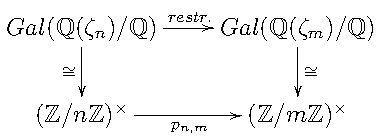
\includegraphics[width=0.3057\paperwidth]{images/L1-p006-diagram.pdf}\end{figure}
其中$p_{n,m}$把$[a]$映到$a\bmod m$。
\end{note}
\sourcepage{7}
对任意正整数$m$，定义$\varphi(m)$为$1$到$m$之间与$m$互素的整数个数。于是
\[|\Gal(\Q(\zeta_m)/\Q)|=[\Q(\zeta_m):\Q]=|(\Z/m\Z)^\times|=\varphi(m).\]
在经典数论中，算术函数$\varphi$称为\textbf{Euler函数}，并有如下结论。\idx{Euler函数}
\originalnumber{4}
\begin{theorem}\label{L1S2O4}
若$n=p_1^{a_1}\cdots p_l^{a_l}$，其中$p_1,\ldots,p_l$是$\Z$中互不相同的素数，则
\[\varphi(n)=n\left(1-\frac1{p_1}\right)\cdots\left(1-\frac1{p_l}\right).\]
\end{theorem}
\eref{定理}{L1S2O4}的证明从略，本讲末尾将给出参考文献。
\originalnumber{5}
\begin{corollary}\label{L1S2O5}
设$m,n$为两个互素的正整数，则$\Q(\zeta_n,\zeta_m)=\Q(\zeta_{mn})$。此外，$\Q(\zeta_m)\cap\Q(\zeta_n)=\Q$，因而由\eref{命题}{L1S1O4}，
\[\Gal(\Q(\zeta_{mn})/\Q)\cong\Gal(\Q(\zeta_m)/\Q)\times\Gal(\Q(\zeta_n)/\Q).\]
\end{corollary}
\begin{proof}
由$\zeta_{mn}^{m}=\zeta_n$和$\zeta_{mn}^{n}=\zeta_m$，有$\Q(\zeta_m,\zeta_n)\subseteq\Q(\zeta_{mn})$。另一方面，因$(m,n)=1$，存在整数$u,v$使$vm+un=1$。于是$\zeta_n^v\zeta_m^u=\zeta_{mn}$，故$\Q(\zeta_{mn})\subseteq\Q(\zeta_m,\zeta_n)$。

为证明$\Q(\zeta_m)\cap\Q(\zeta_n)=\Q$，只需证明$[\Q(\zeta_m,\zeta_n):\Q]=[\Q(\zeta_m):\Q]\,[\Q(\zeta_n):\Q]$。
% [Tutor Note: 原书 p7 该恒等式右端误写作 $[\Q(\zeta_n):\Q]\cdot[\Q(\zeta_n):\Q]$（两次 $\zeta_n$）；译文按正确写法处理。]因此，证明$\varphi(mn)=\varphi(m)\varphi(n)$即可。写成$n=p_1^{a_1}\cdots p_l^{a_l}$、$m=p_{l+1}^{a_{l+1}}\cdots p_{l+t}^{a_{l+t}}$，其中$p_1,\ldots,p_{l+t}$互不相同；由\eref{定理}{L1S2O4}，
\[\varphi(mn)=mn\left(1-\frac1{p_1}\right)\cdots\left(1-\frac1{p_{l+t}}\right)=\varphi(m)\varphi(n).\]
\end{proof}
在介绍Kronecker--Weber定理之前，我们稍作离题，先给出下面这个关于有限阿贝尔Galois群的有趣结论。
\originalnumber{6}
\begin{theorem}\label{L1S2O6}
每个有限阿贝尔群都可以实现为$\Q$的某个阿贝尔扩张的Galois群。
\end{theorem}
\begin{proof}
每个有限阿贝尔群都同构于$\prod_{j=1}^s(\Z/m_j\Z)^{a_j}$，其中$m_j,a_j$为正整数，$m_j$两两不同。
\sourcepage{8}
不失一般性，还可假定$m_j$均为素数的幂。对每个$m_j$，先构造$a_j$个阿贝尔扩张$L_1(m_j),\ldots,L_{a_j}(m_j)$，其Galois群均为$\Z/m_j\Z$。把这些扩张排成一个序列，简记为$L_1,L_2,\ldots$，并要求
\[\left(\prod_{l=1}^{t}L_l\right)\cap L_{t+1}=\Q,\qquad 1\leq t<\sum_{j=1}^s a_j.\]
% [Tutor Note: 原书 p8 此处下界误写作 $1\leq t\leq\sum_j m_j$，与定理中 $m_j$ 的含义不符；译文按正确的 $\sum_j a_j$ 处理。]
这样，由\eref{命题}{L1S1O4}即得所需结论。

从$m_1$开始。选取素数$p_1$使$p_1\equiv1\pmod{m_1}$。于是$\Gal(\Q(\zeta_{p_1})/\Q)$是阶为$p_1-1$的循环群；由于$m_1\mid(p_1-1)$，它有一个阶为$m_1$的子群。
% [Tutor Note: 原书 p8 作 "has a subgroup of order m_1"，旧译误作「指数」；指数为 m_1 的子群对应的是 $\Z/((p_1-1)/m_1)\Z$ 的商，与构造不符。本轮改正。]由Galois理论，得到$\Q(\zeta_{p_1})/\Q$的一个阿贝尔子扩张$L_1(m_1)/\Q$，其Galois群为$\Z/m_1\Z$。为得到$L_2(m_1)$，再选取一个不同于$p_1$的素数$p_2$，满足$p_2\equiv1\pmod{m_1}$，并重复这一过程。由下面的Dirichlet定理，对任意正整数$m$，满足$p\equiv1\pmod m$的素数$p$都有无穷多个。最终得到互不相同的素数$p_1,p_2,\ldots$和阿贝尔扩张$L_1,L_2,\ldots$，其中$L_l\subseteq\Q(\zeta_{p_l})$。由于$\prod_{l=1}^tL_l$包含于$\Q(\zeta_{\prod_{l=1}^t p_l})$，由\eref{推论}{L1S2O5}，
\[\left(\prod_{l=1}^{t}L_l\right)\cap L_{t+1}=\Q,\qquad1\leq t<\sum_{j=1}^s a_j.\]
\end{proof}
\originalnumber{7}
\begin{theorem}{Dirichlet}\label{L1S2O7}\idx{Dirichlet定理}
若$a,b\in\Z$且$(a,b)=1$，$b\ne0$，
% [Tutor Note: 原书 p10 未声明 $b\neq0$，而 $b=0$ 时同余式无意义；译文补上。]则满足$p\equiv a\pmod b$的正素数$p$有无穷多个。
\end{theorem}
\eref{定理}{L1S2O7}的结论曾由Gauss提出猜想，直到1837年才由Dirichlet首次证明。Dirichlet的证明使用了Dirichlet $L$-级数。\znote{Dirichlet $L$-级数定义为 $L(s,\chi)=\sum_{n\geq1}\chi(n)n^{-s}$，其中 $\chi$ 是模 $b$ 的 Dirichlet 特征标；由 $L(1,\chi)\neq0$ 可推出等差数列 $\{a+kb\}$ 中素数无穷多，这就是 Dirichlet 定理的解析证明。它也是 Langlands 纲领中 $L$ 函数的最初原型（$F=\Q$、$n=1$ 的情形）。[来源：K. Ireland, M. Rosen, \textit{A Classical Introduction to Modern Number Theory}, Springer-Verlag New York, 1990, 第 16 章（本讲参考文献 [IM]）；并见 nLab "L-function"，\url{https://ncatlab.org/nlab/show/L-function}（Last revised 2024-07-07；2026-11-14 访问）。]}这里略去证明，稍后给出参考文献。

然而，一旦去掉阿贝尔条件，问题便远未解决。\znote{此即\textbf{逆 Galois 问题}（inverse Galois problem）：是否每个有限群都同构于 $\Q$ 的某个有限 Galois 扩张的 Galois 群？阿贝尔情形由 Kronecker--Weber 定理肯定（即本讲定理 9）；一般情形仍未解决。已知可解群情形成立（Shafarevich），$S_n$、$A_n$ 及大量其他群也已实现，但一般有限群情形是公开问题。[来源：nLab "inverse Galois problem"，\url{https://ncatlab.org/nlab/show/inverse+Galois+problem}（Last revised 2023-05-27；2026-11-14 访问）。]}
\originalnumber{8}
\begin{problem}[（逆Galois问题）]\label{L1S2O8}\idx{逆Galois问题}
每个有限群是否都能实现为$\Q$的某个有限Galois扩张的Galois群？
\end{problem}
分圆域都是$\Q$的阿贝尔扩张，但$\Q$的阿贝尔扩张未必本身就是分圆域，例如二次数域$\Q(\sqrt2)$。
\begin{exercise*}\label{L1S2EX}
证明：二次数域$\Q(\sqrt d)$为分圆域，当且仅当$d=-1$或$-3$。（提示：$[\Q(\sqrt d):\Q]=2$，而$\varphi(m)=2\iff m=3,4,6$。
% [Tutor Note: 原书 p8 习题提示作「$m=4$ 或 $6$」，漏了 $m=3$（$\varphi(3)=2$）；译文已补正。]）
\end{exercise*}
\sourcepage{9}
不过，每个有限阿贝尔扩张都是某个分圆域的子域，正如下面这个优美定理所述。
\originalnumber{9}
\begin{theorem}{Kronecker--Weber}\label{L1S2O9}\idx{Kronecker--Weber定理}
$\Q$的每个有限阿贝尔扩张都包含于一个分圆域。
\end{theorem}
由\eref{定理}{L1S2O9}可知，$\Q^{\mathrm{ab}}$是把所有单位根添加到$\Q$中得到的域；换言之，$\Q^{\mathrm{ab}}=\prod_{m\in\Z_{>0}}\Q(\zeta_m)$。此外，
\[
\Gal(\Q^{\mathrm{ab}}/\Q)\cong\varprojlim_m(\Z/m\Z)^\times
=\left\{(x_m)_{m>0}\in\prod_{m>0}(\Z/m\Z)^\times\ \middle|\ p_{n,m}(x_n)=x_m\text{，对所有 }m\mid n\right\}.
\]
\eref{定理}{L1S2O9}的证明留待以后。事实上，它是类域论定理的一个推论；我们将在接下来的一两讲中讨论类域论。现在说明如何由\eref{定理}{L1S2O9}得到$\Q^{\mathrm{ab}}$与$\Gal(\Q^{\mathrm{ab}}/\Q)$的上述具体描述。令$\widetilde{\Q}$为把所有单位根添加到$\Q$中得到的域。需要证明$\Q^{\mathrm{ab}}=\widetilde{\Q}$。

首先证明$\Q^{\mathrm{ab}}\subseteq\widetilde{\Q}$。对任意$\alpha\in\Q^{\mathrm{ab}}$，$\Q(\alpha)/\Q$是有限阿贝尔扩张，由\eref{定理}{L1S2O9}，存在$m$使$\Q(\alpha)\subseteq\Q(\zeta_m)$。因此每个$\alpha\in\Q^{\mathrm{ab}}$都属于$\widetilde{\Q}$，故$\Q^{\mathrm{ab}}\subseteq\widetilde{\Q}$。再定义群同态
\[\widetilde\theta:\varprojlim_m(\Z/m\Z)^\times\longrightarrow\Gal(\widetilde{\Q}/\Q),\]
把每个相容族$(x_m)_{m>0}$映到由$\sigma(\zeta_m)=\zeta_m^{x_m}$确定的自同构$\sigma$。容易看出$\widetilde\theta$是双射，因而$\Gal(\widetilde{\Q}/\Q)$为阿贝尔群，进而$\widetilde{\Q}=\Q^{\mathrm{ab}}$。

本讲最后，我们借助$p$进数的概念，更具体地描述$\Gal(\Q^{\mathrm{ab}}/\Q)$。回忆：对每个素数$p$，$p$进整数环$\Z_p$是$\Z$关于极大理想$p\Z$的完备化；$\Q_p$是$\Z_p$的分式域。$\Q_p$中的元素称为\textbf{$p$进数}。每个非零$p$进数可以写成形式级数\idx{p进数@$p$进数}\idx{p进整数@$p$进整数}
\[a_kp^k+a_{k+1}p^{k+1}+a_{k+2}p^{k+2}+\cdots,\]
其中$a_{k+j}$为满足$0\leq a_{k+j}\leq p-1$的整数，且$a_k\ne0$。上述数属于$\Z_p$当且仅当$k\geq0$；属于$\Z_p^\times$当且仅当$k=0$。
\sourcepage{10}
\originalnumber{10}
\begin{note}[L1S2O10]
注意，$\Z\subsetneq\Z_p\cap\Q=\{a/b\mid(a,b)=1,\ p\nmid b\}$。例如，$1/3$在$\Z_2$中可写为$1-2+2^2-2^3+\cdots$。不过，$\left(\bigcap_p\Z_p\right)\cap\Q=\Z$。
\end{note}
令$\widehat{\Z}:=\prod_p\Z_p$\znote{$\widehat{\Z}$ 称为 $\Z$ 的\textbf{射有限完备化}，同构于 $\varprojlim_n\Z/n\Z$；在乘积拓扑下 $\prod_p\Z_p$ 与投影极限拓扑一致，都是紧、全不连通的射有限环。一般地，任何有限生成 $\Z$-模都有射有限完备化。[来源：nLab "profinite group"，\url{https://ncatlab.org/nlab/show/profinite+group}（Last revised 2025-07-01；2026-11-14 访问）。]}。
\originalnumber{11}
\begin{theorem}\label{L1S2O11}
$\displaystyle\varprojlim_m(\Z/m\Z)^\times\cong\prod_p\Z_p^\times=:\widehat{\Z}^\times$。
\end{theorem}
\begin{proof}
由于
\[\begin{aligned}\Z_p&=\varprojlim_n\Z/p^n\Z\\&=\left\{(x_{p^m})_{m>0}\in\prod_{m>0}\Z/p^m\Z\ \middle|\ \begin{array}{l}p_{p^n,p^m}(x_{p^n})=x_{p^m},\\\text{对所有 }m<n\end{array}\right\},\end{aligned}\]
$\widehat{\Z}$的每个元素都给出一个族\[\{x_{p^n}\}_{p\text{ 为素数},\,n>0}.\]只需证明：对每个这样的族，存在唯一的元素\[(x_m)\in\varprojlim_m\Z/m\Z,\]使$\{x_{p^n}\}$为它的子族。

为此，只需证明：对任意整数$\widetilde x_{p_1^{a_1}},\ldots,\widetilde x_{p_s^{a_s}}$，存在一个整数\[\widetilde x_{p_1^{a_1}\cdots p_s^{a_s}},\]在模$p_1^{a_1}\cdots p_s^{a_s}$的意义下唯一，满足
\[\widetilde x_{p_1^{a_1}\cdots p_s^{a_s}}\equiv\widetilde x_{p_j^{a_j}}\pmod{p_j^{a_j}},\qquad j=1,\ldots,s.\]
这由中国剩余定理得到，证明完毕。
\end{proof}
\lref{L2}将讨论Frobenius自同构与类域论。
\needspace{5\baselineskip}\section{第1讲参考文献}\label{L1S3}
\needspace{4\baselineskip}关于Galois理论：
\begin{references}\refitem{L1refL}{L} Serge Lang, \textit{Algebra}, Graduate Texts in Mathematics, Chapter VI (exercise 43 for Krull topology).\end{references}
\needspace{4\baselineskip}关于算术函数：
\begin{references}\refitem{L1refIM2}{IM} Kenneth Ireland and Michael Rosen, \textit{A Classical Introduction to Modern Number Theory}, Springer-Verlag New York, Inc. in 1990, Chapter 2.\end{references}
\needspace{4\baselineskip}关于Dirichlet定理：
\begin{references}\refitem{L1refIM16}{IM} Kenneth Ireland and Michael Rosen, \textit{A Classical Introduction to Modern Number Theory}, Springer-Verlag New York, Inc. in 1990, Chapter 16.\end{references}

\chapter{Frobenius自同构与类域论}\label{L2}
\lecturedate{2020/02/19}
\sourcepage{11}
我们已经描述了$\Q^{\mathrm{ab}}$和$\Gal(\Q^{\mathrm{ab}}/\Q)$。本讲研究任意代数数域$F$的阿贝尔扩张$L/F$。我们将利用类域论证明Kronecker--Weber定理，并介绍分类定理：阿贝尔扩张$L/F$可以由$F$的某些理想类群\znote{理想类群 $\mathrm{Cl}(F)=I_F/P_F$ 是分式理想群模去主分式理想群，其阶 $h_F$ 称为类数，数域的类数有限。它衡量 $\OO_F$ 偏离唯一分解的程度：$h_F=1$ 当且仅当 $\OO_F$ 是唯一分解整环；非平凡类群的存在正是类域论要处理的现象：例如 $\mathrm{Cl}(\Q)=1$，而 $\OO_{\Q(\sqrt{-5})}$ 的类数为 $2$，这对应 $2\cdot3=(1+\sqrt{-5})(1-\sqrt{-5})$ 给出的两种本质不同的分解。[来源：nLab "ideal class group"，\url{https://ncatlab.org/nlab/show/ideal+class+group}（Last revised 2018-05-11；2026-11-14 访问）。]}来参数化。
\section{代数数论预备知识}\label{L2S1}
按照定义，代数数域$F$是$\Q$的有限扩张。记$\OO_F$为$F$中的代数整数环\znote{$\OO_F$ 是 $F$ 的唯一极大序：任何由 $F$ 中代数整数构成的环都含于它。常见误解是把它当作唯一分解整环——$\OO_{\Q(\sqrt{-5})}=\Z[\sqrt{-5}]$ 中 $6=2\cdot3=(1+\sqrt{-5})(1-\sqrt{-5})$ 就是经典反例。它之所以仍是开展数论的良好舞台，是因为它是 Dedekind 整环：元素未必唯一分解，但理想一定唯一分解。[来源：Neukirch, \textit{Algebraic Number Theory}, Grundlehren der mathematischen Wissenschaften 322, 第 I 章 §8（本讲参考文献）。]}（换言之，$\OO_F$是$\Z$在$F$中的整闭包）。一般而言，$\OO_F$不是唯一分解整环，但它是Dedekind整环。设$L/F$为有限扩张，$D$为$\OO_F$在$L$中的整闭包。于是有以下性质。\idx{代数整数环}\idx{Dedekind整环}
\begin{property}
$D$是Dedekind整环，因此$D$中每个非零真理想都能唯一写成素理想的乘积。
\end{property}
\begin{definition*}{分歧指数与剩余次数}\idx{分歧指数}\idx{剩余次数}
$\OO_F$的每个非零素理想$\p$都满足$\p D\ne D$，因此有分解
\[\p D=\Pp_1^{e_1}\cdots\Pp_r^{e_r},\]
其中$\Pp_1,\ldots,\Pp_r$是$D$中满足$\Pp_j\cap\OO_F=\p$的素理想。$e_j$称为$\Pp_j$在$\p$上的\textbf{分歧指数}\znote{分歧指数 $e_j$ 是 $\p$ 在 $\Pp_j$ 中的重数，即 $e_j=v_{\Pp_j}(\p D)$，由 $\Pp_j^{e_j}\parallel\p D$ 刻画；它计量 $\p$ 在 $\Pp_j$ 处「重复」了多少次，$e_j>1$ 就是分歧的定量含义。易错之处在于：$e_j$ 依赖于 $\Pp_j$，同一 $\p$ 上方的不同素理想可以有不同分歧指数；但在 $L/F$ 为 Galois 时它们全都相等。[来源：Neukirch, \textit{Algebraic Number Theory}, Grundlehren der mathematischen Wissenschaften 322, 第 I 章 §8（本讲参考文献）。]}。
\sourcepage{12}
此外，$\OO_F/\p$与$D/\Pp_j$都是有限域\znote{$\OO_F/\p$ 称为 $\p$ 的\textbf{剩余域}（residue field），常记作 $\kappa(\p)$；$D/\Pp_j$ 是 $\Pp_j$ 的剩余域。二者都是有限域，而 $f_j=[\kappa(\Pp_j):\kappa(\p)]$ 是剩余域扩张的次数——这正是「剩余次数」一名的由来。剩余域之所以重要，是因为它与分歧指数 $e_j$ 一起完整刻画了 $\p$ 在 $\Pp_j$ 处的分解行为。[来源：Neukirch, \textit{Algebraic Number Theory}, Grundlehren der mathematischen Wissenschaften 322, 第 I 章 §8（本讲参考文献）。]}；域扩张的次数$f_j:=[D/\Pp_j:\OO_F/\p]$称为$\Pp_j$在$\p$上的\textbf{剩余次数}。
\end{definition*}
\begin{property}沿用上述记号，有$\displaystyle\sum_{j=1}^r e_jf_j=[L:F]$。\end{property}
\begin{definition*}{分裂与分歧}\idx{完全分裂}\idx{非分歧}\idx{全分歧}
仍用上述记号。若对$j=1,\ldots,r$都有$e_j=f_j=1$，就称素理想$\p$\textbf{完全分裂}\znote{「完全分裂」是分歧行为的极端情形：$\p D$ 分解为 $[L:F]$ 个互不相同的一次素理想，即 $e_j=f_j=1$ 对一切 $j$ 成立。等价的说法是 $\operatorname{Fr}[\p]=1$：完全分裂与否，取决于 Frobenius 元素是否平凡。原型例子是分圆域 $\Q(\zeta_m)/\Q$：$p\nmid m$ 时 $p$ 完全分裂当且仅当 $p\equiv1\pmod m$，即 $p$ 的 Frobenius 在 $(\Z/m\Z)^\times$ 中为 $1$。[来源：Neukirch, \textit{Algebraic Number Theory}, Grundlehren der mathematischen Wissenschaften 322, 第 I 章 §9（本讲参考文献）。]}；此时$r=n=[L:F]$。若$e_j=1$，就称$\Pp_j$在$\OO_F$上\textbf{非分歧}；否则称它\textbf{分歧}。若$\Pp_j$分歧且$f_j=1$，就称它\textbf{全分歧}。若所有$\Pp_j$都非分歧，就称$\p$非分歧；否则称$\p$分歧。
\end{definition*}
\begin{definition*}{非分歧扩张}
若$\OO_F$的所有非零素理想在$L$中都非分歧，就称扩张$L/F$\textbf{非分歧}。
\end{definition*}
\begin{property}在$L$中分歧的$\OO_F$的素理想只有有限多个。\end{property}
\begin{definition*}{上方的素理想}
若$\Pp\cap\OO_F=\p$，就说$\Pp$\textbf{位于$\p$上方}；这等价于$\Pp$出现在$\p D$的分解中。
\end{definition*}
进一步假定$L/F$是有限Galois扩张。仍用上述记号，有以下性质。
\begin{property}
若$\Pp\cap\OO_F=\p$，则对任意$\sigma\in\Gal(L/F)$，
\[\sigma\Pp\cap\OO_F=\sigma(\Pp\cap\OO_F)=\sigma(\p)=\p.\]
因此$\sigma\Pp$也位于$\p$上方。称$\sigma\Pp$（$\sigma\in\Gal(L/F)$）为与$\Pp$\textbf{共轭的素理想}。

由Hilbert分歧理论，$\Gal(L/F)$在$D$中所有位于$\p$上方的素理想组成的集合上传递作用，即这些素理想彼此共轭。
\end{property}
\begin{property}
因而，在素理想分解$\p D=\Pp_1^{e_1}\cdots\Pp_r^{e_r}$中，各剩余次数$f_j$相同：每个$\sigma\in\Gal(L/F)$都诱导同构$D/\Pp\xrightarrow{\sim}D/\sigma\Pp$（容易看出，对所有$\sigma$都有$\sigma(D)=D$）。各分歧指数也相同，因为
\[\sigma(\p D)=\p D=(\sigma\Pp_1)^{e_1}\cdots(\sigma\Pp_r)^{e_r}.\]
令$f_1=\cdots=f_r=f$、$e_1=\cdots=e_r=e$，则
\[efr=\sum_{j=1}^r e_jf_j=[L:F]=|\Gal(L/F)|.\]
\end{property}
\sourcepage{13}
\originalnumber{1}
\begin{example}\label{L2S1O1}
设$F=\Q$，$L=\Q(\zeta_m)$为分圆域。则：
\begin{enumerate}
\item 若$p$为不整除$m$的素数，则$(p)$在$L$中非分歧，其剩余次数$f$是满足$p^f\equiv1\pmod m$的最小正整数。
\item 若$m$为素数，则$(m)D=((1-\zeta_m))^{m-1}$，因此$(m)$全分歧，且$e=m-1$、$f=1$、$r=1$。
\end{enumerate}
\end{example}
\eref{例题}{L2S1O1}的第一个结论并不显然，读者可参阅\bref{L2refIM}{IM}。
\originalnumber{2}
\begin{example}\label{L2S1O2}
设$F=\Q$，$L=\Q(\zeta_4)=\Q(i)$，其中$i=\sqrt{-1}$，则$D=\Z[i]$。由于$[L:\Q]=2$，$(p)D$至多分解成两个素理想的乘积。设$p$为奇素数。若$(p)D$不是$D$中的素理想，则剩余次数$f$只能为$1$，因而$p\equiv1\pmod4$。此外，此时$p=(a+bi)(c+di)$，其中$a,b,c,d\in\Z$，且$(a,b)=(c,d)=1$。另一方面，$ad=-bc$；调整单位因子后可取$a=c$、$b=-d$，于是$p=a^2+b^2$。若$p\not\equiv1\pmod4$，则$f=2$，$(p)D$是$D$中的素理想，因而$p$不能写成两个整数的平方和。也就是说，对奇素数$p$，
% [Tutor Note: 原书 p13 作 "with a,b,c,c∈Z"，第四个变量应为 d（与后文 (c,d) 对应），译文按正确写法处理。]
\[\exists a,b\in\Z\text{ 使 }p=a^2+b^2\quad\iff\quad p\equiv1\pmod4.\]
\end{example}
\eref{例题}{L2S1O2}证明了下面这个Fermat定理。
\originalnumber{3}
\begin{theorem}{Fermat 1640，Euler 1754}\label{L2S1O3}
设$p$为奇素数，则$p$能写成两个整数的平方和$n^2+m^2$，当且仅当$p\equiv1\pmod4$。
\end{theorem}
\section{Frobenius自同构}\label{L2S2}
仍用$L,F,\OO_F,D$表示前述对象，并假定$L/F$是有限Galois扩张。设$\Pp$为$D$的素理想，$\p=\Pp\cap\OO_F$。
\originalnumber{1}
\begin{definition}{分解群}\label{L2S2O1}\idx{分解群}
子群$G_{\Pp}=\{\sigma\in\Gal(L/F)\mid\sigma\Pp=\Pp\}$称为$\Pp$在$F$上的\textbf{分解群}\znote{分解群 $G_{\Pp}$ 是 $\Pp$ 在 $\Gal(L/F)$ 作用下的稳定化子，其不动域称为 $\Pp$ 的分解域。由于 $G_{\Pp}$ 保持 $\Pp$，它自然作用在剩余域 $D/\Pp$ 上，并且 $G_{\Pp}$ 同构于局部扩张 $L_{\Pp}/F_{\p}$ 的 Galois 群——这是把整体问题局部化的第一步。群论上 $|G_{\Pp}|=e_{\Pp}f_{\Pp}$，而它在 $\Gal(L/F)$ 中的指数等于 $\p$ 上方素理想的个数 $r$。[来源：Neukirch, \textit{Algebraic Number Theory}, Grundlehren der mathematischen Wissenschaften 322, 第 I 章 §9（本讲参考文献）。]}。
\end{definition}
\sourcepage{14}
\originalnumber{2}
\begin{note}[L2S2O2]
注意，在分解$\p D=\Pp_1^e\cdots\Pp_r^e$中，$r=|\Gal(L/F)|/|G_{\Pp}|$。
\end{note}
\originalnumber{3}
\begin{proposition}\label{L2S2O3}
扩张$(D/\Pp)/(\OO_F/\p)$是Galois扩张，且自然同态$G_{\Pp}\longrightarrow\Gal((D/\Pp)/(\OO_F/\p))$是满射。
\end{proposition}
\eref{命题}{L2S2O3}的证明可见\bref{L2refN1}{N}。
\originalnumber{4}
\begin{definition}{惯性群}\label{L2S2O4}\idx{惯性群}
同态$G_{\Pp}\longrightarrow\Gal((D/\Pp)/(\OO_F/\p))$的核$I_{\Pp}\subseteq G_{\Pp}$称为$\Pp$在$F$上的\textbf{惯性群}\znote{惯性群 $I_{\Pp}$ 由在剩余域上作用平凡的 $\sigma\in G_{\Pp}$ 组成，即同态 $G_{\Pp}\to\Gal(\kappa(\Pp)/\kappa(\p))$ 的核。它的不动域是 $L/F$ 中在 $\Pp$ 处非分歧的最大子扩张；$I_{\Pp}=\{1\}$ 当且仅当 $\p$ 非分歧。非分歧时 $G_{\Pp}$ 循环，其生成元就是 Frobenius 元素，这解释了为何非分歧情形下 Frobenius 元素唯一。[来源：Neukirch, \textit{Algebraic Number Theory}, Grundlehren der mathematischen Wissenschaften 322, 第 I 章 §9（本讲参考文献）。]}。
\end{definition}
\originalnumber{5}
\begin{proposition}\label{L2S2O5}
惯性群$I_{\Pp}=\{1\}\iff\p$在$L$中非分歧。
\end{proposition}
\begin{proof}
$\p$非分歧$\iff$分歧指数$e=1\iff fr=|\Gal(L/F)|$。由于$f=|\Gal((D/\Pp)/(\OO_F/\p))|$，且$r=|\Gal(L/F)|/|G_{\Pp}|$，得到
\[|\Gal((D/\Pp)/(\OO_F/\p))|=|G_{\Pp}|\iff I_{\Pp}=\{1\}.\]
\end{proof}
由于$D/\Pp$和$\OO_F/\p$都是有限域，$\Gal((D/\Pp)/(\OO_F/\p))\cong\Gal(\F_{q^f}/\F_q)$，其中$q=p^n$，$p$为某个素数。因此，该Galois群是由Frobenius自同构$x\mapsto x^q$（$x\in\F_{q^f}$）生成的循环群$\Z/f\Z$。
\originalnumber{6}
\begin{definition}{Frobenius元素}\label{L2S2O6}\idx{Frobenius元素}
设$\p$在$L$中非分歧。定义$\Pp$处的\textbf{Frobenius元素}为$\Gal((D/\Pp)/(\OO_F/\p))\cong\Gal(\F_{q^f}/\F_q)$中Frobenius自同构在$G_{\Pp}$中的唯一原像，记作$\operatorname{Fr}[\Pp]$或$\left[\frac{L/F}{\Pp}\right]$。
\end{definition}
\originalnumber{7}
\begin{note}[L2S2O7]
\begin{enumerate}
\item 对任意$\sigma\in\Gal(L/F)$，有$G_{\sigma\Pp}=\sigma G_{\Pp}\sigma^{-1}$、$I_{\sigma\Pp}=\sigma I_{\Pp}\sigma^{-1}$。此外，$\operatorname{Fr}[\sigma\Pp]=\sigma\operatorname{Fr}[\Pp]\sigma^{-1}$。因此，$\operatorname{Fr}[\Pp]$在$\Gal(L/F)$中的共轭类只依赖于$\p$，记为$\operatorname{Fr}[\p]$或$\left[\frac{L/F}{\p}\right]$。
\item 由定义，对任意$x\in D$，有$\operatorname{Fr}[\Pp](x)\equiv x^q\pmod{\Pp}$。
% [Tutor Note: 原书 p14 作 Fr[P](x) ≡ x^f (mod P)，其中 f 为剩余次数；Frobenius 自同构应为 x↦x^q（q=|O_F/p|），译文按正确写法处理。]
\end{enumerate}
\end{note}
\section{类域论}\label{L2S3}\idx{类域论}
现在介绍类域论，它的目标是描述数域的阿贝尔扩张。这是一个相当广泛的主题，因此这里只能作非常简短的介绍。最初，\textbf{类域}$L/F$的定义要求分式理想的同余类群满足某个条件；
\sourcepage{15}
Takagi在1920年前后证明，这等价于$L/F$为有限阿贝尔扩张。仍沿用$L,F,\OO_F,D$的记号，并假定$L/F$有限阿贝尔。整体类域论可由局部类域论推出，在这种处理方法中需要用到阿代尔与伊代尔。本节则暂不使用这些概念，而通过Artin映射建立阿贝尔扩张$L/F$与某些理想类群之间的对应。不过，要完成主要定理的证明，仍须转向局部观点。

设$I_F$为$F$的分式理想群。对$\OO_F$中素理想的一个有限集$S$，定义$I_F^S$为由不属于$S$的素理想生成的$I_F$的子群。于是每个$\mathfrak{a}\in I_F^S$都有唯一分解
\[\mathfrak{a}=\p_1^{n_1}\cdots\p_s^{n_s},\qquad\p_j\notin S,\quad n_j\in\Z.\]
设$S$是包含所有在$L$中分歧的素理想的有限集（这些素理想只有有限多个）。\textbf{Artin映射}\znote{Artin 映射又称\textbf{互反映射}（reciprocity map）：它在每个 $\p\notin S$ 处取 Frobenius 元素 $\operatorname{Fr}[\p]$，再按乘法延拓到 $I_F^S$。称为「互反」，是因为把素理想送到 Frobenius 元素的这条对应正是二次互反律的高次推广；Frobenius 元素的共轭类只依赖 $\p$，故在阿贝尔情形这是群中确定的元素，映射才能乘性延拓。[来源：Cassels--Fr\"ohlich, \textit{Algebraic Number Theory}, 第 VII 章（本讲参考文献）。]}$\psi_{L/F}$定义为同态\idx{Artin映射}
\[\psi_{L/F}:I_F^S\longrightarrow\Gal(L/F),\qquad\p_1^{n_1}\cdots\p_s^{n_s}\longmapsto\prod_{j=1}^s\operatorname{Fr}[\p_j]^{n_j}.\]
% [Tutor Note: 原书 p15 把 Artin 映射的定义域写作 I^S_K，但 K 未定义，应为 F；译文按 I^S_F 处理。]
注意，$\Gal(L/F)$为阿贝尔群，因此$\operatorname{Fr}[\p_j]$是这个群中的一个确定元素，而不仅是共轭类。
\originalnumber{1}
\begin{note}[L2S3O1]
对素理想$\p\notin S$，$\psi_{L/F}(\p)=1\iff\p$在$L$中完全分裂。这是因为$\operatorname{Fr}[\p]$的阶等于剩余次数$f$。
\end{note}
对任意有限扩张$K/F$，定义\textbf{范映射}$N_{K/F}:I_K\longrightarrow I_F$，使$N_{K/F}(\Pp)=\p^f$，其中$\p=\Pp\cap\OO_F$，$f$是$\Pp$在$\p$上的剩余次数。于是有以下命题。\idx{范映射}
\originalnumber{2}
\begin{proposition}\label{L2S3O2}
设$L/F$与$L'/F'$有限阿贝尔，且$L\subseteq L'$、$F\subseteq F'$。则下图交换：
\begin{figure}[H]\centering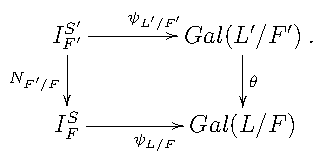
\includegraphics[width=0.2604\paperwidth]{images/L2-p015-diagram.pdf}\end{figure}
\sourcepage{16}
这里$S$是$\OO_F$中包含所有在$L'$中分歧的素理想的任意有限集，$S'$是$\OO_{F'}$中位于$S$中的素理想上方的所有素理想组成的集合。$\theta$是由以下复合给出的自然映射：
\[\Gal(L'/F')\longrightarrow\Gal(LF'/F')\longrightarrow\Gal(LF'/F)\longrightarrow\Gal(L/F).\]
\end{proposition}
\eref{命题}{L2S3O2}的证明直接，留给读者作为练习。
\originalnumber{3}
\begin{corollary}\label{L2S3O3}
Artin映射$\psi_{L/F}$为满射。
\end{corollary}
\begin{proof}
记$G'$为$\psi_{L/F}$的像。由Galois理论，存在中间域$F\subseteq K\subseteq L$，使$\Gal(K/F)=\Gal(L/F)/G'$且$\Gal(L/K)\cong G'$。因此，由\eref{命题}{L2S3O2}和\eref{笔记}{L2S3O1}，$F$中除有限多个以外的所有素理想都在$K$中完全分裂。由下面的命题，$K=F$。
\end{proof}
\originalnumber{4}
\begin{proposition}\label{L2S3O4}
设$K/F$为代数数域的有限扩张。如果$F$中除有限多个以外的所有素理想都在$K$中完全分裂，则$F=K$。（\bref{L2refN6}{N}第VI章第3节推论3.8。）
\end{proposition}
\originalnumber{5}
\begin{corollary}\label{L2S3O5}
$N_{L/F}(I_L^S)$包含于$\psi_{L/F}$的核。
\end{corollary}
\begin{proof}
在\eref{命题}{L2S3O2}中取$L'=L=F'$即可。
\end{proof}
回忆，$F$的无穷素位就是$F$的阿基米德素位，它与共轭嵌入对$(\iota,\overline\iota:F\hookrightarrow\C)$一一对应。若一个无穷素位$\infty$对应于$\iota_\infty=\overline\iota_\infty:F\hookrightarrow\R$，则称它为实素位；否则称为复素位。\znote{素位（place）是域上绝对值的等价类，等价指诱导同一拓扑。对代数数域 $F$，非阿基米德素位一一对应 $\OO_F$ 的非零素理想，阿基米德素位一一对应 $F\hookrightarrow\C$ 的嵌入的共轭类：实嵌入给出实素位，共轭嵌入对给出复素位。引进素位是为了让分歧、范数与 $L$ 函数在有限处与无穷处获得统一表述。[来源：nLab "place"，\url{https://ncatlab.org/nlab/show/place}（Last revised 2015-12-17；2026-11-14 访问）。]}\idx{无穷素位}

Artin互反律把$\ker\psi_{L/F}$描述为一个模$\mathfrak{m}$的同余子群。首先，定义$F$的一个\textbf{模}为形式乘积\idx{模（类域论）}
\[\mathfrak{m}=\prod_{\p}\p^{n(\p)},\]
其中$\p$遍历$F$的所有素位（包括无穷素位）。指数$n(\p)$为非负整数，只有有限多个为正；此外，若$\infty$为实素位，$n(\infty)$只能是$0$或$1$；若为复素位，则$n(\infty)=0$。
\sourcepage{17}
若$n(\p)>0$，就说素位$\p$整除$\mathfrak{m}$。记$I_F^{\mathfrak{m}}=I_F^S$，其中$S$为所有整除$\mathfrak{m}$的有限素位组成的集合。\par\needspace{5\baselineskip}定义
\[
F_{\mathfrak{m},1}=\left\{0\ne a\in F\ \middle|\ \begin{array}{l}\ord_{\p}(a-1)\geq n(\p)\text{，对所有有限素位 }\p\mid\mathfrak{m},\\\iota_\infty(a)>0\text{，对所有 }\infty\mid\mathfrak{m}\end{array}\right\}.
\]
$F_{\mathfrak{m},1}$的每个元素都给出一个$F$的主分式理想，因此有映射$i:F_{\mathfrak{m},1}\longrightarrow I_F$，其像包含于$I_F^{\mathfrak{m}}$。商群
\[C_{\mathfrak{m}}:=I_F^{\mathfrak{m}}/i(F_{\mathfrak{m},1})\]
称为\textbf{模$\mathfrak{m}$的射线类群}\znote{射线类群是理想类群的同余推广：$C_{\mathfrak{m}}=I_F^{\mathfrak{m}}/i(F_{\mathfrak{m},1})$ 把主理想换成由满足 $a\equiv1\pmod{\mathfrak{m}}$（在实素位处还要求 $a>0$）的元素生成的主理想。$\mathfrak{m}=1$ 时它退回通常的理想类群；模越大，$C_{\mathfrak{m}}$ 越大，而它恰参数化模 $\mathfrak{m}$ 的射线类域。注意 $i(F_{\mathfrak{m},1})$ 由主理想构成，故 $C_{\mathfrak{m}}$ 仍是「理想模主理想」型的商群，只是分子分母都加上了同余限制。[来源：Neukirch, \textit{Algebraic Number Theory}, Grundlehren der mathematischen Wissenschaften 322, 第 VI 章（本讲参考文献）。]}\idx{射线类群}
\originalnumber{6}
\begin{note}[L2S3O6]
若$\mathfrak{m}=1$，即所有指数$n(\p)$都为零，则$C_{\mathfrak{m}}$就是$F$的通常的类群，即分式理想群对主理想群取商所得的群。
\end{note}
\originalnumber{7}
\begin{theorem}{互反律}\label{L2S3O7}\idx{Artin互反律}
设$L$为$F$的有限阿贝尔扩张。则存在一个被所有在$L$中分歧的素理想整除的模$\mathfrak{m}$，使
\[\ker\psi_{L/F}=N_{L/F}(I_L^{\mathfrak{m}})\,i(F_{\mathfrak{m},1}).\]
换言之，$\Gal(L/F)\cong I_F^{\mathfrak{m}}/\bigl(N_{L/F}(I_L^{\mathfrak{m}})\,i(F_{\mathfrak{m},1})\bigr)$。
\end{theorem}
\originalnumber{8}
\begin{note}[L2S3O8]
Artin互反律有时写成表面上不同的形式，例如使用解析性质来表述，但它们本质上相同。
\end{note}
\originalnumber{9}
\begin{theorem}{存在唯一性定理}\label{L2S3O9}\idx{射线类域}
对$F$的任意模$\mathfrak{m}$，存在一个在同构意义下唯一的域$L_{\mathfrak{m}}$，称为\textbf{模$\mathfrak{m}$的射线类域}，使Artin映射定义同构$C_{\mathfrak{m}}\longrightarrow\Gal(L_{\mathfrak{m}}/F)$。
\end{theorem}
注意，$C_{\mathfrak{m}}$为阿贝尔群，故$L_{\mathfrak{m}}/F$是阿贝尔扩张。
\originalnumber{10}
\begin{corollary}{分类定理}\label{L2S3O10}
\begin{enumerate}
\item 设$H$为模$\mathfrak{m}$的同余子群，即$i(F_{\mathfrak{m},1})\subseteq H\subseteq I_F^{\mathfrak{m}}$。则存在阿贝尔扩张$L/F$，使$H=N_{L/F}(I_L^{\mathfrak{m}})\,i(F_{\mathfrak{m},1})$。
\item 每个有限阿贝尔扩张$L/F$都是某个射线类域的子扩张。
\end{enumerate}
\end{corollary}
现在可以把Kronecker--Weber定理作为\eref{推论}{L2S3O10}的特例来证明。
% [Tutor Note: 原书 p17 末作 "as a special case to Corollary 3.5"，按上下文应为推论 3.10（分类定理）；译文按正确编号处理。]
\sourcepage{18}
\begin{proof}[Kronecker--Weber定理的证明]
只需证明：对$\Q$的任意模$\mathfrak{m}$，模$\mathfrak{m}$的射线类域是某个分圆域的子扩张。注意，$\Q$只有一个无穷素位，记为$\infty$。若$\mathfrak{m}=m=p_1^{n_1}\cdots p_t^{n_t}$为正整数，则
\[I_{\Q}^{\mathfrak{m}}=\{(a/b)\mid(a,m)=(b,m)=1\},\]
\[\Q_{\mathfrak{m},1}=\{a/b\mid a,b\in\Z,\ a\equiv b\pmod m,\ (a,m)=1\},\]
并且
\[I_{\Q}^{\mathfrak{m}}\supseteq i(\Q_{\mathfrak{m},1})=\{(a/b)\mid a,b\in\Z_{>0},\ a\equiv\pm b\pmod m,\ (a,m)=1\}.\]
考察Artin映射$\psi_{\Q(\zeta_m)/\Q}:I_{\Q}^{\mathfrak{m}}\longrightarrow(\Z/m\Z)^\times$。对任意$p\nmid m$，由\eref{例题}{L2S1O1}，$\operatorname{Fr}[(p)]=[p]\in(\Z/m\Z)^\times$。因此
\[\ker\psi_{\Q(\zeta_m)/\Q}=\{(a/b)\mid a,b>0,\ (a,m)=(b,m)=1,\ a\equiv b\pmod m\}.\]
于是$\ker\psi_{\Q(\zeta_m)/\Q}\subseteq i(\Q_{\mathfrak{m},1})$，故模$\mathfrak{m}$的射线类域是$\Q(\zeta_m)$的子扩张，具体就是$\Q(\zeta_m+\zeta_m^{-1})$。

容易看出，$\Q(\zeta_m)$本身是模$\mathfrak{m}=m\cdot\infty$的射线类域。
\end{proof}
\needspace{5\baselineskip}\section{第2讲参考文献}\label{L2S4}
\needspace{4\baselineskip}关于Dedekind整环的扩张及Hilbert分歧理论：
\begin{references}\refitem{L2refN1}{N} J. Neukirch, \textit{Algebraic number theory}, Grundlehren der mathematischen Wissenschaften 322, Springer-Verlag Berlin Heidelberg GmbH, Chapter I \S8,\S9.\end{references}
\needspace{4\baselineskip}关于分圆域中的分歧：
\begin{references}\refitem{L2refIM}{IM} Kenneth Ireland and Michael Rosen, \textit{A Classical Introduction to Modern Number Theory}, Springer-Verlag New York, Inc. in 1990, Chapter 13 \S2.\end{references}
\needspace{4\baselineskip}关于整体类域论：
\begin{references}
\refitem{L2refN6}{N} J. Neukirch, \textit{Algebraic number theory}, Grundlehren der mathematischen Wissenschaften 322, Springer-Verlag Berlin Heidelberg GmbH, Chapter VI.
\refitem{L2refCF}{CF} J. W. S. Cassels and A. Fr\"ohlich, \textit{Algebraic Number Theory}, Proceedings of an instructional conference organized by the LMS, Chapter VII.
\end{references}

\chapter{局部整体原理、阿代尔与伊代尔}\label{L3}
\lecturedate{2020/02/24}
\sourcepage{19}
\section{局部整体原理}\label{L3S1}\idx{局部整体原理}
在定义阿代尔与伊代尔之前，先介绍局部整体原理。

数论关注的主要问题之一，是求多项式方程$P(x_1,\ldots,x_n)=0$的整数解，例如Fermat大定理所涉及的方程。不过，较容易判定的问题是是否存在“模$m$”的整数解，即
\[P(x_1,\ldots,x_n)\equiv0\pmod m.\]
此外，对任意素数$p$，对所有$k\in\Z_{>0}$，同余式$P(x_1,\ldots,x_n)\equiv0\pmod{p^k}$都有解，等价于$P(x_1,\ldots,x_n)=0$在$\Z_p$中可解。对于二次齐次多项式方程，有如下称为“局部整体原理”\znote{局部整体原理问的是：一个整体对象若在每个素位处都有局部解，能否由此断定它有整体解。Hasse--Minkowski 定理说二次型情形答案为「是」；但对次数不低于 $3$ 的方程一般不成立，局部可解只是必要条件，因此它是一类需要逐情形验证的现象，而非普遍方法。[来源：Neukirch, \textit{Algebraic Number Theory}, Grundlehren der mathematischen Wissenschaften 322, 第 VI 章（本讲参考文献）。]}的定理。
\originalnumber{1}
\begin{theorem}{Hasse--Minkowski}\label{L3S1O1}\idx{Hasse--Minkowski定理}
给定二次型$Q(x_1,\ldots,x_n)=\sum_{i,j=1}^n a_{ij}x_ix_j$，其中$(a_{ij})$为整数对称矩阵，且$\det(a_{ij})\ne0$。方程$Q(x_1,\ldots,x_n)=0$有非平凡整数解，当且仅当它有非平凡实数解，并对每个$p$都有非平凡$p$进解。
\end{theorem}
这里，$\R$是$\Q$关于阿基米德素位——绝对值$|\cdot|$——的完备化。把$\R$看作$\Q$在“无穷素位”处的完备化时，也记为$\Q_\infty$。\eref{定理}{L3S1O1}指出：$\Q$上的二次型有整体解，即$\Q$中的非平凡解，
\sourcepage{20}
当且仅当它在包括无穷素位在内的所有素位$p$处都有非平凡局部解。

局部整体原理与本课程并无很直接的关系，但它提示我们：如果把所有局部对象置于同等地位，整体对象或许能由其局部数据确定。设$F$为数域，$\OO_F$为其代数整数环。相对于在各素位处完备化所得的局部域$F_{\p}$，我们称$F$为整体域\znote{整体域指 $\Q$ 的有限扩张（数域）或 $\F_q(t)$ 的有限扩张（函数域）。与只看一个素位的局部域相对，整体域同时记住全部素位的算术；数域 $F$ 沿对角线嵌入 $\prod_{\p}F_{\p}$，其像离散，这使得「用全部局部数据刻画整体对象」成为可能。[来源：Neukirch, \textit{Algebraic Number Theory}, Grundlehren der mathematischen Wissenschaften 322, 第 VI 章（本讲参考文献）。]}。研究与$F$有关的对象时，可以为每个$F_{\p}$定义相应的局部对象，进行分析，并尝试寻找某种局部整体原理；尤其当局部对象可能更容易处理时，这样做很自然。

现在我们要描述$\Gal(F^{\mathrm{ab}}/F)$，因此考察$F$的所有素位处的$\Gal(F_{\p}^{\mathrm{ab}}/F_{\p})$。对域$K$，记$K^\times$为非零元素组成的乘法群。
\begin{enumerate}
\item 若$\p$为无穷素位，则$\overline F_{\p}=\C$，$F_{\p}=\R$或$\C$。因此$\Gal(\overline F_{\p}/F_{\p})$或为平凡群，或为二阶循环群。
\item 若$\p$为有限素位，则$F_{\p}$是带离散赋值的局部域\znote{局部域是「只用一个素位的显微镜看数域」所得的对象：完备化 $F_{\p}$ 保留 $\p$ 处的分歧与剩余域，却丢掉了其它素位的信息。非阿基米德局部域即 $\Q_p$ 或 $\F_q((t))$ 的有限扩张，其整数环是离散赋值环；阿基米德局部域只有 $\R$ 与 $\C$。[来源：Neukirch, \textit{Algebraic Number Theory}, Grundlehren der mathematischen Wissenschaften 322, 第 V 章（本讲参考文献）。]}。一般而言，$\Gal(\overline F_{\p}/F_{\p})$尚未被充分理解，但有限Galois扩张$L_{\Pp}/F_{\p}$的群$\Gal(L_{\Pp}/F_{\p})$有许多良好性质。此外，局部类域论给出$F_{\p}$的有限阿贝尔扩张与$F_{\p}^\times$的范数子群之间的一一对应。
\end{enumerate}
设$L/F$为有限Galois扩张，$D$为$\OO_F$在$L$中的整闭包。设$\Pp$为$L$中位于$F$的素位$\p$上方的素位。回忆，$\Pp$的分解群为
\[G_{\Pp}=\{\sigma\in\Gal(L/F)\mid\sigma\Pp=\Pp\}.\]
当$\p$为无穷素位时，它对应于$F$到$\R$或$\C$的嵌入（模去复共轭），$\Pp$则是这一嵌入到$L$的延拓。记此延拓为$\iota_{\Pp}$，则
\[G_{\Pp}=\{\sigma\in\Gal(L/F)\mid\iota_{\Pp}\circ\sigma=\iota_{\Pp}\text{ 或 }\overline\iota_{\Pp}\}.\]
% [Tutor Note: 原书 p20 的分解群条件只写 ι_P∘σ = ι_P；当 p 为实素位而 P 为复素位时，还应允许 ι_P∘σ 等于 ι_P 的共轭，译文按完整条件处理。]
我们知道$L_{\Pp}/F_{\p}$为Galois扩张，因此每个$\sigma\in G_{\Pp}$都诱导$L_{\Pp}$的一个$F_{\p}$-自同构，得到映射$i:G_{\Pp}\longrightarrow\Gal(L_{\Pp}/F_{\p})$。
\sourcepage{21}
\originalnumber{2}
\begin{proposition}\label{L3S1O2}
$i:G_{\Pp}\longrightarrow\Gal(L_{\Pp}/F_{\p})$为同构。
\end{proposition}
\begin{proof}
由于$L\subseteq L_{\Pp}$，$i$为单射。只需证明$|G_{\Pp}|=|\Gal(L_{\Pp}/F_{\p})|$。对于有限素位，设$\p D=\Pp_1^e\cdots\Pp_r^e$，其中$f=[D/\Pp_j:\OO_F/\p]$；由Hilbert分歧理论，$efr=[L:F]$（见\lref{L2}\sref{L2S1}）。另一方面，由于$\Gal(L/F)$在$\{\Pp_1,\ldots,\Pp_r\}$上传递作用，$r=|\Gal(L/F)|/|G_{\Pp}|$。因此
\[|\Gal(L_{\Pp}/F_{\p})|=[L_{\Pp}:F_{\p}]=ef=\frac{[L:F]}r=|G_{\Pp}|.\]
% [Tutor Note: 原书 p21 证明中把 [L:F] 写作 [L:K]，而本节 K 另指局部域，应为 [L:F]；译文按 [L:F] 处理。]
\end{proof}
由\eref{命题}{L3S1O2}，可把每个$\Gal(L_{\Pp}/F_{\p})$看成$\Gal(L/F)$的子群。
\section{局部类域论}\label{L3S2}\idx{局部类域论}
下面简要回顾局部类域论的一些结论。设$K$为局部域，$v_K$为规范化的离散赋值（即$v_K:K^\times\longrightarrow\Z$为满射）。设$\OO_K$为$K$的整数环，它是离散赋值环，有唯一的非零素理想$\p$。记剩余域为$k=\OO_K/\p$，则$k\cong\F_q$为有限域。
% [Tutor Note: 原书 p21 作 $v_K:K\to\Z$ 为满射；赋值在 $0$ 处无定义，定义域应为 $K^\times$，译文按 $v_K:K^\times\to\Z$ 处理。]
\begin{property}
设$E$为$K$的有限扩张，$R$为$\OO_K$在$E$中的整闭包。则$E$也是局部域，$R$为离散赋值环，$\Pp$为其唯一的非零素理想。记$E$的剩余域为$k_E=R/\Pp$，则$k_E$是$k$的有限扩张。
\end{property}
\begin{definition*}{局部非分歧扩张}
有$\p R=\Pp^e$及$e[k_E:k]=[E:K]=:n$。若$e=1$，称$E$在$K$上\textbf{非分歧}。
\end{definition*}
\begin{property}
若$E/K$非分歧，则$E/K$为Galois扩张$\iff k_E/k$为Galois扩张；在此情形下，$\Gal(E/K)\cong\Gal(k_E/k)$。因此，非分歧扩张都是阿贝尔扩张。
\end{property}
\sourcepage{22}
对有限Galois扩张$E/K$，定义范映射
\[N_{E/K}:E^\times\longrightarrow K^\times,\qquad\alpha\longmapsto\prod_{\sigma\in\Gal(E/K)}\sigma(\alpha).\]
\originalnumber{1}
\begin{theorem}\label{L3S2O1}
设$E/K$为有限Galois扩张。存在局部互反映射
\[\theta:K^\times/N_{E/K}(E^\times)\xrightarrow{\sim}\Gal(E/K)^{\mathrm{ab}},\]
且此映射为同构。
\end{theorem}
\eref{定理}{L3S2O1}的证明从略。这里只指出，若$E/K$非分歧，则$\Gal(E/K)\cong\Gal(k_E/k)$为阿贝尔群，由Frobenius元素$\mathcal F$生成；映射$\widetilde\theta(\alpha)=\mathcal F^{v_K(\alpha)}$（$\alpha\in K^\times$）诱导$\theta$。等式$\ker\widetilde\theta=N_{E/K}(E^\times)$由下面的命题得出。
\originalnumber{2}
\begin{proposition}\label{L3S2O2}
设$U_K$、$U_E$分别为$\OO_K$、$R$的单位群。若$E/K$非分歧，则$N_{E/K}(U_E)=U_K$。
\end{proposition}
\begin{exercise*}\label{L3S2EX}
利用\eref{命题}{L3S2O2}，证明当$E/K$非分歧时，$\ker\widetilde\theta=N_{E/K}(E^\times)$。
\end{exercise*}
若子群$M\subseteq K^\times$可写成$M=N_{E/K}(E^\times)$，其中$E/K$为某个有限阿贝尔扩张，就称$M$为\textbf{范数子群}\znote{范数子群就是「能作为某个有限阿贝尔扩张的范数像」的乘法子群。局部类域论断言：$K^\times$ 的有限指数闭子群恰好都是范数子群。于是 $K$ 的有限阿贝尔扩张与这些子群一一对应，阿贝尔扩张的全部信息被编码进 $K^\times$ 的群论数据，这正是类域论的核心。[来源：Neukirch, \textit{Algebraic Number Theory}, Grundlehren der mathematischen Wissenschaften 322, 第 V 章（本讲参考文献）。]}。\idx{范数子群}
\originalnumber{3}
\begin{theorem}{Galois对应}\label{L3S2O3}
$K$的有限阿贝尔扩张与$K^\times$的范数子群之间存在一一对应。此外，
\[N_{E_1/K}(E_1^\times)\subseteq N_{E_2/K}(E_2^\times)\iff E_2\subseteq E_1.\]
\end{theorem}
\originalnumber{4}
\begin{note}[L3S2O4]
范数子群$M\subseteq K^\times$还有一个内在刻画：$M$为范数子群，当且仅当它是$K^\times$中有限指数的闭子群；这里$K^\times$赋予Krull 拓扑\idx{Krull拓扑}。
\end{note}
% [Tutor Note: 原书 p22 Remark 2.4 把局部域 $K$ 写作 $F_{\p}$，与该节记号不符；译文按 $K^\times$ 处理。]
\originalnumber{5}
\begin{note}[L3S2O5]
\eref{定理}{L3S2O1}也可包括阿基米德情形。若$K=\C$，没有需要证明的内容；若$K=\R$，唯一的非平凡有限阿贝尔扩张$\C$对应于子群$\R_{>0}\subseteq\R^\times$。
\end{note}
\section{阿代尔与伊代尔}\label{L3S3}\idx{阿代尔}\idx{伊代尔}
设$F$为整体域，$F_{\p}$为$F$关于素位$\p$（允许为无穷素位）的完备化。若$\p$有限，记其赋值环为$\OO_{\p}$。
\sourcepage{23}
对于无穷素位，取$\OO_{\p}=F_{\p}$，其中$F_{\p}=\R$或$\C$。记$F_{\p}$上的赋值为$v_{\p}$。
% [Tutor Note: 原书 p23 作「$\OO_{\p}=\R_{\ge0}$（当 $F_{\p}=\R$）」；$\R_{\ge0}$ 对加法不封闭、不是环，此处应为 $\OO_{\p}=F_{\p}=\R$，译文按正确写法处理。]

$F$的\textbf{阿代尔环}$\A_F$\znote{阿代尔环把 $F$ 在所有素位处的完备化同时收进一个环，使「对所有素位同时成立」的陈述有统一载体。对角嵌入 $F\hookrightarrow\A_F$ 把数域的元素变成阿代尔。整体不变量（伊代尔类群、自守形式、$L$ 函数）都定义在 $\A_F$ 或其商上，这是 Langlands 纲领的技术起点。[来源：Cassels--Fr\"ohlich, \textit{Algebraic Number Theory}, 第 II 章（本讲参考文献）。]}是无限直积$\prod_{\p}F_{\p}$的子环，由所有满足$\alpha_{\p}\in F_{\p}$、且除有限多个$\p$外均有$\alpha_{\p}\in\OO_{\p}$的元素$\alpha=(\alpha_{\p})_{\p}$组成；这里$\p$遍历$F$的所有素位，包括无穷素位。

$\A_F$中的加法、乘法逐分量定义。这种乘积称为各$F_{\p}$关于子环$\OO_{\p}\subseteq F_{\p}$的\textbf{限制直积}\znote{限制直积的拓扑比 $\prod_{\p}F_{\p}$ 的直积拓扑更细：$\prod_{\p}\OO_{\p}$ 在限制直积拓扑下是开集，在子空间拓扑下却不是。原因是直积拓扑的每个基本开集只允许有限多个分量异于 $F_{\p}$。这一差别使 $\A_F$ 局部紧，而无限直积不局部紧；讨论收敛时必须用限制直积拓扑。[来源：Cassels--Fr\"ohlich, \textit{Algebraic Number Theory}, 第 II 章（本讲参考文献）。]}。各分量的拓扑赋予$\A_F$限制直积拓扑，使其成为拓扑环，加法与乘法连续。$\A_F$还是局部紧的，因为各$F_{\p}$局部紧，且有限素位处的$\OO_{\p}$紧。\idx{限制直积}\idx{阿代尔环}

$F$的\textbf{伊代尔群}$\mathbb{I}_F$是阿代尔环中的单位群$\mathbb{I}_F=\A_F^\times$\znote{伊代尔群 $\mathbb{I}_F=\A_F^\times$ 由各分量都非零、且除有限多个素位外分量为单位的元素组成。换言之，它是 $\prod'_{\p}F_{\p}^\times$ 关于 $\OO_{\p}^\times$ 的限制直积。它把每个素位处的乘法信息一并携带；商掉主伊代尔 $F^\times$ 得到伊代尔类群，后者正是整体类域论与自守表示论工作的对象。[来源：Cassels--Fr\"ohlich, \textit{Algebraic Number Theory}, 第 II 章（本讲参考文献）。]}。换言之，它是各$F_{\p}^\times$关于$\OO_{\p}^\times$的限制直积。设$S$为素位的一个有限集合，则$\mathbb{I}_F^S$为$S$-伊代尔组成的子群，满足
\[\mathbb{I}_F^S=\prod_{\p\in S}F_{\p}^\times\times\prod_{\p\notin S}\OO_{\p}^\times.\]
各嵌入$F^\times\hookrightarrow F_{\p}^\times$诱导嵌入$F^\times\hookrightarrow\mathbb{I}_F$。注意，对每个$x\in F^\times$，满足$x\notin\OO_{\p}^\times$的$\p$只有有限多个。
\originalnumber{1}
\begin{definition}{伊代尔类群}\label{L3S3O1}\idx{伊代尔类群}
商群$\mathbb{C}_F:=\mathbb{I}_F/F^\times$称为$F$的\textbf{伊代尔类群}。
\end{definition}
$\mathbb{I}_F$赋予限制直积拓扑。在此拓扑下，$F^\times$是$\mathbb{I}_F$的离散子群。

回忆，在\lref{L2}中，我们用$I_F$表示$F$的分式理想群；$C_F:=C_1=I_F/i(F^\times)$则是理想类群。有满同态
\[(\ ):\mathbb{I}_F\longrightarrow I_F,\qquad\alpha\longmapsto(\alpha)=\prod_{\p\text{ 有限}}\p^{v_{\p}(\alpha_{\p})}.\]
\sourcepage{24}
映射$(\ )$的核为
\[\mathbb{I}_F^\infty=\prod_{\p\text{ 无穷}}F_{\p}^\times\times\prod_{\p\text{ 有限}}\OO_{\p}^\times.\]
因而有以下命题。
\originalnumber{2}
\begin{proposition}\label{L3S3O2}
映射$(\ )$诱导满射$\mathbb{C}_F\longrightarrow C_F$，其核为$\mathbb{I}_F^\infty F^\times/F^\times$。因此$C_F\cong\mathbb{I}_F/(\mathbb{I}_F^\infty F^\times)$。
\end{proposition}
对有限阿贝尔扩张$L/F$，结合\eref{命题}{L3S1O2}和\eref{定理}{L3S2O1}，可以定义整体互反映射$\theta:\mathbb{I}_F/N_{L/F}(\mathbb{I}_L)\longrightarrow\Gal(L/F)$。这里$N_{L/F}:\mathbb{I}_L\longrightarrow\mathbb{I}_F$定义为
\[N_{L/F}(\alpha^L)=\left(\prod_{\Pp\mid\p}N_{L_{\Pp}/F_{\p}}(\alpha^L_{\Pp})\right)_{\p}.\]
把每个$\Gal(L_{\Pp}/F_{\p})$看作$\Gal(L/F)$中的子群$G_{\Pp}=G_{\p}$，即可定义
\[\widetilde\theta:\mathbb{I}_F\longrightarrow\Gal(L/F),\qquad\widetilde\theta(\alpha)=\prod_{\p}\widetilde\theta_{\p}(\alpha_{\p}).\]
这个乘积有意义：对于在$L$中非分歧的$\p$，$\widetilde\theta_{\p}(\alpha_{\p})=\operatorname{Fr}[\p]^{v_{\p}(\alpha_{\p})}$；分歧的$\p$只有有限多个，且除有限多个$\p$外均有$v_{\p}(\alpha_{\p})=0$。$\widetilde\theta$诱导映射$\theta$。但$\theta$本身不是同构；有如下同样称为Artin互反律的定理。
\originalnumber{3}
\begin{theorem}{Artin互反律}\label{L3S3O3}
$F^\times\subseteq\ker\widetilde\theta$。换言之，$\displaystyle\prod_{\p}\widetilde\theta_{\p}(x)=1$，对所有$x\in F^\times$成立。
\end{theorem}
由\eref{定理}{L3S3O3}，得到映射$\overline\theta:\mathbb{C}_F/N_{L/F}(\mathbb{C}_L)\longrightarrow\Gal(L/F)$。一个并不平凡的事实是，$\overline\theta$实际上是同构。由此可以用伊代尔类的范数群参数化$F$的所有有限阿贝尔扩张。
\originalnumber{4}
\begin{theorem}\label{L3S3O4}
\begin{enumerate}
\item $\Gal(L/F)\cong\mathbb{C}_F/N_{L/F}(\mathbb{C}_L)$。
% [Tutor Note: 原书 p24 定理 3.4(1) 作 Gal(L/K)，K 未定义，应为 Gal(L/F)；译文按 Gal(L/F) 处理。]
\item 映射$L\longmapsto N_{L/F}(\mathbb{C}_L)$给出$F$的有限阿贝尔扩张与$\mathbb{C}_F$中有限指数闭子群之间的一一对应。此外，
\[L_1\subseteq L_2\iff N_{L_1/F}(\mathbb{C}_{L_1})\supseteq N_{L_2/F}(\mathbb{C}_{L_2}).\]
\end{enumerate}
\end{theorem}
\sourcepage{25}
最后说明局部与整体互反映射的相容性。定义$\iota_{\p}:F_{\p}^\times\hookrightarrow\mathbb{C}_F$，把$a_{\p}$映到仅在$\p$分量为$a_{\p}$、其他分量全为$1$的伊代尔的类。于是有以下命题。
\originalnumber{5}
\begin{proposition}\label{L3S3O5}
设$L/F$为有限阿贝尔扩张，$\p$为$F$的一个素位（允许为无穷素位），$\Pp$为$L$中位于$\p$上方的素位。则下图交换：
\begin{figure}[H]\centering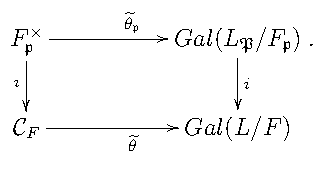
\includegraphics[width=0.2604\paperwidth]{images/L3-p025-diagram.pdf}\end{figure}
\end{proposition}
\eref{命题}{L3S3O5}表明，\eref{定理}{L3S3O4}中的同构$\overline\theta$满足某种刚性条件。
% [Tutor Note: 原书 p25 作「Theorem 3.3 中的同构 θ̄」，但 θ̄ 出现于 Theorem 3.4，Theorem 3.3 是 Artin 互反律；译文按定理 3.4 处理。]

\textbf{$n=1$时的Langlands纲领。}由无限Galois理论，
\begin{align*}
\Gal(F^{\mathrm{ab}}/F)&=\varprojlim_{L/F\text{ 有限阿贝尔}}\Gal(L/F)\\
&=\varprojlim_{N\text{ 为有限指数闭子群}}(\mathbb{C}_F/N).
\end{align*}
因此$\Gal(F^{\mathrm{ab}}/F)\cong G$，其中$G$为$\mathbb{C}_F$的连通分支群。

至此，我们完成了阿贝尔情形，即$n=1$时的Langlands纲领。对于一般$n$，Langlands纲领研究的不是Galois群$\Gal(\overline F/F)$本身，而是它的$n$维表示，即群同态$\sigma:\Gal(\overline F/F)\longrightarrow\GL_n$。它猜想存在如下的一一对应：
\[\left\{\begin{array}{c}\Gal(\overline F/F)\text{ 的}\\n\text{ 维表示}\end{array}\right\}\quad\overset{1\text{--}1}{\longleftrightarrow}\quad\left\{\begin{array}{c}\GL_n(\A_F)\text{ 的}\\\text{自守表示}\end{array}\right\}.\]
接下来的一两讲将定义自守表示，并考察$n=2$、$F=\Q$的非阿贝尔情形。
\needspace{5\baselineskip}\section{第3讲参考文献}\label{L3S4}
\needspace{4\baselineskip}关于局部类域论：
\sourcepage{26}
\begin{references}
\refitem{L3refN5}{N} J. Neukirch, \textit{Algebraic number theory}, Grundlehren der mathematischen Wissenschaften 322, Springer-Verlag Berlin Heidelberg GmbH, Chapter V.
\refitem{L3refCF6}{CF} J. W. S. Cassels and A. Fr\"ohlich, \textit{Algebraic Number Theory}, Proceedings of an instructional conference organized by the LMS, Chapter VI.
\end{references}
\needspace{4\baselineskip}关于阿代尔与伊代尔：
\begin{references}
\refitem{L3refN6}{N} J. Neukirch, \textit{Algebraic number theory}, Grundlehren der mathematischen Wissenschaften 322, Springer-Verlag Berlin Heidelberg GmbH, Chapter VI.
\refitem{L3refCF2}{CF} J. W. S. Cassels and A. Fr\"ohlich, \textit{Algebraic Number Theory}, Proceedings of an instructional conference organized by the LMS, Chapter II.
\end{references}
\needspace{4\baselineskip}关于伊代尔表述的Artin互反律：
\begin{references}
\refitem{L3refN6b}{N} J. Neukirch, \textit{Algebraic number theory}, Grundlehren der mathematischen Wissenschaften 322, Springer-Verlag Berlin Heidelberg GmbH, Chapter VI.
\refitem{L3refCF7}{CF} J. W. S. Cassels and A. Fr\"ohlich, \textit{Algebraic Number Theory}, Proceedings of an instructional conference organized by the LMS, Chapter VII.
\end{references}

\chapter{阿代尔群的自守表示I：一般定义}\label{L4}
\lecturedate{2020/02/26}
\sourcepage{27}
Langlands猜想断言，$n$维不可约Galois表示——即数域$F$的群$\Gal(\overline F/F)$的表示——与$\GL_n(\A_F)$的自守表示\znote{「自守」指函数在 $G(\Q)$ 左作用下的不变性（automorphy）。自守表示把这种不变性提升为 $G(\A)$ 的表示：它是带有整体不变性的一类表示，而非 $G(\A)$ 的任意表示。Galois 表示携带算术信息但缺少解析结构，Langlands 猜想断言两者是同一对象的两面。[来源：Bernstein--Gelbart, \textit{An introduction to the Langlands Program}, Birkh\"auser, 2004, 第 7 章（本讲参考文献）。]}之间存在一一对应。当$n=2$、$F=\Q$时，该猜想成立；粗略地说，在这一情形中，对应通过如下方式建立：
% [Tutor Note: 原书此处用语宽泛；就本书语境而言，已知成立的是 $n=1$ 的类域论情形。]
\begin{figure}[H]\centering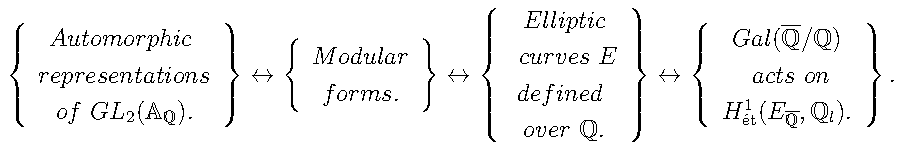
\includegraphics[width=0.7257\paperwidth]{images/L4-p027-correspondence.pdf}\end{figure}
记$\A_F^f$为$\A_F$的有限部分，即$\A_F$投影到$\prod_{\p\text{ 有限}}F_{\p}$所得的像。按照定义，$G(\A_{\Q})$的自守表示是$G(\Q)\backslash G(\A_{\Q})$上某个函数空间$\mathcal A(G)$的子商表示。严格地说，$\mathcal A(G)$并不承载整个$G(\R)$的作用；实际作用于它的是$G(\A_{\Q}^f)\times(K,\g)$，其中$K$为$G(\R)$的极大紧子群，$\g$是$G(\R)$的Lie代数。
% [Tutor Note: 原书 p27 作「$K$ is the maximal compact subgroup of $\A_{\Q}$」；$\A_{\Q}$ 是阿代尔环、没有紧子群这一说法，此处应为 $G(\R)$，译文按 $G(\R)$ 处理。]
\section{阿代尔环作为拓扑环的进一步性质}\label{L4S1}
设$F$为数域，$\p$为$F$的有限素位，$F_{\p}$为$F$在$\p$处完备化得到的局部域，并取规范化离散赋值$v_{\p}$。
\sourcepage{28}
定义绝对值$|x|_{\p}=q^{-v_{\p}(x)}$（$x\ne0$），并令$|0|_{\p}=0$；这里$\OO_{\p}/\p\cong\F_q$，$\OO_{\p}$为$F_{\p}$中的离散赋值环。
% [Tutor Note: 原书 p28 印作 $|x|_{\p}=q^{v_{\p}(x)}$，指数缺负号；乘积公式要求 $|x|_{\p}=q^{-v_{\p}(x)}$，译文按正确写法处理。]
$|\cdot|_{\p}$给出度量，从而在$F_{\p}$及$F_{\p}^\times$上给出拓扑。以下标准事实容易验证。
\begin{property}
\begin{itemize}
\item $F_{\p}$局部紧。
\item $\OO_{\p}$紧。
\item $F_{\p}$和$F_{\p}^\times$都是全不连通的，即非空连通子集只能是单点。
\end{itemize}
\end{property}
若$\p$为无穷素位，它对应于嵌入$\iota_{\p}:F\hookrightarrow\C$。实素位处定义$|x|_{\p}=|\iota_{\p}(x)|$，复素位处定义$|x|_{\p}=|\iota_{\p}(x)|^2$，其中右边为$\C$的通常绝对值。无穷素位处的$\OO_{\p}=F_{\p}$不紧，$F_{\p}$和$F_{\p}^\times$也不全不连通，但$F_{\p}$仍局部紧。

因为$F\subseteq F_{\p}$，所以对$X\in F^\times$，各处的$|X|_{\p}$均有定义。
\originalnumber{1}
\begin{theorem}\label{L4S1O1}\idx{乘积公式}
设$X\in F^\times$，则除至多有限多个$\p$外都有$|X|_{\p}=1$，且$\displaystyle\prod_{\p}|X|_{\p}=1$。
\end{theorem}
\originalnumber{2}
\begin{lemma}\label{L4S1O2}
设$X\in F^\times$，则除至多有限多个$\p$外都有$|X|_{\p}\leq1$。
\end{lemma}
\begin{proof}
$F$的无穷素位只有有限多个，因为$F/\Q$有限，而$\Q$只有一个无穷素位。因此只需考虑有限素位$\p$，此时$|\cdot|_{\p}$是非阿基米德绝对值。设$X\in F$，则$X$在$\Q$上是代数的，故
\[X^m+a_1X^{m-1}+\cdots+a_m=0,\qquad a_1,\ldots,a_m\in\Q.\]
于是
\[|X|_{\p}^m\leq\max\{|a_1|_{\p}|X|_{\p}^{m-1},\ldots,|a_m|_{\p}\}\leq\max\{1,|X|_{\p}^{m-1}\}\max_i|a_i|_{\p}.\]
固定的有理数$a_1,\ldots,a_m$在几乎所有有限素位处都满足$|a_i|_{\p}\leq1$；若此时$|X|_{\p}>1$，上述不等式便给出$|X|_{\p}^m\leq|X|_{\p}^{m-1}$，矛盾。因此$|X|_{\p}\leq1$。
\end{proof}
\sourcepage{29}
\begin{proof}[\eref{定理}{L4S1O1}的证明概要]
由\eref{引理}{L4S1O2}，对几乎所有$\p$，有$|X|_{\p}\leq1$和$|X^{-1}|_{\p}\leq1$，故$|X|_{\p}=1$。再利用规范化赋值在扩张中的性质，将乘积公式归结为$F=\Q$的情形；直接计算即得结论。
\end{proof}
可以定义群同态
\begin{equation}\tag{1.1}\label{L4eq11}
c:\mathbb{I}_F\longrightarrow\R_{>0},\qquad\alpha=(\alpha_{\p})_{\p}\longmapsto\prod_{\p}|\alpha_{\p}|_{\p}.
\end{equation}
\begin{exercise*}\label{L4S1EX1}
证明\eqref{L4eq11}中的$c$良定义，即对所有$\alpha\in\mathbb{I}_F$，右边的乘积都在$\R_{>0}$中有意义。
\end{exercise*}
由\eref{定理}{L4S1O1}，$F^\times\subseteq\ker c=:\mathbb{I}_F^1$。
\originalnumber{3}
\begin{theorem}{弱逼近定理}\label{L4S1O3}\idx{弱逼近定理}
设$|\cdot|_j$（$1\leq j\leq N$）为域$F$上有限个彼此不等价的非平凡绝对值。记$F_j$为集合$F$配上$|\cdot|_j$诱导的拓扑所得的拓扑空间。则$F$经对角嵌入所得的像$\Delta\subseteq\prod_{j=1}^N F_j$在$\prod_{j=1}^N F_j$中稠密。
\end{theorem}
\originalnumber{4}
\begin{note}[L4S1O4]
\eref{定理}{L4S1O3}等价于如下陈述：给定任意$x_j\in F$（$1\leq j\leq N$）和任意实数$\varepsilon>0$，存在$y\in F$，使$|x_j-y|_j<\varepsilon$，对$1\leq j\leq N$均成立。
\end{note}
\begin{proof}[\eref{定理}{L4S1O3}的证明概要]
只需找到$\xi_j\in F$（$j=1,\ldots,N$），使$|\xi_j|_j>1$，且当$k\ne j$时有$|\xi_j|_k<1$。对充分大的$r$，令
\[y:=\sum_{j=1}^N\frac{\xi_j^r}{1+\xi_j^r}x_j.\]
\sourcepage{30}
于是
\begin{align*}
|y-x_j|_j&=\left|\sum_{k\ne j}\frac{\xi_k^r}{1+\xi_k^r}x_k-\frac1{1+\xi_j^r}x_j\right|_j\\
&\leq\sum_{k\ne j}\frac{|\xi_k|_j^r}{|1+\xi_k^r|_j}|x_k|_j+\frac1{|1+\xi_j^r|_j}|x_j|_j.
\end{align*}
因$|\xi_k|_j<1$，当$r\to\infty$时，$\frac{|\xi_k|_j^r}{|1+\xi_k^r|_j}|x_k|_j\to0$。又因$|\xi_j|_j>1$，有$|1+\xi_j^r|_j\geq|\xi_j|_j^r-1$，故$\frac1{|1+\xi_j^r|_j}|x_j|_j\to0$。
\end{proof}
\originalnumber{5}
\begin{note}[L4S1O5]
\eref{定理}{L4S1O3}表明，对于$\prod_{j=1}^NF_j$的任意开子群$U$，有$\prod_{j=1}^NF_j=\Delta+U$。这是因为，对任意$x\in\prod_{j=1}^NF_j$，$x+U$为$x$的邻域，故存在$y\in(x+U)\cap\Delta$。因此$x=y-u$，其中$y\in\Delta$、$u\in U$。
\end{note}
设$L/F$为有限扩张，$D$为$\OO_F$在$L$中的整闭包。
\originalnumber{6}
\begin{lemma}\label{L4S1O6}
设$\omega_1,\ldots,\omega_n$为$L/F$的一组基。则对几乎所有$\p$，有
\[\omega_1\OO_{\p}\oplus\cdots\oplus\omega_n\OO_{\p}=D_{\Pp_1}\oplus\cdots\oplus D_{\Pp_r},\]
其中$\p D=\Pp_1\cdots\Pp_r$。
\end{lemma}
现在说明阿代尔环$\A_F$上的拓扑：取如下形式的集合为开集基，
\[\prod_{\p}U_{\p},\]
其中$U_{\p}$在$F_{\p}$中开，且对几乎所有$\p$有$U_{\p}=\OO_{\p}$。这一拓扑称为\textbf{限制直积拓扑}。伊代尔群$\mathbb{I}_F$上的限制直积拓扑类似定义。
\begin{exercise*}\label{L4S1EX2}
证明在限制直积拓扑下，\eqref{L4eq11}中的映射$c$连续。
\end{exercise*}
\originalnumber{7}
\begin{proposition}\label{L4S1O7}
作为拓扑环，有$\A_L\cong\A_F\otimes_F L\cong\A_{\Q}\otimes_{\Q} L$。这里，把$\A_F\otimes_F L$看作$\A_F\omega_1\oplus\cdots\oplus\A_F\omega_n$，由$\A_F$上的拓扑赋予它拓扑，其中$\omega_1,\ldots,\omega_n$为$L/F$的一组基。
\end{proposition}
\sourcepage{31}
\originalnumber{8}
\begin{theorem}\label{L4S1O8}
$F$在$\A_F$中离散，而商拓扑下的$\A_F/F$是紧的。这里把$\A_F$看作加法群，把$F$看作其子群。
\end{theorem}
\begin{proof}
由\eref{命题}{L4S1O7}，只需证明$F=\Q$的情形。定义
\[\A_{\Q}\supseteq U:=\prod_p\Z_p\times(-1,1).\]
则$U$是$\A_{\Q}$中包含$0\in\Q$的开集，且不含$\Q$中的其他元素。这是因为$\bigcap_p\Z_p\cap\Q=\Z$，而$\Z\cap(-1,1)=\{0\}$。因此$\Q$在$\A_{\Q}$中离散。

为证明$\A_{\Q}/\Q$紧，只需找到$\A_{\Q}$中的一个紧子集，其像覆盖$\A_{\Q}/\Q$。定义
\[W:=\prod_p\Z_p\times\left[-\frac12,\frac12\right].\]
如上所见，$W\cap\Q=\{0\}$，故$W\to\A_{\Q}/\Q$为单射。下面证明：对任意$\beta=(\beta_p)_p\times\beta_\infty\in\A_{\Q}$，存在$b\in\Q$，使每个$p$都满足$\beta_p-b\in\Z_p$，且$\beta_\infty-b\in[-1/2,1/2]$。写$\beta_p=\sum_j a_p^jp^j$，并定义$\gamma_p=\sum_{j<0}a_p^jp^j$；于是$\beta_p-\gamma_p\in\Z_p$，且除有限多个$p$外均有$\gamma_p=0$。令$\gamma=\sum_p\gamma_p$。由于当$p'\ne p$时$p^j\in\Z_{p'}$，对所有$p$都有$\beta_p-\gamma\in\Z_p$。最后取$s\in\Z$，使$\beta_\infty-\gamma-s\in[-1/2,1/2]$，再令$b=\gamma+s$，即得结论。
\end{proof}
类似地，$F^\times$在$\mathbb{I}_F$中离散。不过，作为乘法群的商，$\mathbb{I}_F/F^\times$不再紧。仍有如下结论。
\originalnumber{9}
\begin{theorem}\label{L4S1O9}
$\mathbb{I}_F^1/F^\times$在商拓扑下是紧的。
\end{theorem}
\eref{定理}{L4S1O9}的证明与\eref{定理}{L4S1O8}的证明类似。

对一个有限素位集$S$，记$\A_F^S$为各$F_{\p}$（$\p\notin S$）关于子环$\OO_{\p}\subseteq F_{\p}$的限制直积。（这个记号与\lref{L3}中定义的$\mathbb{I}_F^S$的意义不同。）本节最后介绍如下定理。
\sourcepage{32}
\originalnumber{10}
\begin{theorem}{强逼近定理}\label{L4S1O10}\idx{强逼近定理}
若$S$非空，则$F$在$\A_F^S$中稠密。
\end{theorem}
\originalnumber{11}
\begin{note}[L4S1O11]
令$F_S:=\prod_{\p\in S}F_{\p}$。由\eref{定理}{L4S1O10}，对$\A_F^S$的任意开子群$U^S$，有$\A_F=F+F_S+U^S$。例如，$\A_{\Q}=\Q+\R+\widehat{\Z}$，且$\Q\backslash\A_{\Q}/\widehat{\Z}=\R/(\widehat{\Z}\cap\Q)=\R/\Z$。
\end{note}
\section{阿代尔群}\label{L4S2}\idx{阿代尔群}
本节取$F=\Q$，以$\A$、$\A^f$分别简记$\A_{\Q}$、$\A_{\Q}^f$。设$G$为$\Q$上定义的线性代数群，例如$\GL_n$或$\SL_n$。令$G(\A)$为$G$的阿代尔点群，即$G(\A)=G(\A^f)\times G(\R)$，其中$G(\A^f)$为各$G(\Q_p)$关于$G(\Z_p)$的限制直积。称$G(\A)$为$G$的\textbf{阿代尔群}。

定义$K=\prod_p G(\Z_p)\times O$，其中$O$为$G(\R)$的极大紧子群。特别地，若$G=\GL_n$，可取$O=\operatorname O(n)$，即实正交矩阵群。在这些标准情形中，$K$是$G(\A)$的极大紧子群。以下固定这个$K$。
% [Tutor Note: 原书 p32 作「$K$ is a maximal compact subgroup of $G(\R)$」；$K$ 含有限部分 $\prod_p G(\Z_p)$，是 $G(\A)$ 的极大紧子群，译文按 $G(\A)$ 处理。]

对于$G(\Q)\subseteq G(\A)$，有如下性质。
\begin{property}
\begin{itemize}
\item $G(\Q)$在$G(\A)$中离散。
\item $G(\Q)\backslash G(\A)$一般不紧，但它有基本域。
\item 若$G$半单，则$G(\Q)\backslash G(\A)$的体积有限。
\end{itemize}
\end{property}
还有如下与\eref{定理}{L4S1O10}相对应的定理。
\originalnumber{1}
\begin{theorem}{$G$的强逼近定理}\label{L4S2O1}
设$G$为单连通半单群，$S$为$\Q$的有限素位集（可包括无穷素位），并要求$G$的每个几乎单因子在$\Q_S:=\prod_{p\in S}\Q_p$上的点群都不紧。则$G(\Q)$在$G(\A^S)$中稠密。
\end{theorem}
% [Tutor Note: 原书 p32 定理 2.1 的条件只写「$G(\Q_S)$ 不紧」；严格的强逼近定理要求 $G$ 的每个几乎单因子在 $\Q_S$ 上的点群都不紧，译文按后者处理。]
\sourcepage{33}
因此，对$G(\A^S)$的任意开子群$U^S$，有$G(\A)=G(\Q)\,G(\Q_S)\,U^S$。进一步设$U^S$紧，定义$\Gamma:=G(\Q)\cap(G(\Q_S)\,U^S)$，则
\[G(\Q)\backslash G(\A)/U^S\cong\Gamma\backslash G(\Q_S),\]
其中右边的$\Gamma$通过投影$G(\A)\longrightarrow G(\Q_S)$看成$G(\Q_S)$的子群。
% [Tutor Note: 原书 p33 作 $\Gamma:=G(\Q)\cap(G(\R)\cdot U^S)$ 且以为 $\Gamma$ 是 $G(\R)$ 的子群；此处 $S$ 未必为 $\{\infty\}$，应为 $G(\Q_S)$，译文按 $G(\Q_S)$ 处理。]
特别地，取$S=\{\infty\}$。若存在$G(\A^f)$的开紧子群$U^\Gamma$，使$\Gamma=G(\Q)\cap(G(\R)\,U^\Gamma)$，就称$\Gamma$为$G$的\textbf{同余子群}\znote{同余子群由有限素位处的同余条件截出：在 $G(\A^f)$ 中取开紧子群，把 $G(\Q)$ 限制到那些「在几乎所有素位处落在 $G(\Z_p)$ 内、在有限多个素位处满足指定同余条件」的元素。$\SL_2(\Z)$ 的同余子群 $\Gamma_0(N)$ 是最简单的例子；与任意的离散子群相比，它正是阿代尔商 $G(\Q)\backslash G(\A)/U^\Gamma$ 能看见的那一类。[来源：Bernstein--Gelbart, \textit{An introduction to the Langlands Program}, 第 7 章（本讲参考文献）。]}。如果$G$满足强逼近性质，且$\Gamma$为同余子群，则\idx{同余子群}
\begin{equation}\tag{2.1}\label{L4eq21}
\Gamma\backslash G(\R)\cong G(\Q)\backslash G(\A)/U^\Gamma.
\end{equation}
\eqref{L4eq21}中的同构提供了从阿代尔群上的函数通向经典模形式的途径；后者可看成某些$G$和$\Gamma$所对应的$\Gamma\backslash G(\R)$上的函数。

还有下面这个加强\eqref{L4eq21}的引理。其证明不难，留给读者。注意，$\SL_n$单连通，且$\A^\times=\Q^\times\R_{>0}\widehat{\Z}^{\times}$。
\originalnumber{2}
\begin{lemma}\label{L4S2O2}
设$G=\GL_n$，$U'\subseteq G(\A^f)$为紧开子群，满足$\det(U')=\widehat{\Z}^\times$。则
\[G(\A)=G(\Q)\,G(\R)^+\,U'.\]
特别地，$G(\Q)\backslash G(\A)/U'\cong\Gamma'\backslash G(\R)^+$，其中$G(\R)^+=\{g\in G(\R)\mid\det g>0\}$，$\Gamma'=G(\Q)\cap(G(\R)^+U')$。
\end{lemma}
\section{自守形式与自守表示}\label{L4S3}\idx{自守形式}\idx{自守表示}
现在定义自守形式\znote{自守形式是经典模形式在阿代尔群上的推广。经典定义把模变换与尖点处的增长条件直接写进函数，而阿代尔语言把这些条件拆成「$G(\Q)$-不变性」与「无穷处的解析条件」两部分，从而对任意约化群 $G$ 都有意义，也使 Hecke 算子、$L$ 函数与表示论方法可以统一处理。[来源：nLab "automorphic form"，\url{https://ncatlab.org/nlab/show/automorphic+form}（Last revised 2026-09-09；2026-11-14 访问）。]}。首先需要定义函数的若干性质。
\sourcepage{34}
设$f$为$G(\A)$上的复值函数。群$G(\A)$通过右平移作用于$f$：
\[(g\cdot f)(x)=f(xg),\qquad x,g\in G(\A).\]
\originalnumber{1}
\begin{definition}{函数的性质与自守条件}\label{L4S3O1}
设$f$为$G(\A)$上的复值函数。
\begin{enumerate}[label=(\roman*)]
\item 若$f$关于$G(\R)$中的变量是$C^\infty$的，关于$G(\A^f)$中的变量局部常值，就称$f$\textbf{光滑}。
\item 若$f$的右$K$-平移张成有限维向量空间，即$\dim_{\C}\operatorname{span}_{h\in K}\{h\cdot f\}<\infty$，就称$f$为\textbf{$K$-有限}。
\end{enumerate}
固定一个$\Q$-嵌入$i:G\hookrightarrow\GL_n$，可以在$G(\A)$上定义范数函数
\[\|g\|=\prod_{l=p\text{ 或 }\infty}\max_{j,k}\{|i(g)_{jk}|_l,\ |i(g^{-1})_{jk}|_l\}.\]
\begin{enumerate}[label=(\roman*),start=3]
\item 若存在$n\geq0$和$C>0$，使对所有$g\in G(\R)$都有$|f(g)|\leq C\|g\|^n$，就称$f$\textbf{适度增长}\znote{适度增长（moderate growth）是排除增长过快函数的技术条件：若去掉它，自守形式空间会大到无法分解成表示。范数 $\|g\|$ 来自选定的 $\Q$-嵌入 $i:G\hookrightarrow\GL_n$，更换嵌入只改变常数 $C$，所以这个条件本身与嵌入的选取无关。[来源：Bernstein--Gelbart, \textit{An introduction to the Langlands Program}, 第 7 章（本讲参考文献）。]}。
\end{enumerate}
固定一个$\Q$-嵌入$i:G\hookrightarrow\GL_n$。令$Z(\A)$为$G(\A)$的中心，并取特征标
% [Tutor Note: 原书 p34 作「Let $Z(\A)$ be the diagonal matrices in $G(\A)$」；$Z(\A)$ 记 $G(\A)$ 的中心，译文按「中心」处理（对 $\GL_n$ 二者一致）。]
\[\omega=\left(\prod_p\omega_p\right)\times\omega_\infty:Z(\A)\longrightarrow\C^\times,\]
要求$\omega$在$Z(\Q)$上为$1$，且$\omega_\infty$在$Z(\R)$的单位连通分支上平凡。再对函数添加以下条件。
\begin{enumerate}[label=(\roman*),start=4]
\item $f$为$Z(\g)$-有限，其中$\g$是$G(\R)$的Lie代数，$Z(\g)$是$\g$的泛包络代数$U(\g)$的中心。注意，$G(\R)$在光滑函数上的作用诱导$\g$和$U(\g)$的作用。
\item 存在$G(\A^f)$的开紧子群$U^\Gamma$（可选在$K$中），使$f$在$U^\Gamma$的右平移下不变。
\item 对所有$z\in Z(\A)$和$\gamma\in G(\Q)$，有$f(z\gamma x)=\omega(z)f(x)$。
\sourcepage{35}
\item 对$G$的任意真抛物$\Q$-子群\znote{抛物子群是包含某个 Borel 子群的代数子群；等价地，它是 Zariski 闭子群且商簇 $G/P$ 射影。任一抛物子群有 Levi 分解 $P=MN$：$M$ 约化（Levi 子群），$N$ 幂零（幂幺根基）。极小抛物子群即 Borel 子群，而极大抛物子群只有 $G$ 本身。$G$ 自身也算抛物子群，故尖点条件只能对真抛物子群提出。[来源：nLab "parabolic subgroup"，\url{https://ncatlab.org/nlab/show/parabolic+subgroup}（Last revised 2014-12-04；2026-11-14 访问）。]}$P=MN$，积分
\[f_N(x)=\int_{N(\Q)\backslash N(\A)}f(gx)\,dg\]
作为$G(\A)$上的函数恒为零。这里$P=MN$为Levi分解，$M$为Levi子群，$N$为幂幺根基。
% [Tutor Note: 原书 p35 作「任意抛物 $\Q$-子群」；$G$ 自身也是抛物子群，条件须限定真抛物子群，否则将迫使 $f\equiv0$，译文按「真抛物子群」处理。]
\end{enumerate}
\end{definition}
记$\mathcal A(G,\omega)$为所有满足(i)--(vi)的函数组成的空间，$\mathcal A_0(G,\omega)$为所有满足(i)--(vii)的函数组成的空间。前者的函数称为\textbf{中心特征标为$\omega$的自守形式}\znote{中心特征标（central character）是 $\omega$ 的正式名称：它只依赖于 $z\in Z(\A)$，即记录中心在表示中的全部作用。条件「$\omega$ 在 $Z(\Q)$ 上平凡」与自守形式在 $G(\Q)$ 下不变相容；「$\omega_\infty$ 在单位连通分支上平凡」则使无穷处的中心作用为有限阶，避免出现连续参数的特征标。[来源：Bernstein--Gelbart, \textit{An introduction to the Langlands Program}, 第 7 章（本讲参考文献）。]}，后者的函数称为\textbf{中心特征标为$\omega$的尖点自守形式}\znote{尖点自守形式（cuspidal automorphic form）比一般自守形式多一个条件：沿每个真抛物子群的幂幺根基作积分得零，即没有「常数项」。对 $\GL_2/\Q$，这恰好对应经典尖点模形式（在尖点处取值为零），其 Fourier 展开没有常数项，因而对应的 $L$ 函数是整函数，这是解析性质最好的一类对象。[来源：Bernstein--Gelbart, \textit{An introduction to the Langlands Program}, 第 7 章（本讲参考文献）。]}。\idx{中心特征标}\idx{尖点自守形式}

可以看出，$\mathcal A(G,\omega)$和$\mathcal A_0(G,\omega)$都有$(\g,K)\times G(\A^f)$的表示结构。

\textbf{自守表示}就是出现在$\mathcal A(G,\omega)$中的表示，即其子商。$\mathcal A_0(G,\omega)$的子商称为\textbf{尖点自守表示}。\idx{尖点自守表示}

\lref{L5}将继续讨论$G=\GL_2$和$\SL_2$的自守表示。
\needspace{5\baselineskip}\section{第4讲参考文献}\label{L4S4}
\needspace{4\baselineskip}关于阿代尔环作为拓扑环的性质：
\begin{references}\refitem{L4refCF}{CF} J. W. S. Cassels and A. Fr\"ohlich, \textit{Algebraic Number Theory}, Proceedings of an instructional conference organized by the LMS, Chapter II.\end{references}
\needspace{4\baselineskip}关于阿代尔群上的自守形式：
\begin{references}\refitem{L4refBG}{BG} J. Bernstein and S. Gelbart, eds, \textit{An introduction to the Langlands Program}, Birkh\"auser, 2004, Chapter 7 written by Stephen S. Kudla.\end{references}

\chapter{阿代尔群的自守表示II：若干性质与局部理论}\label{L5}
\lecturedate{2020/03/02}
\sourcepage{36}
本讲主要沿用\bref{L5refBG}{BG}的第7.2、7.3节。
\section{\texorpdfstring{$(\g,K)\times G(\A^f)$-模}{(g,K)×G(Aᶠ)-模}}\label{L5S1}
我们已经定义了空间$\mathcal A(G,\omega)$和$\mathcal A_0(G,\omega)$，$(\g,K)\times G(\A^f)$作用于这两个空间。$K$的无穷分量是$G(\R)$的极大紧子群$O$。$\g_0$为$G(\R)$的实Lie代数，$\g$为其复化。记$\mathfrak{o}_0\subseteq\g_0$为$O$的实Lie代数。注意，$G(\R)$在$\g$上有伴随作用$\operatorname{Ad}(\cdot)$。
% [Tutor Note: 原书 p36 的小节标题与第二句均作 $(\g,K)\times G(\A)$；实际作用于 $\mathcal A(G,\omega)$ 的是 $(\g,K)\times G(\A^f)$（$K$ 通过其无穷分量 $O$ 起作用，有限分量已含在 $G(\A^f)$ 中），译文按 $G(\A^f)$ 处理。]
\originalnumber{1}
\begin{definition}{$(\g,O)$-模及其整体版本}\label{L5S1O1}
\begin{enumerate}
\item 一个\textbf{$(\g,O)$-模}\znote{$(\g,O)$-模又称 Harish-Chandra 模：它把 $G(\R)$ 的表示拆成两片，一片是 Lie 代数 $\g$ 的代数作用（无穷小方向），另一片是极大紧子群 $O$ 的群作用。$O$-有限性保证任取一个向量，它张成的 $O$-子模有限维，这正是「可容许」能逐项计数的前提。当 $K=O\times K_f$ 时，$(\g,O)$-模与 $G(\A^f)$ 的光滑作用合起来即 $(\g,K)\times G(\A^f)$-模。[来源：Bernstein--Gelbart, \textit{An introduction to the Langlands Program}, 第 7 章（本讲参考文献）。]}是带有$\g$及$O$的作用的复向量空间$V$（也可记为$(\pi,V)$，用$\pi$表示这些作用），满足：
\begin{enumerate}[label=(\arabic*)]
\item $V$中的所有向量都是$O$-有限的；
\item 对$X\in\mathfrak{o}_0$、$v\in V$，$X\cdot v=\left.\frac d{dt}(\exp(tX)\cdot v)\right|_{t=0}$；
% [Tutor Note: 原书 p36 定义 1.1(2) 作 $X\in\mathfrak{a}_0$，但上文已记 $\mathfrak{o}_0$ 为 $O$ 的实 Lie 代数，$\mathfrak{a}_0$ 无定义；译文按 $\mathfrak{o}_0$ 处理。]
\item $\g$与$O$的作用相容，即对所有$y\in O$、$X\in\g$，有$y\cdot(X\cdot v)=(\operatorname{Ad}(y)X)\cdot(y\cdot v)$。
\end{enumerate}
\item 一个\textbf{$(\g,O)\times G(\A^f)$-模}是带有$G(\A^f)$的光滑作用的$(\g,O)$-模，且该作用与$(\g,O)$的作用交换。这里光滑是指：每个向量$v\in V$都被$G(\A^f)$的某个紧开子群$U$固定。
\end{enumerate}
\end{definition}
\sourcepage{37}
$\mathcal A(G):=\mathcal A(G,\omega)$与$\mathcal A_0(G):=\mathcal A_0(G,\omega)$都是$(\g,O)\times G(\A^f)$-模。实Lie代数$\g_0$在$\mathcal A(G)$上的作用为
\[X\cdot f(\alpha_\infty)=\left.\frac d{dt}\{f(\alpha_\infty\exp(tX))\}\right|_{t=0}.\]
复化Lie代数$\g$的作用由$(X+iY)\cdot f=X\cdot f+i(Y\cdot f)$定义，其中$X,Y\in\g_0$。
\originalnumber{2}
\begin{definition}{可容许性与不可约性}\label{L5S1O2}\idx{可容许表示}\idx{不可约表示}
\begin{enumerate}
\item 若$K$的每个不可约表示$\sigma$在$V$中的重数都有限，就称$(\g,O)\times G(\A^f)$-模$(\pi,V)$\textbf{可容许}\znote{可容许性要求每个不可约表示 $\sigma$ 在 $V$ 中只出现有限次，于是 $V$ 可按 $K$-类型分解为代数直和。缺了这一条，$V$ 可能含无限重数，迹公式与 $L$ 函数的局部因子都无从定义。局部理论里「$V^U$ 有限维」是同一条件的另一种说法；整体情形则由无穷处的 $O$-有限性与有限处的光滑性拼合而成。[来源：Bernstein--Gelbart, \textit{An introduction to the Langlands Program}, 第 7 章（本讲参考文献）。]}。
\item 若$(\pi,V)$没有在$\g$、$O$和$G(\A^f)$的作用下保持不变的非零真子空间，就称它\textbf{不可约}。
\end{enumerate}
\end{definition}
有如下对应的局部定义。
\originalnumber{3}
\begin{definition}{局部可容许表示}\label{L5S1O3}
\begin{description}
\item[(A)] 当$l$为阿基米德素位时，若$O$的每个不可约表示$\sigma$在$V_l$中的重数都有限，就称$(\g,O)$-模$(\pi_l,V_l)$可容许。若它没有在$\g$和$O$作用下不变的非零真子空间，则称为不可约。
\item[(NA)] 当$l$为非阿基米德素位时，若$G(F_l)$的光滑表示$(\pi_l,V_l)$满足：对任意开子群$U\subseteq G(F_l)$，$V_l^U$有限维，就称它可容许。若它没有非零真不变子空间，则称为不可约。此外，若不可约可容许表示$(\pi_l,V_l)$的$G(\OO_l)$-不变向量空间$V_l^{G(\OO_l)}$非零，就称它\textbf{非分歧}，或称\textbf{球面表示}；这里$\OO_l$为$F_l$的赋值环。
\end{description}
\end{definition}
\idx{非分歧表示}\idx{球面表示}
\originalnumber{4}
\begin{note}[L5S1O4]
已知，对于有限素数$p$，若$(\pi_p,V_p)$是$G(\Q_p)$的不可约可容许表示，则对于这里使用的标准极大紧子群，有$\dim V_p^{G(\Z_p)}\leq1$。因此，它非分歧$\iff\dim V_p^{G(\Z_p)}=1$。
\end{note}
现在可以精确定义不可约尖点自守表示。
\originalnumber{5}
\begin{definition}{尖点自守表示}\label{L5S1O5}
$G(\A)$的（不可约）\textbf{尖点自守表示}，是出现在$\mathcal A_0(G)$中的一个（不可约）可容许$(\g,O)\times G(\A^f)$-模。
\end{definition}
\sourcepage{38}
\section{自守表示的若干性质}\label{L5S2}
下面的因子分解定理由Flath给出，使我们能够通过$G(\Q_l)$的局部表示来研究$G(\A)$的自守表示。
\originalnumber{1}
\begin{theorem}\label{L5S2O1}\idx{限制张量积}
$G(\A)$的不可约可容许表示$(\pi,V)$是一个限制张量积$\bigotimes_l'V_l$\znote{限制张量积是无穷张量积的收敛版本：只取那些在几乎所有素位处等于指定基向量 $u_p^0$ 的纯张量，再作有限线性组合。这样得到的空间不必是整个张量积，却仍承载各局部表示的作用。Flath 定理因此把整体表示彻底拆成局部数据，使整体问题可以逐素位处理，这正是 Langlands 纲领「局部到整体」的技术支点。[来源：Bernstein--Gelbart, \textit{An introduction to the Langlands Program}, 第 7 章（本讲参考文献）。]}，相对于一族向量$(u_p^0)$定义；在几乎所有$p$处，$u_p^0$是$V_p^{G(\Z_p)}$的基向量。各$V_l$不可约可容许，且几乎所有$V_p$非分歧。换言之，$V$的每个元素都是形如$u=\bigotimes_lu_l$的纯张量的有限线性组合，其中$u_l\in V_l$，且对几乎所有$p$都有$u_p=u_p^0$。
\end{theorem}
\originalnumber{2}
\begin{corollary}\label{L5S2O2}
不可约自守表示$\pi$有一个限制张量积分解$\pi\cong\bigotimes_l'\pi_l$，其中对几乎所有$p$，$\pi_p^{G(\Z_p)}\ne0$，即$\pi_p$非分歧。
\end{corollary}
现在集中讨论$\mathcal A_0(G)$。事实上，由Langlands的一个定理，尖点表示是基本对象：其他自守表示都可通过抛物诱导由它们构造出来。

取$G=\GL_n$，于是$O=\operatorname O(n)$。关于$\mathcal A_0(G)$的主要结论如下。
\originalnumber{3}
\begin{theorem}\label{L5S2O3}\idx{重数一定理}\idx{强重数一定理}
\begin{enumerate}[label=(\roman*)]
\item 空间$\mathcal A_0(G)$是$G(\A)$的不可约自守表示的代数直和：
\[\mathcal A_0(G)=\bigoplus_\pi\mathcal A_0(\pi).\]
这里$\mathcal A_0(\pi)$是与$\pi$同构的直和项。
\item （重数一）$G(\A)$的一个不可约表示在$\mathcal A_0(G)$中的重数至多为$1$。换言之，若$\pi_1,\pi_2$是其中的两个不可约表示，则
\[\pi_1\cong\pi_2\iff\mathcal A_0(\pi_1)=\mathcal A_0(\pi_2).\]
\item （强重数一）若$\mathcal A_0(\pi_1),\mathcal A_0(\pi_2)\subseteq\mathcal A_0(G)$，且几乎所有$l$处的$\pi_{1,l}$与$\pi_{2,l}$同构，则它们作为$\mathcal A_0(G)$的子空间相同：$\mathcal A_0(\pi_1)=\mathcal A_0(\pi_2)$。
\end{enumerate}
\end{theorem}
\originalnumber{4}
\begin{note}[L5S2O4]
当$G=\SL_n$、$n\geq3$时，“重数一”性质不成立。
\end{note}
\sourcepage{39}
\section{局部理论}\label{L5S3}
本节设$F$为非阿基米德局部域，$\ord(\cdot)$为其规范化离散赋值。设$\OO$为$F$中的离散赋值环，$\Pp$为$\OO$的唯一非零素理想，剩余域$\OO/\Pp$有$q$个元素。于是$F$上的绝对值为$|x|=q^{-\ord(x)}$。

令$G=\GL_2(F)$，$K=\GL_2(\OO)$为$G$的一个极大紧子群。令$B=NM$，其中
\[M=\left\{m=m(a)=\begin{pmatrix}a_1&0\\0&a_2\end{pmatrix}\ \middle|\ a_1,a_2\in F^\times\right\},\qquad N=\left\{n=n(x)=\begin{pmatrix}1&x\\0&1\end{pmatrix}\ \middle|\ x\in F\right\}.\]
由Iwasawa分解，$G=BK$。记$Z$为$G$的中心，则$Z\cong F^\times$。

对$F^\times$的一对光滑特征标$\mu=(\mu_1,\mu_2)$，定义表示$I(\mu)$如下：
\begin{equation}\tag{3.1}\label{L5eq31}
I(\mu)=\left\{f:G\longrightarrow\C\ \middle|\ \begin{array}{l}f\text{ 光滑，即在某个开子群 }U_f\subseteq G\\\text{的右平移下不变；}\\f(bg)=\mu(b)\delta(b)^{1/2}f(g),\quad b\in B,\ g\in G\end{array}\right\}.
\end{equation}
这里，对$b=n\,m(a)$，$\mu(b)=\mu_1(a_1)\mu_2(a_2)$，$\delta(b)=|a_1/a_2|=q^{-\ord(a_1)+\ord(a_2)}$。
\originalnumber{1}
\begin{note}[L5S3O1]
若$f$被开子群$U_f$固定，则对任意$g\in G$和$u\in U_f$，
\[(g^{-1}ug)\cdot(g^{-1}\cdot f)(x)=f(xg^{-1}u)=f(xg^{-1}).\]
因此，平移后的函数$g^{-1}\cdot f$被$g^{-1}U_fg$固定。对$f$本身，可以把固定它的开子群替换为$U_f\cap K$，从而假定$U_f\subseteq K$。
\end{note}
$I(\mu)$的中心特征标是$\omega=\mu_1\mu_2$，即对$z\in Z$、$g\in G$，有$f(zg)=\omega(z)f(g)$。定义特征标$\omega_s(x)=|x|^s=q^{-s\ord(x)}$（$x\in F^\times$），则$\delta(b)=\omega_1(a_1)\omega_{-1}(a_2)$。有
\[\begin{cases}\mu(b)\delta(b)^{1/2}=\mu_1(a_1)\mu_2(a_2)\omega_{1/2}(a_1/a_2),&\text{若 }\mu_1\mu_2^{-1}=\omega_1,\\\mu(b)\delta(b)^{1/2}=\mu_1(a_1)\mu_2(a_2)\omega_{-1/2}(a_2/a_1),&\text{若 }\mu_1\mu_2^{-1}=\omega_{-1}.\end{cases}\]
% [Tutor Note: 原书 p39 第二行印作 $\omega_{-1/2}(a_1/a_2)$，与第一行相同；由 $\delta(b)=|a_1/a_2|$ 及条件 $\mu_1\mu_2^{-1}=\omega_{-1}$，该项应为 $\omega_{-1/2}(a_2/a_1)$，译文已按正确写法处理。]
\sourcepage{40}
\originalnumber{2}
\begin{theorem}\label{L5S3O2}\idx{主系列表示}\idx{特殊表示}
\begin{enumerate}[label=(\arabic*)]
\item $I(\mu)$不可约，当且仅当$\mu_1\mu_2^{-1}\ne\omega_{\pm1}$。
\item 若$\mu_1\mu_2^{-1}=\omega_1$，则$I(\mu)$有一个一维商，$G$通过特征标$\chi\circ\det$作用于它，其中$\chi=\mu_1\omega_{-1/2}=\mu_2\omega_{1/2}$；另有一个无限维不可约子表示$\sigma(\mu)$。
\item 若$\mu_1\mu_2^{-1}=\omega_{-1}$，则$I(\mu)$有一个一维子模，$G$通过特征标$\chi\circ\det$作用于它，其中$\chi=\mu_1\omega_{1/2}=\mu_2\omega_{-1/2}$；另有一个无限维不可约商$\sigma(\mu)$。
\item 这些表示之间的等价关系只有如下两种。令$\mu'=(\mu_2,\mu_1)$：
\begin{itemize}
\item 若$\mu_1\mu_2^{-1}\ne\omega_{\pm1}$，则$I(\mu)\cong I(\mu')$；
\item 若$\mu_1\mu_2^{-1}=\omega_{\pm1}$，则$\sigma(\mu)\cong\sigma(\mu')$。
\end{itemize}
\end{enumerate}
\end{theorem}
\originalnumber{3}
\begin{note}[L5S3O3]
若$\mu_1\mu_2^{-1}=\omega_{-1}$，则$G$通过特征标$\chi\circ\det$作用于$I(\mu)$的一维子模$\C(\chi\circ\det)$。
\end{note}
若$G$的不可约可容许表示$(\pi,V)$满足：对所有$\mu$，$\Hom_G(\pi,I(\mu))=0$，就称其为\textbf{超尖点表示}\znote{超尖点表示是 $\GL_2(F)$ 最「原子」的表示：它与任何主系列都不相交，既不出现在诱导表示里，也不能由更小的表示诱导得到；其余不可约表示都可由主系列及其子商刻画，所以它是构造全部表示的基本砖块。等价的判别是矩阵系数在 $Z(F)N(F)\backslash G(F)$ 上紧支，而定义里的 $\Hom_G(\pi,I(\mu))=0$ 最便于验证。[来源：Bernstein--Gelbart, \textit{An introduction to the Langlands Program}, 第 7 章（本讲参考文献）。]}。因此，超尖点表示、不可约主系列表示\znote{主系列表示指从 Borel 子群 $B=NM$ 诱导的表示：式 (3.1) 用 $f(bg)=\mu(b)\delta(b)^{1/2}f(g)$ 定义 $I(\mu)$，其中 $\delta$ 为模函数，$1/2$ 次幂使对偶与酉性对称。$\GL_2$ 的不可约可容许表示只有四类：超尖点、主系列、特殊表示、一维表示。主系列一般可约；可约时它的子商正是特殊表示与一维表示。[来源：Bernstein--Gelbart, \textit{An introduction to the Langlands Program}, 第 7 章（本讲参考文献）。]}$I(\mu)$、特殊表示$\sigma(\mu)$和一维表示$\chi\circ\det$，在同构意义下给出了$G$的所有不可约可容许表示。\idx{超尖点表示}

对于局部域$F$，若特征标$\omega:F^\times\longrightarrow\C^\times$满足$\omega(\OO^\times)=\{1\}$，则称它\textbf{非分歧}。非分歧特征标形如$\omega(x)=t^{\ord(x)}$，其中$t\in\C^\times$。若$\mu_1,\mu_2$都非分歧，则$\mu=(\mu_1,\mu_2)$在$B\cap K$上的限制平凡。限制到$K$给出同构
% [Tutor Note: 原书 p40 作 $\mu=(\mu_1,\mu_1)$ 在 $B\cap K$ 上平凡；此处应为 $\mu=(\mu_1,\mu_2)$，译文已按正确写法处理。]
\[I(\mu)\cong C^\infty((B\cap K)\backslash K),\]
其中常值函数的原像恰好是$I(\mu)^K$。因此$\dim I(\mu)^K=1$，它有非零球面向量。对每一对$(t_1,t_2)\in(\C^\times)^2$，都有一个表示$I(\mu)$，其中$\mu=(t_1^{\ord(\cdot)},t_2^{\ord(\cdot)})$；由\eref{定理}{L5S3O2}，它不可约当且仅当$t_1t_2^{-1}\ne q^{\pm1}$。容易看出，对每个$(t_1,t_2)\in(\C^\times)^2$，存在不可约可容许非分歧表示$\pi(t_1,t_2)$，使
% [Tutor Note: 原书 p40 末作「对每个 $(t_1,t_2)\in(\A^\times)^2$」，但上下文是 $\C^\times$ 中的参数，$\A^\times$ 在此无意义；译文按 $(\C^\times)^2$ 处理。]
\begin{enumerate}[label=(\arabic*)]
\item 若$t_1t_2^{-1}\ne q^{\pm1}$，则$\pi(t_1,t_2)\cong\pi(t_2,t_1)=I(\mu)$，其中$\mu=(t_1^{\ord(\cdot)},t_2^{\ord(\cdot)})$。
\sourcepage{41}
\item 若$t_1t_2^{-1}=q^{\pm1}$，则$\pi(t_1,t_2)=\C(\chi\circ\det)$，为$I(\mu)$的一维成分。
\end{enumerate}
\originalnumber{4}
\begin{theorem}\label{L5S3O4}
$G$的每个不可约可容许非分歧表示都同构于某个$\pi(t_1,t_2)$。
\end{theorem}
\originalnumber{5}
\begin{corollary}\label{L5S3O5}
$G$的不可约可容许非分歧表示的同构类，与复群$G^\vee:=\GL_2(\C)$中对角矩阵$\begin{pmatrix}t_1&0\\0&t_2\end{pmatrix}$的共轭类之间存在双射，具体为
\[\pi=\pi(t_1,t_2)\longleftrightarrow t(\pi):=\begin{pmatrix}t_1&0\\0&t_2\end{pmatrix}\text{ 的共轭类}.\]
\end{corollary}
\eref{推论}{L5S3O5}中的半单共轭类$t(\pi)$称为$\pi$的\textbf{Satake参数}\znote{Satake 参数把非分歧表示翻译成对偶群中的半单共轭类：$\pi(t_1,t_2)$ 对应 $\GL_2(\C)$ 中 $\operatorname{diag}(t_1,t_2)$ 的共轭类。称「无序对」，是因为交换 $t_1,t_2$ 给出同构的表示。这是 Satake 同构在 $\GL_2$ 的特例：非分歧表示的分类等价于对偶环面在 Weyl 群作用下的轨道分类。[来源：Bernstein--Gelbart, \textit{An introduction to the Langlands Program}, 第 7 章（本讲参考文献）。]}；有时也把无序对$(t_1,t_2)$称为Satake参数。\idx{Satake参数}

对整数$r\geq0$，定义
\[K_0(r)=\left\{\begin{pmatrix}a&b\\c&d\end{pmatrix}\in\GL_2(\OO)\ \middle|\ \ord(c)\geq r\right\}.\]
设$\omega$为$F^\times$的光滑特征标。其\textbf{导子指数}$c(\omega)$为使$\omega$在$U^N$上平凡的最小非负整数$N$，其中$U^0=\OO^\times$，$U^n=1+\Pp^n$（$n\geq1$）；于是$\omega$在所有$n\geq N$的$U^n$上都平凡。对$r\geq\max\{1,c(\omega)\}$，在$K_0(r)$上定义同样记为$\omega$的特征标$\omega(k)=\omega(a)$，其中$k=\begin{pmatrix}a&b\\c&d\end{pmatrix}$。若$c(\omega)=0$，则$r=0$时取$K_0(0)$上的平凡特征标。下面的结论由Casselman给出。\idx{导子指数}
% [Tutor Note: 原书 p41 的 $K_0(r)$ 定义未写明矩阵属于 $\GL_2(\OO)$；导子指数的定义原书作「$\omega$ 在 $1+\Pp^n$ 上平凡（$\forall n\geq N$）」，$N=0$ 时 $1+\Pp^0=\OO$，应为 $U^0=\OO^\times$；在 $K_0(r)$ 上定义 $\omega(k)=\omega(a)$ 时原书亦未写出 $r\geq\max\{1,c(\omega)\}$ 与 $c(\omega)=0$ 时取平凡特征标这两个条件。译文均按正确写法处理。]
\originalnumber{6}
\begin{theorem}\label{L5S3O6}
设$(\pi,V)$为$G$的无限维不可约可容许表示，中心特征标为$\omega_\pi$。则存在最小整数$c(\pi)\geq c(\omega_\pi)$，使对所有$r\geq c(\pi)$，有
\[V^{K_0(r),\omega_\pi}:=\{v\in V\mid\pi(k)v=\omega_\pi(k)v,\ k\in K_0(r)\}\ne0.\]
此外，$\dim V^{K_0(c(\pi)),\omega_\pi}=1$。
\end{theorem}
\eref{定理}{L5S3O6}中的整数$c(\pi)$称为$\pi$的\textbf{导子指数}。
\originalnumber{7}
\begin{note}[L5S3O7]
若$\pi$非分歧，则$c(\pi)=0$。若$\pi\cong\sigma(\mu)$，其中$\sigma(\mu)$如\eref{定理}{L5S3O2}所定义，且$\mu_1,\mu_2$非分歧，则$c(\pi)=1$；这些表示称为非分歧特殊表示。在中心特征标非分歧的情形下，其余无限维不可约可容许表示均满足$c(\pi)\geq2$；特别地，所有超尖点表示的导子指数至少为$2$。
% [Tutor Note: 原书 p41 的 Remark 3.7 称「$c(\pi)\geq2$ 对其余所有无限维不可约可容许表示」，该断言只在中心特征标非分歧时成立（否则 $c(\pi)$ 还受 $c(\omega_\pi)$ 影响）；译文已补此前提出。]
\end{note}
\sourcepage{42}
\section{阿基米德理论}\label{L5S4}
本节取$G=\GL_2(\R)$，$\g_0=\operatorname{Lie}(G)$，$\g=\g_0\otimes_{\R}\C$。固定极大紧子群为$\operatorname O(2)$。对整数$n\geq2$，有不可约$(\g,\operatorname O(2))$-模$\operatorname{DS}_n=(\pi_n,V)$，定义如下：
\[V=\bigoplus_{\substack{|l|\geq n\\l\equiv n\pmod2}}\C v_l,\]
其中$\operatorname O(2)$的作用为
\[\pi_n\!\left(\begin{pmatrix}\cos\theta&\sin\theta\\-\sin\theta&\cos\theta\end{pmatrix}\right)v_l=e^{il\theta}v_l,\qquad\pi_n\!\left(\begin{pmatrix}1&0\\0&-1\end{pmatrix}\right)v_l=v_{-l}.\]
令
\[X_\pm=\frac12\begin{pmatrix}1&\pm i\\\pm i&-1\end{pmatrix}\in\g,\qquad H=\begin{pmatrix}0&-i\\i&0\end{pmatrix}\in\g.\]
$X_\pm,H$构成$\mathfrak{sl}_2(\C)\subseteq\g$的一组基，其Killing型非退化。\textbf{Casimir元素}\idx{Casimir元素}
\[C:=H^2+2X_+X_-+2X_-X_+\]
生成$U(\mathfrak{sl}_2(\C))$的中心。令
% [Tutor Note: 原书 p42 作「Casimir 元素生成中心 $\mathfrak{Z}(\mathfrak{g})$」；$C\in U(\mathfrak{g})$ 而非 $\mathfrak{g}$，该记号有歧义（若指 Lie 代数中心则不确），译文按 $U(\mathfrak{sl}_2(\C))$ 的中心处理。]
\[\pi_n(X_\pm)v_l=\frac12(n\pm l)v_{l\pm2},\]
于是$\pi_n(X_-)v_n=0$、$\pi_n(X_+)v_{-n}=0$。最后令$\pi_n(C)v=n(n-2)v$。
\begin{exercise*}\label{L5S4EX}
验证：$(\pi_n,V)$给出了一个不可约$(\g,\operatorname O(2))$-模。
\end{exercise*}
\lref{L6}将利用局部理论研究$(\g,O)\times G(\A^f)$-模，并建立$\mathcal A_0(G)$与尖点模形式空间之间的联系。
\needspace{5\baselineskip}\section{第5讲参考文献}\label{L5S5}
\begin{references}\refitem{L5refBG}{BG} J. Bernstein and S. Gelbart, eds, \textit{An introduction to the Langlands Program}, Birkh\"auser, 2004, Chapter 7 written by Stephen S. Kudla.\end{references}

\chapter{模形式与自守表示}\label{L6}
\lecturedate{2020/03/04}
\sourcepage{43}
回忆，我们希望按照如下过程建立对应：
\begin{figure}[H]\centering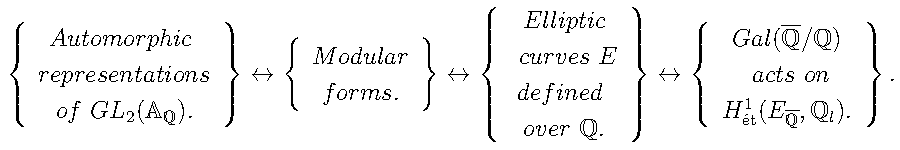
\includegraphics[width=0.7257\paperwidth]{images/L6-p043-correspondence.pdf}\end{figure}
因此，现在该讨论模形式了。取$G=\GL_2$。
\section{模形式}\label{L6S1}\idx{模形式}
模形式\znote{模形式可以理解为「$\mathcal H$ 上变换规律由权 $k$ 决定的全纯函数」。权 $k$ 的几何含义是：$f(z)(\mathrm dz)^{k/2}$ 在 $\Gamma$-作用下不变，因此模形式是模曲线上的截面；等价地，$k$ 对应 $\SO_2(\R)$ 的一个特征。按 nLab 的说法，模形式常被称为「经典自守形式」，第 2 节将把它对应到 $\mathcal A_0(G)$ 中的向量。[来源：nLab "modular form"，\url{https://ncatlab.org/nlab/show/modular+form}（Last revised 2025-03-13；2026-11-14 访问）。]}是定义在上半平面$\mathcal H:=\{z\in\C\mid\Impart z>0\}$上的全纯函数。另一方面，$G(\R)^+=\{g\in G(\R)\mid\det g>0\}$通过如下方式作用于$\mathcal H$：
\[g=\begin{pmatrix}a&b\\c&d\end{pmatrix}\in G(\R)^+,\qquad g(z):=\frac{az+b}{cz+d}.\]
容易验证，$g_2(g_1(z))=(g_2g_1)(z)$，且\[\Impart(g(z))=\frac{\det g}{|cz+d|^2}\Impart z.\]于是，由$g\mapsto g(i)$得到同构\[\SL_2(\R)/\SO_2(\R)\xrightarrow{\sim}\mathcal H.\]因此，$\mathcal H$上的函数$f$可转化为$\SL_2(\R)$上的函数$F$，定义为$F(g)=f(g(i))$。
\sourcepage{44}
函数$F$还在右$\SO_2(\R)$作用下不变。

不过，正如\eref{引理}{L4S2O2}所示，我们要描述的是$\GL_2(\R)^+$上左$\Gamma$-不变的函数，其中$\Gamma$为某个同余子群\znote{同余子群指 $\SL_2(\Z)$ 中由「模 $n$ 同余条件」切出的子群；等价地，它是某个投影 $\SL_2(\Z)\to\SL_2(\Z/n\Z)$ 之下子群的原像。主同余子群 $\Gamma(n)$ 正是这个投影的核；另有两个常用特例：$\Gamma_0(N)$ 要求下三角元 $\equiv0\pmod N$，$\Gamma_1(N)$ 还要求对角元 $\equiv1$。它们都有限指数，因此 $\Gamma\backslash\mathcal H$ 是复曲线。[来源：nLab "congruence subgroup"，\url{https://ncatlab.org/nlab/show/congruence+subgroup}（Last revised 2026-05-25；2026-11-14 访问）。]}。它形如$\Gamma=G(\Q)\cap(G(\R)^+U)$，其中$U\subseteq G(\A^f)$为满足$\det U=\widehat{\Z}^\times$的紧开子群。可假定$U\subseteq G(\widehat{\Z})$，此时$\Gamma\subseteq\SL_2(\Z)$。

下面取$\Gamma$为Hecke同余子群\znote{「Hecke 同余子群」得名于它对 Hecke 算子封闭：对每个 $n\geq1$，双陪集 $\Gamma_0(N)\begin{pmatrix}n&0\\0&1\end{pmatrix}\Gamma_0(N)$ 给出算子 $T_n$，它保持 $M_k(N)$ 并把 Fourier 系数重新组合；各个 $T_n$ 两两交换，其公共本征函数就是 Hecke 本征形式。本讲只用到 $T_p$ 给出的局部因子，第 8 讲将系统讨论 Hecke 代数。[来源：D. Bump, \textit{Automorphic Forms and Representations}, Cambridge Studies in Advanced Mathematics 55, Cambridge University Press, 2004（本讲参考文献）。]}。设$N$为正整数，
\begin{equation}\tag{1.1}\label{L6eq11}
\Gamma_0(N)=\left\{\begin{pmatrix}a&b\\c&d\end{pmatrix}\in\SL_2(\Z)\ \middle|\ c\equiv0\pmod N\right\}.
\end{equation}
$\Gamma$是与下列紧开子群$U^\Gamma$相对应的同余子群：
\begin{equation}\tag{1.2}\label{L6eq12}
U^\Gamma=U^N=\prod_p\left\{\begin{pmatrix}a&b\\c&d\end{pmatrix}\in\GL_2(\Z_p)\ \middle|\ \ord_p(c)\geq\ord_p(N)\right\}.
\end{equation}
注意，$\mathbb P^1(\Q)\cong G(\Q)/B(\Q)$，其中$B(\Q)$是$G(\Q)$中上三角矩阵组成的Borel子群。
% [Tutor Note: 原书 p44 把 $B(\Q)$ 说成 $G(\R)$ 中上三角矩阵组成的子群，译文按 $B(\Q)\subseteq G(\Q)$ 处理。]
同构由
\[\GL_2(\Q)\ni\begin{pmatrix}a&b\\c&d\end{pmatrix}\longmapsto[a:c]\]
诱导。$\Gamma$的一个\textbf{尖点}是$\mathbb P^1(\Q)$中的一个$\Gamma$-轨道。若$N=1$，则$\Gamma=\SL_2(\Z)$，只有一个尖点$\infty$。一般地，尖点个数为$|\Gamma\backslash\SL_2(\Q)/B_{\SL_2}(\Q)|$，这是有限的；添加这些尖点便可将$\Gamma\backslash\mathcal H$紧化：
\[\overline{\Gamma\backslash\mathcal H}=\Gamma\backslash(\mathcal H\cup\Q\cup\{\infty\}).\]
\idx{尖点}
\originalnumber{1}
\begin{definition}{全纯模形式}\label{L6S1O1}
$\Gamma$的一个\textbf{全纯模形式}是$\mathcal H$上的全纯函数$f$，满足以下两个性质：
\begin{itemize}
\item （自守性）对任意$\gamma=\begin{pmatrix}a&b\\c&d\end{pmatrix}\in\Gamma$，有$f(\gamma(z))=(cz+d)^k f(z)$，其中$k$为正整数，称为$f$的\textbf{权}；
\sourcepage{45}
\item （全纯性）$f$在$\Gamma$的每个尖点处都全纯。
\end{itemize}
当$\Gamma=\Gamma_0(N)$时，$N$称为$f$的\textbf{级}。若$f$还在每个尖点处为零，就称它为\textbf{尖点形式}，或称$f$具有尖点性。
\end{definition}
\idx{权（模形式）}\idx{级（模形式）}\idx{尖点形式}
\originalnumber{2}
\begin{note}[L6S1O2]
\begin{enumerate}
\item 若$k$为奇数，则$f$必为零，因为$\begin{pmatrix}-1&0\\0&-1\end{pmatrix}\in\Gamma$。
\item 因$t=\begin{pmatrix}1&1\\0&1\end{pmatrix}\in\Gamma$，有$f(z+1)=f(z)$。因此$f$实际上可看成带状区域$\{x+iy\mid-1/2\leq x\leq1/2,\ y>0\}$上的函数。
\item 作变量代换$z\mapsto q=e^{2\pi iz}$，得到$f$在$q=0$附近的Laurent展开\znote{$q=e^{2\pi iz}$ 是尖点 $i\infty$ 处的局部坐标：它把上半平面映到去心圆盘，$z\to i\infty$ 对应 $q\to0$，而带形区域 $\{0<\Re z<1\}$ 映到 $0<|q|<1$。所谓「$f$ 在尖点全纯」，就是它的 Laurent 展开没有负幂项。于是模形式等价于一列满足自守关系的系数 $a_n$，Hecke 本征值与 $L$ 函数这些算术信息全部装在这一列系数里。[来源：nLab "modular form"，\url{https://ncatlab.org/nlab/show/modular+form}（Last revised 2025-03-13；2026-11-14 访问）。]}
\[f(z)=f(q)=\sum_n a_nq^n.\]
由于$f$在$i\infty$处全纯，$f(q)$在$q=0$处全纯，故上式中$n<0$时$a_n=0$。于是$f$有Fourier级数展开
\[f(z)=f(q)=\sum_{n\geq0}a_n(f)q^n.\]
数列$\{a_n(f)\}$称为$f$在尖点$\infty$处的Fourier系数。
\item $f$为尖点形式，当且仅当它在每个尖点处的Fourier展开都满足$a_0(f)=0$。注意，每个尖点都可以通过$\SL_2(\Z)$的某个元素移到$\infty$。
\end{enumerate}
\end{note}
对$f\in M_k(\Gamma)$，若存在$n$和$C$，使当$y\to\infty$且$x$有界时，有$|f(x+iy)|\leq Cy^n$，就说$f$在尖点$i\infty$处\textbf{适度增长}。由Fourier展开，$f$在$i\infty$处适度增长，当且仅当它在$i\infty$处全纯。把其他尖点移到$\infty$，也可对它们定义同样的性质。
\sourcepage{46}
记$M_k(N)$为$\Gamma_0(N)$的所有全纯模形式组成的空间，$S_k(N)$为其中的尖点形式空间。这些复向量空间都是有限维的！此外，$\bigoplus_kM_k(N)$具有环结构，因为若$f_j\in M_{k_j}(N)$（$j=1,2$），则$f_1f_2\in M_{k_1+k_2}(N)$。
\needspace{4\baselineskip}\originalnumber{3}
\begin{example}\label{L6S1O3}\idx{Eisenstein级数}
对$k>1$，归一化Eisenstein级数\znote{Eisenstein 级数是「显式可算」的模形式：$G_4$ 与 $G_6$ 通过 $g_2=60G_4$、$g_3=140G_6$ 给出椭圆曲线的不变量，$\Delta=g_2^3-27g_3^2$ 与 $j=1728g_2^3/\Delta$ 由此把椭圆曲线的同构类读成模形式。第 7 讲会把这条线索变成「模形式 $\leftrightarrow$ 椭圆曲线」的对应；本节只需知道它是 $\Gamma_0(N)$ 上最具体的一类例子。[来源：nLab "Eisenstein series"，\url{https://ncatlab.org/nlab/show/Eisenstein+series}（Last revised 2014-03-26；2026-11-14 访问）。]}
\[E_{2k}(z)=\frac1{2\zeta(2k)}\sum_{\substack{(c,d)\in\Z^2\\(c,d)\ne(0,0)}}\frac1{(cz+d)^{2k}}\]
是$\SL_2(\Z)$的权$2k$模形式，其Fourier展开为
\[E_{2k}(z)=1-\frac{4k}{B_{2k}}\sum_{n=1}^{\infty}\sigma_{2k-1}(n)q^n.\]
这里$\zeta(s):=\sum_{n=1}^{\infty}n^{-s}$为Riemann的$\zeta$函数，$B_{2k}$为第$2k$个Bernoulli数，$\sigma_r(n):=\sum_{d\mid n}d^r$\znoteplain{判别这类公式对不对，最快的办法是代入最小的 $k$ 验算。$k=2$ 时 $B_4=-1/30$，$-4k/B_{2k}=8/(1/30)=240$，得 $E_4=1+240q+\cdots$；$k=3$ 时 $B_6=1/42$，$-4k/B_{2k}=-12/(1/42)=-504$，得 $E_6=1-504q+\cdots$。这两个展开必须与 $G_4=1+240q+\cdots$、$G_6=1-504q+\cdots$ 的系数一致。若误用第 $k$ 个 Bernoulli 数（$B_2=1/6$），$k=2$ 会算出 $48$，$q$ 展开随之出错——所以下标是 $B_{2k}$ 而非 $B_k$，符号也是负的。（上下文推断，无外部依据）}。
% [Tutor Note: 原书 p46 印作 $1+(-1)^k4k/B_k\cdot\sum\sigma_{2k-1}(n)q^n$ 并称「$B_k$ are the so-called nth Bernoulli number」；此处 Bernoulli 数下标应为 $2k$、符号应为负号，按标准写法 $1-4k/B_{2k}\sum\sigma_{2k-1}(n)q^n$ 处理（代入 $k=2,3$ 得 $E_4=1+240q+\dots$、$E_6=1-504q+\dots$ 可验证）。]
\end{example}
对偶数$k\geq4$，还满足$M_k(1)=\C E_k\oplus S_k(1)$。
\originalnumber{4}
\begin{example}\label{L6S1O4}\idx{Theta函数}
另一个重要例子是Theta函数。设$A$为$k$阶正定对称整数矩阵。假定$A$为偶矩阵，即对所有$x\in\Z^k$，$x^TAx$均为偶数，并且$\det A=1$。定义二次型$Q(x):=\tfrac12x^TAx$。级数
\[\theta_Q(z)=\sum_{x\in\Z^k}q^{Q(x)}=\sum_{n\geq0}a_n(Q)q^n,\]
其中$q=e^{2\pi iz}$，$a_n(Q)=|\{x\in\Z^k\mid Q(x)=n\}|$，是权$k/2$、级$1$的模形式。
\end{example}
\begin{exercise*}\label{L6S1EX}
证明：若$f\in M_k(n)$，则对任意满足$n\mid N$的$N$，都有$f\in M_k(N)$。
\par 提示：因为$\Gamma_0(N)\subseteq\Gamma_0(n)$，自守条件容易验证。对于全纯条件，利用以下事实：$\Gamma_0(N)$的每个尖点都可通过$\Gamma_0(n)$的某个元素移到$\Gamma_0(n)$的一个尖点。
\end{exercise*}
\sourcepage{47}
事实上，若$f\in M_k(n)$，取正整数$m$并令$h(z)=f(mz)$，则对任意满足$mn\mid N$的$N$，都有$h\in M_k(N)$。这里只验证自守条件。对任意$\begin{pmatrix}a&b\\c&d\end{pmatrix}\in\Gamma_0(N)$，有
\begin{align*}
h\!\left(\begin{pmatrix}a&b\\c&d\end{pmatrix}(z)\right)
&=f\!\left(m\begin{pmatrix}a&b\\c&d\end{pmatrix}(z)\right)
=f\!\left(\begin{pmatrix}a&mb\\c/m&d\end{pmatrix}(mz)\right)\\
&=\left(\frac cm mz+d\right)^k f(mz)=(cz+d)^k h(z).
\end{align*}
第二行的等式成立，是因为$\begin{pmatrix}a&mb\\c/m&d\end{pmatrix}\in\Gamma_0(n)$且$f\in M_k(n)$。
% [Tutor Note: 原书 p47 把这里的指数误作 $2k$（$\frac{1}{((c/m)mz+d)^{2k}}$ 与 $\frac{1}{(cz+d)^{2k}}$），译文按 $k$ 处理。]
称由$f(mz)$（$f\in M_k(n)$，$n<N$且$mn\mid N$）张成的$M_k(N)$的子空间为\textbf{旧形式空间}；其尖点部分在$S_k(N)$中的正交补称为\textbf{新形式空间}\znoteplain{注意区分「新形式空间」与「新形式」：前者是 $S_k(N)$ 中与旧形式空间正交的子空间，后者通常指该空间里归一化（$a_1=1$）的 Hecke 本征形式。定理 3.1 会说明新形式空间由这些 $f_0(\pi)$ 张成，所以文献里的「新形式」往往直接指归一化本征形式，而不是空间中的任意元素。（上下文推断，无外部依据）}。这里的正交性关于仅在$S_k(N)$上定义的Petersson内积：\idx{旧形式}\idx{新形式}\idx{Petersson内积}
\[\langle f_1,f_2\rangle_k:=\int_{\Gamma\backslash\mathcal H}f_1(z)\overline{f_2(z)}\,y^{k-2}\,dx\,dy,\qquad z=x+iy.\]
本节最后给出一个估计尖点形式的Fourier系数的命题。后面不会用到这个命题，但由于证明是初等的，仍在这里介绍。
\originalnumber{5}
\begin{proposition}\label{L6S1O5}
若$f\in S_k(N)$，$a_n(f)$为其Fourier系数，则存在$C_f$，使$|a_n(f)|\leq C_fn^{k/2}$，对所有$n\geq1$成立。
\end{proposition}
\begin{proof}
回忆，对$g=\begin{pmatrix}a&b\\c&d\end{pmatrix}$，有$\Impart(g(z))=\frac{\det g}{|cz+d|^2}\Impart z$。令$F(z)=(\Impart z)^{k/2}|f(z)|$，则
\[F(\gamma z)=(\Impart(\gamma z))^{k/2}|f(\gamma z)|=(\Impart z)^{k/2}|f(z)|=F(z).\]
因此$F$为$\Gamma\backslash\mathcal H$上的连续函数。此外，$f$全纯，当$z\to i\infty$时趋于零，从而$F(z)\to0$。故$F$在$\mathcal H$上有界，因而存在$C_f$，使$|f(x+iy)|\leq C_fy^{-k/2}$。固定$y$，有
\[|a_n(f)e^{-2\pi ny}|=\left|\int_0^1e^{-2\pi inx}f(x+iy)\,dx\right|\leq\int_0^1|f(x+iy)|\,dx.\]
于是$|a_n(f)|\leq C_fe^{2\pi ny}y^{-k/2}$。取$y=1/n$并调整常数，即得结论。
% [Tutor Note: 原书 p47 作 $|a_n(f)e^{2\pi ny}|$ 与 $|a_n(f)|\leq C_fe^{-2\pi ny}y^{-k/2}$，指数符号有误，译文按 $e^{-2\pi ny}$、$e^{2\pi ny}$ 处理。]
\end{proof}
\sourcepage{48}
\section{从模形式到自守表示}\label{L6S2}
现在由$f\in M_k(N)$构造$G(\R)^+$上的左$\Gamma$-不变函数$\phi_f$。
\originalnumber{1}
\begin{definition}{余循环}\label{L6S2O1}\idx{余循环}
设群$G$作用于集合$S$。$G\times S$上的一个\textbf{余循环}是函数$J:G\times S\longrightarrow\C$，满足$J(\alpha\beta,s)=J(\alpha,\beta\cdot s)J(\beta,s)$，对所有$\alpha,\beta\in G$和$s\in S$成立。
\end{definition}
令$j:G(\R)^+\times\mathcal H\longrightarrow\C$，对$\gamma=\begin{pmatrix}a&b\\c&d\end{pmatrix}$，定义$j(\gamma,z)=(cz+d)^k(\det\gamma)^{-k/2}$。则$j$在$\Gamma\times\mathcal H$上为余循环。对$f\in M_k(N)$，令$\phi_f(g)=j(g,i)^{-1}f(g(i))$，于是$\phi_f$是$G(\R)^+$上的左$\Gamma$-不变函数。
\originalnumber{2}
\begin{lemma}\label{L6S2O2}
对$f\in M_k(N)$，经阿代尔化延拓后$\phi_f\in\mathcal A(G)$。此外，$\phi_f\in\mathcal A_0(G)$当且仅当$f\in S_k(N)$。
\end{lemma}
\begin{proof}
需要检查\eref{定义}{L4S3O1}中的所有条件。(i)、(ii)、(v)、(vi)显然成立。注意，$\phi_f$看成$G(\A)$上的函数时是左$G(\Q)$-不变的；$K$-有限性来自$i$被$\SO(2)$固定。

对于(iii)，$\phi_f$的适度增长自然来自上一节定义的$f$的适度增长。

对于(iv)，$U(\mathfrak{sl}_2(\C))$的中心由Casimir元素
\[C=H^2+2X_+X_-+2X_-X_+\]
生成，其中$X_\pm=\tfrac12\begin{pmatrix}1&\pm i\\\pm i&-1\end{pmatrix}\in\g$，$H=\begin{pmatrix}0&-i\\i&0\end{pmatrix}\in\g$。需要检查$C$对$\phi_f$的作用。由定义，
\[H\cdot\phi_f(g)=i\begin{pmatrix}0&-1\\1&0\end{pmatrix}\cdot\phi_f(g).\]
\sourcepage{49}
注意，
\begin{align*}
E_H(t)&:=\exp\!\left(t\begin{pmatrix}0&-1\\1&0\end{pmatrix}\right)\\
&=\begin{pmatrix}\displaystyle\sum_{r\geq0}\frac{(-1)^rt^{2r}}{(2r)!}&\displaystyle-\sum_{r\geq0}\frac{(-1)^rt^{2r+1}}{(2r+1)!}\\\displaystyle\sum_{r\geq0}\frac{(-1)^rt^{2r+1}}{(2r+1)!}&\displaystyle\sum_{r\geq0}\frac{(-1)^rt^{2r}}{(2r)!}\end{pmatrix}\\
&=\begin{pmatrix}\cos t&-\sin t\\\sin t&\cos t\end{pmatrix}\in\SO(2).
\end{align*}
于是$E_H(t)(i)=i$，且
\begin{align*}
\left.\frac d{dt}\phi_f(gE_H(t))\right|_{t=0}
&=\left.\frac d{dt}\{j(g,i)^{-1}j(E_H(t),i)^{-1}f(g(i))\}\right|_{t=0}\\
&=-ik\phi_f(g).
\end{align*}
因此$H\cdot\phi_f=k\phi_f$，$H^2\cdot\phi_f=k^2\phi_f$。由\eref{引理}{L6S2O3}，$X_-\cdot\phi_f=0$。又因$[X_+,X_-]=H$，
\[2(X_+X_-+X_-X_+)\cdot\phi_f=2(-H+2X_+X_-)\cdot\phi_f=-2H\cdot\phi_f=-2k\phi_f.\]
于是$C\cdot\phi_f=(k^2-2k)\phi_f$。因此$\phi_f$是$C$的特征向量，当然是$Z(\g)$-有限的。
% [Tutor Note: 原书 p49 作 $H\cdot\phi_f(g)=H\cdot(H\cdot\phi_f(g))=k\phi_f(g)$ 与 $2(-H+2X_+X_-)\cdot\phi_f=-2H\cdot\phi_f=2k\phi_f$，记号重复、符号亦有误，译文按 $H\cdot\phi_f=k\phi_f$、$H^2\cdot\phi_f=k^2\phi_f$、$-2H\cdot\phi_f=-2k\phi_f$ 处理。]

最后检查尖点条件(vii)。这里$N$是形如$n(x)=\begin{pmatrix}1&x\\0&1\end{pmatrix}$的幺幂子群。相应的积分为
\[(\phi_f)_N(g)=\int_{N(\Q)\backslash N(\A)}\phi_f(ng)\,dn=\int_{(N(\Q)\cap\Gamma)\backslash N(\R)}j(ng,i)^{-1}f(ng(i))\,dn.\]
对$n=n(x)$，有$n(g(i))=g(i)+x$、$j(ng,i)=j(g,i)$，且$N(\Q)\cap\Gamma=N(\Z)$。因此
\[(\phi_f)_N(g)=\int_{\Z\backslash\R}j(g,i)^{-1}f(g(i)+x)\,dx=j(g,i)^{-1}\int_0^1f(g(i)+x)\,dx.\]
% [Tutor Note: 原书 p49 的这两个积分式写作 $j(g,i)f(g(i)+x)$，漏了指数 $-1$，译文按 $j(g,i)^{-1}$ 处理。]
利用Fourier展开$f(z)=\sum_{n\geq0}a_ne^{2\pi inz}$，得到$(\phi_f)_N(g)=j(g,i)^{-1}a_0$。因此，$\phi_f$具有尖点性，当且仅当$f$具有尖点性。
\end{proof}
\originalnumber{3}
\begin{lemma}\label{L6S2O3}
满足\eref{定义}{L6S1O1}中自守条件的光滑函数$f:\mathcal H\longrightarrow\C$全纯，当且仅当$X_-\phi_f=0$。
\end{lemma}
\sourcepage{50}
\begin{proof}
由定义，
\[X_-\cdot\phi_f(g)=\frac12\begin{pmatrix}1&0\\0&-1\end{pmatrix}\cdot\phi_f(g)-\frac i2\begin{pmatrix}0&1\\1&0\end{pmatrix}\cdot\phi_f(g).\]
还有
\begin{align*}
E_1(t)&:=\exp\!\left(t\begin{pmatrix}0&1\\1&0\end{pmatrix}\right)\\
&=\begin{pmatrix}\displaystyle\sum_{r\geq0}\frac{t^{2r}}{(2r)!}&\displaystyle\sum_{r\geq0}\frac{t^{2r+1}}{(2r+1)!}\\\displaystyle\sum_{r\geq0}\frac{t^{2r+1}}{(2r+1)!}&\displaystyle\sum_{r\geq0}\frac{t^{2r}}{(2r)!}\end{pmatrix}
=\begin{pmatrix}\cosh t&\sinh t\\\sinh t&\cosh t\end{pmatrix},\\
E_2(t)&:=\exp\!\left(t\begin{pmatrix}1&0\\0&-1\end{pmatrix}\right)=\begin{pmatrix}e^t&0\\0&e^{-t}\end{pmatrix}.
\end{align*}
直接计算得到
\[X_-\cdot\phi_f(g)=\frac{-2i\det g}{(ci-d)^2}j(g,i)^{-1}\frac{\partial f}{\partial\overline z}(g(i)).\]
于是引理成立。
\end{proof}
现在有映射$M_k(N)\longrightarrow\mathcal A(G)$，$f\mapsto\phi_f$，把$S_k(N)$识别为$\mathcal A_0(G)$的一个子空间。$S_k(N)$尚不足以描述$\mathcal A_0(G)$中出现的所有不可约表示，需要构造更多自守形式。
\originalnumber{4}
\begin{definition}{Dirichlet特征标}\label{L6S2O4}\idx{Dirichlet特征标}
模$N$的\textbf{Dirichlet特征标}$\chi_N$是函数$\chi_N:\Z\longrightarrow\C$，满足：
\begin{itemize}
\item 若$(n,N)>1$，则$\chi_N(n)=0$；且$\chi_N(1)=1$。特别地，$N>1$时$\chi_N(0)=0$。
\item （周期为$N$）若$n\equiv n'\pmod N$，则$\chi_N(n)=\chi_N(n')$。
\item （完全乘法性）对所有$n,m\in\Z$，$\chi_N(nm)=\chi_N(n)\chi_N(m)$。
\end{itemize}
% [Tutor Note: 原书 p50 的定义只列了 $\chi_N(0)=0$，译文按通常定义（$(n,N)>1$ 时 $\chi_N(n)=0$，且 $\chi_N(1)=1$）处理。]
\end{definition}
设$f$如\eref{定义}{L6S1O1}，但将其中的自守条件替换为下述条件。
\begin{property}\textbf{（带特征标的自守性）}
对$\gamma=\begin{pmatrix}a&b\\c&d\end{pmatrix}\in\Gamma_0(N)$，有$f(\gamma(z))=\chi_N(d)(cz+d)^k f(z)$。
\end{property}
\sourcepage{51}
此时称$f$为\textbf{带特征标$\chi_N$的模形式}。记$S_k(N,\chi_N)$为所有带特征标$\chi_N$的尖点模形式组成的空间。若$\chi_N$在$(\Z/N\Z)^\times$上恒为$1$，则$S_k(N,\chi_N)=S_k(N)$。若$S_k(N,\chi_N)$含有非零元素，则$\chi_N(-1)=(-1)^k$。同样有映射$f\mapsto\phi_f$，但$\phi_f$起初只是$G(\R)^+$上的函数。

取\eqref{L6eq12}中的$U^N$。通过中国剩余定理把$\chi_N$分解为各$p\mid N$处的特征标$\chi_p$，则它在$U^N$上诱导特征标$\chi$，定义为
\[\chi\!\left(\left(\begin{pmatrix}a_p&b_p\\c_p&d_p\end{pmatrix}\right)_p\right):=\prod_{p\mid N}\chi_p(a_p).\]
把$\phi_f$延拓为$G(\A)$上的函数，也就得到$\mathcal A_0(G)$中的元素，定义为
\[\phi_f(\alpha)=\phi_f(\beta\alpha_\infty k_\alpha):=\phi_f(\alpha_\infty)\chi(k_\alpha),\]
其中$\beta\in G(\Q)$、$k_\alpha\in U^N$，且$\alpha=\beta\alpha_\infty k_\alpha$。由此，$S_k(N,\chi_N)$也可识别为$\mathcal A_0(G)$的子空间。
\section{从局部到整体}\label{L6S3}
我们已经知道，每个不可约尖点自守表示$\pi$都形如$\pi=\pi_\infty\otimes(\bigotimes_p'\pi_p)$，各$\pi_p$和$\pi_\infty$不可约可容许，且几乎所有$\pi_p$非分歧。由强重数一性质，可以取$\pi_\infty\cong\operatorname{DS}_k$。设$\omega_p$为$\pi_p$的中心特征标，$c(\pi_p)$为其导子指数。前面已见，若$\pi_p$非分歧，则$c(\pi_p)=0$。
% [Tutor Note: 原书 p51 作 $c(\pi_p)=1$ 当 $\pi_p$ 非分歧，与 $N(\pi)=\prod_p p^{c(\pi_p)}$ 的定义不自洽，译文按 $c(\pi_p)=0$ 处理。]
定义\idx{导子（自守表示）}
\[N(\pi)=\prod_p p^{c(\pi_p)}.\]
由\eref{定理}{L5S3O6}，空间
\[\mathcal A_0(\pi)_{\mathrm{hol}}^{\mathrm{new}}:=\left\{\phi\in\mathcal A_0(\pi)\ \middle|\ \begin{array}{l}\text{(i) }X_-\phi=0,\\\text{(ii) }\phi(gu)=\omega(u)\phi(g),\quad u\in U^{N(\pi)}\end{array}\right\}\]
的维数至多为$1$。容易看出$\mathcal A_0(\pi)_{\mathrm{hol}}^{\mathrm{new}}\subseteq S_k(N(\pi),\chi_{N(\pi)})$，其中$\chi_{N(\pi)}$由$\prod_{p\mid N(\pi)}\omega_p$在单位群上的限制诱导。设$f_0\in S_k(N(\pi),\chi_{N(\pi)})$为$\mathcal A_0(\pi)_{\mathrm{hol}}^{\mathrm{new}}$这个一维空间的一个基向量。由重数一性质，$f_0$在数乘意义下由$\pi$唯一确定。回忆，\sref{L6S1}已经定义了新形式与旧形式。记$S_k(N,\chi_N)^{\mathrm{new}}$为这些新形式张成的空间。
% [Tutor Note: 原书 p51 作 "newforms and oddforms"，应为 oldforms，译文按「旧形式」处理。]
\sourcepage{52}
\needspace{4\baselineskip}\originalnumber{1}
\begin{theorem}\label{L6S3O1}
\begin{enumerate}
\item 与自守表示$\pi$相伴的$f_0(\pi)$是一个新形式。
\item 设$\omega$为与$\chi_N$相对应的Hecke特征标，其有限分量为$\prod_p\omega_p$。则
\[S_k(N,\chi_N)^{\mathrm{new}}\cong\bigoplus_{\substack{\pi\\\omega_\pi=\omega\\\pi_\infty\cong\operatorname{DS}_k\\N(\pi)=N}}\mathcal A_0(\pi)_{\mathrm{hol}}^{\mathrm{new}}.\]
因此，每个新形式在数乘意义下都是某个$f_0(\pi)$。
\item 此外，
\[S_k(N,\chi_N)\cong\bigoplus_{\substack{\pi\\\omega_\pi=\omega\\\pi_\infty\cong\operatorname{DS}_k\\N(\pi)\mid N}}\mathcal A_0(\pi)_{\mathrm{hol}}^N,\]
其中$\mathcal A_0(\pi)_{\mathrm{hol}}^N$是在$\mathcal A_0(\pi)_{\mathrm{hol}}^{\mathrm{new}}$的定义中，把条件(ii)中的$N(\pi)$替换为$N$而得到的空间。
\end{enumerate}
\end{theorem}
\originalnumber{2}
\begin{note}[L6S3O2]
一般而言，$\pi$是无限维的，但我们用它在几乎所有$p$处的$U_p^N$-不变子空间（有限维）来分类这些无限维表示。考虑到强重数一性质与局部表示的Hecke理论，这一现象十分自然。
\end{note}
\needspace{5\baselineskip}\section{第6讲参考文献}\label{L6S4}
\needspace{4\baselineskip}关于模形式：
\begin{references}\refitem{L6refB2}{B2} D. Bump, \textit{Automorphic Forms and Representations}, Cambridge Studies in Advanced Mathematics 55, Cambridge University Press, 2004.
% [Tutor Note: 原书 p52 的文献条目把书名拼作 "Automophic"，译文按正确拼写处理。]
\end{references}
\needspace{4\baselineskip}关于由模形式得到的自守表示：
\begin{references}\refitem{L6refBG}{BG} J. Bernstein and S. Gelbart, eds, \textit{An introduction to the Langlands Program}, Birkh\"auser, 2004, Chapter 7 written by Stephen S. Kudla.\end{references}

\addtocontents{toc}{\protect\newpage}
\chapter{Galois表示之一：椭圆曲线的\texorpdfstring{$\ell$}{ℓ}进表示}\label{L7}
\lecturedate{2020/03/09}
\sourcepage{53}
本讲讨论$\Gal(\overline{\Q}/\Q)$的Galois表示。域$F$上的椭圆曲线$E$的Tate模，给出了$\Gal(\overline F/F)$的一个$\ell$进表示，其中$\ell$为与$\operatorname{char}(F)$互素的素数。借助Hasse--Weil $L$函数，可以把这些$\ell$进表示与模形式联系起来。不过，要充分揭示模形式在这里的作用，需要把某个Hecke代数上的秩2自由模实现为椭圆曲线的模空间——模曲线——上的某些上同调群，由此得到Galois表示。
\section{椭圆曲线}\label{L7S1}
先简要介绍椭圆曲线。

\textbf{域上的椭圆曲线。}在特征不为2、3的域$F$上，可以先用仿射平面中的下列非奇异曲线来介绍椭圆曲线\znote{「椭圆曲线」指亏格为 $1$ 的射影代数曲线，并指定一个有理点 $O$ 作为基点；下面的 Weierstrass 形式是它在特征不为 $2$、$3$ 时的仿射写法。特征 $2$、$3$ 时不能化成书中这种短的 Weierstrass 形式，需要一般的 $y^2+a_1xy+a_3y=x^3+a_2x^2+a_4x+a_6$；无论采用哪种写法，「椭圆曲线」都要求判别式 $\Delta\ne0$，即曲线非奇异。[来源：J. H. Silverman, \textit{The arithmetic of elliptic curves}, 2nd ed., GTM 106, 第 III 章（本讲参考文献 [S]）；并见 nLab "elliptic curve"，\url{https://ncatlab.org/nlab/show/elliptic+curve}（Last revised 2025-05-11；2026-11-14 访问）。]}$E$：
\begin{align*}
y^2&=x^3+ax^2+bx+c\\
&=\left(x+\frac a3\right)^3+\left(b-\frac{a^2}3\right)\left(x+\frac a3\right)+\left(c-\frac{ab}3+\frac{2a^3}{27}\right),\qquad a,b,c\in F.
\end{align*}
作保持$F$有理点的变量代换，也可以采用Weierstrass形式
\[y^2=x^3+ax+b,\qquad a,b\in F.\]
令$f(x,y)=x^3+ax^2+bx+c-y^2$。曲线$E$非奇异，当且仅当下列方程组在$\overline F$中无解：
\[f(x,y)=0,\qquad \frac{\partial f}{\partial x}(x,y)=0,\qquad \frac{\partial f}{\partial y}(x,y)=0.\]
仿射曲线$E$不是完备的；添加无穷远点$\infty$可得到其射影完备化。
\sourcepage{54}
完备化$\overline E$上的群结构定义如下：
\begin{itemize}
\item 对于$P\ne Q\in E$，过$P,Q$的直线$\ell(P,Q)$与曲线的第三个交点记为$R'$。将$R'$关于$x$轴对称，得到点$R$，定义$P+Q=R$。
\item 当$P=Q$时，采用曲线在$P$处的切线，并按上述第三交点及对称规则定义$P+P$。
% [Tutor Note: 原书 p54 作 "If P = Q, then we define P + P = ∞"；但 $P+P=\infty$ 只在 $y(P)=0$ 时成立，译文按 $P$ 处切线的第三交点处理。]
\item 对每个$P\in\overline E$，都有$\infty+P=P$。
\end{itemize}
上述运算确实给出良定义的群法则，这一点并不显然，因为结合律并不能从定义中直接看出。
\originalnumber{1}
\begin{definition}{$j$不变量}\label{L7S1O1}\idx{j不变量}
以Weierstrass形式$y^2=x^3+ax+b$给出的椭圆曲线$E$的\textbf{$j$不变量}\znote{$j$ 的模性可以这样看：$\C/\Lambda$ 的 $j$ 只取决于格 $\Lambda$ 的相似类，所以它是上半平面在上半平面模群作用下的函数。两个特殊值值得记住：$j=0$ 时 $g_2=0$，对应格 $\Z+\Z e^{2\pi i/3}$，自同构群为 $\Z/6$；$j=1728$ 时 $g_3=0$，对应 Gauss 格 $\Z+\Z i$，自同构群为 $\Z/4$；其余复椭圆曲线的自同构群都只有 $\{\pm1\}$。$j\to\infty$（即 $\Delta\to0$）对应结点曲线，是紧化模空间时补上的尖点。[来源：nLab "j-invariant"，\url{https://ncatlab.org/nlab/show/j-invariant}（Last revised 2015-12-09；2026-11-14 访问）。]}为
\[j(E)=1728\frac{4a^3}{4a^3+27b^2}.\]
\end{definition}
\originalnumber{2}
\begin{theorem}\label{L7S1O2}
设$E,E'$是$F$上的椭圆曲线，则$E$与$E'$在$\overline F$上同构，当且仅当$j(E)=j(E')$。
\end{theorem}
\originalnumber{3}
\begin{note}[L7S1O3]
$j(E)=j(E')$未必意味着$E$与$E'$在$F$上同构。例如，
\[E/\Q:\ y^2=x^3+x;\qquad E'/\Q:\ y'^2=x'^3+49x'.\]
这里$j(E)=j(E')=1728$，然而$E(\Q)$是有限的，$E'(\Q)$则是无限的。它们实际上在$\Q(\sqrt7)$上同构，换元为
\[x=\frac{x'}7,\qquad y=\frac{y'}{7\sqrt7}.\]
% [Tutor Note: 原书 p54 的换元印作 $x=x'/\sqrt7$、$y=y'/(7\sqrt7)$；代入 $y'^2=x'^3+49x'$ 只能得到 $y^2=\frac{\sqrt7}{49}(x^3+7x)$，故 $x$ 应为 $x'/7$，译文按此处理。]
\end{note}
\textbf{复椭圆曲线。}定义在$\C$上的椭圆曲线可以看成一维复环面。

设$\Lambda\subset\C$为格，$\Lambda\cong\Z^2$。商$\C/\Lambda$自然具有紧复流形和加法群的结构。
\originalnumber{4}
\begin{theorem}\label{L7S1O4}
给定格$\Z^2\cong\Lambda\subset\C$，存在与之对应的椭圆曲线$E_\Lambda$，使$\C/\Lambda\cong E_\Lambda(\C)$为复Lie群同构。反过来，给定$F\subset\C$上的椭圆曲线$E$，存在格$\Lambda_E$，使$E(\C)\cong\C/\Lambda_E$为群同构。
\end{theorem}
\sourcepage{55}
给定格$\Z^2\cong\Lambda\subset\C$，与$\Lambda$对应的椭圆函数，亦即Weierstrass $\wp$函数，是
\begin{equation}\tag{1.1}\label{L7eq11}
\wp_\Lambda(z)=\frac1{z^2}+\sum_{\omega\in\Lambda\setminus\{0\}}\left(\frac1{(z-\omega)^2}-\frac1{\omega^2}\right).
\end{equation}
用下列方程定义曲线$E_\Lambda$：
\[y^2=4x^3-g_2(\Lambda)x-g_3(\Lambda),\]
其中
\[g_2(\Lambda)=60\sum_{\omega\in\Lambda\setminus\{0\}}\omega^{-4},\qquad g_3(\Lambda)=140\sum_{\omega\in\Lambda\setminus\{0\}}\omega^{-6}.\]
同构$\C/\Lambda\cong E_\Lambda(\C)$由下列映射给出：
\[z\longmapsto(\wp_\Lambda(z),\wp'_\Lambda(z))\quad(z\notin\Lambda),\qquad z\longmapsto\infty\quad(z\in\Lambda).\]
从椭圆曲线$E$可以得到格$\Lambda=\omega_1\Z\oplus\omega_2\Z$，其中
\[\omega_j=\int_{\alpha_j}\frac{dx}{y},\quad j=1,2,\]
而$\alpha_1,\alpha_2$生成$H_1(E(\C),\Z)$。

若存在$\tau\in\C^\times$使$\Lambda=\tau\Lambda'$，就称$\Lambda$与$\Lambda'$\textbf{位似}。
\originalnumber{5}
\begin{theorem}\label{L7S1O5}
$E_\Lambda(\C)$与$E_{\Lambda'}(\C)$作为复椭圆曲线同构，当且仅当$\Lambda$与$\Lambda'$位似。
\end{theorem}
\originalnumber{6}
\begin{note}[L7S1O6]
任意域上的椭圆曲线，也可以定义为带有一个指定有理点、光滑、射影且几何不可约的亏格 $1$ 曲线，或等价地定义为一维阿贝尔簇。
\end{note}
\section{Tate模与Hasse--Weil \texorpdfstring{$L$}{L}函数}\label{L7S2}\idx{Tate模}\idx{Hasse--Weil L函数}
可以为基概形$S$上的阿贝尔簇$A_S$定义Tate模。它在构造Galois表示时起着关键作用。先讨论域$K$上阿贝尔簇的Tate模\znote{Tate 模可以看成「$\ell$ 进奇异同调」：它把挠点 $A[\ell^n]$ 按 $\ell$ 的幂排成逆向系再取极限，于是群 $A(K^{\mathrm{sep}})$ 的挠部分被线性化成 $\Z_\ell$ 模，Galois 作用也随之变成连续的矩阵作用。Tate 猜想（Faltings 1983 对 Abel 簇证明）断言：两个 Abel 簇之间的同源，恰由它们 Tate 模上 Galois 表示之间的同构给出，可见这个构造不会丢掉几何信息。[来源：J. H. Silverman, \textit{The arithmetic of elliptic curves}, 2nd ed., GTM 106, 第 III 章与第 VII 章（本讲参考文献 [S]）。]}；其中一维阿贝尔簇就是椭圆曲线。

两个阿贝尔簇之间的\textbf{同源}\znote{同源允许丢掉有限核，因此它比同构粗一层。复情形最直观：两个复环面之间的同源，就是满足 $\alpha\Lambda_1\subset\Lambda_2$ 的复数 $\alpha$，于是同源类只由格张量 $\Q$ 之后的结果决定。反过来也有深刻结论：Tate 模上 $\ell$ 进表示的同构必来自同源，这正是 Faltings 证明 Tate 猜想的推论。[来源：J. H. Silverman, \textit{The arithmetic of elliptic curves}, Springer, 2009（本讲参考文献）。]}$A\to A'$，是核有限的满同态。因此，同源只能发生在维数相同的阿贝尔簇之间。同源$\varphi:A\to A'$的次数记为$\deg(\varphi)$，是它作为正则映射的次数，
\sourcepage{56}
即$[k(a):\varphi^*k(a')]$，其中$k(a)$、$k(a')$分别为$A$、$A'$的泛点$a$、$a'$处的剩余域。若$\varphi$可分，则由于群结构的齐性，它是平展的。若$K$进一步为代数闭域，则$\varphi$的每个纤维恰有$\deg(\varphi)$个点。对每个正整数$n$，都有同源
\[n_A:A\longrightarrow A,\qquad x\longmapsto nx.\]
\idx{同源}
\originalnumber{1}
\begin{theorem}\label{L7S2O1}
设$A/K$为$g$维阿贝尔簇，则$\deg(n_A)=n^{2g}$。当$\operatorname{char}(K)=0$时，$n_A$总是平展的；当$\operatorname{char}(K)=p>0$时，它平展当且仅当$p\nmid n$。
\end{theorem}
取$A$上的甚丰沛线丛$\mathcal L$，利用立方定理考察$[n_A]^*\mathcal L$的次数，可以证明\eref{定理}{L7S2O1}。

记$A[n]$为$n_A$的核。由\eref{定理}{L7S2O1}，若$K$可分闭，且$n$与$\operatorname{char}(K)$互素，则$A[n](K)\cong(\Z/n\Z)^{2g}$。

设$\ell\ne\operatorname{char}(K)$为素数，$K^{\mathrm{sep}}$为$K$的可分闭包。于是$A[\ell](K^{\mathrm{sep}})\cong(\Z/\ell\Z)^{2g}$。$A$的Tate模是
\[T_\ell A:=\varprojlim_n A[\ell^n](K^{\mathrm{sep}})\cong\Z_\ell^{2g},\]
$\End(A)$和$\Gal(K^{\mathrm{sep}}/K)$都连续作用于$T_\ell A$。表示
\[\sigma_\ell:\Gal(K^{\mathrm{sep}}/K)\longrightarrow\GL(T_\ell A\otimes_{\Z_\ell}\Q_\ell)\cong\GL_{2g}(\Q_\ell)\]
称为$A$的\textbf{$\ell$进表示}\znote{严格说，$\ell$ 进表示指取 $\Q_\ell$ 系数的连续同态 $G_K\to\GL_n(\Q_\ell)$，故书中真正用作表示的其实是 $V_\ell A:=T_\ell A\otimes_{\Z_\ell}\Q_\ell$；$T_\ell A$ 本身只是 $\Z_\ell$ 模，取 $\Q_\ell$ 系数是为了让迹、行列式与同源都有好的函子性。同理，「$\ell$ 进」与「$\ell$ 可除」是两套语言：$A[\ell^\infty]$ 与 $V_\ell A$ 互为对偶。[来源：J. H. Silverman, \textit{The arithmetic of elliptic curves}, Springer, 2009（本讲参考文献）；并见 nLab "Galois representation"，\url{https://ncatlab.org/nlab/show/Galois+representation}（Last revised 2023-04-21；2026-11-14 访问）。]}。
\originalnumber{2}
\begin{note}[L7S2O2]
若$\varphi:A\to A'$为同源，且$\deg(\varphi)$同时与$\ell$及$\operatorname{char}(K)$互素，则$\varphi$诱导同构$A[\ell^n]\xrightarrow{\sim}A'[\ell^n]$，从而$T_\ell A\cong T_\ell A'$。
\end{note}
\originalnumber{3}
\begin{note}[L7S2O3]
若$A(\C)\cong\C^g/\Lambda_{2g}$为复环面，其中$\Lambda_{2g}\cong\Z^{2g}$，则$A[n]\cong\frac1n\Lambda_{2g}/\Lambda_{2g}$。另一方面，$\Lambda_{2g}\cong H_1(A(\C),\Z)$。因此，$A[\ell^n]\cong H_1(A(\C),\Z/\ell^n\Z)$，且$T_\ell A\cong H_1(A(\C),\Z)\otimes\Z_\ell$。
\end{note}
对任意$\alpha\in\End(A)$，存在一个次数为$2g$的多项式$f_\alpha\in\Z[t]$，称为$\alpha$的\textbf{特征多项式}。它的定义性质是：对所有$n\in\Z$，有$f_\alpha(n)=\deg(n_A-\alpha)$。若
\sourcepage{57}
$\beta:A\to A$不是满射，约定$\deg(\beta)=0$。任意$\alpha\in\End(A)$也作用于$T_\ell A\cong\Z_\ell^{2g}$，因此$\alpha$在$T_\ell A$上诱导矩阵$T_\ell(\alpha)\in M_{2g}(\Z_\ell)$。有如下定理。
\originalnumber{4}
\begin{theorem}\label{L7S2O4}
对任意$\alpha\in\End(A)$，有$\det T_\ell(\alpha)=\deg(\alpha)$。特别地，
\[f_\alpha(t)=\det(tI_{2g}-T_\ell(\alpha)).\]
\end{theorem}
\originalnumber{5}
\begin{note}[L7S2O5]
先验地，$\det(tI_{2g}-T_\ell(\alpha))\in\Z_\ell[t]$。\eref{定理}{L7S2O4}说明，它实际上属于$\Z[t]$，并且只要$\ell$与$\operatorname{char}(K)$互素，就不依赖于$\ell$。
\end{note}
设$p=\operatorname{char}(K)>0$。则$|A[p](\overline K)|=p^r$，其中$0\leq r\leq g$，对一般的$A$有$r=g$。特别地，对$K$上的椭圆曲线$E$，Tate模$T_pE$或者为$\{0\}$，此时称$E$为\textbf{超奇异}\znote{超奇异与普通的区别只在特征 $p$ 上出现，且只依赖 $j$ 不变量。等价刻画是：形式群 $\widehat E$ 的高度为 $2$（超奇异）或 $1$（普通）；也等价于 $E[p](\overline K)=0$（超奇异）或 $E[p](\overline K)\cong\Z/p$（普通）；还等价于 Frobenius 的迹 $a_p\equiv0\pmod p$。对固定的 $p$，超奇异的 $j$ 只有有限多个（$p\ge5$ 时都属于 $\F_{p^2}$）。这个名字容易误导：超奇异曲线本身并不奇异，光滑性一如既往。 [来源：nLab "elliptic curve"，\url{https://ncatlab.org/nlab/show/elliptic+curve}（Last revised 2025-05-11；2026-11-14 访问）。]}椭圆曲线；或者同构于$\Z_p$，此时称$E$为\textbf{普通}椭圆曲线。在代数闭包上，超奇异椭圆曲线的同构类只有有限多个。
\idx{超奇异椭圆曲线}\idx{普通椭圆曲线}
$\Q$上椭圆曲线$E$的Tate模$T_\ell E$给出了$\Gal(\overline{\Q}/\Q)$的一个Galois表示。不过，到目前为止，它似乎还与模形式无关。下面将看到，Hasse--Weil $L$函数以及如今已经成为定理的Shimura--Taniyama--Weil猜想，把二者联系起来。

设$E$为$\Q$上的椭圆曲线。若存在局部环$\Z_{(p)}$上的椭圆曲线$\mathcal E$，其泛纤维$\mathcal E\times_{\Z_{(p)}}\Q$为$E$，就称$E$在素数$p$处具有\textbf{良约化}\znote{「好」与「坏」是相对某个整模型说的：取 $E$ 在 $\Z_{(p)}$ 上的最小 Weierstrass 模型，则好约化当且仅当 $p\nmid\Delta_{\min}$，此时约化曲线仍非奇异。坏约化处导子的指数有明确含义：约化为结点时指数为 $1$，退化为尖点时指数 $\ge2$——这是「坏约化素数只有有限多个」的定量版本。[来源：J. H. Silverman, \textit{The arithmetic of elliptic curves}, Springer, 2009（本讲参考文献）。]}。一般环$R$上的椭圆曲线，是$\Spec R$上一维阿贝尔簇的光滑族$\mathcal E$，并带有零截面$o:\Spec R\hookrightarrow\mathcal E$。特殊纤维$\mathcal E\times_{\Z_{(p)}}\F_p$称为$E$模$p$的约化，记作$E_p$。若$E$在$p$处不具有良约化，就说它具有\textbf{坏约化}。在坏约化素数处，也可以取一个模型，使特殊纤维只有较为“温和”的奇点。$E$只有有限多个坏约化素数。可以给$E/\Q$赋予导子$N_E$，使$p\nmid N_E$当且仅当$E$在$p$处具有良约化。
\idx{良约化}\idx{坏约化}
回忆，对每个素数$p$，都有分解子群$G_{\overline p}\subset\Gal(\overline{\Q}/\Q)$，其中$\overline p$表示$\Q$的所有有限扩张中位于$p$上方的一组相容素理想。惯性群$I_p$是映射
\sourcepage{58}
$G_{\overline p}\cong\Gal(\overline{\Q}_p/\Q_p)\to\Gal(\overline{\F}_p/\F_p)$的核。若$I_p\subset\ker\sigma$，称Galois表示$\sigma$在$p$处\textbf{非分歧}；否则称它在$p$处\textbf{分歧}。
\originalnumber{6}
\begin{theorem}{Ogg--Néron--Shafarevich判别法}\label{L7S2O6}
对$p\ne\ell$，表示$\sigma_\ell:\Gal(\overline{\Q}/\Q)\to\GL(T_\ell E\otimes\Q_\ell)$在$p$处分歧，当且仅当$E$在$p$处不具有良约化。
\end{theorem}
\originalnumber{7}
\begin{note}[L7S2O7]
由\eref{定理}{L7S2O6}可见，只要$\ell\ne p$，$\sigma_\ell$在$p$处是否分歧就不依赖于$\ell$的选择。
\end{note}
\originalnumber{8}
\begin{definition}{Hasse--Weil $L$函数}\label{L7S2O8}
$E/\Q$的Hasse--Weil $L$函数是Euler乘积
\[L(E,s)=\prod_p L_p(E,s),\qquad L_p(E,s)=\det\left(1-p^{-s}\sigma_\ell(\mathrm{Fr}_p)\bigm|(T_\ell E\otimes\Q_\ell)^{I_p}\right)^{-1},\]
其中任取$\ell\ne p$。
\end{definition}
若$E$在$p$处具有良约化，则模$p$约化诱导同构$T_\ell E\cong T_\ell E_p$。此外，算术Frobenius的共轭类$\mathrm{Fr}_p\in\Gal(\overline{\Q}/\Q)$在$T_\ell E_p$上的作用，与曲线的$p$次幂Frobenius态射$F_p:E_p\to E_p$的作用一致，即$T_\ell(F_p)=\sigma_\ell(\mathrm{Fr}_p)$。有
% [Tutor Note: 原书 p58 称 $p$ 次幂态射 $F_p$ 为 "geometric Frobenius"；若取几何 Frobenius（算术 Frobenius 之逆），$T_\ell(F_p)^{-1}$ 的迹为 $a_p/p$，与 $L$ 因子不符，故这里的 $\mathrm{Fr}_p$ 应理解为算术 Frobenius，译文按此处理。]
\[L_p(E,s)=\frac{p^{2s}}{f(p^s)},\qquad f(t)=\det(tI-T_\ell(F_p))=t^2-\Tr(T_\ell(F_p))t+\det(T_\ell(F_p)).\]
% [Tutor Note: 原书 p58 作 $t^2-\operatorname{tr}(T_\ell(F_p)t+\det(T_\ell(F_p)))$，括号位置有误；译文按 $t^2-\operatorname{tr}(T_\ell(F_p))t+\det(T_\ell(F_p))$ 处理。]
记$T_\ell(F_p)$在$\overline{\Q}_\ell$中的两个特征值为$\lambda_p,\lambda'_p$，则$f(t)=t^2-(\lambda_p+\lambda'_p)t+\lambda_p\lambda'_p$，并且
% [Tutor Note: 原书 p58 作 "the two eigenvalue in $\mathbb{Z}_p$"；特征值应在 $\overline{\mathbb{Q}}_\ell$ 中（且应为复数 eigenvalues），译文按此处理。]
\[L_p(E,s)=\bigl(1-(\lambda_p+\lambda'_p)p^{-s}+p^{1-2s}\bigr)^{-1}.\]
由\eref{定理}{L7S2O4}，有$\lambda_p\lambda'_p=\deg(F_p)=p$；由有限域上的Galois理论，还得到
\begin{equation}\tag{2.1}\label{L7eq21}
|E_p(\F_{p^n})|=\deg(1-F_p^n)=1-(\lambda_p^n+\lambda_p'^n)+p^n.
\end{equation}
考察约化曲线的$\zeta$函数
\[Z(E_p,t):=\exp\left(-\sum_{n=1}^\infty\frac{|E_p(\F_{p^n})|}{n}t^n\right).\]
由\eqref{L7eq21}，有
\[Z(E_p,t)=\frac{(1-t)(1-pt)}{1-(\lambda_p+\lambda'_p)t+pt^2},\qquad Z(E_p,p^{-s})=(1-p^{-s})(1-p^{1-s})L_p(E,s).\]
% [Tutor Note: 原书 p58 把 $Z(E_p,p^{-s})$ 印作 $(1-p^{-s})(1-p^{1-s})/L_p(E,s)$，与上一式 $Z(E_p,t)=(1-t)(1-pt)/(1-(\lambda_p+\lambda'_p)t+pt^2)$ 不自洽；按该分式应为相乘，译文按此处理。又：原书把 $\zeta$ 函数定义为 $\exp(-\sum|E_p(\F_{p^n})|t^n/n)$，即通常 Hasse--Weil $\zeta$ 的倒数（用 $t$ 而非 $q^{-s}$ 的形式），与 L8、L9 及通用文献互为倒数，引用时须换算。]
\sourcepage{59}
若$E$在$p$处具有坏约化，$L_p(E,s)$也可以显式写出，共有下列三种情形：
\[L_p(E,s)=\begin{cases}(1-p^{-s})^{-1},&\text{在$p$处具有分裂乘法约化；}\\(1+p^{-s})^{-1},&\text{在$p$处具有非分裂乘法约化；}\\1,&\text{在$p$处具有加法约化。}\end{cases}\]
注意，$L_p(E,s)$不依赖于$\ell$。因此，若$E$与$E'$同源，则由\eref{笔记}{L7S2O2}，有$L(E,s)=L(E',s)$。$L$函数$L(E,s)$有展开
\[L(E,s)=\sum_{n=1}^\infty a_n n^{-s}.\]
定义
\[f_E(q):=\sum_{n=1}^\infty a_nq^n.\]
注意，$a_1=1$，且对几乎所有素数$p$，有$a_p=p+1-|E_p(\F_p)|$。
\originalnumber{9}
\begin{theorem}\label{L7S2O9}
$f_E(q)$是一个权 $2$、级 $N_E$ 的模新形式的 $q$ 展开。
\end{theorem}
\idx{模性定理}
Shimura--Taniyama--Weil猜想还可以表述为比\eref{定理}{L7S2O9}更强的几何命题。我们将看到，在某个参数空间上的椭圆曲线族的Tate模中，这些新形式给出了显式的Galois表示。主要定理如下。
\originalnumber{10}
\begin{theorem}{Eichler--Shimura、Deligne}\label{L7S2O10}
设$N,k$为正整数，$\chi_N:(\Z/N\Z)^\times\to\C^\times$为特征标，$f=\sum_{n\geq1}a_n(f)q^n$是$S_k(N,\chi_N)$中归一化的新形式，即$a_1(f)=1$。则$L_f:=\Q(a_1(f),a_2(f),\ldots)$为$\Q$的有限扩张。对每个素数$\ell$，存在在同构意义下唯一的、在各系数域因子上不可约的连续表示
\[\sigma_{f,\ell}:\Gal(\overline{\Q}/\Q)\longrightarrow\GL_2(\Q_\ell\otimes_{\Q} L_f),\]
它在所有$p\nmid\ell N$处非分歧，并且对每个这样的$p$，有
\[\det\sigma_{f,\ell}(\mathrm{Fr}_p)=\chi_N(p)p^{k-1},\qquad \Tr\sigma_{f,\ell}(\mathrm{Fr}_p)=a_p(f).\]
\end{theorem}
\sourcepage{60}
\hyperref[L8]{下一讲}将概述\eref{定理}{L7S2O10}的证明，其中Hecke算子起着重要作用。记为$T(n)$（$n\geq1$）的Hecke算子，是$\End(\bigoplus_\chi S_k(N,\chi))$中的元素。Hecke与Weil给出了如下结论。
\originalnumber{11}
\begin{theorem}\label{L7S2O11}
设$f(z)=\sum_{n=1}^\infty a_ne^{2\pi inz}\in\bigoplus_\chi S_k(N,\chi)$，且$a_1=1$。则系数满足Hecke乘法关系（因而$L(s):=\sum_{n=1}^\infty a_nn^{-s}$具有Euler乘积展开$L(s)=\prod_pL_p(s)$），当且仅当$f$是所有Hecke算子$T(n)$的共同特征函数。在此情形，若$f\in S_k(N,\chi_N)$，则
\[L(s)=\prod_p(1-a_pp^{-s}+\chi_N(p)p^{k-1-2s})^{-1},\]
% [Tutor Note: 原书 p60 的 Euler 乘积印作 $\prod_p(1-a_pp^{-s}+p^{k-1-2s})^{-1}$，漏了特征标；对 $f\in S_k(N,\chi_N)$ 应为 $\prod_p(1-a_pp^{-s}+\chi_N(p)p^{k-1-2s})^{-1}$，译文按此处理。]
其中$T(p)f=a_pf$。
\end{theorem}
\needspace{5\baselineskip}\section{第7讲参考文献}\label{L7S3}
\needspace{4\baselineskip}\textbf{关于椭圆曲线。}
\begin{references}
\refitem{L7bibS}{S} J. H Silverman, \emph{The arithmetic of elliptic curves}, vol. 106, Springer Science \& Business Media, 2009.
\refitem{L7bibST}{ST} J. H. Silverman and J. T. Tate, \emph{Rational points on elliptic curves}, vol. 9, Springer, 1992.
\end{references}
\needspace{4\baselineskip}\textbf{关于阿贝尔簇的Tate模。}
\begin{references}
\refitem{L7bibCS}{CS} G. Cornell, J. H. Silverman (Editors), \emph{Arithmetic geometry}, Springer, Verlag 1986, pp125.
\end{references}
\needspace{4\baselineskip}\textbf{关于$L$函数。}
\begin{references}
\refitem{L7bibBG}{BG} J. Bernstein and S. Gelbart, eds, \emph{An introduction to the Langlands Program}, Birkhäuser, 2004, Chapter 5 written by Ehud de Shalit.
\end{references}

\chapter{Galois表示之二：模曲线、模形式与Hecke代数}\label{L8}
\lecturedate{2020/03/11}\sourcepage{61}
本讲概述\lref{L7}所介绍的Eichler--Shimura、Deligne定理的证明。
\section{模曲线与模形式}\label{L8S1}\idx{模曲线}
根据上一讲关于椭圆曲线的讨论，若要参数化所有复椭圆曲线在$\C$上的同构类，可以使用$j$不变量，或格$\Lambda$的位似类。可以假定$\Lambda=\Z\oplus\omega\Z$，其中$\omega\in\mathcal H$，$\mathcal H$是\lref{L6}中的上半平面。容易验证以下结论。
\originalnumber{1}
\begin{lemma}\label{L8S1O1}
设$\Lambda=\Z\oplus\omega\Z$，$\Lambda'=\Z\oplus\omega'\Z$。则$\Lambda$与$\Lambda'$位似，当且仅当存在$g=\begin{pmatrix}a&b\\c&d\end{pmatrix}\in\SL_2(\Z)$，使
\[\omega=g(\omega')=\frac{a\omega'+b}{c\omega'+d}.\]
\end{lemma}
因此，得到如下交换图：
\begin{figure}[H]\centering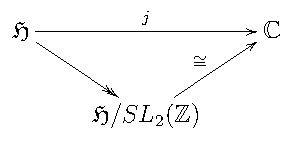
\includegraphics[width=0.2351\paperwidth]{images/L8-p061-j.pdf}\end{figure}
对任意有限指数子群$\Gamma\subset\SL_2(\Z)$，令$Y_\Gamma:=\mathcal H/\Gamma$，它是一维复解析流形。记$X_\Gamma$为$Y_\Gamma$的紧化\znote{「紧化」指把非紧的$Y_\Gamma$补成一个紧的对象。这里只需补上有限多个尖点，得到紧Riemann面，它同时是$\Q$上的光滑射影曲线。对一般的复流形，紧化并不唯一、往往要作额外选择；但在曲线情形，光滑紧化由$Y_\Gamma$唯一决定，所以「紧化」在这里没有歧义。[来源：nLab "compactification"，\url{https://ncatlab.org/nlab/show/compactification}（Last revised 2025-08-19；2026-11-14 访问）。]}，
\sourcepage{62}
则有
\begin{figure}[H]\centering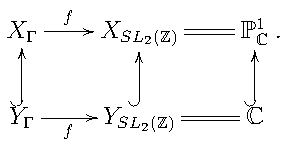
\includegraphics[width=0.2303\paperwidth]{images/L8-p062-compactification.pdf}\end{figure}
$X_\Gamma$是一条光滑射影曲线，并且$X_\Gamma\cong(\mathcal H\cup\mathbb P^1(\Q))/\Gamma$。由Riemann--Hurwitz公式，有
\begin{equation}\tag{1.1}\label{L8eq11}
2-2g(X_\Gamma)=2\deg f-\sum_P(e_P-1),
\end{equation}
其中$g(X_\Gamma)$为$X_\Gamma$的算术亏格，求和遍历$f$的所有分歧点$P\in X_\Gamma$，$e_P$为相应分歧指数。

本讲主要考虑下列两类同余子群：
\begin{align*}
\Gamma_1(N)&:=\left\{\begin{pmatrix}a&b\\c&d\end{pmatrix}\in\SL_2(\Z)\ \middle|\ a\equiv1,\ c\equiv0\pmod N\right\}\\
&\subset\Gamma_0(N):=\left\{\begin{pmatrix}a&b\\c&d\end{pmatrix}\in\SL_2(\Z)\ \middle|\ c\equiv0\pmod N\right\}.
\end{align*}
此前已经见过Hecke同余子群$\Gamma_0(N)$。映射$\begin{pmatrix}a&b\\c&d\end{pmatrix}\mapsto d\bmod N$将商$\Gamma_0(N)/\Gamma_1(N)$与$(\Z/N\Z)^\times$等同。它们的指数分别为
\[[\SL_2(\Z):\Gamma_0(N)]=N\prod_{p\mid N}(1+p^{-1}),\qquad [\SL_2(\Z):\Gamma_1(N)]=N^2\prod_{p\mid N}(1-p^{-2}).\]
对$j=0,1$，定义$Y_j(N):=Y_{\Gamma_j(N)}$，$X_j(N):=X_{\Gamma_j(N)}$。模曲线\znote{「模曲线」中的「模」指 moduli，即参数空间：这类曲线本来是用来参数化带附加结构的椭圆曲线的，而不是先有曲线再去找参数。作为复解析空间它是$\mathcal H/\Gamma$，作为代数对象它是$\Q$上的一维概形，两种描述的一致性由GAGA给出。模形式则是模曲线上的微分形式，二者是同源词。[来源：nLab "modular curve"，\url{https://ncatlab.org/nlab/show/modular+curve}（Last revised 2015-07-21；2026-11-14 访问）。]}$Y_1(N)$有如下解释：
\[Y_1(N)\ \xleftrightarrow{\;1\text{--}1\;}\ \left\{\begin{array}{l}\text{二元组$(E,P)$的同构类，其中$E$为$\C$上的椭圆曲线，}\\\text{$P\in E(\C)$为阶恰等于$N$的点。}\end{array}\right\}.
\]
\sourcepage{63}
这一双射由下列映射诱导：
\begin{equation}\tag{1.2}\label{L8eq12}
g_1:\tau\longmapsto\left(E=\C/(\Z\oplus\tau\Z),\quad P\equiv\frac1N\pmod{\Z\oplus\tau\Z}\right).
\end{equation}
\begin{exercise*}\label{L8S1EX1}
验证\eqref{L8eq12}中的$g_1$在$\Gamma_1(N)$作用下不变。

需注意：对于$\gamma=\begin{pmatrix}a&b\\c&d\end{pmatrix}\in\Gamma_1(N)$，有$\gamma(\tau)=(a\tau+b)/(c\tau+d)$，并且
\[(a\tau+b)\Z\oplus(c\tau+d)\Z=\Z\oplus\tau\Z\]
与$\Z\oplus\gamma(\tau)\Z$位似。因此，还要证明在乘以$c\tau+d$所给出的同构下，标记点满足
\[\frac1{N\gamma(\tau)}(a\tau+b)=\frac{c\tau+d}{N}\equiv\frac1N\pmod{\Z\oplus\tau\Z}.\]
\end{exercise*}
同样，有
\[Y_0(N)\ \xleftrightarrow{\;1\text{--}1\;}\ \left\{\begin{array}{l}\text{二元组$(E,G)$的同构类，其中$E$为$\C$上的椭圆曲线，}\\\text{$G\subset E(\C)$为阶$N$的循环子群。}\end{array}\right\}.\]
现在尝试在这些模曲线上构造通用族：
\begin{figure}[H]\centering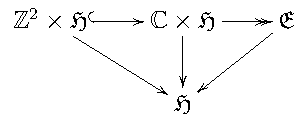
\includegraphics[width=0.2458\paperwidth]{images/L8-p063-family.pdf}\end{figure}
设$z$、$\tau$分别为$\C$、$\mathcal H$上的复坐标。群$\SL_2(\Z)$通过
\[\gamma\cdot(z,\tau)=\left(\frac z{c\tau+d},\gamma(\tau)\right),\qquad\gamma=\begin{pmatrix}a&b\\c&d\end{pmatrix},\]
作用于族$\mathcal E$。存在自然的零截面$0:\mathcal H\to\mathcal E$，它在每条看作加法群的曲线上选取零元。定义$\omega:=0^*\Omega^1_{\mathcal E/\mathcal H}$，则$\omega$由$dz$生成。对$\gamma\in\SL_2(\Z)$，有
\[\gamma^*dz=\frac1{c\tau+d}dz,\qquad \gamma^*\bigl(f(dz)^{\otimes k}\bigr)=(\gamma\cdot f)(c\tau+d)^{-k}(dz)^{\otimes k}.\]
因此，若$\Gamma$是$\SL_2(\Z)$的任意同余子群，$f\in M_k(\Gamma)$，则$f(dz)^{\otimes k}$是$\Gamma$不变的。可以把$M_k(\Gamma)$看成$H^0(\mathcal H,\omega^{\otimes k})$中在所有尖点处正则的$\Gamma$不变截面组成的子空间。此外，若
\sourcepage{64}
$\Gamma$在$\mathcal H$上的作用足够好，例如为自由作用，则$\omega$下降为$Y_\Gamma$上的线丛$\omega_Y$。若$\Gamma$进一步在尖点处正则作用，即
\[\Gamma_\infty\subset\left\{\begin{pmatrix}1&*\\0&1\end{pmatrix}\right\},\qquad \gamma\Gamma_c\gamma^{-1}\subset\left\{\begin{pmatrix}1&*\\0&1\end{pmatrix}\right\}\quad(\gamma c=\infty),\]
则要求$\omega_Y$的生成截面在尖点处的阶为0，便可以将它延拓到$X_\Gamma$。略微混用记号，将$\mathcal H$、$Y_\Gamma$和$X_\Gamma$上的这个线丛都记为$\omega$。有
\[M_k(\Gamma)=H^0(X_\Gamma,\omega^{\otimes k}).\]
另一方面，由形变理论，Kodaira--Spencer映射给出同构$R^1\pi_*T_{\mathcal E/\mathcal H}\cong T_{\mathcal H}$，其中$\pi:\mathcal E\to\mathcal H$为投影，$T_{\mathcal E/\mathcal H}$为$\pi$的相对切丛，$T_{\mathcal H}$为$\mathcal H$上的切丛。由凝聚对偶性——Serre对偶性的推广——得到
\begin{equation}\tag{1.3}\label{L8eq13}
\begin{aligned}
\Omega^1_{\mathcal H}&\cong(R^1\pi_*T_{\mathcal E/\mathcal H})^\vee
\cong\pi_*(\Omega^1_{\mathcal E/\mathcal H}\otimes T_{\mathcal E/\mathcal H}^\vee)\\
&\cong\pi_*((\Omega^1_{\mathcal E/\mathcal H})^{\otimes2})
\cong(0^*\Omega^1_{\mathcal E/\mathcal H})^{\otimes2}=\omega^{\otimes2}.
\end{aligned}
\end{equation}
\begin{exercise*}\label{L8S1EX2}
证明$\pi_*((\Omega^1_{\mathcal E/\mathcal H})^{\otimes2})\cong0^*((\Omega^1_{\mathcal E/\mathcal H})^{\otimes2})$。

提示：注意，$0(\mathcal H)$是$\mathcal E$中的一个除子。使用正合列
\[0\to\OO_{\mathcal E}(-0(\mathcal H))\to\OO_{\mathcal E}\to\OO_{0(\mathcal H)}\to0,\]
并证明$\pi_*((\Omega^1_{\mathcal E/\mathcal H})^{\otimes2}(-0(\mathcal H)))=0$，且$R^1\pi_*((\Omega^1_{\mathcal E/\mathcal H})^{\otimes2}(-0(\mathcal H)))$局部自由。
\end{exercise*}
由\eqref{L8eq13}，$\omega^{\otimes2}\cong\Omega^1_{Y_\Gamma}$，于是$(dz)^{\otimes2}$对应于$d\tau$。
% [Tutor Note: 原书 p64 作 "By (1.3), we have $\omega\cong\Omega^1_{Y_\Gamma}$"，与 \eqref{L8eq13} 的量纲不符，应为 $\omega^{\otimes2}\cong\Omega^1_{Y_\Gamma}$，译文按正确写法处理。]
\originalnumber{2}
\begin{note}[L8S1O2]
对任意$\gamma=\begin{pmatrix}a&b\\c&d\end{pmatrix}$，也可以直接看出
\[\gamma^*(dz)^{\otimes2}=\frac{(dz)^{\otimes2}}{(c\tau+d)^2},\qquad \gamma^*(d\tau)=\frac{d\tau}{(c\tau+d)^2},\]
这与$(dz)^{\otimes2}$对应于$d\tau$相容。
\end{note}
将$\omega$延拓到$X_\Gamma$时，在尖点处取局部参数$q$，有$d\tau$为$dq/q$的非零常数倍。因此，当$f\in S_2(\Gamma)$时，$f(dz)^{\otimes2}$给出$\Omega^1_{X_\Gamma}$的截面。一般地，得到
\[S_k(\Gamma)=H^0(X_\Gamma,\omega^{\otimes(k-2)}\otimes\Omega^1_{X_\Gamma}).\]
\sourcepage{65}
当$N\geq5$时，$\Gamma_1(N)$在$\mathcal H$上自由作用，且在尖点处正则；而$\Gamma_0(N)$的作用从来不是自由的，也不满足上述尖点正则条件。为从尖点模形式构造Galois表示，下面使用$X_1(N)$，并从现在起假定$N\geq5$。对$N\leq4$，也仍可以通过相应的模函子\znote{「模空间」是参数空间的正式说法：它的点与所参数化对象（这里是带水平结构的椭圆曲线）的同构类一一对应。严格的定义要用「模函子」，即把每个概形$S$映到「$S$上这类对象族」的集合。当对象带有非平凡自同构时，细模空间往往不存在，只能用粗模空间或模函子来代替；上一句提到的$N\leq4$正是这种情况。[来源：nLab "moduli space"，\url{https://ncatlab.org/nlab/show/moduli+space}（Last revised 2025-10-21；2026-11-14 访问）。]}完成整个构造，而不是直接使用这些模曲线。
\begin{exercise*}\label{L8S1EX3}
证明：$\Gamma_1(N)$在$\mathcal H$上自由作用，当且仅当$N\geq4$。

提示：先证明：对$\SL_2(\R)$中的非标量矩阵$\begin{pmatrix}a&b\\c&d\end{pmatrix}$，存在$\tau\in\mathcal H$满足$(a\tau+b)/(c\tau+d)=\tau$，当且仅当$(a+d)^2<4$。
\end{exercise*}
通用族$\mathcal E$也诱导$Y_1(N)$上的通用族$\mathcal E_Y$。它的半阿贝尔延拓的单位连通分支给出$X_1(N)$上的光滑群概形$\mathcal E_X$；尖点处的纤维同构于$\C^\times$。其原因是，当$\tau$趋向尖点$\infty$时，格$\Z\oplus\tau\Z$退化为秩1的格，因而尖点处的纤维为$\C/\Z\cong\C^\times$。
\section{Hecke算子与Hecke代数}\label{L8S2}\idx{Hecke算子}\idx{菱形算子}
由于$\Gamma_1(N)$是$\Gamma_0(N)$的正规子群，$\Gamma_0(N)$自然通过
\[f\longmapsto\gamma_k^*f(\tau):=(c\tau+d)^{-k}f(\gamma(\tau)),\qquad \gamma=\begin{pmatrix}a&b\\c&d\end{pmatrix}\in\Gamma_0(N),\]
作用于$S_k(\Gamma_1(N))$。$\Gamma_1(N)$在这一空间上的作用平凡，因此该作用下降为$\Gamma_0(N)/\Gamma_1(N)\cong(\Z/N\Z)^\times$的作用。对于$d\in(\Z/N\Z)^\times$，将其作用记为$\langle d\rangle$，称为\textbf{菱形算子}。也就是说，对任意右下角模$N$等于$d$的$\gamma\in\Gamma_0(N)$，都有$\langle d\rangle f=\gamma_k^*f$。由于$(\Z/N\Z)^\times$为交换群，有按特征标的分解
\[S_k(\Gamma_1(N))=\bigoplus_{\chi:(\Z/N\Z)^\times\to\C^\times}S_k(N,\chi),\]
其中$S_k(N,\chi)$与\lref{L6}的定义相同。此外，$S_k(N)=S_k(N,1)=S_k(\Gamma_1(N))^{\Gamma_0(N)}$。

Hecke代数\znote{Hecke代数可以理解为「所有Hecke算子一起生成的代数」：它作用在$S_k(\Gamma_1(N))$上，使后者成为它的模，而同时对角化就得到特征形式。在双陪集的语言里，它由$\Gamma\backslash\Delta/\Gamma$生成，乘法由双陪集的分解决定；对$\Gamma_1(N)$这个代数交换，这正是Hecke理论能继续做下去的关键。[来源：F. Diamond and J. Shurman, \textit{A First course in Modular forms}, Springer GTM 228 (2005), Section 7.9（本讲参考文献）。]}
\[\mathcal H_k(\Gamma_1(N)):=\Q[T_n\ (n\geq1),\ \langle d\rangle\ (d\in(\Z/N\Z)^\times)]\subset\End(S_k(\Gamma_1(N)))\]
是有限维交换$\Q$代数，其中$T_n$为Hecke算子。
\sourcepage{66}
这些算子形式地满足关系
\begin{equation}\tag{2.1}\label{L8eq21}
\sum_{n=1}^\infty T_n n^{-s}=\prod_{p\nmid N}(1-T_pp^{-s}+\langle p\rangle p^{k-1-2s})^{-1}\prod_{p\mid N}(1-T_pp^{-s})^{-1}.
\end{equation}
% [Tutor Note: 原书 p66 式 (2.1) 的第一个乘积下标也印作 $p\mid N$，与第二个相同；第一个应为 $p\nmid N$（否则不再是标准的 Euler 乘积，也与注 2.4 中 $L_f(s)$ 的展开不符）。原书 p68 的 $L_f(s)$ 展开同样如此。译文按 $p\nmid N$ 处理。]
下面定义$T_n$。对整数$N\geq4$、$n\geq1$，存在$Y_1(N)$上的有限平坦概形$T_1(N,n)$，其点可解释为如下三元组的同构类：
\[\left\{\begin{array}{l}(E,P,G),\quad\text{其中$E$为椭圆曲线，$P$为$E$上阶$N$的点，}\\\text{$G\subset E$为阶$n$的有限子群，且$G\cap\langle P\rangle=0$。}\end{array}\right\}.\]
自然的遗忘态射$s_Y:T_1(N,n)\to Y_1(N)$由$s_Y(E,P,G)=(E,P)$给出。另一个态射$t_Y:T_1(N,n)\to Y_1(N)$定义为$t_Y(E,P,G)=(E/G,\overline P)$。由于$\langle P\rangle\cap G=0$，$P$在$E/G$中的像$\overline P$仍然具有阶$N$。$s_Y,t_Y$都唯一延拓为完备正规曲线之间的有限平坦态射$s,t:\overline T_1(N,n)\to X_1(N)$：
\begin{figure}[H]\centering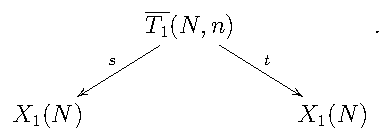
\includegraphics[width=0.3131\paperwidth]{images/L8-p066-correspondence.pdf}\end{figure}
于是有拉回及迹映射
\begin{align*}
t^*:S_k(\Gamma_1(N))&=H^0(X_1(N),\omega^{\otimes(k-2)}\otimes\Omega^1)\\
&\longrightarrow H^0(\overline T_1(N,n),t^*\omega^{\otimes(k-2)}\otimes\Omega^1),\\
s_*:H^0(\overline T_1(N,n),s^*\omega^{\otimes(k-2)}\otimes\Omega^1)&\longrightarrow H^0(X_1(N),\omega^{\otimes(k-2)}\otimes\Omega^1)\\
&=S_k(\Gamma_1(N)).
\end{align*}
由于$s,t$都是有限平坦映射，有$s_*\Omega^1\cong t_*\Omega^1\cong\Omega^1$。这里略微混用记号，$\Omega^1$始终表示相应曲线的余切丛；通过有限映射的微分拉回和迹映射定义上述箭头。存在通用同源$\nu:\mathcal E_T\twoheadrightarrow\mathcal E'_T$，其在$x=(E,P,G)\in T_1(N,n)$处的纤维为$E\twoheadrightarrow E/G$。有下列交换图；基底上的箭头为恒等映射：
\begin{figure}[H]\centering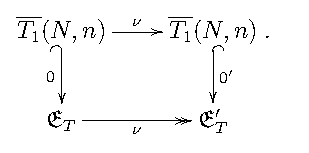
\includegraphics[width=0.2495\paperwidth]{images/L8-p066-isogeny.pdf}\end{figure}
\sourcepage{67}
由线丛$\omega$的函子性，在$T_1(N,n)$上有$t^*\omega\cong0'^*\Omega^1_{\mathcal E'_T/T}$及$s^*\omega\cong0^*\Omega^1_{\mathcal E_T/T}$。在特征0中，有限平坦的同源$\nu$在相对微分上诱导同构$\nu^*\Omega^1_{\mathcal E'_T/T}\cong\Omega^1_{\mathcal E_T/T}$，因而$\nu^*t^*\omega\cong s^*\omega$。有自然映射
\begin{figure}[H]\centering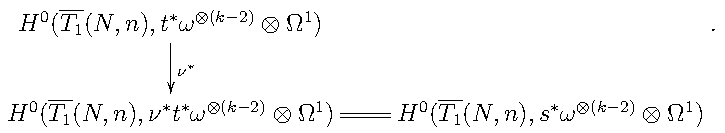
\includegraphics[width=0.5842\paperwidth]{images/L8-p067-pullback.pdf}\end{figure}
定义Hecke算子$T_n=s_*\circ\nu^*\circ t^*$\znote{这里用对应（correspondence）定义$T_n$，经典的说法则是双陪集：$T_n$对应双陪集$\Gamma\begin{pmatrix}1&0\\0&n\end{pmatrix}\Gamma$，把它分解为$\bigsqcup_i\Gamma\alpha_i$后，作用就是$f\mapsto\sum_i f|_k\alpha_i$。两种说法等价：对应的两个投影$s,t$正是双陪集各分支的「来源」与「去向」。用对应来写的好处是它对任意概形都说得通。[来源：nLab "double coset"，\url{https://ncatlab.org/nlab/show/double+coset}（Last revised 2019-08-01；2026-11-14 访问）。]}，使下图交换：
\begin{figure}[H]\centering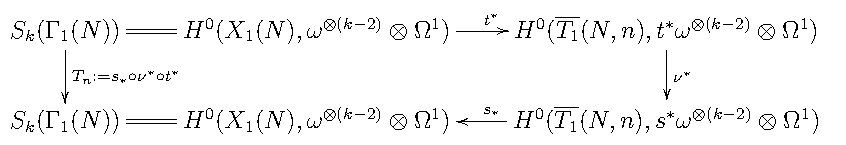
\includegraphics[width=0.6818\paperwidth]{images/L8-p067-Hecke.pdf}\end{figure}
\originalnumber{1}
\begin{note}[L8S2O1]
当$n=p$为素数时，Hecke算子$T_p$可以显式定义为：对任意$f\in S_k(\Gamma_1(N))$，
\[T_pf(\tau)=\frac1p\sum_{j=0}^{p-1}f\left(\frac{\tau+j}p\right)+\begin{cases}p^{k-1}(\langle p\rangle f)(p\tau),&p\nmid N,\\0,&p\mid N.\end{cases}\]
以$q$展开$f(\tau)=\sum_na_n(f)q^n$表示，有
\[T_pf(\tau)=\sum_{p\mid n}a_n(f)q^{n/p}+\begin{cases}p^{k-1}\sum_na_n(\langle p\rangle f)q^{pn},&p\nmid N,\\0,&p\mid N.\end{cases}\]
% [Tutor Note: 原书 p67 此式第一个求和的指标印作 $p\mid N$，应为 $p\mid n$（求和跑遍被 $p$ 整除的 $n$），译文按正确写法处理。]
\end{note}
\originalnumber{2}
\begin{note}[L8S2O2]
当$N\leq3$时，只有模函子$T_1(N,n):(\mathrm{Schemes})\to(\mathrm{Sets})$。此时需要处理函子间的态射，而非概形间的态射，但本质上并无额外的技术困难。
\end{note}
\originalnumber{3}
\begin{definition}{归一化特征形式}\label{L8S2O3}
若尖点形式$f=\sum_{n=1}^\infty a_nq^n\in S_k(N,\chi)$是所有$T_n$的特征向量，且$a_1=1$，就称它为\textbf{归一化特征形式}。
\end{definition}
\originalnumber{4}
\begin{note}[L8S2O4]
若$f$为归一化特征形式，则$a_1(T_nf)=a_n(f)$。由于Hecke代数为有限维$\Q$代数，子域$\Q(f):=\Q(a_1(f),a_2(f),\ldots)\subset\C$是
\sourcepage{68}
$\Q$的有限扩张。此外，由\eqref{L8eq21}，有
\begin{align*}
L_f(s)&=\sum_{n=1}^\infty a_n(f)n^{-s}=\sum_{n=1}^\infty a_1(T_nf)n^{-s}\\
&=\prod_{p\nmid N}(1-a_1(T_pf)p^{-s}+a_1(\langle p\rangle f)p^{k-1-2s})^{-1}\\
&\hspace{1em}\cdot\prod_{p\mid N}(1-a_1(T_pf)p^{-s})^{-1}\\
&=\prod_{p\nmid N}(1-a_pp^{-s}+\chi(p)p^{k-1-2s})^{-1}\prod_{p\mid N}(1-a_pp^{-s})^{-1}.
\end{align*}
\end{note}
\originalnumber{5}
\begin{proposition}\label{L8S2O5}
映射
\[e:S_k(\Gamma_1(N))\longrightarrow\Hom_{\Q}(\mathcal H_k(\Gamma_1(N)),\C),\qquad f\longmapsto\bigl(T\mapsto a_1(Tf)\bigr),\]
是$\Q$向量空间同构。此外，$e$诱导有限集之间的双射
\[\{f\in S_k(\Gamma_1(N))\mid f\text{为归一化特征形式}\}\xrightarrow{\;1\text{--}1\;}\Hom_{\Q\text{-代数}}(\mathcal H_k(\Gamma_1(N)),\C).\]
\end{proposition}
下面的定理将帮助确定所构造的Galois表示在哪些素位处非分歧。
\originalnumber{6}
\begin{theorem}{Igusa}\label{L8S2O6}
当$N\geq4$时，$Y_1(N)$和$X_1(N)$在$\Z[1/N]$上都具有良约化。
\end{theorem}
Eichler--Shimura、Deligne主定理在$k=1$时的结论由Deligne与Serre证明。这时，$\sigma_{f,\ell}$有有限像，相应的复表示与$\ell$无关。这些表示不能用$k\geq2$时同样的方式构造。下面只考察$k\geq2$的情形。
\section{权\texorpdfstring{$k=2$}{k=2}时的主定理}\label{L8S3}\idx{Jacobian簇}
此时，$S_2(\Gamma_1(N))\cong H^0(X_1(N),\Omega^1)$。记$J_1(N)$为参数化曲线$X_1(N)$上次数0线丛的Jacobian簇\znote{「Jacobian簇」把曲线的参数化问题线性化：$J(X)$的点就是$X$上的次数$0$线丛，$P\mapsto\OO(P-P_0)$把$X$嵌入$J(X)$。它既是$g$维阿贝尔簇，又是复环面$H^0(X,\Omega^1)^\vee/H_1(X,\Z)$，两种结构的相容性正是Hodge理论的内容。名称来自Jacobi对椭圆积分的研究：当$X$本身是椭圆曲线时$J(X)\cong X$，椭圆曲线上的群结构正由此而来。[来源：nLab "Jacobian variety"，\url{https://ncatlab.org/nlab/show/Jacobian+variety}（Last revised 2026-09-26；2026-11-14 访问）。]}。则
\[J_1(N)\cong H^0(X_1(N),\Omega^1)^\vee/H_1(X_1(N),\Z).\]
\originalnumber{1}
\begin{note}[L8S3O1]
一般地，对紧复Kähler流形$X$，其Picard环面
\sourcepage{69}
为$\operatorname{Pic}^0(X)\cong H^1(X,\OO_X)/H^1(X,\Z)$，而
\[\operatorname{Alb}(X):=H^0(X,\Omega^1)^\vee/H_1(X,\Z)\]
称为Albanese环面，当$X$为曲线时，由Poincaré对偶性及Hodge理论，$H^1(X,\Z)\cong H_1(X,\Z)$，$H^0(X,\Omega^1)^\vee\cong H^1(X,\OO_X)$；此时Picard环面与Albanese环面同构。一般情形中，它们只是互为对偶。
\end{note}
$J_1(N)$是阿贝尔簇，其Tate模为
\[T_\ell J_1(N)=\varprojlim_n J_1(N)[\ell^n](\overline{\Q})\cong\Z_\ell^{2g}.\]
如上一讲所述，$T_\ell J_1(N)$给出$\Gal(\overline{\Q}/\Q)$的一个维数$2g(X_1(N))$的$\ell$进表示。由\eref{定理}{L8S2O6}，$X_1(N)$在所有$p\nmid N$处具有良约化，$J_1(N)$亦然。因此，$T_\ell J_1(N)$在$p\nmid\ell N$处非分歧。

若$g(X_1(N))=1$，例如$N=11$，则$T_\ell J_1(N)\otimes\Q_\ell$已经是二维Galois表示。一般地，若$g(X_1(N))\ne1$，则需要通过与模形式$f$相应的特征值特化映射$e_f:\mathcal H_2(\Gamma_1(N))\to\Q(f)$，从$T_\ell J_1(N)$中提取二维Galois表示。注意，存在Hodge分解
\[H^1(X_1(N),\C)\cong H^0(X_1(N),\Omega^1)\oplus H^1(X_1(N),\OO_{X_1(N)}).\]
因此有以下命题。
\originalnumber{2}
\begin{proposition}\label{L8S3O2}
下面的映射，是$\mathcal H_2(\Gamma_1(N))\otimes_{\Q}\R$模同构：
\begin{figure}[H]\centering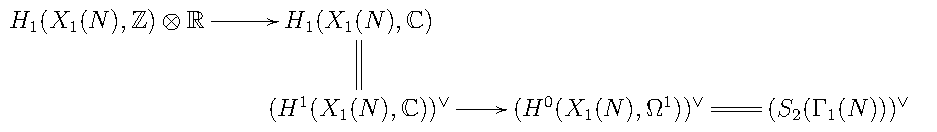
\includegraphics[width=0.7556\paperwidth]{images/L8-p069-homology.pdf}\end{figure}
\end{proposition}
结合\eref{命题}{L8S2O5}与\eref{命题}{L8S3O2}，得到$H_1(X_1(N),\Q)$是$\mathcal H_2(\Gamma_1(N))$上的秩2模。因此，$T_\ell J_1(N)\otimes\Q_\ell$是$\mathcal H_2(\Gamma_1(N))\otimes\Q_\ell$上的秩2自由模。取归一化特征形式$f\in S_2(N,\chi)$，设
\sourcepage{70}
$\lambda$为$\Q(f)$中位于$\ell$上方的素位。存在$\Q$代数同态
\[e_f:\mathcal H_2(\Gamma_1(N))\to\Q(f),\qquad T_n\mapsto a_n(f),\quad\langle d\rangle\mapsto\chi(d).\]
定义
\[V_{f,\lambda}:=(T_\ell J_1(N)\otimes_{\Z_\ell}\Q_\ell)\otimes_{\mathcal H_2(\Gamma_1(N))\otimes\Q_\ell}\Q(f)_\lambda.\]
则$V_{f,\lambda}$是$\Gal(\overline{\Q}/\Q)$在二维$\Q(f)_\lambda$向量空间上的$\ell$进表示，且在$p\nmid\ell N$处非分歧。
\originalnumber{3}
\begin{theorem}\label{L8S3O3}
$\ell$进表示$\sigma_{f,\lambda}:\Gal(\overline{\Q}/\Q)\to\GL(V_{f,\lambda})$与$f$相联系；也就是说，对$p\nmid N\ell$，有
\[\det(1-t\sigma_{f,\lambda}(\mathrm{Fr}_p))=1-a_p(f)t+\chi(p)pt^2.\]
\end{theorem}
若对所有$n\geq1$都有$a_n(f)\in\Z$，则$e_f$将整Hecke代数$\mathcal H_2(\Gamma_1(N))_{\Z}:=\Z[T_n;\langle d\rangle]$满射到$\Z$。因此，存在将$H_1(X_1(N),\Z)$映到$\C$中某个秩2格$\Lambda_f$的映射。由此得到定义在$\Q$上的椭圆曲线$E_f$，并且$\Q(f)=\Q$、$V_{f,\lambda}\cong T_\ell E_f\otimes\Q_\ell$。下面的定理加强了\eref{定理}{L7S2O9}。
\originalnumber{4}
\begin{theorem}{Shimura--Taniyama--Weil猜想}\label{L8S3O4}
每条$\Q$上的椭圆曲线$E$都与某条$E_f$同源，其中$f$是权2、级$N_E$的新形式\znote{「新形式」是相对于「旧形式」而言的：若$f\in S_k(N)$来自更小级数的模形式，即形如$g(mz)$（$m>1$），它就是旧形式；新形式指新子空间（旧形式的正交补）中的归一化特征形式。由重数一性质，归一化特征形式由它的Fourier系数唯一确定，因此「级$N_E$的新形式」与椭圆曲线$E$的对应是唯一确定的。[来源：F. Diamond and J. Shurman, \textit{A First course in Modular forms}, Springer GTM 228 (2005), Chapter 9（本讲参考文献）。]}，$N_E$为$E$的导子。
\end{theorem}
\section{权\texorpdfstring{$k>2$}{k>2}时的主定理}\label{L8S4}
这里只陈述结果，其形式与$k=2$时类似。设$\pi:\mathcal E_Y\to Y_1(N)$为通用族，$j:Y_1(N)\hookrightarrow X_1(N)$为开浸入。
\originalnumber{1}
\begin{proposition}\label{L8S4O1}
存在$\mathcal H_k(\Gamma_1(N))\otimes_{\Q}\R$模的典范同构
% [Tutor Note: 原书 p70 命题 4.1 把 Hecke 代数记作 $T_k(\Gamma_1(N))$，与算子记号 $T_n$ 冲突，应为 $H_k$（即本译本的 $\mathcal H_k$），译文按正确记号处理。]
\[H^1(X_1(N)(\C),j_*\operatorname{Sym}^{k-2}R^1\pi_*\Q)\otimes_{\Q}\R\xrightarrow{\sim}S_k(\Gamma_1(N)).\]
因此，左边的有理上同调空间是$\mathcal H_k(\Gamma_1(N))$上的秩2自由模。
\end{proposition}
取归一化特征形式$f\in S_k(N,\chi)$。对$\Q(f)$中位于$\ell$上方的素位$\lambda$，定义
\[\begin{aligned}
V_{f,\lambda}:={}&H^1_{\mathrm{ét}}(X_1(N)_{\overline{\Q}},j_*\operatorname{Sym}^{k-2}R^1\pi_*\Q_\ell)\\
&\otimes_{\mathcal H_k(\Gamma_1(N))\otimes\Q_\ell}\Q(f)_\lambda.
\end{aligned}\]
\sourcepage{71}
则$V_{f,\lambda}$为$\Gal(\overline{\Q}/\Q)$的二维$\ell$进表示，并在$p\nmid\ell N$处非分歧。
\originalnumber{2}
\begin{theorem}\label{L8S4O2}
$\ell$进表示$\sigma_{f,\lambda}:\Gal(\overline{\Q}/\Q)\to\GL(V_{f,\lambda})$的对偶与$f$相联系；也就是说，对$p\nmid N\ell$，有
\[\det(1-t\sigma_{f,\lambda}^*(\mathrm{Fr}_p))=1-a_p(f)t+\chi(p)p^{k-1}t^2.\]
\end{theorem}
\originalnumber{3}
\begin{note}[L8S4O3]
\eref{定理}{L8S4O2}中取对偶是自然的，因为这里使用的是上同调群；而在$k=2$时，一开始就通过使用同调群而非上同调群取了对偶。
\end{note}
\needspace{5\baselineskip}\section{第8讲参考文献}\label{L8S5}
\needspace{4\baselineskip}\textbf{关于Hecke算子。}
\begin{references}
\refitem{L8bibDS7}{DS} F. Diamond and J. Shurman, \emph{A First course in Modular forms}, Springer GTM 228 (2005), Section 7.9
% [Tutor Note: 原书 p71 此条作者名印作 "J. Churman"，应为 J. Shurman，译文按正确拼写处理。]
\end{references}
\needspace{4\baselineskip}\textbf{关于$Y_1(N)$与$X_1(N)$在$\Z[1/N]$上的约化。}
\begin{references}
\refitem{L8bibDR}{DR} P. Deligne and M. Rapoport, \emph{Les schémas de modules de courbes elliptique}, in W. Kuyk, P. Deligne (eds.) Modular Functions of One Variable II, Lecture Notes in Math., Springer, 349, 1973, 143-316.
% [Tutor Note: 原书 p71 此条作者名印作 "M. Papoport"，应为 M. Rapoport，译文按正确拼写处理。]
\end{references}
\needspace{4\baselineskip}\textbf{关于权$k=2$时Galois表示的构造。}
\begin{references}
\refitem{L8bibDS9}{DS} F. Diamond and J. Shurman, \emph{A First course in Modular forms}, Springer GTM 228 (2005), Chapter 9.
% [Tutor Note: 原书 p71 此条作者名印作 "J. Churman"，应为 J. Shurman，译文按正确拼写处理。]
\refitem{L8bibLW}{LW} D. Loeffler and J. Weinstein, \emph{On the computation of local components of a newform}, In: Math. Comp. 81. 278 (2012), pp. 1179-1200.
\end{references}
\needspace{4\baselineskip}\textbf{关于权$k>2$的情形。}
\begin{references}
\refitem{L8bibD}{D} P. Deligne, \emph{Forms modulaires et représentations $\ell$-adiques}, Séminaire Bourbaki no 355, in Lecture Notes in Math., Springer, 179, 1971, 139-172.
\end{references}

\chapter{从数域到函数域}\label{L9}\lecturedate{2020/03/16}\sourcepage{72}
本讲介绍函数域的Langlands对应。
\section{作为整体域的函数域}\label{L9S1}
整数环与域$k$上的一元多项式环$k[t]$有许多相似之处。$\Z$中的素数对应于$k[t]$中的不可约多项式。如前所述，每个素数$p$可以看作$\Q$上的一个赋值；类似地，每个不可约多项式$r(t)$在分式域$k(t)$上给出赋值
\begin{equation}\tag{1.1}\label{L9eq11}
\left|r(t)^a\frac{u(t)}{v(t)}\right|_r=c^{-a},
\end{equation}
其中$c>1$固定，$u(t),v(t)\in k[t]$，且$r(t)\nmid u(t)$、$r(t)\nmid v(t)$。

对固定的$c>1$，还有赋值$|\cdot|_\infty$，定义为
\begin{equation}\tag{1.2}\label{L9eq12}
\left|\frac{u(t)}{v(t)}\right|_\infty=c^{\deg u-\deg v}.
\end{equation}
虽然$|\cdot|_\infty$不同于每个$|\cdot|_r$，但它们全都是非阿基米德的！与具有阿基米德素位\idx{阿基米德素位}的$\Q$不同，$k(t)$有如下性质。
\originalnumber{1}
\begin{lemma}\label{L9S1O1}
$k(t)$上在$k$上平凡的非平凡赋值，只可能等价于\eqref{L9eq11}或\eqref{L9eq12}中的赋值。特别地，若$k$为有限域，则$k(t)$的所有非平凡赋值都是非阿基米德的。
\end{lemma}
\sourcepage{73}
\begin{proof}
先证明有限域只有平凡赋值。若$k$有限，则对任意$0\ne a\in k$，存在$n\geq1$使$a^n=1$。因此，$1=|1|=|a^n|=|a|^n$，从而$|a|=1$。

设$|\cdot|$为$k(t)$上在$k$上平凡的非平凡赋值。存在不可约多项式$r(t)$，使$|r(t)|\ne1$。选择这样一个次数最小的$r(t)$，便有：对所有非零$d(t)\in k[t]$，若$\deg d<\deg r$，则$|d(t)|=1$。若$\deg r>1$，依假设$|t|=1$。由三角不等式，对任意$g(t)\in k[t]$，有
\[|g(t)|\leq|t^{\deg g}|+\cdots+|1|=\deg g+1.\]
令$g(t)=r(t)^n$，则
\[|r(t)|^n\leq n\deg r+1,\qquad |r(t)|\leq\lim_{n\to\infty}(n\deg r+1)^{1/n}=1.\]
故$R:=|r(t)|<1$。对$r\nmid u$，将$u(t)$写成
\[u(t)=a_m(t)r(t)^m+\cdots+a_0(t),\quad a_0(t)\ne0,\quad\deg a_j<\deg r.\]
由三角不等式，
\[|u(t)|\leq R^m+\cdots+1=\frac{1-R^{m+1}}{1-R}=\frac{1-R^{\lfloor\deg u/\deg r\rfloor+1}}{1-R}.\]
对$u(t)^n$作同样的展开，得到
\[|u(t)|^n=|u(t)^n|\leq\frac{1-R^{\lfloor n\deg u/\deg r\rfloor+1}}{1-R}\leq\frac1{1-R}.\]
令$n\to\infty$，可得$|u(t)|\leq1$。另一方面，
\[1=|a_0(t)^n|\leq|u(t)|^n+R.\]
若$|u(t)|<1$，令$n\to\infty$会得到$1\leq R<1$的矛盾。因此，凡$r\nmid u$都有$|u(t)|=1$，于是$|\cdot|$具有\eqref{L9eq11}的形式，其中$c=1/R$。
% [Tutor Note: 原书 p73 由此处 $1=|a_0(t)^n|\leq|u(t)|^n+R$ 直接断言 $|u(t)|=1$；严格的说法是：若 $|u(t)|<1$，则 $|u(t)|^n\to0$，与 $1\leq|u(t)|^n+R$（其中 $R<1$）矛盾，故 $|u(t)|\geq1$，结合前文的 $|u(t)|\leq1$ 才得到 $|u(t)|=1$。译文补出了这一步。]

若$\deg r=1$，则可写$r(t)=t+a$，$a\in k$。若$|r(t)|<1$，上述展开论证同样给出\eqref{L9eq11}。因此，只需考虑$|r(t)|>1$。对任意$a\ne b\in k$，展开$(t+b+(a-b))^n$得到
\[|t+a|^n\leq\sum_{j=0}^n|t+b|^j,\]
取$n$次方根并令$n\to\infty$，有$|t+a|\leq\max\{|t+b|,1\}$。因$|t+a|>1$，必有$|t+b|>1$，于是$|t+a|\leq|t+b|$。利用$a,b$的对称性，得到$|t+a|=c>1$与$a$无关。证明对任意非零$u(t)\in k[t]$都有$|u(t)|=c^{\deg u(t)}$的方法类似，留给读者。
\end{proof}
\sourcepage{74}
设$k=\F_q$为有限域。对不可约$r(t)$，剩余域$k[t]/(r(t))\cong\F_{q^{\deg r}}$。取$c=q^{\deg r}$时，\eqref{L9eq11}中的赋值称为\textbf{归一化赋值}；\eqref{L9eq12}中的$|\cdot|_\infty$在$c=q$时称为归一化的。

记$K_*$为$k(t)$关于$|\cdot|_*$的完备化，其中$*=r$或$\infty$。注意，$K_\infty\cong k((t^{-1}))$。记$\OO_*$为赋值环。$K_*$上存在不变测度$\mu$，称为Haar测度；它在相差一个乘法常数的意义下唯一。可以通过$\mu(\OO_*)=1$将它归一化。
\originalnumber{2}
\begin{theorem}\label{L9S1O2}
若$|\cdot|_*$为归一化赋值，$\mu$为$K_*$上的归一化Haar测度，则对任意$\alpha,\beta\in K_*$，有$\mu(\alpha+\beta\OO_*)=|\beta|_*$。
\end{theorem}
\begin{proof}
由$\mu$的不变性，只需证明$\mu(\beta\OO_*)=|\beta|_*$。以下设$\beta\ne0$。若$*=r$，写
\[\beta=\sum_{j\geq j_0}a_j(t)r(t)^j,\]
其中$a_j$或者为零，或者$\deg a_j<\deg r$，且$a_{j_0}\ne0$。于是$\beta/r^{j_0}\in\OO_r^\times$，因为$|\beta/r^{j_0}|_r=1$。若$j_0\geq0$，令$S$为次数小于$\deg r$的多项式（包括0）组成的集合，则$|S|=q^{\deg r}$，并且
\[\OO_r=\bigsqcup_{(\alpha_1,\ldots,\alpha_{j_0})\in S^{j_0}}\left(\sum_{l=1}^{j_0}\alpha_l r(t)^{l-1}+\beta\OO_r\right).\]
因此，$\mu(\beta\OO_r)q^{j_0\deg r}=\mu(\OO_r)=1$，从而$\mu(\beta\OO_r)=q^{-j_0\deg r}=|\beta|_r$。

若$j_0<0$，则
\[\beta\OO_r=\bigsqcup_{(\alpha_1,\ldots,\alpha_{-j_0})\in S^{-j_0}}\left(\sum_{l=1}^{-j_0}\alpha_l r(t)^{-l}+\OO_r\right).\]
于是$\mu(\beta\OO_r)=\mu(\OO_r)q^{-j_0\deg r}=q^{-j_0\deg r}=|\beta|_r$。

若$*=\infty$，则$\OO_\infty=\{\sum_{n\geq0}a_nt^{-n}\mid a_n\in k\}$。令$\deg\beta=m_0$，则
\[\begin{aligned}
\OO_\infty&=\bigsqcup_{(\alpha_{m_0+1},\ldots,\alpha_0)\in\F_q^{-m_0}}\left(\sum_{l=m_0+1}^{0}\alpha_l t^l+\beta\OO_\infty\right)&& (m_0\leq0),\\
\beta\OO_\infty&=\bigsqcup_{(\alpha_1,\ldots,\alpha_{m_0})\in\F_q^{m_0}}\left(\sum_{l=1}^{m_0}\alpha_l t^l+\OO_\infty\right)&& (m_0>0).
\end{aligned}\]
两种情形都给出$\mu(\beta\OO_\infty)=q^{m_0}=|\beta|_\infty$，结论得证。
\end{proof}
\sourcepage{75}
我们要研究的函数域比有理函数域$k(t)$稍复杂一些。
\originalnumber{3}
\begin{definition}{曲线的函数域}\label{L9S1O3}
设$X$为有限域$\F_q$上的光滑射影连通曲线。$X$上定义在$\F_q$上的有理函数组成的域$\F_q(X)$，称为$X$的\textbf{函数域}\znote{「函数域」与数域相对：固定有限域$\F_q$后，$\F_q$上一条光滑射影曲线$X$对应一个超越次数为$1$的域$\F_q(X)$，且由$X\mapsto\F_q(X)$可以复原$X$（曲线范畴与函数域范畴反变等价）。与$\Q$的对应关系是：素位对应$X$的闭点（即不可约多项式），整闭包$D_X$对应$\Z$，分式理想对应除子。所以函数域是「几何版的数域」，这正是把它当作整体域来研究的原因。[来源：nLab "function field"，\url{https://ncatlab.org/nlab/show/function+field}（Last revised 2022-06-05；2026-11-14 访问）。]}。
\end{definition}
\originalnumber{4}
\begin{note}[L9S1O4]
函数域$\F_q(X)$是$\F_q(t)$的有限扩张。$\F_q(t)$上的每个赋值只有有限多个延拓到$\F_q(X)$；由下面的\eref{引理}{L9S1O5}，它们都是非阿基米德的。
\end{note}
\originalnumber{5}
\begin{lemma}\label{L9S1O5}
域$K$上的赋值$|\cdot|$为非阿基米德赋值，当且仅当对$K$中由1生成的子环中的所有$n$，都有$|n|\leq1$。特别地，若$\operatorname{char}(K)>0$，则$K$的任何赋值都为非阿基米德赋值。
\end{lemma}
\begin{proof}
按定义，$|\cdot|$非阿基米德，当且仅当$|\alpha+\beta|\leq\max\{|\alpha|,|\beta|\}$。这一条件显然推出$|n|\leq1$。反方向只需证明：若所有$|n|\leq1$，则对任意$0<|\alpha|\leq1$，有$|1+\alpha|\leq1$。由三角不等式，
\[|1+\alpha|^n=|(1+\alpha)^n|\leq\sum_{j=0}^n\left|\binom nj\right||\alpha|^j\leq n+1.\]
故$|1+\alpha|\leq(1+n)^{1/n}$。令$n\to\infty$，得到$|1+\alpha|\leq1$。
\end{proof}
$\F_q[t]$在$\F_q(X)$中的整闭包$D_X$是Dedekind整环。对任意非零素理想$\mathfrak R\subset D_X$，完备化$\F_q(X)_{\mathfrak R}$是$\F_{q^m}((\widetilde t))$的有限扩张，其中$\mathfrak R\cap\F_q[t]=(r(t))$，$r(t)$不可约，$\widetilde t=r(t)$，$m=\deg r(t)$。令$N=[\F_q(X)_{\mathfrak R}:\F_{q^m}((\widetilde t))]$，则作为向量空间，$\F_q(X)_{\mathfrak R}\cong\F_{q^m}((\widetilde t))^{\oplus N}$。每个$\alpha$给出线性变换$m_\alpha:x\mapsto\alpha x$。定义
\[\operatorname{Norm}_{\F_q(X)_{\mathfrak R}/\F_{q^m}((\widetilde t))}(\alpha):=\det m_\alpha\in\F_{q^m}((\widetilde t)).\]
基域上的归一化赋值$|\cdot|_r$唯一延拓到$\F_q(X)_{\mathfrak R}$，为
\[|\alpha|=\left|\operatorname{Norm}_{\F_q(X)_{\mathfrak R}/\F_{q^m}((\widetilde t))}(\alpha)\right|_r^{1/N}.\]
在未完备的整体域情形，有如下定理。
\originalnumber{6}
\begin{theorem}\label{L9S1O6}
设$|\cdot|$为整体域$k$的某个素位\znote{「素位」（place）是数域上「素数」的推广：它指一个绝对值的等价类。它可以来自素数，给出非阿基米德绝对值（如$\Q$上的$p$进绝对值）；也可以来自实嵌入或复嵌入，给出阿基米德绝对值（如$\Q$上通常的绝对值）。用「素位」而不用「素数」，正是为了同时容纳这两类；在函数域情形所有素位都是非阿基米德的，于是素位与曲线上的闭点一一对应。[来源：nLab "place"，\url{https://ncatlab.org/nlab/show/place}（Last revised 2015-12-17；2026-11-14 访问）。]}上的归一化赋值，$K/k$为有限扩张。则
\[\prod_{j=1}^J|\alpha|_j=|\operatorname{Norm}_{K/k}(\alpha)|,\]
\sourcepage{76}
其中$|\cdot|_j$为$|\cdot|$在$K$上的各个延拓所对应的归一化赋值。
\end{theorem}
函数域$F:=\F_q(X)$作为整体域，还具有以下性质：
\begin{itemize}
\item 对任意$\alpha\in F^\times$，只有有限多个归一化赋值满足$|\alpha|>1$；
\item $\prod_*|\alpha|_*=1$，乘积遍历$F$的所有归一化赋值；
\item 相应的弱逼近定理和强逼近定理成立。
\end{itemize}
希望曲线定义在有限域上的另一个原因，是其函数域在素位处完备化后得到局部紧的局部域。
\originalnumber{7}
\begin{theorem}\label{L9S1O7}
设$K$为带有非平凡非阿基米德赋值$|\cdot|$的域。则$K$局部紧，当且仅当以下三个条件成立：
\begin{enumerate}\item $K$完备；\item 剩余域有限；\item 赋值离散。\end{enumerate}
\end{theorem}
\section{自守表示与Galois表示}\label{L9S2}
\textbf{自守表示。}

设$F=\F_q(X)$为函数域。同样可以通过限制直积定义阿代尔环\znote{阿代尔环$\A_F$把所有完备化$F_v$用「限制直积」装在一起：除有限多个分量外，其余分量都落在整数环$\OO_v$里。它比直积小得多（直积太庞大，紧性完全丧失），又比$F$大得多，因此既携带全部局部信息，又是局部紧的。伊代尔群$I_F=\A_F^\times$同理，只是要求每个分量可逆。整体域上的分析、Hecke理论都在$\A_F$上进行，这是「局部—整体原则」的技术载体。[来源：nLab "ring of adeles"，\url{https://ncatlab.org/nlab/show/ring+of+adeles}（Last revised 2025-07-01；2026-11-14 访问）。]}$\A_F$与伊代尔群$I_F$。作为拓扑环，$\A_F$局部紧。$\GL_n(\A_F)$定义为元素取自$\A_F$的可逆$n\times n$矩阵组成的群。其限制直积拓扑使$\GL_n(\A_F)$局部紧，并具有紧开
\sourcepage{77}
子群$K:=\GL_n(\prod_v\OO_v)=\prod_v\GL_n(\OO_v)$。固定$\GL_n(\A_F)$上的Haar测度，使$\mu(K)=1$。令$G=\GL_n$。
\originalnumber{1}
\begin{definition}{尖点自守函数空间}\label{L9S2O1}
设$\mathcal A_0(G,\omega)$为$G(\A_F)$上满足以下条件的所有复值函数$f$组成的空间：
\begin{enumerate}[label=(\roman*)]
\item \textbf{光滑性：}$f$在$G(\A_F)$上局部常值。
\item \textbf{$K$有限性：}$f$的所有右$K$平移张成有限维向量空间，即
\[\dim_{\C}\operatorname{span}_{\C}\{h\cdot f\mid h\in K\}<\infty.\]
\item \textbf{中心特征标：}设$Z(\A_F)$为$G(\A_F)$中的标量矩阵群，且
% [Tutor Note: 原书 p77 作 "the diagonal matrices"，但 $G(\A_F)$ 的中心应为标量矩阵而非全部对角矩阵，译文按标量矩阵处理。]
\[\omega=\prod_v\omega_v:Z(\A_F)\cong\A_F^\times\to\C^\times\]
为在$F^\times$上平凡的特征标。对每个$z\in Z(\A_F)$、$\gamma\in G(F)$，要求$f(z\gamma x)=\omega(z)f(x)$。
\item \textbf{尖点性：}对每个真标准抛物子群$P_{n_1,\ldots,n_s}=M_{n_1,\ldots,n_s}N_{n_1,\ldots,n_s}$，其中$n_1+\cdots+n_s=n$、$s\geq2$，$N$为幂幺根基，积分
\[f_{N_{n_1,\ldots,n_s}}(x):=\int_{N_{n_1,\ldots,n_s}(F)\backslash N_{n_1,\ldots,n_s}(\A_F)}f(gx)\,d\mu(g)\]
作为$G(\A_F)$上的函数恒为零。
\end{enumerate}
\end{definition}
\originalnumber{2}
\begin{note}[L9S2O2]
函数域上定义$\mathcal A(G,\omega)$所需的条件比数域情形少，因为$\A_F$没有来自阿基米德素位的分量。这使我们初步感觉，函数域情形应当比数域情形容易处理。
\end{note}
重数一定理对$\mathcal A_0(G)$同样成立。每个不可约自守表示$\pi$都可以写成限制张量积
\[\pi\cong\bigotimes_{v\in|X|}'\pi_v,\]
其中几乎所有$\pi_v$都是球面表示，即$\pi_v^{G(\OO_v)}\ne0$。在处处非分歧的情形，所有$\pi_v$都是球面的。
\sourcepage{78}
为在局部理论中分类不可约$\pi_v$，同样使用Hecke理论。赋值
\[\pi_v\longmapsto\pi_v^{G(\OO_v)}\]
在$G(F_v)$的不可约球面表示的同构类与Hecke代数$\mathcal H(\GL_n(F_v),\GL_n(\OO_v))$的不可约模之间建立双射。后者可以用$\GL_n(\C)$中的半单共轭类来描述，而$\pi_v^{G(\OO_v)}$也是一维的。

因此，在自守一侧，为每个不可约尖点表示$\pi$赋予一族$\GL_n(\C)$中的半单共轭类：
\[\pi\longleftrightarrow\{\gamma_v\}_{v\text{为非分歧素位}}.\]
这一侧的理论与数域情形类似，只是$\pi$没有来自阿基米德素位的分量。

\textbf{Galois表示。}

注意，$F$不是完美域。这里以$F^{\mathrm{sep}}$表示其可分闭包。设$v$为$F$的一个素位，亦即$X$的一个闭点。$\Gal(F^{\mathrm{sep}}/F)$中有分解子群$D_v$，它在共轭意义下唯一，且同构于$\Gal(F_v^{\mathrm{sep}}/F_v)$。映射$D_v\to\Gal(\overline{k(v)}/k(v))$的核为惯性子群$I_v$。若$I_v\subset\ker\sigma$，称Galois表示$\sigma$在$v$处非分歧。这时，$\mathrm{Fr}_v\in\Gal(\overline{k(v)}/k(v))$给出表示中的良定义共轭类。

再次选择$\overline{\Q}_\ell$向量空间来实现Galois表示，其中$\ell\ne\operatorname{char}(F)$。在处处非分歧的情形，可以把这些表示构造为$X$上的光滑$\ell$进层，亦即局部系统\znote{「局部系统」就是局部常值层：$\Q_\ell$向量空间的局部系统在每个足够小的开集上平凡，粘合数据由基本群（在$\ell$进情形是$\Gal(F^{\mathrm{sep}}/F)$）的表示给出。所以「$\sigma$在处处非分歧」相当于说这个局部系统能延拓到整条$X$上，而不只是某个开子集上。[来源：nLab "local system"，\url{https://ncatlab.org/nlab/show/local+system}（Last revised 2025-04-10；2026-11-14 访问）。]}。因此，对每个这样的$\sigma$，得到一族$\GL_n(\overline{\Q}_\ell)$中的共轭类$\widetilde\sigma_v$。令$\sigma_v$为$\widetilde\sigma_v$的半单部分，即对角矩阵$\operatorname{diag}(\lambda_1(v),\ldots,\lambda_n(v))$的共轭类，其中$\lambda_j(v)$是$\widetilde\sigma_v$的特征值。由下面的定理可见，若几乎所有$v\in|X|$都有$\sigma_{1,v}=\sigma_{2,v}$，则$\sigma_1^{\mathrm{ss}}\cong\sigma_2^{\mathrm{ss}}$；这里$\sigma_j^{\mathrm{ss}}$为$\sigma_j$的半单化。特别地，不可约表示$\sigma$由这族$\{\sigma_v\}$所确定。
\originalnumber{3}
\begin{theorem}{Chebotarev密度定理}\label{L9S2O3}\idx{Chebotarev密度定理}
设$L/F$为整体域的有限Galois扩张，$C\subset\Gal(L/F)$为共轭类。则存在无限多个非分歧素位$\p$，使$\mathrm{Fr}_{\p}$的共轭类为$C$。
\end{theorem}
\sourcepage{79}
\textbf{Langlands对应。}

函数域情形已经是一条定理：$n=2$时由Drinfeld证明，$n>2$时由Lafforgue证明。
\originalnumber{4}
\begin{theorem}\label{L9S2O4}
存在自守表示与Galois表示之间的双射，使
\[\pi\longleftrightarrow\sigma,\qquad\sigma_v=\gamma_v\in\GL_n(\overline{\Q}),\quad\forall v\in|X|.\]
\znote{原书未写出下列条件；以下为文献中的标准表述，供对照，不属原书内容：需固定$\ell\ne\operatorname{char}(F)$及系数域之间的同构$\overline{\Q}_\ell\cong\C$（这两项约定本讲正文已在讨论$\ell$进表示处说明，此处不重复）；$\pi$应取具有有限阶中心特征标的不可约尖点自守表示，$\sigma$应取行列式具有有限阶的不可约连续$n$维$\ell$进Galois表示，且后者几乎处处非分歧。此即Drinfeld（$n=2$）与Lafforgue（$n>2$）的定理。[来源：本讲参考文献 [D] Drinfeld, Amer. J. Math. 105 (1983) 85-114；[L] Lafforgue, Invent. Math. 147 (2002) 1-241。]}
\end{theorem}
\needspace{5\baselineskip}\section{第9讲参考文献}\label{L9S3}
\textbf{一般性介绍。}
\begin{references}
\refitem{L9bibBG}{BG} J. Bernstein and S. Gelbart, eds, \emph{An introduction to the Langlands Program}, Birkhäuser, 2004, Chapter 12 written by D. Gaitsgory.
\end{references}
\textbf{技术细节。}
\begin{references}
\refitem{L9bibD}{D} V. G. Drinfeld, \emph{Two-dimensional $\ell$-adic representations of the fundamental group of a curve over a finite field and automorphic forms on GL(2)}, Amer. J. Math. 105 (1983) 85-114.
% [Tutor Note: 原书 p79 此条作者名印作 "V. G. Drinfel"，应为 V. G. Drinfeld，译文按正确拼写处理。]
\refitem{L9bibL}{L} L. Lafforgue, \emph{Chtoucas de Drinfeld et correspondance de Langlands}, Invent. Math. 147 (2002) 1-241.
\end{references}
\needspace{4\baselineskip}\textbf{关于Chebotarev密度定理。}
\begin{references}
\refitem{L9bibFJ}{FJ} Michael D. Fried and Moshe Jarden, \emph{Field Arithmetic}, Chapter 7. The Chebotarev Density Theorem, Springer-Verlag Berlin, Heidelberg 2008.
\end{references}

\chapter{Langlands纲领的几何重述之一：Galois表示}\label{L10}\lecturedate{2020/03/18}\sourcepage{80}
函数域情形中的Langlands纲领更为理想，部分原因在于这里可以使用一些尚不能用于数域的几何方法。因此，尝试以几何语言重述这一对应是很自然的。人们已经对任意域上的代数曲线，以及任意约化群完成了这样的重述，范围并不限于$\GL_n$。不过，遗憾的是，还没有向高维代数概形的相应推广。
\section{平展基本群}\label{L10S1}\idx{平展基本群}
在Galois表示一侧，希望把表示实现为代数曲线上的局部系统\znote{局部系统即局部常值层：每点附近都同构于常值层。拓扑或解析情形下，它与 $\pi_1(X,x)$ 的表示范畴等价，对应由沿道路的解析延拓（单值化）给出；平展情形下则由 $\widehat\pi_1(X,\overline x)$ 的连续表示刻画。正因如此，「Galois 表示 $\leftrightarrow$ 曲线上的局部系统」才能成为几何重述的出发点：表示论的对象被搬到了曲线 $X$ 上。[来源：nLab "local system"，\url{https://ncatlab.org/nlab/show/local+system}（Last revised 2025-04-10；2026-11-14 访问）。]}，亦即光滑层。首先，需要把Galois群$\Gal(F^{\mathrm{sep}}/F)$看成平展基本群\znote{平展基本群是拓扑基本群的代数替代物：对连通概形 $X$ 与几何点 $\overline x$，它由有限平展覆盖范畴上纤维函子 $\mathcal F_{\overline x}$ 的自同构群定义（见定义 1.6），因而自动是射有限群。其有限连续表示与 $X$ 上的有限平展覆盖一一对应，这就是 Grothendieck 的 Galois 理论；取 $X=\Spec k$ 时它退化为绝对 Galois 群 $\Gal(k^{\mathrm{sep}}/k)$。由于只用有限覆盖，它看不到路径，这与拓扑情形不同。[来源：nLab "fundamental group"，\url{https://ncatlab.org/nlab/show/fundamental+group}（Last revised 2025-09-04；2026-11-14 访问；另见本讲参考文献 Milne《Lectures on étale cohomology》）。]}。

回忆：对一个足够好的拓扑空间$X$及基点$x\in X$，基本群$\pi_1(X,x)$是$X$中以$x$为基点的闭路的同伦类所成的群，运算由路径复合给出。路径很容易形象地理解，但在代数几何中，无法直接找到适合的路径与同伦概念。因此，我们转而通过通用覆盖来描述基本群。

对道路连通、局部道路连通且半局部单连通的拓扑空间$X$，其\textbf{通用覆盖}$\widetilde X\to X$是连通、单连通的覆盖空间；其他单连通覆盖空间$E\to X$
\sourcepage{81}
均可通过$\widetilde X$分解，即下图交换：
\begin{figure}[H]\centering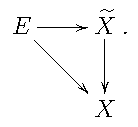
\includegraphics[width=0.1115\paperwidth]{images/L10-p081-cover.pdf}\end{figure}
$\widetilde X$存在，并且在同构意义下唯一。此时，通用覆盖$\widetilde X\to X$通过下式恢复基本群：
\begin{equation}\tag{1.1}\label{L10eq11}
\pi_1(X,x)\cong\operatorname{Aut}(\widetilde X/X).
\end{equation}
由\eqref{L10eq11}也可看出，只要通用覆盖存在，基本群的同构类型就不依赖于基点。
\originalnumber{1}
\begin{note}[L10S1O1]
拓扑空间$X$称为\textbf{半局部单连通}，是指每个点的每个邻域都含有一个子邻域，使子邻域中以该点为基点的闭路可以在$X$中缩到一点。这比每个邻域都含有单连通子邻域的条件弱。
\end{note}
\originalnumber{2}
\begin{example}\label{L10S1O2}
指数映射$\exp:\C\to\C^\times$，$a\mapsto e^{2\pi ia}$，是$\C^\times$的通用覆盖。因此，$\pi_1(\C^\times,x)\cong\operatorname{Aut}(\C/\C^\times)\cong\Z\varphi$，其中$\varphi:\C\xrightarrow{\sim}\C$，$a\mapsto a+1$。同时也可看到，指数映射不是代数映射。
\end{example}
% [Tutor Note: 原书 p81 的例 1.2 作 "is a universal covering of $\mathbb{A}^\times$"，但指数映射的靶是 $\C^\times$，下一句也写作 $\pi_1(\C^\times,x)$，故应为 $\C^\times$ 的通用覆盖；译文已按 $\C^\times$ 处理。]
在多数情形中，通用覆盖不是代数的；而且解析空间在Zariski拓扑下几乎从不是半局部单连通的。缺少代数通用覆盖时，构造基本群的代数类似物的方法，是考察有限平展覆盖\znote{有限平展覆盖是同时有限且平展的态射 $Y\to X$：有限保证几何纤维是有限集，平展则取代拓扑中「局部同构」的角色——它等价于相对微分消失（$\Omega^1_{Y/X}=0$）并配合适当的平坦性。合起来，$Y\to X$ 就是「无分支的有限覆盖」，其自同构群的逆极限给出平展基本群（见推论 1.9）。注意平展并非真正的局部同构，只是形式局部同构。[来源：nLab "etale morphism of schemes"，\url{https://ncatlab.org/nlab/show/etale+morphism+of+schemes}（Last revised 2026-07-03；2026-11-14 访问）。]}的自同构群所组成的逆系统。换言之，平展基本群都是射有限群。
\originalnumber{3}
\begin{definition}{射有限群及射有限完备化}\label{L10S1O3}\idx{射有限群}\idx{射有限完备化}
\textbf{射有限群}$\widehat G$是有限群逆系统$(G_n)$的逆极限，即$\widehat G=\varprojlim_nG_n$。若$G$为拓扑群，其\textbf{射有限完备化}为
\[G^\wedge:=\varprojlim_{\substack{U\triangleleft G\text{为开正规子群}\\{}[G:U]<\infty}}G/U.\]
\end{definition}
\sourcepage{82}
\originalnumber{4}
\begin{theorem}\label{L10S1O4}
拓扑群是射有限群，当且仅当它紧且全不连通\znoteplain{原书此处未写 Hausdorff，只假设拓扑群紧且全不连通；而射有限群按定义（有限离散群的逆极限）自动 Hausdorff 紧，若不加分离性假设，结论只在带 T0 分离公理时才成立，故通行表述通常写明 Hausdorff。阅读原书时须自行补上这一假设，正文按原书处理。（上下文推断，无外部依据）}。
\end{theorem}
一般地，给定概形$X$及几何基点$\overline x$，平展基本群$\widehat\pi_1(X,\overline x)$是射有限群，其有限连续置换表示对应于$X$上的有限平展概形。

平展态射有以下性质：
\begin{enumerate}
\item 平展性在基变换下保持。
\item 平展性在复合下保持。
\item 在交换图
\begin{figure}[H]\centering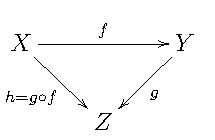
\includegraphics[width=0.1737\paperwidth]{images/L10-p082-etale.pdf}\end{figure}
中，若$g,h$平展，则$f$平展。由此可见，若$Z$连通，$h,g$有限平展，且$f$在某个几何纤维上诱导同构$X_z\cong Y_z$，则$f$为同构。
\item 有限平展态射是固有态射。
\item 平展态射局部可以表示成$\Spec B\to\Spec A$，其中
\[B\cong A[x_1,\ldots,x_n]/(f_1,\ldots,f_n),\]
且Jacobian行列式$\Delta=\det(\partial f_i/\partial x_j)$在$B$中可逆；反过来，这种局部表示给出平展态射。
\end{enumerate}
记$\mathrm{FET}/X$为$X$的有限平展覆盖范畴。对几何点$\overline x:\Spec\overline k\to X$，其中$\overline k$代数闭，有纤维函子$\mathcal F_{\overline x}:\mathrm{FET}/X\to(\mathrm{Sets})$，将$Y\to X$送到几何纤维的点集$F_{\overline x}(Y):=(Y\times_X\Spec\overline k)(\overline k)$。
\originalnumber{5}
\begin{definition}{函子的自同构}\label{L10S1O5}
设$\mathcal F:\mathcal C\to(\mathrm{Sets})$为小范畴$\mathcal C$上的函子。$\mathcal F$的一个自同构$\xi=(\xi_X)_{X\in\operatorname{Ob}(\mathcal C)}$，是
\sourcepage{83}
$\prod_{X\in\operatorname{Ob}(\mathcal C)}\operatorname{Aut}(\mathcal F(X))$中的元素，满足：对任意态射$f:X\to Y$，下图交换。
\begin{figure}[H]\centering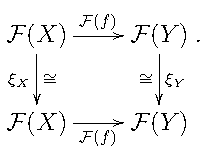
\includegraphics[width=0.1677\paperwidth]{images/L10-p083-functor.pdf}\end{figure}
因此，$\operatorname{Aut}(\mathcal F)\subset\prod_{X\in\operatorname{Ob}(\mathcal C)}\operatorname{Aut}(\mathcal F(X))$。
\end{definition}
% [Tutor Note: 原书 p83 定义 1.5 把自同构写作 $\xi=(\xi_X)_{X\in\operatorname{ob}(E)}$，其中 $E$ 应为上文的小范畴 $\mathcal C$（$\operatorname{ob}(E)$ 系排版笔误）；译文按 $\operatorname{Ob}(\mathcal C)$ 处理。]
\originalnumber{6}
\begin{definition}{平展基本群}\label{L10S1O6}
对连通概形$X$，定义其平展基本群为
\[\widehat\pi_1(X,\overline x):=\operatorname{Aut}(\mathcal F_{\overline x}),\]

\end{definition}
\originalnumber{7}
\begin{note}[L10S1O7]
对任意两个几何点$\overline x_1,\overline x_2$，有$\widehat\pi_1(X,\overline x_1)\cong\widehat\pi_1(X,\overline x_2)$。
\end{note}
注意，对$\mathrm{FET}/X$中的每个$Y\to X$，$\widehat\pi_1(X,\overline x)$作用于$F_{\overline x}(Y)$。对连通覆盖，若$|\operatorname{Aut}(Y/X)|=|F_{\overline x}(Y)|$，称$Y\to X$为\textbf{Galois覆盖}。
\originalnumber{8}
\begin{theorem}\label{L10S1O8}
若$Y$连通，则$\widehat\pi_1(X,\overline x)$在$F_{\overline x}(Y)$上传递作用。
\end{theorem}
\originalnumber{9}
\begin{corollary}\label{L10S1O9}
为连通Galois覆盖选取与$\overline x$相容的基点后，有
\[\widehat\pi_1(X,\overline x)\cong\varprojlim_{\substack{Y\to X\\\text{连通Galois覆盖}}}\operatorname{Aut}(Y/X).\]
\end{corollary}
\originalnumber{10}
\begin{example}\label{L10S1O10}
$n$次循环覆盖$\C^\times\to\C^\times$，$a\mapsto a^n$，是平展覆盖，其自同构群为$\Z/n\Z$。这些覆盖给出$\C^\times$的平展基本群$\widehat{\Z}=\varprojlim_n\Z/n\Z$。
\end{example}
\originalnumber{11}
\begin{example}\label{L10S1O11}
对任意域$k$，有$\widehat\pi_1(\Spec k,\overline k)=\Gal(k^{\mathrm{sep}}/k)$，其中$\overline k$为代数闭包，$k^{\mathrm{sep}}$为可分闭包。注意，有限扩张$L/k$可分，当且仅当$\Omega^1_{L/k}=0$。
\end{example}
\sourcepage{84}
\originalnumber{12}
\begin{example}\label{L10S1O12}
设$A$为完备离散赋值环，极大理想为$\mathfrak m$，剩余域$k\cong A/\mathfrak m$。则基变换给出范畴等价$\mathrm{FET}/\Spec A\simeq\mathrm{FET}/\Spec k$。若$\overline x:\Spec\overline k\to\Spec k$为几何点，其在$\Spec A$中的像记为$\overline y$，则
\[\widehat\pi_1(\Spec k,\overline x)\xrightarrow{\sim}\widehat\pi_1(\Spec A,\overline y).\]
\end{example}
\section{光滑层}\label{L10S2}\idx{光滑层}\idx{局部系统}
设$f:X'\to X$为连通概形之间的态射。基变换给出函子$\mathrm{FET}/X\to\mathrm{FET}/X'$。取$X'$的几何点$\overline x'$，令$\overline x=f(\overline x')$，则有射有限群的典范同态
\[f_*:\widehat\pi_1(X',\overline x')\to\widehat\pi_1(X,\overline x).\]
\originalnumber{1}
\begin{theorem}\label{L10S2O1}
设$X$为正规整Noether概形，函数域为$K$，泛点为$\eta\to X$。则典范映射
\[\Gal(K^{\mathrm{sep}}/K)\cong\widehat\pi_1(\Spec K,\overline K)\longrightarrow\widehat\pi_1(X,\overline\eta)\]
可以等同于商映射$\Gal(K^{\mathrm{sep}}/K)\to\Gal(K^{\mathrm{ur}}/K)$，其中$K^{\mathrm{ur}}$为由$X$上的有限平展覆盖所对应的扩张组成的最大处处非分歧代数扩张。因此，$\Gal(K^{\mathrm{ur}}/K)\cong\widehat\pi_1(X,\overline\eta)$。
\end{theorem}
可借助下面的正规化事实理解\eref{定理}{L10S2O1}。
\originalnumber{2}
\begin{lemma}\label{L10S2O2}
设$X$为正规整Noether概形，函数域为$K$。若$L/K$有限可分，则存在有限支配态射$Y\to X$，其中$Y$正规且整，函数域为$L$。此外，$Y\to X$平展当且仅当它非分歧\znoteplain{原书此引理既未假定正规化有限，也未限定 $X$ 为曲线：$Y$ 的存在需要 $X$ 为 Nagata 概形（正规曲线上自动成立），而「有限非分歧即平展」的等价通常也要求 $X$ 维数不超过 1 或该态射平坦。阅读时须自行补上相应假设，正文按原书处理。（上下文推断，无外部依据）}。
\end{lemma}
% [Tutor Note: 原书 p84 的引理 2.2 未提「正规化有限」与「$X$ 为正规曲线」这两项条件，译文原曾补足，现按原书回退，条件问题见上方译注。]
\eref{定理}{L10S2O1}使我们可以把$\Gal(K^{\mathrm{sep}}/K)$的处处非分歧表示看成$\widehat\pi_1(X,\Spec\overline K)$的表示。若$X$为复代数簇，还有如下比较定理。
\sourcepage{85}
\originalnumber{3}
\begin{theorem}{Grothendieck--Riemann存在定理}\label{L10S2O3}
设$X$为$\C$上局部有限型概形。把有限平展覆盖$Y\to X$送到其解析化$Y^{\mathrm{an}}\to X^{\mathrm{an}}$，给出范畴等价$\mathrm{FET}/X\simeq\mathrm{FET}/X^{\mathrm{an}}$。特别地，对复几何基点$\overline x$及相应解析点$x$，有
\[\widehat\pi_1(X,\overline x)\cong\pi_1(X^{\mathrm{an}},x)^\wedge.\]
\end{theorem}
回忆：若$X$为$\C$上的光滑射影曲线，则解析拓扑中$n$维复向量空间的局部常值层的同构类，与$\pi_1(X)$的$n$维表示的同构类一一对应。复流形解析拓扑中的局部常值层，也等价于带有全纯平坦联络的全纯向量丛。

代数几何中不能普遍使用解析拓扑，但存在类似物，即\textbf{平展拓扑}。概形$X$的平展拓扑是一种Grothen\-dieck拓扑。其中，“开集”为平展态射$U\to X$，覆盖为联合满射的态射族。$X$连通时，通过$\mathcal F\mapsto\mathcal F_{\overline x}$，有限平展局部常值层的范畴与$\widehat\pi_1(X,\overline x)$的有限连续作用范畴等价。

设$X$为$k$上的连通正规且几何连通概形，$\ell\ne\operatorname{char}(k)$，$E_\lambda$为$\Q_\ell$的有限扩张，$K$为$X$的函数域。
\originalnumber{4}
\begin{definition}{光滑$E_\lambda$层}\label{L10S2O4}
$X$上的\textbf{光滑$E_\lambda$层}\znote{光滑 $E_\lambda$ 层（lisse sheaf）就是 $E_\lambda$ 局部系统：它由 $\widehat\pi_1(X,\Spec\overline K)$ 的有限维连续 $E_\lambda$ 表示给出，秩即纤维 $V_{\mathcal F}$ 的维数。它与可构造层的关系是：光滑层在每个层上都局部常值、局部有限生成，因而是可构造层中最「局部平凡」的一类。系数取 $E_\lambda$（$\Q_\ell$ 的有限扩张）而非 $\Q_\ell$，是因为 $\ell$ 进表示的本征值一般只落在有限扩张中，取 $E_\lambda$ 后迹等不变量才落在 $E_\lambda$ 内。[来源：nLab "constructible sheaf"，\url{https://ncatlab.org/nlab/show/constructible+sheaf}（Last revised 2025-10-31；2026-11-14 访问；该条目较短，另见本讲参考文献 Milne《Lectures on étale cohomology》）。]}$\mathcal F$，亦称$E_\lambda$\textbf{局部系统}，是有限维连续$E_\lambda$表示
\[\rho_{\mathcal F}:\widehat\pi_1(X,\Spec\overline K)\to\GL(V_{\mathcal F}),\]
其中$V_{\mathcal F}$称为层的纤维，是有限维$E_\lambda$向量空间，即$V_{\mathcal F}=\mathcal F_{\Spec\overline K}$。$\mathcal F$的秩为$\operatorname{rk}(\mathcal F)=\dim_{E_\lambda}V_{\mathcal F}$。
\end{definition}
\sourcepage{86}
\section{单值表示}\label{L10S3}\idx{单值表示}\idx{外单值表示}
本节介绍通过平展基本群实现的一类Galois表示。

先看拓扑基本群上的单值作用。设$f:E\to X$为纤维化，固定基点$x\in X$及其上方的点$y\in E$。记$F_x$为$x$处的纤维，则$F_x\xrightarrow{\iota}E\xrightarrow f X$诱导同伦群长正合列
\[\begin{aligned}
\cdots\to\pi_1(F_x,y)\xrightarrow{\iota_*}\pi_1(E,y)\xrightarrow{f_*}\pi_1(X,x)\xrightarrow{\partial_y}\pi_0(F_x,y)\\
\xrightarrow{\iota_*}\pi_0(E,y)\xrightarrow{f_*}\pi_0(X,x)\to1.
\end{aligned}\]
假定$F_x$道路连通，并进一步假定$\pi_2(X,x)=0$，或者$\pi_1(F_x,y)$的中心平凡；则得到基本群的短正合列
\begin{equation}\tag{3.1}\label{L10eq31}
1\to\pi_1(F_x,y)\xrightarrow{\iota_*}\pi_1(E,y)\xrightarrow{f_*}\pi_1(X,x)\to1.
\end{equation}
对于$\sigma\in\pi_1(X,x)$，选择提升$\widetilde\sigma\in\pi_1(E,y)$，定义其对$\pi_1(F_x,y)$的外作用：
\[\rho(\sigma)(\gamma):=\widetilde\sigma\gamma\widetilde\sigma^{-1},\qquad\gamma\in\pi_1(F_x,y).\]
由于该元素属于\eqref{L10eq31}中$f_*$的核，它仍在$\pi_1(F_x,y)$中。
% [Tutor Note: 原书 p86 此处作 "since it is in the kernel of map $f_*$ in (??)"，交叉引用编号失效；按上下文应为 (3.1)，译文已按 \eqref{L10eq31} 处理。]$\rho(\sigma)$在
\[\operatorname{Out}(\pi_1(F_x,y)):=\operatorname{Aut}(\pi_1(F_x,y))/\operatorname{Inn}(\pi_1(F_x,y))\]
中的像不依赖于提升，仍记为$\rho(\sigma)$。称$\rho:\pi_1(X,x)\to\operatorname{Out}(\pi_1(F_x,y))$为$f:E\to X$在$x$上方点$y$处的\textbf{外单值表示}\znoteplain{单值表示刻画纤维化 $f:E\to X$ 的纤维沿回路一周后的变换：取回路 $\sigma\in\pi_1(X,x)$ 的提升 $\widetilde\sigma$，共轭 $\gamma\mapsto\widetilde\sigma\gamma\widetilde\sigma^{-1}$ 给出 $\pi_1(F_x,y)$ 的自同构；不同提升只差 $\pi_1(F_x,y)$ 的内自同构，故它只在 $\operatorname{Out}(\pi_1(F_x,y))$ 中有确定像，「外单值表示」之名由此而来。当存在截面 $s$（例如点 $x$ 有 $k$ 有理点）时可取 $y=s(x)$，此时外作用提升为真正的同态 $\rho_s$。「外」字提醒读者：这一作用一般不提升为 $\pi_1(X,x)\to\operatorname{Aut}(\pi_1(F_x,y))$ 的同态，只有取定截面后才得到真正的同态。（上下文推断，无外部依据）}。
% [Tutor Note: 原书 p86 定义 $\operatorname{Out}$ 时分母写作 $\pi_1(F_x,y)$（"$\operatorname{Aut}(\pi_1(F_x,y))/\pi_1(F_x,y)$"），按定义应为内自同构群 $\operatorname{Inn}(\pi_1(F_x,y))$；译文已按 $\operatorname{Inn}$ 处理。]

若选择截面$s:X\to E$，并取$y=s(x)$，则共轭作用给出典范同态$\rho_s:\pi_1(X,x)\to\operatorname{Aut}(\pi_1(F_x,y))$。当纤维基本群无中心时，有下列交换图。
\begin{figure}[H]\begin{equation}\tag{3.2}\label{L10eq32}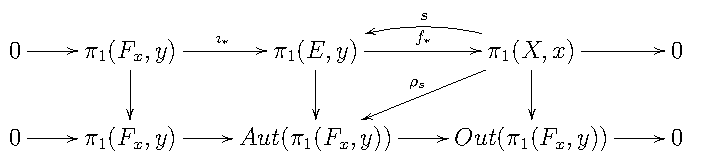
\includegraphics[width=0.5667\paperwidth]{images/L10-p086-monodromy.pdf}\end{equation}\end{figure}
平展同伦正合列也有对应的版本，即下面两个定理。
\originalnumber{1}
\begin{theorem}\label{L10S3O1}
设$f:X\to S$为平坦、固有且有限表现的概形态射，几何纤维连通且约化。假定$S$
\sourcepage{87}
连通，$\overline s:\Spec\Omega\to S$为几何点，$\overline x:\Spec\Omega\to X$为其上方的几何点。则有平展基本群正合列
\[\widehat\pi_1(X_{\overline s},\overline x)\to\widehat\pi_1(X,\overline x)\to\widehat\pi_1(S,\overline s)\to1.\]
\end{theorem}
\originalnumber{2}
\begin{theorem}\label{L10S3O2}
设$X$为域$k$上的拟紧拟分离概形，并假定$X$几何连通，即$X_{\overline k}$连通。取几何点$\overline x\in X_{\overline k}$，则存在短正合列
\[1\to\widehat\pi_1(X_{\overline k},\overline x)\to\widehat\pi_1(X,\overline x)\to\Gal(k^{\mathrm{sep}}/k)\to1.\]
\end{theorem}
沿用\eref{定理}{L10S3O2}的记号。短正合列首项$\widehat\pi_1(X_{\overline k},\overline x)$称为$X$的\textbf{几何基本群}；中间项$\widehat\pi_1(X,\overline x)$有时称为$X$的\textbf{算术基本群}。$X$的任意$k$有理点$y$给出截面$\Spec k\to X$，从而诱导截面$s_y$及同态$\rho_y$。在几何基本群无中心时，有下列交换图。
\idx{几何基本群}\idx{算术基本群}
% [Tutor Note: 原书 p87 此处作 "the first term $\widehat\pi_1(X_F,x)$"，但定理 1.2 的首项是 $\widehat\pi_1(X_{\overline k},\overline x)$，故应为 $X_{\overline k}$（$X_F$ 系笔误）；译文已作 $X_{\overline k}$。]
\begin{figure}[H]\begin{equation}\tag{3.3}\label{L10eq33}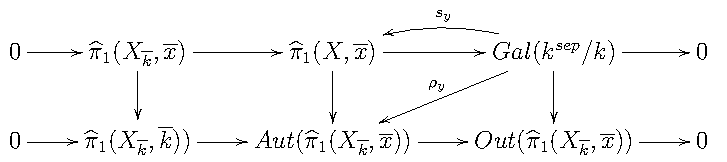
\includegraphics[width=0.5859\paperwidth]{images/L10-p087-arithmetic.pdf}\end{equation}\end{figure}
\originalnumber{3}
\begin{note}[L10S3O3]
设$A$为特征$p$的域$k$上的阿贝尔簇。当$n$与$p$互素时，$n_A:A_{\overline k}\to A_{\overline k}$为Galois有限平展覆盖，并且$\operatorname{Aut}(n_A)\cong\ker(n_A)\cong A(\overline k)[n]$。因此，当$p=0$时，
\[\widehat\pi_1(A_{\overline k},\overline0)\cong\prod_\ell T_\ell(A),\]
其中$T_\ell(A)$为$A$的Tate模。当$p>0$时，
\[\widehat\pi_1(A_{\overline k},\overline0)^{(p')}\cong\prod_{\ell\ne p}T_\ell(A).\]
对群$G$及素数$p$，$G^{(p')}$为$G$的素于$p$的完备化，即$G^{(p')}:=\varprojlim_NG/N$，逆极限遍历指数与$p$互素的正规子群$N\triangleleft G$。
\end{note}
\originalnumber{4}
\begin{note}[L10S3O4]
将光滑层$\rho_{\mathcal F}:\widehat\pi_1(X,\overline x)\to\GL(V_{\mathcal F})$限制到几何基本群$\widehat\pi_1(X_{\overline k},\overline x)$，得到与$\mathcal F$相应的几何光滑层。
\end{note}
\sourcepage{88}
\needspace{5\baselineskip}\section{第10讲参考文献}\label{L10S4}
\begin{references}
\refitem{L10bibM}{M} J. S. Milne, \emph{Lectures on étale cohomology}, Course notes. pp. 1-202. \url{http://www.jmilne.org/math/CourseNotes/CFC.pdf}.
\end{references}

\chapter{Langlands纲领的几何重述之二：阿代尔}\label{L11}\lecturedate{2020/03/23}\sourcepage{89}
已经找到了正规代数簇$X$上$n$维Galois表示的适当替代物：$X$上的秩$n$光滑层，亦即局部系统。以下两个基本事实说明这一替换是合理的。
\begin{enumerate}[label=(\roman*)]
\item 对函数域为$K$的正规代数簇$X$，有$\Gal(K^{\mathrm{ur}}/K)\cong\widehat\pi_1(X,\overline\eta)$，其中$K^{\mathrm{ur}}$为$K$相对于$X$处处非分歧的最大代数扩张。因此，在所有惯性子群上非分歧的Galois表示，可以看作平展基本群$\widehat\pi_1(X)$的表示。
\item 设$X$为连通代数簇，$\overline x$为几何点，$\mathcal F$为$X$上的局部常值层。映射$\mathcal F\mapsto\mathcal F_{\overline x}$给出范畴等价：一侧为茎有限的局部常值集合层（分别地，阿贝尔群层），另一侧为有限连续$\widehat\pi_1(X,\overline x)$集合（分别地，模）。
\end{enumerate}
本讲将进一步讨论光滑层，并为阿代尔寻找适当的几何解释。
\sourcepage{90}
\section{关于光滑层的进一步讨论}\label{L11S1}
上一讲介绍了光滑层，但还不够精确：光滑层是$\ell$进层，一般并不是单个局部常值层。

开头的事实(ii)说明，茎有限的局部常值集合层由平展基本群在几何点处茎上的作用确定。然而，若要把特征0域，例如$\Q$上的向量空间$V$实现为$\widehat\pi_1(X,\overline x)$的表示，就不能仅仅取茎为$V$的离散局部常值层。问题在于需要映射$\widehat\pi_1(X)\to\GL_n(\Q)$连续。$\widehat\pi_1(X)$带有Krull拓扑，开子群都有有限指数。若$\GL_n(\Q)$带有离散拓扑，则连续表示只能具有有限像。
% [Tutor Note: 原书 p90 作 "If we take discrete topology on $\GL_n(\Q)$, then the only continuous map $\widehat\pi_1(X)\to\GL_n(\Q)$ is zero"；但开子群的像必为有限指数，故连续同态的像只能是有限群（可以为零，也可以是有限群），译文已作「连续表示只能具有有限像」。]解决方法是用带$\ell$进拓扑的$\Q_\ell$替代$\Q$，从而把表示构造为某个逆系统的逆极限。因此，这里的局部系统是相容的局部常值层逆系统。为简单起见，只考虑$\Q_\ell$光滑层。

一个\textbf{$\ell$进层}是层的系统$(\mathcal F_n,f_{n+1}:\mathcal F_{n+1}\to\mathcal F_n)_{n\geq1}$，满足：
\begin{enumerate}
\item 对每个$n$，$\mathcal F_n$是$\Z/\ell^n\Z$模的可构造层，即存在有限个局部闭可构造子集组成的分层，使它在每个分层上局部常值且茎为有限生成模；
\item 对每个$n$，$f_{n+1}$诱导同构$\mathcal F_{n+1}/\ell^n\mathcal F_{n+1}\xrightarrow{\sim}\mathcal F_n$。
\end{enumerate}
若所有$\mathcal F_n$均为局部常值层，则这一$\ell$进层称为\textbf{光滑层}。
\originalnumber{1}
\begin{note}[L11S1O1]
有时术语略作混用，称光滑层为“局部常值$\ell$进层”；但一般不能通过一个平展覆盖同时将整个逆系统平凡化。
\end{note}
\originalnumber{2}
\begin{example}\label{L11S1O2}\idx{Tate层}\idx{Tate扭转}\idx{分圆特征标}
设$k$为域，$\mu_n$为$n$次单位根的有限群层。$\Spec k$上的Tate层\znote{Tate层 $\Z_\ell(r)$ 是 $\ell$ 进意义下的 $r$ 次扭转：它把单位根层 $\mu_{\ell^n}^{\otimes r}$ 按 $\ell$ 的幂排成逆系统，对应的连续表示正是分圆特征标的 $r$ 次幂。它在几何中扮演「上同调平移」的角色，许多簇的上同调群之间的扭转关系都用这一记号表达；不同文献的符号约定可能整体相差一个符号（$r$ 与 $-r$ 互换）。[来源：nLab "Tate twist"，\url{https://ncatlab.org/nlab/show/Tate+twist}（Last revised 2025-08-10；2026-11-14 访问）。]}
\[\Z_\ell(r):=(\mu_{\ell^n}^{\otimes r},\ f_{n+1}:\mu_{\ell^{n+1}}^{\otimes r}\to\mu_{\ell^n}^{\otimes r})_{n\geq1}\]
是光滑的，其中$\ell\ne\operatorname{char}(k)$。取相容本原单位根$\zeta_{\ell^{n+1},j}^\ell=\zeta_{\ell^n,j}$，则过渡映射为
\[f_{n+1}:\bigotimes_{j=1}^r\zeta_{\ell^{n+1},j}^{k_j}\longmapsto\bigotimes_{j=1}^r\zeta_{\ell^n,j}^{k_j}.\]
\sourcepage{91}
注意，本原单位根$\zeta_{\ell^n,j}$（$1\leq j\leq r$）给出$r$个同构$\mu_{\ell^n}\cong\Z/\ell^n\Z$，并且$\mu_{\ell^{n+1}}/\ell^n\mu_{\ell^{n+1}}\cong\mu_{\ell^n}$。

Tate层$\Z_\ell(r)$对应于连续表示
\[\Gal(k^{\mathrm{sep}}/k)\longrightarrow\Gal(k(\mu_{\ell^\infty})/k)\hookrightarrow\Z_\ell^\times\longrightarrow\operatorname{Aut}_{\Z_\ell}(\Z_\ell(r)_{\overline x}),\]
其中最后的箭头为取$r$次幂。有
\[\begin{aligned}
\operatorname{Aut}_{\Z_\ell}(\Z_\ell(r)_{\overline x})
&=\{(\xi_n)\mid\xi_n\in\operatorname{Aut}(\mu_{\ell^n}^{\otimes r}),\ f_{n+1}\xi_{n+1}=\xi_nf_{n+1}\}\\
&\cong\Z_\ell^\times.
\end{aligned}\]
因此，$\Z_\ell(r)$对应于分圆特征标的$r$次幂。显式地，若$\sigma(\zeta_{\ell^n,j})=\zeta_{\ell^n,j}^{m(n)}$，则$\chi_\ell(\sigma)=\varprojlim_nm(n)\in\Z_\ell^\times$，而$\sigma$在张量幂上的作用为
\[\chi_\ell(\sigma)^r\in\GL_1(\Z_\ell).\]
% [Tutor Note: 原书 p91 把 $\operatorname{Aut}_{\Z_\ell}(\Z_\ell(r)_{\overline x})$ 写成 $(\Z_\ell^\times)^{\otimes r}$ 型逆极限，并把 $\sigma$ 的作用写成 $Diag(\varprojlim m_1(n),\dots,\varprojlim m_r(n))\in(\Z_\ell^\times)^{\otimes r}\subset\GL_r(\Z_\ell)$；因 $\Z_\ell(r)$ 是秩 1 光滑层，自同构群应为 $\Z_\ell^\times$，作用为分圆特征标的 $r$ 次幂 $\chi_\ell(\sigma)^r\in\GL_1(\Z_\ell)$，译文已按此处理。同页原书还作 $\Gal(k(\zeta_{\ell^n})/k)\cong\Z_\ell^\times$，译文改为 $\Gal(k(\mu_{\ell^\infty})/k)\hookrightarrow\Z_\ell^\times$。]
\end{example}
有限自由$\Z_\ell$模的光滑层实际上对应于连续表示$\widehat\pi_1(X)\to\GL_r(\Z_\ell)$。形式地将其系数与$\Q_\ell$张量，就得到$\Q_\ell$光滑层。

再介绍光滑层的平展上同调。上同调一般不与层的逆极限交换。在上同调有限的情形，对$X$上的光滑层$\mathcal F=(\mathcal F_n)$，定义
\[H^r_{\mathrm{ét}}(X,\mathcal F):=\varprojlim_nH^r_{\mathrm{ét}}(X,\mathcal F_n).\]
也可以将其与$\Q_\ell$形式张量，得到$\Q_\ell$向量空间；有时仍将这一向量空间记为$H^r_{\mathrm{ét}}(X,\mathcal F)$。

平展拓扑比Zariski拓扑更细，因此，即使概形在Zariski拓扑中不可约，其有限系数局部常值层仍可具有非平凡平展上同调。
\originalnumber{3}
\begin{theorem}\label{L11S1O3}
若$X$为不可约拓扑空间，则对任意常值阿贝尔群层$\Lambda$及所有$r>0$，都有$H^r(X,\Lambda)=0$。
\end{theorem}
\begin{proof}因为$\Lambda$是松弛层。\end{proof}
在平展拓扑中，非平凡局部常值层并不具有上述松弛性质。可以取两个平展覆盖$Y_j\to X$的无交并
\sourcepage{92}
$Y_1\sqcup Y_2$，它仍为平展覆盖，但非平凡常值层的限制映射$\Lambda(X)\to\Lambda(Y_1\sqcup Y_2)=\Lambda(Y_1)\times\Lambda(Y_2)$只有对角像，不能满射。下面两个例子有助于理解平展拓扑相对于Zariski拓扑的优势。
\originalnumber{4}
\begin{example}\label{L11S1O4}\idx{Kummer正合列}
设$X$为$k$上的代数簇，$\OO_X^\times$为处处非零正则函数组成的层。取与$\operatorname{char}(k)$互素的正整数$n$。取$n$次幂诱导层态射
\begin{equation}\tag{1.1}\label{L11eq11}
\OO_X^\times\xrightarrow{\ f\mapsto f^n\ }\OO_X^\times.
\end{equation}
这一态射在Zariski拓扑中一般不满射，在平展拓扑中却满射。为简单起见，在$X=\C^\times$的情形解释。只需证明每个点$x$处的茎映射$\OO_{X,\overline x}^\times\xrightarrow{t\mapsto t^n}\OO_{X,\overline x}^\times$满射。对$t\in\OO_{X,\overline x}^\times$，存在平展态射$U\to X$，使$t$可由$U$上的可逆正则函数代表。由$t$给出映射$U\to\C^\times$，拉回$n$次平展覆盖$\C^\times\to\C^\times$，$x\mapsto x^n$，得到Cartesian图：
\begin{figure}[H]\centering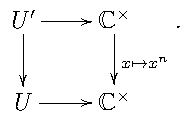
\includegraphics[width=0.1535\paperwidth]{images/L11-p092-Kummer.pdf}\end{figure}
于是$U'$仍为$x$的平展邻域，且有$\tau\in\OO_{U'}^\times$满足$\tau^n=t$。
\end{example}
\originalnumber{5}
\begin{example}\label{L11S1O5}
设$\mu_n$为$n$次单位根层，它是局部常值层。下面说明当$n>1$时，$H^1_{\mathrm{ét}}(\C^\times,\mu_n)\ne0$。利用\eqref{L11eq11}的满射得到上同调长正合列：
\begin{figure}[H]\centering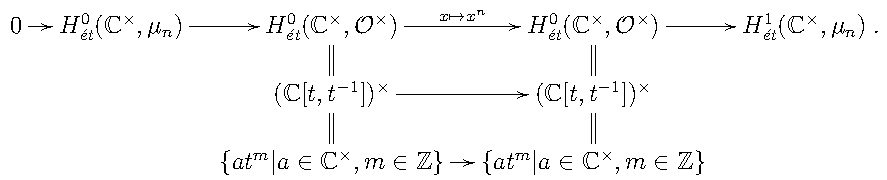
\includegraphics[width=0.7152\paperwidth]{images/L11-p092-cohomology.pdf}\end{figure}
映射$(\C[t,t^{-1}])^\times\to(\C[t,t^{-1}])^\times$，$at^m\mapsto a^nt^{mn}$，不满射，余核为$\Z/n\Z$，故$H^1_{\mathrm{ét}}(\C^\times,\mu_n)\ne0$。事实上，$H^1_{\mathrm{ét}}(\C^\times,\mu_n)\cong\Z/n\Z$。
\end{example}
\originalnumber{6}
\begin{theorem}{比较定理}\label{L11S1O6}
设$X$为$\C$上的非奇异代数簇。对任意有限阿贝尔群$\Gamma$及$r\geq0$，有$H^r_{\mathrm{ét}}(X,\Gamma)\cong H^r(X^{\mathrm{an}},\Gamma)$，其中$X^{\mathrm{an}}$为把$X$看作复流形所得的解析空间。
\end{theorem}
\sourcepage{93}
\section{阿代尔与向量丛}\label{L11S2}\idx{向量丛}\idx{除子}
先回顾两个代数事实。
\begin{itemize}
\item 若$\OO$为整闭整环，则$\OO=\bigcap_{\operatorname{ht}(\p)=1}\OO_{\p}$。
\item 若$\OO$为这样的整环，分式域为$F$，则序列
\[1\to\OO^\times\to F^\times\xrightarrow{\oplus_{\p}\ord_{\p}}\bigoplus_{\operatorname{ht}(\p)=1}\Z\to0\]
正合，当且仅当$\OO$为唯一分解整环，即UFD\znoteplain{原书此处只作「整闭整环」（integrally closed integral domain），未假定 Noether 性；而「$\OO$ 等于各高度 1 素理想局部化之交」与该序列正合 $\Leftrightarrow$ UFD 这两条事实，通常在 Noether 整闭整环（或 Krull 环）上陈述。阅读时须自行补上 Noether 假设，否则第一条事实（Krull 交定理）一般不成立；正文仍按原书处理。（上下文推断，无外部依据）}。
\end{itemize}
\originalnumber{1}
\begin{proposition}\label{L11S2O1}
设$X$为非奇异代数簇，则$X$上有层的正合列
\[1\to\OO_X^\times\to\mathcal F^\times\to\operatorname{Div}\to0,\]

\end{proposition}
设$X$为光滑代数曲线，$F$为其函数域。每个闭点$v\in X$给出$F$的一个离散赋值，局部环为UFD。这里用$\OO_x$表示其完备赋值环，$F_x$表示局部完备化。给定除子$D=\sum_{x\in|X|}n_x[x]$，由\eref{命题}{L11S2O1}，它在每个$x$处确定$F_x^\times$中$\OO_x^\times$的一个陪集$D_x\OO_x^\times$；当$n_x=0$时，该陪集就是$\OO_x^\times$。于是，$I_F/\prod_x\OO_x^\times$恰为$X$上的除子群。主除子对应于$F^\times$的元素，因此双商$F^\times\backslash I_F/\prod_x\OO_x^\times$是除子类群，也就是$X$上线丛同构类组成的群。

令$B=\prod_x\OO_x$为$\A_F$的最大紧加法子群，并令$K=\GL_n(B)$。一般地有以下结论。
\originalnumber{2}
\begin{theorem}\label{L11S2O2}
集合$\GL_n(F)\backslash\GL_n(\A_F)/K$与$X$上秩$n$向量丛的同构类集合之间存在双射。
\end{theorem}
\begin{proof}
可以按下述方式证明。对任意秩$n$向量丛$\mathcal V$，存在泛纤维的平凡化$T_X:\mathcal V\otimes_{\OO_X}F\xrightarrow{\sim}F^n$，并且对所有闭点$x$，存在局部平凡化$t_x:\OO_x^n\xrightarrow{\sim}\mathcal V\otimes_{\OO_X}\OO_x$。
\sourcepage{94}
于是有下图：
\begin{figure}[H]\centering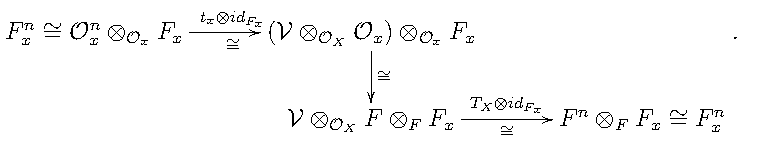
\includegraphics[width=0.6202\paperwidth]{images/L11-p094-trivialization.pdf}\end{figure}
对每个$x$，这给出元素$\mathcal V(x)\in\GL_n(F_x)$。由于$T_X$在几乎所有$x$处都诱导整平凡化，几乎所有$\mathcal V(x)$均属于$\GL_n(\OO_x)$，因此$(\mathcal V(x))_x\in\GL_n(\A_F)$。改变$T_X$或$t_x$，分别相当于在左边乘以$\GL_n(F)$中的元素，或在右边乘以$K$中的元素。
\end{proof}
现在，已为集合$\GL_n(F)\backslash\GL_n(\A_F)/K$找到几何解释，但这还不够。希望为所有秩$n$向量丛\znote{向量丛是「局部自由模」的几何版本：$X$ 上的秩 $n$ 向量丛即局部同构于 $\OO_X^{\oplus n}$ 的 $\OO_X$ 模层，等价于 $\GL_n$ 主丛（选定标架后）。在光滑曲线上，它与双商 $\GL_n(F)\backslash\GL_n(\A_F)/K$ 的同构类一一对应（定理 2.2），这是阿代尔语言与几何语言之间的桥；不做刚性化就得不到概形参数空间，只能得到模叠 $\operatorname{Bun}_n(X)$。[来源：nLab "vector bundle"，\url{https://ncatlab.org/nlab/show/vector+bundle}（Last revised 2025-10-21；2026-11-14 访问）。]}的同构类集合$\operatorname{Bun}_n(X)$赋予更多结构。可以考虑它是否由一个概形表示，但保留所有向量丛及其族的这一模问题不能直接由概形表示。要得到向量丛的参数空间，有两条途径：一是取概形形式的粗模空间，只参数化半稳定丛的$S$等价类；二是取模叠，参数化所有丛。下面采用第二条途径。
\section{模叠}\label{L11S3}\idx{模叠}\idx{代数叠}
已经看到，$\GL_n(F)\backslash\GL_n(\A_F)/K$与$\operatorname{Bun}_n(X)$中的同构类一一对应。因此，在Langlands纲领的几何表述中，用$\operatorname{Bun}_n(X)$替代这一双商。不过，$\operatorname{Bun}_n(X)$是叠，而不是概形。

叠源于模问题。对模函子而言，最理想的情形是它可以由概形表示，但这种情形并不常见。主要障碍是待参数化对象具有非平凡自同构。有时可以给对象添加额外结构，强制自同构群平凡，这称为将函子\textbf{刚性化}。例如，在固定点$x\in X$处，给每条线丛$\mathcal L$添加一个标架$\mathcal L_x\cong k$，
\sourcepage{95}
即可使次数0的线丛模问题由Jacobian概形$J(X)$表示。不过，一般模函子的刚性化可能十分复杂，并过度改变原有模问题。因此使用模叠\znote{模叠用群胚值函子记录模问题：把每个测试概形 $S$ 送去 $S$ 上的一族对象构成的群胚，从而保留对象的自同构，而不像粗模空间那样把它们压掉。代价是它只在 2 范畴意义下存在，需用 fppf 下降来陈述层性质（本节 (i)(ii) 两条）。$\operatorname{Bun}_n(X)$ 是典型例子：它不能由概形表示，但作为代数叠可由 Quot 概形的商叠局部覆盖（注 3.3）。[来源：nLab "moduli stack"，\url{https://ncatlab.org/nlab/show/moduli+stack}（Last revised 2023-04-16；2026-11-14 访问）。]}来代替概形，保留对象的全部自同构。

设$k$为基域。$k$概形$S$可看成反变函子$\underline S:(\mathrm{Sch}/k)\to(\mathrm{Sets})$，$T\mapsto\Hom(T,S)$。$S\cong S'$当且仅当$\underline S\cong\underline S'$。

一个$k$叠$\mathfrak X$首先是群胚值反变伪函子
\[\mathfrak X:(\mathrm{Sch}/k)\to(\mathrm{Gpds}),\]
其中群胚是所有态射均为同构的范畴。$(\mathrm{Gpds})$是2范畴：对两个群胚$G_1,G_2$，$\operatorname{Mor}_{\mathrm{Gpds}}(G_1,G_2)$本身也是范畴。对$S\xrightarrow f S'\xrightarrow g S''$，有三个群胚$\mathfrak X(S)$、$\mathfrak X(S')$、$\mathfrak X(S'')$，而下图仅在2范畴意义下交换：
\begin{figure}[H]\centering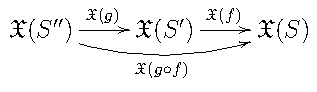
\includegraphics[width=0.2556\paperwidth]{images/L11-p095-pseudofunctor.pdf}\end{figure}
也就是说，有典范的函子同构$\alpha_{f,g}:\mathfrak X(g\circ f)\xrightarrow{\sim}\mathfrak X(f)\circ\mathfrak X(g)$。这些同构满足余循环条件：对可复合的$f,g,h$，
\[(\mathfrak X(f)\alpha_{g,h})\circ\alpha_{f,h\circ g}=(\alpha_{f,g}\mathfrak X(h))\circ\alpha_{g\circ f,h},\]
两边都是从$\mathfrak X(h\circ g\circ f)$到$\mathfrak X(f)\mathfrak X(g)\mathfrak X(h)$的自然同构。这样的函子也称为伪函子。
% [Tutor Note: 原书 p95 称这类函子为 "lax functors"，但此处要求比较同构 $\alpha_{f,g}$ 可逆、且只在 2 范畴意义下交换，按通行术语应称伪函子（pseudofunctor）；译文已作「伪函子」。]要成为$k$叠，还须满足以下两个条件。
\begin{enumerate}[label=(\roman*)]
\item 对每个$k$概形$S$及$x,y\in\operatorname{Ob}(\mathfrak X(S))$，函子
\[\begin{aligned}
\underline{\operatorname{Isom}}(x,y):\mathrm{Sch}/S&\to\mathrm{Sets},\\
(T\xrightarrow f S)&\longmapsto\Hom_{\mathfrak X(T)}(\mathfrak X(f)(x),\mathfrak X(f)(y))
\end{aligned}\]
\idx{fppf}在fppf拓扑中为层。即对任意忠实平坦且有限表现的覆盖族$\{U_i\to U\}$，有等化子序列
\[\underline{\operatorname{Isom}}(x,y)(U)\to\prod_i\underline{\operatorname{Isom}}(x,y)(U_i)\rightrightarrows\prod_{i,j}\underline{\operatorname{Isom}}(x,y)(U_{ij}),\]
其中$U_{ij}:=U_i\times_UU_j$。
\sourcepage{96}
\item 每个下降数据都有效。

对覆盖族$\{U_i\to U\}$，一个\textbf{下降数据}\znote{下降数据给「在覆盖上给出局部对象、再用同构粘起来」一个形式化：$(x_i,\varphi_{ij})$ 记录局部对象与转移同构，余循环条件保证三次交叠上相容；「有效」是说确实存在整体对象把它们粘合。叠的公理 (ii) 要求每个下降数据有效，这正是「层」条件在群胚值层面的推广，也说明了为何模叠要用 fppf 拓扑而非 Zariski 拓扑。[来源：nLab "descent"，\url{https://ncatlab.org/nlab/show/descent}（Last revised 2024-09-12；2026-11-14 访问）。]}是一族$(x_i,\varphi_{ij})$，其中$x_i\in\operatorname{Ob}(\mathfrak X(U_i))$，$\varphi_{ij}$为$\mathfrak X(U_{ij})$中的同构
\[\varphi_{ij}:x_i|_{U_{ij}}\xrightarrow{\sim}x_j|_{U_{ij}},\]
并在$U_{ijk}:=U_i\times_UU_j\times_UU_k$上满足余循环条件$\varphi_{jk}\circ\varphi_{ij}=\varphi_{ik}$。下降数据\textbf{有效}，是指存在$x\in\operatorname{Ob}(\mathfrak X(U))$及同构$\varphi_i:x|_{U_i}\xrightarrow{\sim}x_i$，使在$U_{ij}$上有$\varphi_j=\varphi_{ij}\circ\varphi_i$。
% [Tutor Note: 原书 p96 的余循环条件作 $\varphi_{ki}|_{U_{kji}}=\varphi_{kj}\circ\varphi_{ji}$，而 $U_{kji}:=U_k\times_UU_j\times_UU_i$，下标与 $U_{ijk}$ 的定义错位；译文按标准写法 $\varphi_{jk}\circ\varphi_{ij}=\varphi_{ik}$ 处理，二者在重排三元组下标后等价。]
\end{enumerate}
\idx{下降数据}
\originalnumber{1}
\begin{note}[L11S3O1]
fppf是法语“fidèlement plat et de présentation finie”的缩写，意为“忠实平坦且有限表现”。有时还会见到fpqc，它来自“fidèlement plat et quasi-compact”，意为“忠实平坦且拟紧”。
\end{note}
对任意$k$概形$S$及$\kappa\in\mathfrak X(S)$，并对$k$概形$U$上的对象$\eta\in\mathfrak X(U)$，定义$U$叠$U_\eta(\kappa)$如下：
\[\begin{aligned}
U_\eta(\kappa):\mathrm{Sch}/U&\longrightarrow\mathrm{Gpds},\\
(T\xrightarrow f U)&\longmapsto\{(\xi,\alpha)\mid\xi\in\Hom(T,S),\ \alpha:\mathfrak X(\xi)(\kappa)\xrightarrow{\sim}\mathfrak X(f)(\eta)\}.
\end{aligned}\]
其纤维化范畴中的态射$(\xi,\alpha)$到$(\xi',\alpha')$由$U$上的映射$h:T\to T'$给出，满足$\xi=\xi'\circ h$，且在相容的拉回同构下$\alpha=h^*\alpha'$。
% [Tutor Note: 原书 p96 定义 $U_\eta(\kappa)$ 时写 $h\in\Hom(T,T)$，但条件 $\xi=\xi'\circ h$（$\xi:T\to S$，$\xi':T'\to S$）要求 $h:T\to T'$，应为 $\Hom(T,T')$；译文按 $T\to T'$ 处理。]可把$\kappa$看成映射$\underline S\to\mathfrak X$，于是有Cartesian图：
\begin{figure}[H]\centering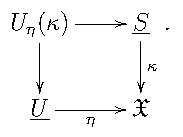
\includegraphics[width=0.1475\paperwidth]{images/L11-p096-fiber.pdf}\end{figure}
若对任意$S,\kappa,U,\eta$，$U_\eta(\kappa)$均由概形表示，并且存在$k$概形$P$及$p\in\mathfrak X(P)$，使每个基变换$U_\eta(p)\to U$均为光滑满射，则称$\mathfrak X$为代数叠。
\originalnumber{2}
\begin{theorem}\label{L11S3O2}
设$X$为连通完备光滑曲线，则$\operatorname{Bun}_n(X)$是代数叠。
\end{theorem}
\sourcepage{97}
\originalnumber{3}
\begin{note}[L11S3O3]
叠$\operatorname{Bun}_n(X)$可由参数化局部自由商$\OO_X(m)^N\twoheadrightarrow\mathcal E$的Quot概形$Q_{m,N}:=\operatorname{Quot}(\OO_X(m)^N)^{\mathrm{lf}}$中的适当开子概形覆盖。不过，不能用有限多个这样的$Q_{m,N}$覆盖全部$\operatorname{Bun}_n(X)$，因此它只是局部有限型。局部选取适当的Quot开集后，$\operatorname{Bun}_n(X)$同构于商叠$[Q_{m,N}/\GL_N]$。商叠$[Z/H]$的维数定义为$\dim Z-\dim H$。写作$\operatorname{Bun}_n(X)=\coprod_d\operatorname{Bun}_n^d(X)$，其中$\operatorname{Bun}_n^d(X)$参数化秩$n$、次数$d$的向量丛。每个这样的叠都是有限维的，尽管$n\geq2$时一般并非有限型。

若$\dim X=M\geq2$，则当$n>1$时，参数化秩$n$、Chern类$(c_1,\ldots,c_M)$向量丛的叠$\operatorname{Bun}_{n,c_1,\ldots,c_M}(X)$一般为无限维。
\end{note}
\needspace{5\baselineskip}\section{第11讲参考文献}\label{L11S4}
\needspace{4\baselineskip}\textbf{关于平展上同调。}
\begin{references}
\refitem{L11bibM}{M} J. S. Milne, \emph{Lectures on étale cohomology}, Course notes. pp. 1-202. \url{http://www.jmilne.org/math/CourseNotes/CFC.pdf}.
\end{references}
\needspace{4\baselineskip}\textbf{关于叠。}
\begin{references}
\refitem{L11bibS}{S} Ch. Sorger, \emph{Lectures on moduli of principal G-bundles over algebraic curves}, in \emph{School on algebraic geometry} (Trieste, 1999), ICTP Lecture Notes 1, ICTP, Trieste, pp. 1-57, available at \url{http://www.ictp.trieste.it/~pub_off/lectures}.
\end{references}

\chapter{Langlands纲领的几何重述之三：Hecke代数}\label{L12}\lecturedate{2020/03/25}\sourcepage{98}
在此前见过的Langlands对应中，Hecke代数和Hecke特征函数都起着关键作用。在球面情形，对应按以下方式建立：
\begin{figure}[H]\centering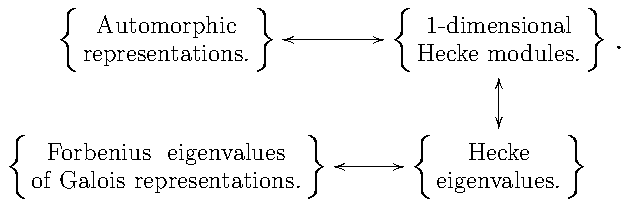
\includegraphics[width=0.5071\paperwidth]{images/L12-p098-correspondence.pdf}\end{figure}
先回顾关于Hecke代数的一个基本事实。设$F$为非阿基米德局部域，$K$为$G=\GL_n(F)$的紧开子群。与$K$相关的Hecke代数$\mathcal H_K$，是$G$上所有紧支函数$\phi$组成的向量空间，其中对任意$h_1,h_2\in K$，有$\phi(h_1gh_2)=\phi(g)$；其环结构为
\[(\phi*\psi)(g)=\int_G\phi(gx^{-1})\psi(x)\,dx,\]
其中$dx$为Haar测度。

设$\pi:G\to\GL(V)$为复向量空间$V$上的表示，$V$可能是无限维的。若对每个$0\ne v\in V$，稳定子群$G^v:=\{g\in G\mid\pi(g)v=v\}$均为开子群，则称表示\textbf{光滑}。对光滑表示$(\pi,V)$，可定义同态$\pi:\mathcal H_K\to\End(V)$：
\[\pi(\phi)v=\int_G\phi(g)\pi(g)v\,dg.\]
\sourcepage{99}
回忆：若$(\pi,V)$光滑，且对每个紧开子群$K'$，$V^{K'}$都有限维，则称它\textbf{可容许}。于是有如下定理。
\originalnumber{1}
\begin{theorem}\label{L12S0O1}
\begin{enumerate}[label=(\roman*)]
\item 若$(\pi,V)$为不可约可容许表示，且$V^K\ne0$，则$V^K$为不可约，即单的$\mathcal H_K$模。
\item 若$(\pi,V)$和$(\sigma,W)$为不可约可容许表示，且$V^K,W^K$非零并作为$\mathcal H_K$模同构，则$\pi$与$\sigma$等价。
\end{enumerate}
\end{theorem}
\begin{proof}[结论(i)的证明概要]
由于$G$全不连通且局部紧，其单位元有由紧开子群组成的邻域基。取$0\ne u\in V^K$，需要证明：对任意$v\in V^K$，存在$\phi\in\mathcal H_K$，使$\pi(\phi)u=v$。由不可约性，可写$v=\sum_ja_j\pi(g_j)u$。对每个$g=g_j$，令$K_0=gKg^{-1}\cap K$。它仍为$G$的紧开子群；由于$K$紧，$K_0$在$K$中的指数有限。于是
\[KgK=\bigsqcup_{j=1}^{N}\gamma_jgK,\]
其中$\gamma_j$为$K/K_0$的陪集代表；$KgK$具有有限测度。设$\phi_g=\operatorname{vol}(KgK)^{-1}\mathbf1_{KgK}$，其中$\mathbf1_S$为$S$的示性函数。则$\pi(\phi_g)u$是$\pi(g)u$的左$K$平均。对$v$的上述线性组合取平均，由$v\in V^K$，便有$\pi(\sum_ja_j\phi_{g_j})u=v$。
\end{proof}
\begin{proof}[结论(ii)的证明思路]
从给定的$\mathcal H_K$模同构$V^K\xrightarrow{\sim}W^K$，构造$\mathcal H$模同构$V\xrightarrow{\sim}W$，其中$\mathcal H$为$G$上局部常值紧支函数组成的卷积代数。随后这一同构也是$G$模同构：若$K_v$为包含于$G^v$的紧开子群，则对$\phi=\operatorname{vol}(K_v)^{-1}\mathbf1_{gK_v}$，有$\pi(g)v=\pi(\phi)v$。
\end{proof}
\section{几何情形中的Hecke代数}\label{L12S1}\idx{球面Hecke代数}
设$X$为完备光滑曲线，函数域为$F$。对每个素位$x\in|X|$，局部Hecke代数$\mathcal H(\GL_n(F_x),\GL_n(\OO_x))$与紧子群$\GL_n(\OO_x)$相关，亦称\textbf{球面Hecke代数}。它是交换的，并且几乎是一个多项式代数。更精确地，
\[\mathcal H(\GL_n(F_x),\GL_n(\OO_x))=\C[T_x^1,\ldots,T_x^{n-1},T_x^n,(T_x^n)^{-1}].\]
\sourcepage{100}
其中，$T_x^i$是对角矩阵
\[g_i=\operatorname{diag}(\underbrace{\omega_x,\ldots,\omega_x}_{i\text{次}},1,\ldots,1)\]
的$\GL_n(\OO_x)$双陪集的示性函数；$\omega_x$为$\OO_x$的素元，即$\ord_{\p_x}(\omega_x)=1$。换言之，$T_x^i=\mathbf1_{\GL_n(\OO_x)g_i\GL_n(\OO_x)}$。

还定义整体Hecke代数
\[\mathcal H(\GL_n(\A_F),K):=\bigotimes_{x\in|X|}'\mathcal H(\GL_n(F_x),\GL_n(\OO_x)),\]
其中照例$K=\prod_{x\in|X|}\GL_n(\OO_x)$是$\GL_n(\A_F)$的最大紧子群。它作用于$\mathcal A_0(G)^K$，即双商
\[\GL_n(F)\backslash\GL_n(\A_F)/K\]
上的尖点自守函数空间。

希望以几何语言解释Hecke算子。回忆，作为集合，$\GL_n(F)\backslash\GL_n(\A_F)/K\cong\operatorname{Bun}_n(X)$的同构类集合。因此，要在$\operatorname{Bun}_n(X)$上描述Hecke代数作用。先从集合论解释。记$\mathcal H_x^i$为数据$(\mathcal M,\mathcal M',\beta)$的同构类集合，其中$\mathcal M,\mathcal M'$为$X$上的秩$n$向量丛，$\beta:\mathcal M\hookrightarrow\mathcal M'$为嵌入，商$\mathcal M'/\mathcal M$支于$x$，被$x$的极大理想消去，且长度为$i$。记$k_x$为$x$的剩余域，则有
\begin{equation}\tag{1.1}\label{L12eq11}
\begin{aligned}
0\to\ker(\beta\otimes k_x)\to\mathcal M\otimes k_x\xrightarrow{\beta\otimes k_x}\mathcal M'\otimes k_x\\
\longrightarrow(\mathcal M'/\mathcal M)\otimes k_x\to0.
\end{aligned}
\end{equation}
其中$\ker(\beta\otimes k_x)\cong\operatorname{Tor}^{\OO_{X,x}}_1(\mathcal M'/\mathcal M,k_x)$，且$\beta\otimes k_x$的核与余核都非典范地同构于$k_x^i$。

从$\mathcal H_x^i$到$\operatorname{Bun}_n(X)$有两个映射$h^\leftarrow,h^\rightarrow$\znote{Hecke对应是向量丛模叠之间的一类对应：对每个 $i$ 与 $x\in X$，把「$\mathcal M\hookrightarrow\mathcal M'$ 且商 $\mathcal M'/\mathcal M$ 支于 $x$、长度为 $i$」的数据汇成叠 $\mathcal H_x^i$，即得对应 $\operatorname{Bun}_n(X)\xleftarrow{h^\leftarrow}\mathcal H_x^i\xrightarrow{h^\rightarrow}\operatorname{Bun}_n(X)$，其纤维是Grassmann簇。由它给出的积分变换 $(h^\rightarrow)_*(h^\leftarrow)^*$ 称为Hecke变换，在函数层面就是Hecke算子。要点是：Hecke算子并非两个函子的复合，而是「先拉回、再沿对应纤维积分」的对应运算。[来源：nLab "Hecke correspondence"，\url{https://ncatlab.org/nlab/show/Hecke+correspondence}（Last revised 2026-09-07；2026-11-14 访问）。]}，定义如下：
\begin{figure}[H]\centering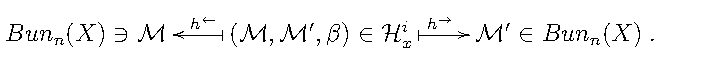
\includegraphics[width=0.5687\paperwidth]{images/L12-p100-Hecke.pdf}\end{figure}
$h^\leftarrow$的纤维典范地等同于Grassmann簇$\operatorname{Gr}(\mathcal M\otimes k_x,i)$的$k_x$点集；$h^\rightarrow$的纤维则等同于$\operatorname{Gr}(\mathcal M'\otimes k_x,n-i)$的$k_x$点集。记$\operatorname{Funct}(\operatorname{Bun}_n(X))$为其同构类上的函数空间，则有算子$(h^\rightarrow)_*(h^\leftarrow)^*$；下标$*$表示沿纤维积分，上标$*$表示拉回。
\sourcepage{101}
\originalnumber{1}
\begin{proposition}\label{L12S1O1}
算子$(h^\rightarrow)_*(h^\leftarrow)^*$等于局部Hecke代数$\mathcal H(\GL_n(F_x),\GL_n(\OO_x))$中的$T_x^i$。
\end{proposition}
把各个$\mathcal H_x^i$合在一起，得到$\mathcal H^i:=\bigcup_{x\in|X|}\mathcal H_x^i$，并有以下三个映射：
\begin{figure}[H]\centering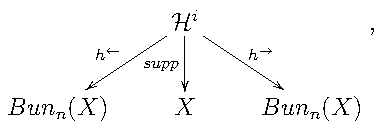
\includegraphics[width=0.3091\paperwidth]{images/L12-p101-support.pdf}\end{figure}
$\operatorname{supp}$在$x\in X$处的纤维为$\mathcal H_x^i$。

也可以用几何语言表达尖点性。取分拆$n=n_1+n_2$，考虑下列短正合列的同构类集合$\operatorname{Flag}_{n_1,n_2}^n$：
\[0\to\mathcal M_1\to\mathcal M\to\mathcal M_2\to0,\]
其中$\mathcal M_1,\mathcal M_2$分别为秩$n_1,n_2$的向量丛。有
\begin{figure}[H]\centering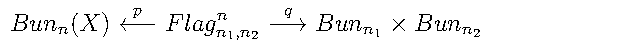
\includegraphics[width=0.5141\paperwidth]{images/L12-p101-flag.pdf}\end{figure}
这两个映射分别将短正合列送到$\mathcal M$和$(\mathcal M_1,\mathcal M_2)$。于是有
\[q_*p^*:\operatorname{Funct}(\operatorname{Bun}_n(X))\to\operatorname{Funct}(\operatorname{Bun}_{n_1}(X)\times\operatorname{Bun}_{n_2}(X)).\]
函数$f$具有尖点性，当且仅当对所有满足$n_1+n_2=n$的正整数$n_1,n_2$，都有$q_*p^*(f)=0$。然而，几何情形中用来解释自守表示的实际对象，是反常层，而不是函数。
\section{从函数到层}\label{L12S2}\idx{层与函数的对应}\idx{反常层}
先设$V$为$\F_q$上的代数簇，$Y=V(\F_q)$为其$\F_q$点集，$\mathcal F$为$V$上的$\ell$进$\overline{\Q}_\ell$层。对$x\in Y$上方的几何点$\overline x$，
\sourcepage{102}
茎$\mathcal F_{\overline x}$为$\overline{\Q}_\ell$向量空间，并带有$\Gal(\overline{k_x}/k_x)=\Gal(\overline{\F}_q/\F_q)$的自然作用，给出同态$\rho_x:\Gal(\overline{k_x}/k_x)\to\GL(\mathcal F_{\overline x})$。几何Frobenius元素$\mathrm{Fr}_x$拓扑生成这一Galois群。因此可在$Y$上定义函数
\begin{equation}\tag{2.1}\label{L12eq21}
f_{\mathcal F}:Y\to\overline{\Q}_\ell,\qquad f_{\mathcal F}(x)=\Tr(\rho_x(\mathrm{Fr}_x)).
\end{equation}
\originalnumber{1}
\begin{note}[L12S2O1]
一个$\ell$进$\overline{\Q}_\ell$层$\mathcal F$可以在某个$\Q_\ell$的有限扩张$E$上定义：取其整数环$\OO_E$上的$\ell$进层$\mathcal F_{\OO_E}$，形式地与$\overline{\Q}_\ell$张量。相应平展上同调为
\[H^r_{\mathrm{ét}}(\mathcal F)=H^r_{\mathrm{ét}}(\mathcal F_{\OO_E})\otimes_{\OO_E}\overline{\Q}_\ell,\]
因而是$\overline{\Q}_\ell$向量空间。
\end{note}
% [Tutor Note: 原书 p102 的 Remark 2.1 把 $\overline{\Q}_\ell$ 层说成「$\Z_\ell$ 层形式张量 $\Q_\ell$」，上同调也写作 $\otimes_{\Z_\ell}\Q_\ell$；译文按通行定义改为取某个 $\Q_\ell$ 的有限扩张 $E$，用其整数环 $\OO_E$ 上的层与 $\overline{\Q}_\ell$ 张量。]
\eqref{L12eq21}中的函数定义可以推广到$\ell$进层复形。设$\mathcal K^\bullet$为这样的复形，则$\Gal(\overline{k_x}/k_x)$作用于上同调层$\mathcal H^i(\mathcal K^\bullet)$在$\overline x$处的茎。定义
\begin{equation}\tag{2.2}\label{L12eq22}
f_{\mathcal K^\bullet}(x):=\sum_i(-1)^i\Tr(\mathrm{Fr}_x\mid\mathcal H^i(\mathcal K^\bullet)_{\overline x}).
\end{equation}
\eqref{L12eq22}提示，可以使用有界可构造导出范畴$D^b_c(V)$中的对象，而不只使用层。然而，$D^b_c(V)$并非阿贝尔范畴。适当的选择是反常层范畴：反常层并非通常意义的层，而是满足其茎与余茎上同调非零次数限制的$\ell$进层复形。

已经说明了$\F_q$上的代数簇中函数与层的关系。对$\C$上的代数簇，反常层的概念也完全有意义。此外，还可以进一步将反常层重述为$\mathcal D$模。后续各讲将详细介绍反常层和$\mathcal D$模。

现在的问题是：如何在$\operatorname{Bun}_n(X)$上定义层，乃至导出范畴$D^b_c(\operatorname{Bun}_n(X))$？$n=1$时，次数0线丛的刚性化模问题由代数概形$\operatorname{Jac}(X)$表示。一般地，$\operatorname{Bun}_n(X)$只是代数叠。

要在叠上定义层，可以从概形转向函子。如上一讲所述，每个$k$概形$S$都关联反变函子$\underline S:(\mathrm{Sch}/k)\to\mathrm{Sets}$，$T\mapsto\Hom(T,S)$。
\sourcepage{103}
由Yoneda引理，概形由其函子完全确定。叠$\mathfrak X$也是函子，且$\Hom(\underline S,\mathfrak X)$为范畴$\mathfrak X(S)$。在$\mathfrak X$上定义$\ell$进层，是给每个对象$\eta\in\mathfrak X(S)$赋予$S$上的$\ell$进层，并给每个箭头赋予层之间的同构，同时要求这些数据与基变换相容。于是，$D^b_c(\mathfrak X)$也有意义。特别地，$\mathfrak X$的$\F_q$点实际构成范畴$\mathfrak X(\Spec\F_q)$；每个$\mathcal F\in D^b_c(\mathfrak X)$都给出其对象同构类上的函数$f_{\mathcal F}$。

现在把$\operatorname{Bun}_n(X)$看成代数叠。$\mathcal H_x^i$、$\mathcal H^i$也具有叠结构。因此，$h^\leftarrow,h^\rightarrow$是叠之间的态射，其纤维为概形形式的Grassmann簇。它们可表示，所以可以讨论相应的拉回和推前。定义Hecke函子
\[T_x^i:D^b_c(\operatorname{Bun}_n(X))\to D^b_c(\operatorname{Bun}_n(X)),\]
由
\[\mathcal K^\bullet\longmapsto(h^\rightarrow)_*(h^\leftarrow)^*(\mathcal K^\bullet)[i(n-i)]\]
给出。上下标$*$在这里均指导出函子；方括号表示上同调平移（Tate 平移）。

还定义Hecke函子$T^i:D^b_c(\operatorname{Bun}_n(X))\to D^b_c(X\times\operatorname{Bun}_n(X))$：
\[\mathcal K^\bullet\longmapsto(\operatorname{supp}\times h^\rightarrow)_*(h^\leftarrow)^*(\mathcal K^\bullet)[i(n-i)].\]
\idx{Hecke函子}
\section{Langlands对应的几何表述}\label{L12S3}\idx{几何Langlands对应}\idx{Hecke特征层}
在几何Langlands猜想\znote{几何Langlands对应是经典Langlands对应的几何化：Galois表示一侧换成曲线 $X$ 上的局部系统，自守表示一侧换成 $\operatorname{Bun}_n(X)$ 上的反常层（Hecke特征层），并在两者之间建立函子性的对应。与经典情形给出「表示的对应」不同，几何版本预期是范畴层面的对应：平坦联络的局部系统与 $\operatorname{Bun}_n(X)$ 上的反常层（或相应范畴中的对象）应当互相对应；本讲只陈述其中单向的构造，即由局部系统造出Hecke特征层。[来源：nLab "Langlands program"，\url{https://ncatlab.org/nlab/show/Langlands+program}（Last revised 2024-03-28；2026-11-14 访问）。]}中，以曲线$X$上的$n$维局部系统替代经典理论中的Galois表示；在自守一侧，则使用叠$\operatorname{Bun}_n(X)$上的反常层，即Hecke特征层。这里的几何Langlands对应按从局部系统到Hecke特征层的单向映射表述，因为Hecke特征层是相对于局部系统定义的。

设$E=E_\sigma$为$X$上的$\overline{\Q}_\ell$局部系统，对应表示
\sourcepage{104}
$\sigma:\widehat\pi_1(X)\to\GL_n(\overline{\Q}_\ell)$。若对每个$i=1,\ldots,n$，存在同构
\[T^i(\mathcal F_\sigma)\cong\bigwedge^iE_\sigma\boxtimes\mathcal F_\sigma,\]
则称$\mathcal F_\sigma\in D^b_c(\operatorname{Bun}_n(X))$为相对于$\sigma$的\textbf{Hecke特征层}\znote{Hecke特征层是Hecke变换的本征对象：要求对每个 $i$ 都有 $T^i(\mathcal F_\sigma)\cong\bigwedge^iE_\sigma\boxtimes\mathcal F_\sigma$，即Hecke变换把 $\mathcal F_\sigma$ 送到自身的「张量倍数」，倍数由局部系统 $E_\sigma$ 的外幂丛 $\bigwedge^iE_\sigma$ 给出。这与经典理论中Hecke特征函数的地位平行：自守表示被Hecke算子作用后仍是自身的倍数，倍数即Hecke本征值；几何化之后本征值由外幂丛取代。注意 eigensheaf 是按定义相对于某个局部系统而言的，故几何Langlands对应只能是单向的映射。[来源：nLab "Hecke eigensheaf"，\url{https://ncatlab.org/nlab/show/Hecke+eigensheaf}（该条目较短且未标注 Last revised，2026-11-14 访问；另参 "Hecke correspondence"）。]}；其中$\bigwedge^i$表示第$i$次外幂。

几何Langlands对应由以下定理表述。
\originalnumber{1}
\begin{theorem}\label{L12S3O1}
设$X$为定义在$\F_q$或$\C$上的光滑完备曲线。对$X$上的每个不可约秩$n$局部系统$E$，都存在反常层$\mathcal F_\sigma\in D^b_c(\operatorname{Bun}_n(X))$，它是相对于$E$的Hecke特征层，并自动具有尖点性。此外，在每个参数化秩$n$、次数$d$向量丛的连通分量$\operatorname{Bun}_n^d(X)$上，$\mathcal F_\sigma$不可约。
\end{theorem}
换言之，这一几何表述断言存在如下单向对应：
\begin{figure}[H]\centering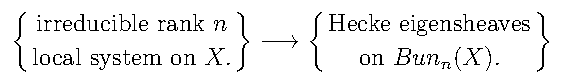
\includegraphics[width=0.4549\paperwidth]{images/L12-p104-correspondence.pdf}\end{figure}
\originalnumber{2}
\begin{note}[L12S3O2]
这里在Galois一侧只考虑处处非分歧表示，在自守一侧只考虑所有局部分量$\pi_x$均为球面表示的$\pi=\bigotimes_x'\pi_x$。而经典Langlands纲领中的Galois表示仅要求几乎处处非分歧，自守表示也仅要求几乎处处球面。在允许有限多个素位处分歧的更一般几何情形中，也有一些结果，但本课程不讨论它们。
\end{note}
\needspace{5\baselineskip}\section{第12讲参考文献}\label{L12S4}
\begin{references}
\refitem{L12bibBG}{BG} J. Bernstein and S. Gelbart, eds, \emph{An introduction to the Langlands Program}, Birkhäuser, 2004, Chapter 12 written by D. Gaitsgory.
\end{references}

\addtocontents{toc}{\protect\newpage}
\chapter{插讲：反常层}\label{L13}\lecturedate{2020/03/30}\sourcepage{105}
本讲介绍反常层的定义及若干性质。多数结论不在这里证明，读者可以在参考文献中查阅证明。

一般而言，反常层是同时满足\textbf{支撑条件}和\textbf{余支撑条件}的层复形。反常层之所以重要，一个原因是它们在Verdier对偶下具有良好的性质。我们先简要介绍Verdier对偶\znote{Verdier对偶是局部紧、有限维空间 $X$ 的导出范畴上的对合函子，形式为 $\mathbb D_X(\mathcal F^\bullet)=\mathrm R\mathcal Hom(\mathcal F^\bullet,\omega_X)$，其中 $\omega_X=\mathbb D_X(k_X)$ 称为对偶化复形。它把紧支上同调与普通上同调配对：$H^r_c(X,\mathcal F)^\vee\cong H^{-r}(X,\mathbb D_X\mathcal F)$。当 $X$ 是 $n$ 维光滑流形时 $\omega_X=k_X[n]$，上式即经典的Poincaré对偶；对奇异空间，对偶化复形承担了「定向」的角色。易错点是 $\mathbb D_X$ 作用于复形而非单个层。[来源：nLab "Verdier duality"，\url{https://ncatlab.org/nlab/show/Verdier+duality}（Last revised 2026-08-11；2026-11-14 访问；该条目内容较简，另见 Peters--Steenbrink《Mixed Hodge Structures》Ch. 13 §13.1）。]}：它将Poincaré对偶推广到局部紧、有限维的拓扑空间。Verdier对偶处理的是复形，更确切地说，是导出范畴中的对象。
\originalnumber{1}
\begin{definition}\label{L13S0O1}
设$X$为局部紧空间。其\textbf{维数}$\dim X$是使得对$X$上的任意阿贝尔群层$\mathcal F$均有$H_c^{n+1}(X,\mathcal F)=0$的最小非负整数$n$；若不存在这样的整数，则维数为$\infty$。这里$H_c^j(X,\cdot)$表示紧支上同调，即$\Gamma_c(X,\cdot)$的第$j$个右导出函子。
\end{definition}
\originalnumber{2}
\begin{note}[L13S0O2]
复维数为$n$的复空间，其上述维数为$2n$。
\end{note}
\section{Verdier对偶}\label{L13S1}\idx{Verdier对偶}\idx{紧支上同调}
设$X$为$n$维局部紧空间。对任意层$\mathcal F$，可以选取内射消解
\[\mathcal F\hookrightarrow\mathcal I^\bullet(\mathcal F).\]
$\mathcal I^\bullet$可能含有无穷多项，因此定义它的$n$次截断复形为以下含$n+1$项的复形：
\begin{equation}\tag{1.1}\label{L13eq11}
\begin{aligned}
{}_c\mathcal I^\bullet(\mathcal F)&:=\tau_{\le n}\mathcal I^\bullet(\mathcal F)\\
&=\bigl(\mathcal I^0(\mathcal F)\to\mathcal I^1(\mathcal F)\to\cdots\to\mathcal I^{n-1}(\mathcal F)\to\ker(\mathcal I^n(\mathcal F)\to\mathcal I^{n+1}(\mathcal F))\bigr).
\end{aligned}
\end{equation}
\sourcepage{106}
于是${}_c\mathcal I^\bullet(\mathcal F)$是$\mathcal F$的$\Gamma_c$-零调消解\idx{零调消解}。若$\mathcal F^\bullet$是有界层复形，同样可以为它构造有限长度的$\Gamma_c$-零调消解${}_c\mathcal I^\bullet(\mathcal F^\bullet)$。

设$k$为域。层复形$\mathcal F^\bullet$的\textbf{Verdier对偶}$\mathbb D_X(\mathcal F^\bullet)$，是由以下预层复形给出的层复形：对任意开集$U\subseteq X$，
\begin{equation}\tag{1.2}\label{L13eq12}
\mathbb D_X(\mathcal F^\bullet)(U):=\Hom_k^\bullet(C^\bullet(U),k),
\end{equation}
其中$C^\bullet(U)=\Gamma_c(U,{}_c\mathcal I^\bullet(\mathcal F^\bullet))$，且$\Hom^q(C^\bullet(U),k):=\Hom_k(C^{-q}(U),k)$。有如下结论。
\originalnumber{1}
\begin{proposition}[Verdier对偶]\label{L13S1O1}
设$X$为$n$维局部紧空间，$\mathcal F^\bullet$为有界层复形，则
\[\mathbb D_X(\mathcal F^\bullet)\cong\mathrm R\mathcal Hom(\mathcal F^\bullet,\mathbb D_X(k_X)),\]
其中$k_X$为$X$上茎为$k$的常值层。
\end{proposition}
更一般地，设$f:X\to Y$为两个局部紧空间之间的连续映射。考虑以下四个函子$f_!,f_*,f^!,f^{-1}$。
\begin{itemize}
\item $f_*$为直像函子，是左正合函子；若$Y=\mathrm{pt}$，则$f_*=\Gamma(\cdot)$。
\item $f_!$为真直像函子；若$Y=\mathrm{pt}$，则$f_!=\Gamma_c(\cdot)$。若$f$为真映射，则$f_!=f_*$。
\item $f^{-1}$为逆像函子，是正合函子。
\item $f^!$为非常逆像；若$f$为开嵌入，则$f^!=f^{-1}$。
\end{itemize}
按定义，$f^!$是$\mathrm Rf_!$在导出范畴中的右伴随（一般情形未必存在）。设$\mathcal G^\bullet$为$Y$上的有界层复形，则$f^!\mathcal G^\bullet$是$X$上的有界层复形。其开集$U$上的构造可写为
\begin{equation}\tag{1.3}\label{L13eq13}
U\longmapsto\Hom_Y^\bullet\bigl(f_!j_!{}_c\mathcal I^\bullet(k_U),\mathcal J^\bullet(\mathcal G^\bullet)\bigr),\qquad j:U\hookrightarrow X,
\end{equation}
其中$\mathcal J^\bullet(\mathcal G^\bullet)$为内射消解。
\originalnumber{2}
\begin{theorem}[Verdier对偶II]\label{L13S1O2}
设$f:X\to Y$为有限维局部紧空间之间的连续映射。对$Y$上的有界复形$\mathcal K^\bullet$和$X$上的有界复形$\mathcal L^\bullet$，有典范同构
\[\mathrm R\mathcal Hom_Y(\mathcal K^\bullet,\mathrm Rf_*\mathcal L^\bullet)\xrightarrow{\sim}\mathrm Rf_*\bigl(\mathrm R\mathcal Hom_X(f^{-1}\mathcal K^\bullet,\mathcal L^\bullet)\bigr).\]
对$X$上的有界复形$\mathcal F^\bullet$和$Y$上的有界复形$\mathcal G^\bullet$，有典范同构
\sourcepage{107}
\[\mathrm R\mathcal Hom_Y(\mathrm Rf_!\mathcal F^\bullet,\mathcal G^\bullet)\xrightarrow{\sim}\mathrm Rf_*\bigl(\mathrm R\mathcal Hom_X(\mathcal F^\bullet,f^!\mathcal G^\bullet)\bigr).\]
这些同构位于$D^b(Y;k)$，即$Y$上$k$-模层的有界导出范畴。此外有下图：
\begin{figure}[H]\centering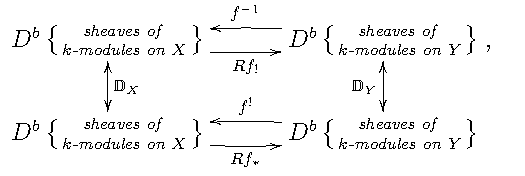
\includegraphics[width=0.4232\paperwidth]{images/L13-p107-duality.pdf}\end{figure}
它包含两个交换关系：
\[\mathrm Rf_*\circ\mathbb D_X\cong\mathbb D_Y\circ\mathrm Rf_!,\qquad \mathbb D_X\circ f^{-1}\cong f^!\circ\mathbb D_Y.\]
\end{theorem}
\originalnumber{3}
\begin{note}[L13S1O3]
域$k$可以换成具有有限同调维数的含幺交换环$R$；特别地，$R$本身具有有限长度的内射消解。例如可以取$R=\Z$。设$R\hookrightarrow\mathcal R^\bullet$为$R$的内射消解，则将\eqref{L13eq12}中的$\Hom_k^\bullet(-,k)$换成$\Hom_R^\bullet(-,\mathcal R^\bullet)$，其余构造与前面类似。
\end{note}
\section{反常层}\label{L13S2}\idx{支撑条件}\idx{余支撑条件}\idx{分层}\idx{Whitney分层}
设$k$为域，或具有有限同调维数的含幺交换环；$X$为复解析簇。代数簇$X$的一个\textbf{分层}，是将$X$分解为有限多个两两不交的部分，亦称\textbf{层}：
\[X=\coprod_{\lambda\in\Lambda}X_\lambda,\]
且满足：
\begin{enumerate}[label=(\arabic*)]
\item 每个$X_\lambda$连通、光滑，且在Zariski拓扑下局部闭；
\item 每一层的闭包都是若干层的并。
\end{enumerate}
\originalnumber{1}
\begin{definition}\label{L13S2O1}
\begin{enumerate}[label=\arabic*.]
\item 固定分层$X=\coprod_{\lambda\in\Lambda}X_\lambda$。若$X$上的$k$-模层$\mathcal F$在每层上的限制$\mathcal F|_{X_\lambda}$都是局部常值、局部有限生成的$k$-模层，则称$\mathcal F$为\textbf{$\Lambda$-可构造层}。若对某个分层$\Lambda$它是$\Lambda$-可构造层，则称它为\textbf{可构造层}。
\sourcepage{108}
\item 若层复形$\mathcal F^\bullet$的全部上同调层$\mathcal H^i(\mathcal F^\bullet)$都是可构造的，分别是$\Lambda$-可构造的，则称该复形可构造，分别为$\Lambda$-可构造。$D^b(X)$中由可构造复形、分别由$\Lambda$-可构造复形组成的满子范畴记为$D_c^b(X)$、分别记为$D_\Lambda^b(X)$。
\end{enumerate}
\end{definition}
\originalnumber{2}
\begin{note}[L13S2O2]
局部常值、局部有限生成的层也称为局部系统。注意，解析情形中的局部系统是局部常值的，而平展拓扑中的$\ell$进局部系统未必能在某个平展覆盖下平凡化。
\end{note}
\originalnumber{3}
\begin{proposition}\label{L13S2O3}
设$X,Y$为复解析簇。
\begin{enumerate}[label=(\arabic*)]
\item 导出张量积和导出$\mathcal Hom$函子都保持可构造性。
\item Verdier对偶算子$\mathbb D_X$保持可构造性。
\item 若$f:X\to Y$为态射，则$f^{-1}$和$f^!$保持可构造性。若$f$为真映射，或为复代数簇之间的态射，则$\mathrm Rf_*$和$\mathrm Rf_!$也保持可构造复形。
\end{enumerate}
\end{proposition}
设$f:X\to Y$为真映射。现在以$D_c^b(-)$代替$D^b(-)$来讨论，有如下结论。
\originalnumber{4}
\begin{theorem}\label{L13S2O4}
\begin{enumerate}[label=\arabic*.]
\item Verdier对偶算子$\mathbb D_X$是对合，即$\mathbb D_X^2\cong\mathrm{Id}$。
\item \textbf{真基变换：}对任意下列Cartesian图，其中底边映射记为$g:Y'\to Y$（顶边为$f:X\to Y$，右边为$f':X'\to X$，左边为$g':X'\to Y'$），
\begin{figure}[H]\centering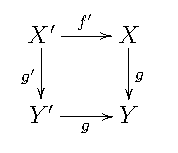
\includegraphics[width=0.1434\paperwidth]{images/L13-p108-basechange.pdf}\end{figure}
有函子同构
\[f^{-1}\circ\mathrm Rg_!\cong\mathrm Rg'_!\circ f'^{-1}.\]
\item \textbf{投影公式：}有函子同构
\[(\mathrm Rf_!(-))\otimes^{\mathrm L}(-)\cong\mathrm Rf_!\bigl((- )\otimes^{\mathrm L}f^{-1}(-)\bigr),\]
其中$\otimes^{\mathrm L}$表示导出张量积。
\sourcepage{109}
\item 有函子同构
\[\mathrm R\mathcal Hom(f^{-1}(-),f^!(-))\cong f^!\mathrm R\mathcal Hom(-,-).\]
\item \textbf{开闭三角：}设$U\hookrightarrow X$为Zariski开嵌入，$Z=X\setminus U$；令$j:U\to X$、$i:Z\to X$分别为开、闭嵌入。则在$D^b(X)$中有函子性的正合三角
\[i_!i^!\to\mathrm{Id}\to\mathrm Rj_*j^*\xrightarrow{[1]},\qquad j_!j^!\to\mathrm{Id}\to i_*i^*\xrightarrow{[1]}.\]
\end{enumerate}
\end{theorem}
\originalnumber{5}
\begin{definition}\label{L13S2O5}
固定分层$X=\coprod_{\lambda\in\Lambda}X_\lambda$，使$\mathbb D_X$保持$D_\Lambda^b(X)$，例如可以取Whitney分层。若$\Lambda$-可构造层复形$\mathcal F^\bullet$满足下列两个条件，则称它是相对于$\Lambda$的\textbf{反常层}\znote{反常层由 Beilinson--Bernstein--Deligne 在研究六函子形式时引入，perverse 一词只表明其截断位置与通常层复形相反；它并不是层，而是满足支撑条件与余支撑条件的可构造复形。两个条件把上同调挤进与分层维数匹配的窄区间：在复维数 $d$ 的层 $X_\lambda$ 上只允许 $j\le-d$ 的 $\mathcal H^j$，余支撑条件则对偶地限制 $i_x^!\mathcal F^\bullet$ 的非零范围。关键结论是 $\operatorname{Perv}(X)$ 为阿贝尔范畴，而 $D_c^b(X)$ 不是，因此反常层上可以谈论子对象、商对象与单性。[来源：nLab "perverse sheaf"，\url{https://ncatlab.org/nlab/show/perverse+sheaf}（Last revised 2026-10-16；2026-11-14 访问）。]}：
\[\begin{cases}
\mathcal H^j(\mathcal F^\bullet)_x=0,&x\in X_\lambda,\ j>-\dim_{\C}X_\lambda,\\
\mathcal H^j(i_x^!\mathcal F^\bullet)=0,&x\in X_\lambda,\ j<\dim_{\C}X_\lambda.
\end{cases}\]
这里$i_x:\{x\}\hookrightarrow X$。若$\mathcal F^\bullet$相对于某个分层$\Lambda$为反常层，就称它为反常层。$D_c^b(X)$中由$k$-模反常层组成的满子范畴记为$\operatorname{Perv}(X)$。
\end{definition}
\originalnumber{6}
\begin{note}[L13S2O6]
\textbf{Whitney分层}是满足Whitney条件的分层：设$X_\mu\subseteq\overline{X_\lambda}$，有点列$\{a_n\}\subseteq X_\mu$、$\{b_n\}\subseteq X_\lambda$，两者都趋于同一点$c\in X_\mu$。若连接$a_n,b_n$的割线以及$X_\lambda$在$b_n$处的切空间分别存在极限，则割线的极限包含于切空间的极限中。

每个复代数簇都具有Whitney分层；并且任意分层都可以细化为Whitney分层。
\end{note}
\originalnumber{7}
\begin{lemma}\label{L13S2O7}
设$k$为特征零的域，$\mathcal F^\bullet$为有界可构造$k$-模层复形。它为反常层，当且仅当满足下列两条件：
\[\begin{aligned}
\dim_{\C}\operatorname{Supp}\mathcal H^j(\mathcal F^\bullet)&\le-j&&\text{（支撑条件）},\\
\dim_{\C}\operatorname{Supp}\mathcal H^j(\mathbb D_X(\mathcal F^\bullet))&\le-j&&\text{（余支撑条件）}.
\end{aligned}\]
特别地，$\mathcal F^\bullet$为反常层，当且仅当其Verdier对偶$\mathbb D_X(\mathcal F^\bullet)$为反常层；反常性不依赖于所选的分层。
\end{lemma}
\sourcepage{110}
定义反常层的另一种方式，是把$\operatorname{Perv}(X)$看作三角范畴$D_c^b(X)$的某个截断结构的\textbf{心}。以$[n]$表示平移函子，约定$(\mathcal F^\bullet[n])^q=\mathcal F^{n+q}$。
\originalnumber{8}
\begin{definition}\label{L13S2O8}\idx{t结构}\idx{心（t结构）}
三角范畴$D$上的\textbf{截断结构}，简称\textbf{$t$结构}\znote{$t$结构是对三角范畴中「截断」的公理化：一对满子范畴 $(D^{\le0},D^{\ge0})$ 保证每个对象 $S$ 都同构意义下唯一地落入三角 $A\to S\to B\xrightarrow{[1]}$，其中 $A\in D^{\le0}$、$B\in D^{\ge1}$，于是可以定义截断函子 ${}^t\tau_{\le0}$、${}^t\tau_{\ge1}$ 与上同调函子 ${}^t\mathcal H^n$。其心 $C(D,t)=D^{\le0}\cap D^{\ge0}$ 自动是阿贝尔范畴，这是 $t$ 结构最重要的性质。阿贝尔范畴的导出范畴上由 $\mathcal H^j$ 的消失范围给出标准 $t$ 结构；本讲后文要说明 $D_c^b(X)$ 上还存在反常 $t$ 结构，其心正是 $\operatorname{Perv}(X)$。[来源：nLab "t-structure"，\url{https://ncatlab.org/nlab/show/t-structure}（Last revised 2023-04-20；2026-11-14 访问）。]}，是一对满子范畴$(D^{\le0},D^{\ge0})$，满足：
\begin{enumerate}[label=(\roman*)]
\item 令$D^{\le n}:=D^{\le0}[-n]$、$D^{\ge n}:=D^{\ge0}[-n]$，则$\Hom(D^{\le0},D^{\ge1})=0$。
\item $D^{\le-1}\subseteq D^{\le0}$且$D^{\ge1}\subseteq D^{\ge0}$。
\item 任意$S\in\operatorname{ob}(D)$都属于一个区别三角
\begin{equation}\tag{2.1}\label{L13eq21}A\to S\to B\xrightarrow{[1]},\end{equation}
其中$A\in D^{\le0}$、$B\in D^{\ge1}$。
\end{enumerate}
给定$t$结构的\textbf{心}，亦称核心，定义为$C(D,t):=D^{\le0}\cap D^{\ge0}$。
\end{definition}
\originalnumber{9}
\begin{example}\label{L13S2O9}
阿贝尔范畴$\mathcal A$的导出范畴$D(\mathcal A)$上有一个自然的$t$结构：
\[\begin{aligned}
\operatorname{ob}(D^{\le0})&:=\{\mathcal G^\bullet\in\operatorname{ob}(D(\mathcal A))\mid\mathcal H^j(\mathcal G^\bullet)=0,\ \forall j>0\},\\
\operatorname{ob}(D^{\ge0})&:=\{\mathcal G^\bullet\in\operatorname{ob}(D(\mathcal A))\mid\mathcal H^j(\mathcal G^\bullet)=0,\ \forall j<0\}.
\end{aligned}\]
该$t$结构的心等价于阿贝尔范畴$\mathcal A$。
\end{example}
由下面的\eref{引理}{L13S2O10}，\eqref{L13eq21}中的对应$S\mapsto A$、分别$S\mapsto B$给出良定义的函子，记为${}^t\tau_{\le0}$、分别记为${}^t\tau_{\ge1}$。类似地，定义
\[{}^t\tau_{\le a}:=[-a]\circ{}^t\tau_{\le0}\circ[a],\qquad {}^t\tau_{\ge b}:=[1-b]\circ{}^t\tau_{\ge1}\circ[b-1].\]
对任意$a,b\in\Z$，有典范同构${}^t\tau_{\le a}\circ{}^t\tau_{\ge b}\cong{}^t\tau_{\ge b}\circ{}^t\tau_{\le a}$。
\sourcepage{111}
\originalnumber{10}
\begin{lemma}\label{L13S2O10}
设$D$为三角范畴，考虑两个区别三角$A\to S\to B\xrightarrow{[1]}$、$A'\to S'\to B'\xrightarrow{[1]}$和$D$中的映射$g:S\to S'$。考虑下图：
\begin{figure}[H]\centering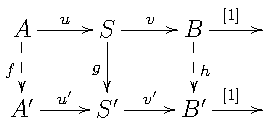
\includegraphics[width=0.2242\paperwidth]{images/L13-p111-triangles.pdf}\end{figure}
下列条件等价：
\begin{enumerate}[label=(\arabic*)]
\item 存在$f$，使第一个方块交换；
\item 存在$h$，使第二个方块交换；
\item 存在三角之间的态射$(f,g,h):(A,S,B)\to(A',S',B')$；
\item $v'\circ g\circ u=0$。
\end{enumerate}
此外，若这些条件成立，且$\Hom(A[1],B')=0$，则$f$和$h$唯一。
\end{lemma}
\originalnumber{11}
\begin{theorem}\label{L13S2O11}
给定$D$上的$t$结构$(D^{\le0},D^{\ge0})$，其心$C(D,t)$为阿贝尔范畴，且函子
\[D\longrightarrow C(D,t),\qquad S\longmapsto{}^t\tau_{\le0}\circ{}^t\tau_{\ge0}(S)\]
为上同调函子。
\end{theorem}
令${}^t\mathcal H^n(S):={}^t\tau_{\le0}\circ{}^t\tau_{\ge0}(S[n])$。
\originalnumber{12}
\begin{theorem}\label{L13S2O12}
定义$D_c^b(X)$的两个满子范畴${}^pD^{\le0}$、${}^pD^{\ge0}$如下：
\[\begin{aligned}
\operatorname{ob}({}^pD^{\le0})&:=\{\mathcal F^\bullet\in\operatorname{ob}(D_c^b(X))\mid\mathcal F^\bullet\text{满足支撑条件}\},\\
\operatorname{ob}({}^pD^{\ge0})&:=\{\mathcal F^\bullet\in\operatorname{ob}(D_c^b(X))\mid\mathcal F^\bullet\text{满足余支撑条件}\}.
\end{aligned}\]
则$({}^pD^{\le0},{}^pD^{\ge0})$是$D_c^b(X)$上的$t$结构，有时称为\textbf{反常$t$结构}。
\end{theorem}
\sourcepage{112}
\originalnumber{13}
\begin{corollary}\label{L13S2O13}
范畴$\operatorname{Perv}(X)$是阿贝尔范畴。
\end{corollary}
因此，反常层就是$D_c^b(X)$上反常$t$结构的心中的对象。对任意$\mathcal F^\bullet\in D_c^b(X)$，反常层
\[{}^p\mathcal H^n(\mathcal F^\bullet)={}^p\tau_{\le0}\circ{}^p\tau_{\ge0}(\mathcal F^\bullet[n])\]
称为$\mathcal F^\bullet$的\textbf{第$n$个反常上同调}\znote{反常上同调 ${}^p\mathcal H^n$ 与通常的上同调层 $\mathcal H^n$ 不是一回事：后者对复形逐项取上同调，前者先在反常 $t$ 结构下截断再取心，二者一般不同。由定义，$\mathcal F^\bullet$ 是反常层当且仅当 ${}^p\mathcal H^n(\mathcal F^\bullet)=0$ 对所有 $n\ne0$ 成立且 ${}^p\mathcal H^0(\mathcal F^\bullet)=\mathcal F^\bullet$。检验反常性时最容易混淆的正是这两套上同调，计算反常上同调必须始终在 $\operatorname{Perv}(X)$ 中进行。[来源：nLab "perverse sheaf"，\url{https://ncatlab.org/nlab/show/perverse+sheaf}（Last revised 2026-10-16；2026-11-14 访问）。]}。\idx{反常上同调}
\originalnumber{14}
\begin{note}[L13S2O14]
若$\mathcal F^\bullet$为反常层，则
\[{}^p\mathcal H^n(\mathcal F^\bullet)=\begin{cases}0,&n\ne0,\\\mathcal F^\bullet,&n=0.\end{cases}\]
\end{note}
设$T:D\to D'$为带有$t$结构的三角范畴之间的函子。如果$T$与平移相容，即$T(X)[1]\cong T(X[1])$，并将区别三角映为区别三角，就称$T$为\textbf{加性函子}。对这样的$T$，可以引入心之间的相关函子
% [Tutor Note: 原书 p112 称这类函子为 additive，译文照译为「加性函子」；按通行术语应称三角函子（与平移相容、把区别三角映为区别三角），这里的「加性」不含通常意义下加性函子的含义。]
\begin{equation}\tag{2.2}\label{L13eq22}
{}^tT:={}^{t'}\mathcal H^0\circ T\circ\epsilon:C(D,t)\longrightarrow C(D',t'),
\end{equation}
其中$\epsilon:C(D,t)\to D$为自然包含函子。若$T(D^{\le0})\subseteq D'^{\le0}$，则称$T$相对于$t$结构\textbf{左正合}；若$T(D^{\ge0})\subseteq D'^{\ge0}$，则称它\textbf{右正合}。若同时左、右正合，就称为\textbf{正合}。显然，若$T$相对于$t$结构正合，则${}^tT$就是$T$在心$C(D,t)$上的限制\znoteplain{这里的「左正合」「右正合」是一对\textbf{约定}，不是定理，不同学派的约定方向相反：Beilinson--Bernstein--Deligne 一系把「保 $D^{\le0}$」称为左正合，Kashiwara--Schapira 一系则把方向反过来，本讲按原书取前一种。读下文时须与此配套：$f^{-1}$ 对开嵌入、$f_*$ 对闭嵌入相对于反常 $t$ 结构正合，这里的「正合」与该约定无关，但引用他人文献中的「左/右 $t$-正合」前务必先核对其约定，否则容易读反。（上下文推断，无外部依据）}。

注意，开嵌入的$f^{-1}$和闭嵌入的$f_*$相对于反常$t$结构都是正合的。但一般而言，$f^{-1},f^!,\mathrm Rf_*,\mathrm Rf_!$虽然是加性函子，却不保持反常性。因此，为了将反常层送到反常层，可以对它们使用\eqref{L13eq22}定义的相关函子。
\section{交复形}\label{L13S3}\idx{交复形}\idx{中间延拓}
交复形\znote{交复形由 Goresky--MacPherson 为研究奇异空间的上同调而构造。想法是：先在稠密光滑开子集上给定局部系统 $\mathbb V$，再用截断 $\tau_{\le n-1}\mathrm Rj^n_*$ 逐层向高维层延拓，使延拓所得复形在每个层上恰好满足支撑条件——这正是下面递归定义的来源。所得复形平移 $[d]$ 后是反常层，称为 $\mathbb V$ 的反常延拓，其超上同调即交上同调；当 $X$ 本身光滑时它退化为普通上同调。[来源：nLab "intersection cohomology"，\url{https://ncatlab.org/nlab/show/intersection+cohomology}（Last revised 2023-05-07；2026-11-14 访问）。]}是反常层的重要例子。以下取域系数$k$。将Whitney分层中复维数不超过$i$的层合并，得到滤过
\[F_0(X)\subseteq F_1(X)\subseteq\cdots\subseteq F_m(X)=X.\]
设$\mathbb V$为稠密光滑开子集$U_1:=X\setminus F_{m-1}(X)$上的$k$-模局部系统，即局部常值、局部有限生成的层。
\sourcepage{113}
定义$U_n:=X\setminus F_{m-n}(X)$、$j^n:U_n\hookrightarrow U_{n+1}$，并令$U_{m+1}=X$。$U_1$上的$\mathbb V$所对应的\textbf{交复形}记为$IC_X^\bullet\mathbb V$，递归定义如下：
\[\begin{cases}
IC_X^\bullet\mathbb V|_{U_1}=\mathbb V,\\
IC_X^\bullet\mathbb V|_{U_{n+1}}=\tau_{\le n-1}\mathrm Rj^n_*\bigl(IC_X^\bullet\mathbb V|_{U_n}\bigr),&n=1,\ldots,m.
\end{cases}\]
这里$\tau_{\le n-1}$为通常的截断函子，与\eqref{L13eq11}类似。

设$X$为纯维数$d$的复代数簇。对$X$的正则点集中的任意稠密开子集上的局部系统$\mathbb V$，交复形的平移$IC_X^\bullet\mathbb V[d]$为反常层，称为$\mathbb V$到$X$的\textbf{反常延拓}，记为${}^p\mathbb V_X$。
\originalnumber{1}
\begin{theorem}\label{L13S3O1}
设$X$为纯$d$维、可分层的复空间，$U$为其中稠密光滑的Zariski开子集，$\mathbb V$为$U$上的$k$-模局部系统。在相差拟同构的意义下，${}^p\mathbb V_X$是$X$上唯一的$k$-模反常层，它在$U$上的限制为$\mathbb V[d]$，且不存在支撑于$X\setminus U$上的非零反常子对象或商对象。
\end{theorem}
\originalnumber{2}
\begin{corollary}\label{L13S3O2}
在$D_c^b(X)$中，有$\mathbb D_X({}^p\mathbb V_X)\cong{}^p(\mathbb V^\vee)_X$。
\end{corollary}
\eref{定理}{L13S3O1}说明，交复形具有内在意义，不应依赖于分层。下面的命题实际上给出了交复形的另一种定义。对开嵌入$j:U\to X$，有自然的函子态射$j_!\to\mathrm Rj_*$，因而定义\textbf{反常中间直像函子}
\[{}^pj_{!*}\mathcal F^\bullet:=\operatorname{Im}\bigl({}^pj_!\mathcal F^\bullet\to{}^pj_*\mathcal F^\bullet\bigr),\qquad\mathcal F^\bullet\in\operatorname{Perv}(U).\]
\originalnumber{3}
\begin{proposition}\label{L13S3O3}
设$X$为复簇，$Z\subseteq X$为等维闭子簇。令$\mathbb V$为$Z$的光滑点组成的稠密开子集$U$上的局部系统，$i:Z\hookrightarrow X$、$j:U\hookrightarrow Z$为包含映射，则
\[{}^p\mathbb V_Z:=i_*\bigl({}^pj_{!*}(\mathbb V[d_Z])\bigr),\qquad d_Z=\dim Z,\]
为反常层，且等于支撑于$Z$上的交复形$i_*IC_Z^\bullet\mathbb V[d_Z]$。特别地，$X=Z$时，${}^p\mathbb V_X$不依赖于分层。
\end{proposition}
\sourcepage{114}
由交复形得到的反常层实际上生成Grothendieck群$K_0(\operatorname{Perv}(X))$，如下定理所述。
\originalnumber{4}
\begin{theorem}\label{L13S3O4}
设$X$为复空间。若$\mathcal F^\bullet$是$X$上的反常层，且相对于$X$的某个有限分层可构造，则$\mathcal F^\bullet$具有Jordan--Hölder列，即各个相继商均为单对象的有限滤过。特别地，若$X$为复代数簇，则每个反常层都具有Jordan--Hölder列，因而$\operatorname{Perv}(X)$为Artin（满足降链条件）范畴\znoteplain{这里的「Artin」指范畴中每个对象满足子对象降链条件（Artin 条件）；该词取自已故数学家 Emil Artin 之名，与代数几何中「阿廷叠」（Artin stack）、「Artin 逼近」等术语里的 Artin 所指不同，阅读时请看条件本身而非名字。（上下文推断，无外部依据）}。

$\operatorname{Perv}(X)$中的单对象$S^\bullet$正是支撑于不可约子空间$Z\subseteq X$上的${}^p\mathbb V_Z$，其中$\mathbb V$对应于$\pi_1(U)$的一个不可约表示；$U\subseteq Z$为$S^\bullet$的适当平移局部常值的最大光滑开子集。
\end{theorem}
\needspace{5\baselineskip}\section{第13讲参考文献}\label{L13S4}
\begin{references}
\refitem{L13bibW}{W} Geordie Williamson, \emph{An illustrated guide to perverse sheaves}, lecture notes on webpage at \url{http://people.mpim-bonn.mpg.de/geordie/perverse_course/}.
\refitem{L13bibPS}{PS} Chris A. M. Peters and Joseph H. M. Steenbrink, \emph{Mixed Hodge Structures}, Springer-Verlag Berlin Heidelberg, Ch. 13 \S13.1, \S13.2.
\end{references}

\chapter{插讲续篇：从反常层到D模}\label{L14}\lecturedate{2020/04/01}\sourcepage{115}
对复代数流形，复向量空间层的有界可构造复形的导出范畴，等价于上同调为正则完整D模的有界复形的导出范畴。特别地，在这一等价下，正则完整D模恰好对应于复系数反常层。这就是\textbf{Riemann--Hilbert对应}\znote{Riemann--Hilbert 对应是解析 D 模与拓扑层之间的桥。最经典的形式说：复流形上的平坦向量丛（等价于局部系统）与基本群的有限维复表示一一对应；一般形式则把正则完整 D 模的导出范畴与复系数可构造层（反常层）的导出范畴等价起来，由 Mebkhout 与 Kashiwara 独立证明。[来源：nLab 「Riemann-Hilbert correspondence」，\url{https://ncatlab.org/nlab/show/Riemann-Hilbert+correspondence}（Last revised 2024-08-09；2026-11-14 访问）。]}。因此，在Langlands纲领的复几何情形中，可以用D模替代反常层。

本讲简要介绍D模\znote{D模（D-module）是微分算子层 $\mathcal D_X$ 上的模层。局部取坐标 $x_1,\dots,x_{d_X}$ 时，$\mathcal D_X$ 由 $\OO_X$ 与 $\partial_1,\dots,\partial_{d_X}$ 生成，并满足 Weyl 代数关系 $[\partial_i,x_j]=\delta_{ij}$。因此 D模是带可积联络的向量丛的推广：它允许有奇点，也允许非局部自由的系数。D模之间的态射是 $\mathcal D_X$-线性的层同态，整体截面自然构成 $\mathcal D_X(X)$-模。[来源：J. Bernstein, \textit{Algebraic Theory of D-modules}（本讲参考文献 [B]）；并见 nLab 「D-module」，\url{https://ncatlab.org/nlab/show/D-module}（Last revised 2024-07-27；2026-11-14 访问）。]}。除非另有说明，本讲始终采用解析情形：$X$为复流形，$\OO_X$为$X$上的全纯函数层。
\section{D模}\label{L14S1}\idx{D模}\idx{微分算子}\idx{可积联络}
如下定义$X$上的微分算子层$\mathcal D_X$。对任意开集$U\subseteq X$，$U$上的\textbf{微分算子}是$P\in\End_{\C}(\OO_X(U))$，其阶数递归定义为：
\begin{itemize}
\item 若$P$为乘以某个函数$g\in\OO_X(U)$的算子，即对所有$f\in\OO_X(U)$有$P(f)=gf$，则$P$的阶数为零。
\item 对正整数$m$，若对所有$g\in\OO_X(U)$，算子$f\mapsto P(gf)-gP(f)$的阶数均不超过$m-1$，则$P$的阶数不超过$m$。
\end{itemize}
\sourcepage{116}
\originalnumber{1}
\begin{example}\label{L14S1O1}
若$P$的阶数为一，则按定义，$P(gf)-gP(f)$的阶数为零，因而是乘以某个函数$g'$的算子。于是
\[\begin{aligned}
P(gf)-gP(f)&=g'f&&\text{对所有 }f,g\in\OO_X(U),\\
P(g)-gP(1)&=g',\\
P(gf)-fP(g)&=gP(f)-fgP(1),
\end{aligned}\]
其中$1$为处处取值为$1$的常值函数。

因此，算子$\widetilde P:=P-P(1)\cdot$，即$\widetilde P(f)=P(f)-P(1)f$，满足Leibniz法则
\[\widetilde P(fg)=g\widetilde P(f)+f\widetilde P(g).\]
此外，$\widetilde P(\C)=0$，这里$\C$表示所有常值函数。
\end{example}
由$X$上全部微分算子组成的层$\mathcal D_X$，具有按算子阶数给出的滤过：
\[\OO_X\cong F_0\mathcal D_X\subseteq\cdots\subseteq F_m\mathcal D_X\subseteq F_{m+1}\mathcal D_X\subseteq\cdots\subseteq\mathcal D_X=\bigcup_{m\ge0}F_m\mathcal D_X\subseteq\mathcal End_{\C}(\OO_X).\]
其中$F_m\mathcal D_X$为阶数不超过$m$的算子层。
\originalnumber{2}
\begin{note}[L14S1O2]
$\mathcal D_X$是$\OO_X$-模层，通常并不凝聚\znote{$\mathcal D_X$ 局部由无穷多个偏导 $\partial^\alpha$ 生成，作为 $\OO_X$-模不是有限生成的，因此一般不是凝聚 $\OO_X$-模（它是拟凝聚的）。这里说的「不凝聚」针对 $\OO_X$-模结构，与后文「$\mathcal D_X$ 是凝聚 $\mathcal D_X$-模」并不矛盾：两者用的是不同的模结构。[来源：Peters--Steenbrink, \textit{Mixed Hodge Structures}, Ch. 13 §13.3--§13.6（本讲参考文献）。]}；在代数情形中，它是拟凝聚的$\OO_X$-模层。
\end{note}

\originalnumber{3}
\begin{definition}\label{L14S1O3}
左$\mathcal D_X$-模层$\mathcal F$称为\textbf{$\mathcal D_X$模}；在不致混淆时，简称\textbf{D模}。
\end{definition}
\originalnumber{4}
\begin{lemma}\label{L14S1O4}
设$\mathcal F$为$\OO_X$-模层。下列两种结构一一对应：
\begin{enumerate}[label=(\alph*)]
\item $\mathcal F$上的左$\mathcal D_X$-模结构；
\item 保持Lie括号的$\OO_X$-线性映射
\[\rho:T_X\longrightarrow\mathcal End_{\C}(\mathcal F),\]
且满足Leibniz法则$\rho(\theta)(hu)=\theta(h)u+h\rho(\theta)u$，其中$h,\theta,u$分别为$\OO_X,T_X,\mathcal F$的局部截面，$T_X$为$X$的切丛。
\end{enumerate}
特别地，若$\mathcal F$作为$\OO_X$-模层局部自由，则这些结构对应于$\mathcal F$上的可积联络\znote{「可积」指联络的曲率为零，所以可积联络也叫平坦联络（flat connection）；局部坐标下曲率为零等价于 $\nabla_i\nabla_j=\nabla_j\nabla_i$。平坦性保证平行移动只依赖路径的同伦类，这正是平坦联络与局部系统（局部常值层）彼此等同的原因；对不平坦的联络，平行移动会依赖路径本身。[来源：nLab 「flat connection」，\url{https://ncatlab.org/nlab/show/flat+connection}（Last revised 2023-06-04；2026-11-14 访问）。]}，即与Lie括号相容的联络。
\end{lemma}
\sourcepage{117}
\originalnumber{5}
\begin{note}[L14S1O5]
非零且作为$\OO_X$-模为拟凝聚的D模，其局部湮灭理想为零：在非零茎处，不存在一个非零的全纯函数芽将整个模湮灭。事实上，若$f$湮灭整个模，D模结构以及Leibniz法则说明$f$的各阶偏导也湮灭整个模。在局部坐标中选取适当阶数的偏导，可使所得函数在该点非零；缩小邻域并乘以其倒数，便得到常数$1$也湮灭该模，矛盾。
\end{note}
$\mathcal D_X$是非交换环层，因此左$\mathcal D_X$模与右$\mathcal D_X$模的结构并不相同。设$\Omega_X^1$为$X$上的微分形式层，$\Omega_X^n:=\bigwedge^n\Omega_X^1$；特别地，令$\omega_X:=\Omega_X^{d_X}$，其中$d_X=\dim_{\C}X$。$T_X$通过Lie导数作用于$\Omega_X^n$。这些作用一般不是联络，因为对$\OO_X,T_X,\Omega_X^n$的局部截面$f,\xi,w_n$，通常有
\[\mathcal L_{f\xi}(w_n)\ne f\mathcal L_\xi(w_n).\]
所以Lie导数一般不能赋予$\Omega_X^n$左D模结构。不过，在$\omega_X$上有$\mathcal L_{f\xi}(w)=\mathcal L_\xi(fw)$\znoteplain{原书此处表述含混（以下为提示，不是改写）：作为算子，Lie 导数对系数函数是线性的，即 $\mathcal L_{f\xi}=f\mathcal L_\xi$；但它作用在函数与微分形式以后，$\mathcal L_\xi(fw)=f\mathcal L_\xi(w)+(\xi f)w$，多出的 $(\xi f)w$ 正是右模与左模修正项的来源。原书这句应理解为：先约定 $w$ 为右模元，或已把该附加项吸收进作用定义，之后的简写。（上下文推断，无外部依据）}。这使$\omega_X$具有右D模结构，相应的切向量作用为
\[w\xi:=-\mathcal L_\xi(w)=-d\langle\xi,w\rangle.\]
% [Tutor Note: 原书 p117 此式作 $(\xi,w)\mapsto d\langle\xi,w\rangle$（无负号），译文按右 D 模结构的正确符号写作 $-\mathcal L_\xi(w)=-d\langle\xi,w\rangle$。]

现在可以在左D模和右D模之间作典范变换。这两种操作称为\textbf{左右变换}和\textbf{右左变换}，定义如下：
\begin{figure}[H]\centering
\begin{equation}\tag{1.1}\label{L14eq11}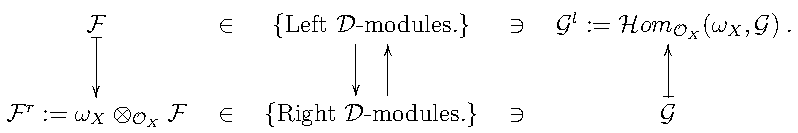
\includegraphics[width=0.6434\paperwidth]{images/L14-p117-leftright.pdf}\end{equation}
\end{figure}
$T_X$在$\omega_X\otimes_{\OO_X}\mathcal F$和$\mathcal Hom_{\OO_X}(\omega_X,\mathcal G)$上的作用分别为
\[(w\otimes u)\xi:=w\xi\otimes u-w\otimes\xi u,\qquad (\xi\varphi)(w):=\varphi(w\xi)-\varphi(w)\xi.\]
若$\mathcal G$为右D模，也称它为$\mathcal D^r$模；不加说明的D模始终指左D模。将$\mathcal D$自身视为右D模时，记为$\mathcal D^r$。

以$\mu(\mathcal D_X)$表示$\mathcal D_X$模的范畴，则有：
\originalnumber{6}
\begin{proposition}\label{L14S1O6}
$\mu(\mathcal D_X)$具有足够多的内射对象\znote{内射对象 $I$ 的性质是：对任意单射 $A\hookrightarrow B$ 与任意映射 $A\to I$，都存在 $B\to I$ 使之延拓。「足够多内射对象」意味着每个模都能嵌入某个内射模，这是 $\mathrm{RHom}$ 与导出范畴的整套同调代数能在 $\mu(\mathcal D_X)$ 中运作的前提；同调维数不超过 $2\dim_{\C}X$ 则说明可以用长度有界的复形计算导出函子。[来源：nLab 「injective object」，\url{https://ncatlab.org/nlab/show/injective+object}（Last revised 2025-12-24；2026-11-14 访问）。]}和局部投射对象，其同调维数有限，不超过$2\dim_{\C}X$。
\end{proposition}
\sourcepage{118}
可以类似地定义D模的导出范畴$D(\mathcal D_X)$。以$D^b(\mathcal D_X)$表示有界D模复形的导出范畴。
若D模$\mathcal F$作为$\OO_X$-模层局部自由，则有以下$\C_X$-线性复形：
\begin{equation}\tag{1.2}\label{L14eq12}
\operatorname{DR}_X(\mathcal F)=\bigl(\mathcal F\to\Omega_X^1\otimes\mathcal F\to\cdots\to\Omega_X^{d_X}\otimes\mathcal F\bigr)[d_X].
\end{equation}
% [Tutor Note: 原书 p118 作 $\Omega_X^{d_X-1}\otimes\mathcal F$，译文按 de Rham 复形的正确末项 $\Omega_X^{d_X}$ 处理。]
其中微分由\eref{引理}{L14S1O4}中D模结构对应的可积联络给出。\eqref{L14eq12}中的复形称为$\mathcal F$的\textbf{de Rham复形}，记为$\operatorname{DR}_X(\mathcal F)$。利用$\omega_X$的局部自由右$\mathcal D_X$-模消解，可得
\[\operatorname{DR}_X(\mathcal F)\cong\omega_X\overset{\mathrm L}{\otimes}_{\mathcal D_X}\mathcal F.\]
因此，对有界D模复形，可以定义
\[\operatorname{DR}_X(\mathcal F^\bullet):=\omega_X\overset{\mathrm L}{\otimes}_{\mathcal D_X}\mathcal F^\bullet.\]
我们将看到，将D模送到它的de Rham复形，正是实现Riemann--Hilbert对应的方式。\idx{de Rham复形}

\textbf{对偶化左D模}为
\[\mathcal D_X^\vee:=\mathcal Hom_{\OO_X}(\omega_X,\mathcal D_X^r),\]
即通过右左变换从$\mathcal D_X^r$得到的左模。对左D模$\mathcal F$，利用这一双模定义其对偶模
\[\mathcal F^\vee:=\mathcal Hom_{\mathcal D_X}(\mathcal F,\mathcal D_X^\vee).\]
在导出范畴中再加入平移$[d_X]$，得到对偶函子
\[\mathbb D_X(\mathcal F^\bullet):=\mathrm R\mathcal Hom_{\mathcal D_X}(\mathcal F^\bullet,\mathcal D_X^\vee)[d_X].\]
有
\begin{equation}\tag{1.3}\label{L14eq13}
\operatorname{DR}_X(\mathbb D_X(\mathcal F^\bullet))\cong\mathrm R\mathcal Hom_{\mathcal D_X}(\mathcal F^\bullet,\OO_X)[d_X].
\end{equation}
还可以定义逆像和直像。对复流形之间的全纯映射$f:X\to Y$，逆像的底层$\OO_X$-模为
\[f^*\mathcal G:=\OO_X\otimes_{f^{-1}\OO_Y}f^{-1}\mathcal G.\]
\sourcepage{119}
直像定义为
\[f_+\mathcal F:=f_*\mathcal F\otimes_{\mathcal D_X}f^*\mathcal D_Y.\]
$f^*$和$f_+$诱导导出范畴之间的函子，仍使用相同记号；此时$f^*$中的张量积也取导出张量积\znoteplain{原书此处未给出转移双模的显式写法；易错点是 $f_+$ 与 $f^!$ 的方向：$f_+$ 沿 $f$ 推前，把左 $\mathcal D_X$-模送到左 $\mathcal D_Y$-模，而 $f^!$ 形式上由 $\mathbb D$ 与 $f_+$ 复合给出，方向与 $f_+$ 相反，两者并非同一方向上的函子；套用公式前须先确认所引文献的左右模手性约定，否则平移与对偶会整体错位。（上下文推断，无外部依据）}。令$f^!:=f^*\circ[d_X-d_Y]$，再用对偶算子定义另外两个函子：
% [Tutor Note: 原书 p119 作 $f^!:=f^*\circ[d_Y-d_X]$，而 p124 的交换图按相反约定（由 $\operatorname{DR}_X(\OO_X)\cong\C_X[d_X]$ 验算，需平移 $[d_Y-d_X]$），二者互相矛盾，属原书内部约定不统一；译文统一取 $f^*[d_X-d_Y]$（与译文 $\mathbb D_X=\mathrm R\mathcal Hom(-,\mathcal D_X^\vee)[d_X]$ 的对偶约定自洽），读者引用时须按所引文献的约定换算。]
\[f^+:=\mathbb D_X\circ f^!\circ\mathbb D_Y,\qquad f_!:=\mathbb D_Y\circ f_+\circ\mathbb D_X.\]
\originalnumber{7}
\begin{theorem}[Kashiwara]\label{L14S1O7}
设$i:Z\to X$为非奇异流形之间的闭嵌入。令$\mu_Z(\mathcal D_X)$为$\mu(\mathcal D_X)$中由支撑包含于$Z$的$\mathcal D_X$模组成的满子范畴。
% [Tutor Note: 原书 p119 此处将 $\mu_Z(\mathcal D_X)$ 误作 $\mu_Z(\mathcal D_Z)$（它与「$\mu(\mathcal D_X)$ 的满子范畴」矛盾），译文按正确写法处理。]则函子
\[i_+:\mu(\mathcal D_Z)\to\mu_Z(\mathcal D_X),\qquad i^+:\mu_Z(\mathcal D_X)\to\mu(\mathcal D_Z)\]
互为逆函子，给出范畴等价。
\end{theorem}
\originalnumber{8}
\begin{note}[L14S1O8]
\eref{定理}{L14S1O7}还可以帮助我们定义奇异闭子簇$Z$上的D模范畴；此时$\mathcal D_Z$本身可能相当难处理。只需将$\mu(\mathcal D_Z)$定义为$\mu(\mathcal D_X)$的满子范畴$\mu_Z(\mathcal D_X)$。
\end{note}
\section{凝聚D模与完整D模}\label{L14S2}\idx{凝聚D模}\idx{完整D模}\idx{良滤过}\idx{特征簇}
若$\mathcal D_X$模$\mathcal F$局部有限表示，即局部有限生成，并且关系模也局部有限生成，则称它\textbf{凝聚}。换言之，在某个开集$U\subseteq X$上有正合列
\begin{equation}\tag{2.1}\label{L14eq21}
\mathcal D_X(U)^q\xrightarrow{\alpha}\mathcal D_X(U)^p\longrightarrow\mathcal F(U)\longrightarrow0.
\end{equation}
\originalnumber{1}
\begin{note}[L14S2O1]
凝聚$R$模$M$是一个有限生成模，并且任意有限组生成元之间的关系模也有限生成。因此，当$A$也凝聚时，任意满射$M^p\twoheadrightarrow A$的核都是有限生成的。

在代数几何的Noether情形中，对拟凝聚模而言，凝聚性就是局部有限生成性。但在解析几何中，局部有限生成并不等价于局部有限表示，因为关系核未必局部有限生成。
\sourcepage{120}
例如，在Noether代数几何中，结构层$\OO_X$的凝聚性是直接的；解析几何中的$\OO_X$也凝聚，但这是Oka的一个深刻定理。

$\OO_X$作为$\OO_X$-模凝聚这一很不平凡的事实，推出$\mathcal D_X$作为左$\mathcal D_X$模凝聚。因此，$\mathcal D_X$模的凝聚性等价于局部有限表示性。
\end{note}
以$\mu_{\mathrm{coh}}(\mathcal D_X)$表示$\mu(\mathcal D_X)$中由凝聚$\mathcal D_X$模组成的满子范畴。若D模复形的所有上同调层均凝聚，就称该复形凝聚。以$D_{\mathrm{coh}}^b(\mathcal D_X)$表示$D^b(\mathcal D_X)$中由凝聚D模复形组成的满子范畴。
\originalnumber{2}
\begin{proposition}\label{L14S2O2}
$\mu_{\mathrm{coh}}(\mathcal D_X)$是阿贝尔范畴，自然函子
\[D^b(\mu_{\mathrm{coh}}(\mathcal D_X))\longrightarrow D_{\mathrm{coh}}^b(\mathcal D_X)\]
为范畴等价。
\end{proposition}
一般而言，凝聚D模的逆像或直像未必凝聚。不过有：
\originalnumber{3}
\begin{proposition}\label{L14S2O3}
若$f:X\to Y$为真态射，则$f_+(D_{\mathrm{coh}}^b(\mathcal D_X))\subseteq D_{\mathrm{coh}}^b(\mathcal D_Y)$。
\end{proposition}
回忆$\mathcal D_X$的滤过
\begin{equation}\tag{2.2}\label{L14eq22}
\OO_X\cong F_0\mathcal D_X\subseteq\cdots\subseteq F_m\mathcal D_X\subseteq F_{m+1}\mathcal D_X\subseteq\cdots\subseteq\mathcal D_X=\bigcup_{m\ge0}F_m\mathcal D_X,
\end{equation}
其中$F_m\mathcal D_X$为阶数不超过$m$的算子层。它满足$F_m\mathcal D_X\cdot F_n\mathcal D_X\subseteq F_{m+n}\mathcal D_X$。相关分次代数层记为
\[\operatorname{Gr}^{\mathrm{ord}}\mathcal D_X:=\bigoplus_mF_m\mathcal D_X/F_{m-1}\mathcal D_X.\]
它是交换的，并自然同构于余切丛$\Omega_X^1$上沿纤维为多项式、沿底空间为全纯函数的函数层。这里用相同记号表示局部自由层及其对应的向量丛。

对任意D模$\mathcal F$，其\textbf{滤过}是一个$\OO_X$-子模序列
\[\cdots\subseteq\mathcal F_0\subseteq\mathcal F_1\subseteq\cdots\subseteq\mathcal F_m\subseteq\cdots\subseteq\mathcal F,\]
\sourcepage{121}
满足$\mathcal F=\bigcup_{m\in\Z}\mathcal F_m$，且对所有$m\in\N,n\in\Z$有$F_m\mathcal D_X(\mathcal F_n)\subseteq\mathcal F_{m+n}$。若分次模$\operatorname{Gr}^F\mathcal F:=\bigoplus_m\mathcal F_m/\mathcal F_{m-1}$还是凝聚的$\operatorname{Gr}^{\mathrm{ord}}\mathcal D_X$模，则称滤过为\textbf{良滤过}。这等价于下列两条件同时成立：
\begin{enumerate}[label=\arabic*.]
\item 对所有$m\ll0$，$\mathcal F_m=0$；对所有$r\gg0$，$F_1\mathcal D_X(\mathcal F_r)=\mathcal F_{r+1}$；
\item 每个$\mathcal F_m$都是凝聚$\OO_X$模。
\end{enumerate}
每个凝聚$\mathcal D_X$模都局部具有良滤过。有如下结论。
\originalnumber{4}
\begin{proposition}\label{L14S2O4}
设$(\mathcal F,F)$为带有良滤过的凝聚$\mathcal D_X$模，以$\mathcal I(\mathcal F,F)$表示$\operatorname{Gr}^F\mathcal F$在$\operatorname{Gr}^{\mathrm{ord}}\mathcal D_X$中的湮灭理想。则$\sqrt{\mathcal I(\mathcal F,F)}$不依赖于$\mathcal F$上良滤过$F$的选取。
\end{proposition}
\eref{命题}{L14S2O4}中的理想层$\sqrt{\mathcal I(\mathcal F,F)}$定义余切丛$\Omega_X^1$的一个子簇，称为$\mathcal F$的\textbf{特征簇}\znote{特征簇是余切丛中的子簇，记录 $\mathcal F$ 的「奇异方向」：当特征簇落在某点的零纤维内时，$\mathcal F$ 在该点附近作为 $\OO_X$-模局部自由，即没有奇性。它由理想层的根定义，因而总是既约的；对完整 D 模，它还是余切丛的 Lagrange 子簇。[来源：nLab 「holonomic D-module」，\url{https://ncatlab.org/nlab/show/holonomic+D-module}（Last revised 2014-02-16；2026-11-14 访问）；并见 Peters--Steenbrink, \textit{Mixed Hodge Structures}, Ch. 13 §13.3--§13.6（本讲参考文献）。]}，亦称\textbf{奇异支撑}，记为$\operatorname{Char}(\mathcal F)$。注意，它恰好是$\operatorname{Gr}^F\mathcal F$作为凝聚$\operatorname{Gr}^{\mathrm{ord}}\mathcal D_X$模的支撑$\operatorname{Supp}(\operatorname{Gr}^F\mathcal F)\subseteq\Omega_X^1$。

一般很难描述逆像、直像的特征簇。$f_+,f^*$通常不保持D模的凝聚性。不过，对闭嵌入和光滑态射，有以下结果。
\begin{enumerate}[label=(\roman*)]
\item 若$i:Z\to X$为非奇异流形之间的闭嵌入，则对任意$\mathcal D_Z$模$\mathcal F$，$i_+\mathcal F$凝聚当且仅当$\mathcal F$凝聚。此外，
\[\operatorname{Char}(i_+\mathcal F)=\{(x,\xi)\mid x\in Z,\ (x,\operatorname{Pr}^{\Omega}(\xi))\in\operatorname{Char}(\mathcal F)\},\]
其中$\operatorname{Pr}^{\Omega}:\Omega_X^1|_Z\to\Omega_Z^1$为限制映射。
\item 若$\pi:Y\to X$为光滑态射，则微分给出映射$d\pi:\pi^*\Omega_X^1\to\Omega_Y^1$。对任意$\mathcal D_X$模$\mathcal G$，$\pi^*\mathcal G$凝聚当且仅当$\mathcal G$凝聚。此外，
\[\operatorname{Char}(\pi^*\mathcal G)=\{(y,\xi)\mid y\in Y,\ \xi=d\pi(\eta),\ (\pi(y),\eta)\in\operatorname{Char}(\mathcal G)\}.\]
\end{enumerate}
\originalnumber{5}
\begin{theorem}\label{L14S2O5}
若$\mathcal F\ne0$为凝聚$\mathcal D_X$模，则$\dim_{\C}\operatorname{Char}(\mathcal F)\ge\dim_{\C}X$。
\end{theorem}
\sourcepage{122}
\originalnumber{6}
\begin{definition}\label{L14S2O6}
若凝聚$\mathcal D_X$模$\mathcal F\ne0$满足$\dim_{\C}\operatorname{Char}(\mathcal F)=\dim_{\C}X$，则称它为\textbf{完整模}\znote{完整（holonomic）是 D 模理论中最基本的有穷性条件：它要求 $\mathcal F$ 凝聚，且特征簇不可再小（维数恰为 $\dim X$），等价地，特征簇是余切丛的 Lagrange 子簇。完整 D 模的解空间局部有限维，这正是 Riemann--Hilbert 对应能把它与反常层这样的有限维数据对应起来的原因。[来源：nLab 「holonomic D-module」，\url{https://ncatlab.org/nlab/show/holonomic+D-module}（Last revised 2014-02-16；2026-11-14 访问）；并见 J. Bernstein, \textit{Algebraic Theory of D-modules}（本讲参考文献 [B]）。]}。零模也约定为完整模。
\end{definition}
\originalnumber{7}
\begin{example}\label{L14S2O7}
\begin{enumerate}[label=(\arabic*)]
\item 任意凝聚$\OO_X$模$\mathcal F$若具有D模结构，便是完整$\mathcal D_X$模。因为平凡滤过是良滤过，$\operatorname{Char}(\mathcal F)$等于其支撑上的零截面；在$X$连通且$\mathcal F\ne0$时，支撑为$X$，参见\eref{笔记}{L14S1O5}。事实上，任意具有D模结构的凝聚$\OO_X$模都局部自由。
\item 若$i:Z\to X$为非奇异流形之间的闭嵌入，$\mathcal F$为具有$\mathcal D_Z$-模结构的非零凝聚$\OO_Z$模，则$i_+\mathcal F$完整，其特征簇是$Z$的余法丛。
\end{enumerate}
\end{example}
以$D_h^b(\mathcal D_X)$表示$D_{\mathrm{coh}}^b(\mathcal D_X)$中由上同调层均为完整模的有界复形组成的满子范畴。注意，完整D模复形的各项未必都是完整模；要求完整的只是它的上同调层。
\originalnumber{8}
\begin{proposition}\label{L14S2O8}
\begin{enumerate}[label=(\arabic*)]
\item 若$f:X\to Y$为真全纯映射，则$f_+$保持完整复形，并给出
\[f_+:D_h^b(\mathcal D_X)\to D_h^b(\mathcal D_Y).\]
此外，$\mathbb D_Y\circ f_+\cong f_+\circ\mathbb D_X$。
% [Tutor Note: 原书 p122 将 $\mathbb D_Y\circ f_+\cong f_+\circ\mathbb D_X$ 误作 $\mathbb D_X\circ f_+\cong f_+\circ\mathbb D_X$，译文按正确写法处理。]
\item 若$f:X\to Y$为全纯映射，则导出逆像保持完整性，并给出
\[f^!:D_h^b(\mathcal D_Y)\to D_h^b(\mathcal D_X).\]

\end{enumerate}
\end{proposition}
\originalnumber{9}
\begin{theorem}\label{L14S2O9}
设$\mathcal F^\bullet$为有界$\mathcal D_X$-模复形。它完整，当且仅当它凝聚，且对任意$x\in X$，其在$x$处的导出纤维$i_x^!\mathcal F^\bullet$的各个上同调空间都有限维。
\end{theorem}
\section{Riemann--Hilbert对应}\label{L14S3}\idx{Riemann--Hilbert对应}\idx{正则完整D模}\idx{解复形}
\originalnumber{1}
\begin{theorem}[Kashiwara]\label{L14S3O1}
设$X$为复解析流形。完整$\mathcal D_X$模的de Rham复形为反常层。
\end{theorem}
\sourcepage{123}
对任意$u=(u_1,\ldots,u_p)\in\OO_X(U)^p\subseteq\mathcal D_X(U)^p$，定义映射
\[\varphi_u:\mathcal D_X(U)^p\longrightarrow\OO_X(U),\qquad (P_1,\ldots,P_p)\longmapsto\sum_{j=1}^pP_j(u_j).\]
% [Tutor Note: 原书 p123 作 $(P_1,\ldots,P_q)\mapsto\sum_{j=1}^qP_j(u_j)$，与定义域 $\mathcal D_X(U)^p$ 不符，译文统一为 $p$。]
映射$\varphi_u$经由\eqref{L14eq21}中的$\mathcal F(U)$分解，当且仅当$\alpha^T(u)=0$；这里$\alpha^T$是在$\mathcal D_X(U)^p$、$\mathcal D_X(U)^q$的标准基下，由$\alpha$的转置矩阵给出的微分算子作用。因此有一一对应
\[\ker\bigl(\alpha^T:\OO_X(U)^p\to\OO_X(U)^q\bigr)\xleftrightarrow{1\text{--}1}\operatorname{Sol}(\mathcal F(U)):=\Hom_{\mathcal D_X(U)}(\mathcal F(U),\OO_X(U)).\]
\originalnumber{2}
\begin{definition}\label{L14S3O2}
设$\mathcal F$为凝聚$\mathcal D_X$模，其\textbf{解层}为复向量空间层
% [Tutor Note: 原书 p123 称 $\operatorname{Sol}(\mathcal F)$ 为「the $D_X$-module」，实为复向量空间层，译文按正确写法处理。]
\[\operatorname{Sol}(\mathcal F):=\mathcal Hom_{\mathcal D_X}(\mathcal F,\OO_X).\]
在凝聚D模有界复形的导出范畴$D_{\mathrm{coh}}^b(\mathcal D_X)$中，定义\textbf{解复形}
\begin{equation}\tag{3.1}\label{L14eq31}
\operatorname{Sol}(\mathcal F^\bullet):=\mathrm R\mathcal Hom_{\mathcal D_X}(\mathcal F^\bullet,\OO_X)[d_X]\cong\operatorname{DR}_X(\mathbb D_X\mathcal F^\bullet),
\end{equation}
其中第二个同构来自\eqref{L14eq13}。
\end{definition}
设$X$为复代数流形。如果对光滑不可约曲线$C$到$X$的任意代数态射$u:C\to X$，完整复形$u^!\mathcal F^\bullet$在$C$上都是正则完整的，则称完整复形$\mathcal F^\bullet$\textbf{正则完整}。在曲线上，正则性意味着各个上同调D模在光滑部分对应的联络仅有正则奇点；对代数曲线，也包括光滑完备化的边界点。以$D_{rh}^b(\mathcal D_X)$表示$D_h^b(\mathcal D_X)$中由有界正则完整复形组成的满子范畴。由\eref{定理}{L14S3O1}和下面的Riemann--Hilbert对应，每个完整复形的de Rham复形，都与一个唯一的正则完整复形的de Rham复形同构。
\originalnumber{3}
\begin{theorem}[Riemann--Hilbert对应II]\label{L14S3O3}
设$X$为复代数流形。
\begin{enumerate}[label=\arabic*.]
\item de Rham函子
\[\operatorname{DR}_X:D_{rh}^b(\mathcal D_X)\longrightarrow D_c^b(\C_X),\qquad\mathcal F^\bullet\longmapsto\operatorname{DR}_X(\mathcal F^\bullet),\]
是范畴等价，其中右侧取$X$的解析拓扑及代数可构造上同调。在这一等价下，正则完整$\mathcal D_X$模恰好对应于复系数反常层。
\sourcepage{124}
\item 在de Rham等价下，以$\mathbb D_X^V$表示的Verdier对偶与\eqref{L14eq13}中的D模对偶$\mathbb D_X$相对应，即
\[\operatorname{DR}_X\circ\mathbb D_X\cong\mathbb D_X^V\circ\operatorname{DR}_X.\]
特别地，任意正则完整复形的\eqref{L14eq31}所定义的解复形，是其de Rham复形的Verdier对偶：
\[\operatorname{Sol}(\mathcal F^\bullet)\cong\mathbb D_X^V(\operatorname{DR}_X(\mathcal F^\bullet)).\]
\item 若$f:X\to Y$为光滑复代数簇之间的态射，则有以下两个交换图：
\begin{figure}[H]\centering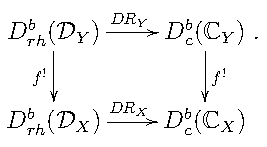
\includegraphics[width=0.2152\paperwidth]{images/L14-p124-pullback.pdf}\end{figure}
\begin{figure}[H]\centering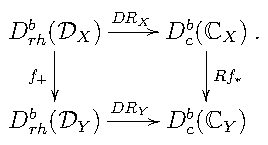
\includegraphics[width=0.2162\paperwidth]{images/L14-p124-direct.pdf}\end{figure}
特别地，即使$f$不是真映射，$\mathrm Rf_*$仍保持代数可构造性。
\end{enumerate}
\end{theorem}
\needspace{5\baselineskip}\section{第14讲参考文献}\label{L14S4}
\begin{references}
\refitem{L14bibPS}{PS} Chris A. M. Peters and Joseph H. M. Steenbrink, \emph{Mixed Hodge Structures}, Springer-Verlag Berlin Heidelberg, Ch. 13 \S13.3--\S13.6.
\refitem{L14bibB}{B} J. Bernstein, \emph{Algebraic Theory of D-modules}, available at\\ \url{http://www.math.columbia.edu/~khovanov/resources/Bernstein-dmod.pdf}.
\end{references}

\chapter{几何阿贝尔类域论}\label{L15}\lecturedate{2020/04/08}\sourcepage{125}
本讲讨论$n=1$时的几何Langlands对应。这一情形相当简单，也已经得到充分理解。

设$X$为$\F_q$或$\C$上的光滑射影曲线。回忆，Langlands对应的几何重述断言存在以下单向映射：
\begin{figure}[H]\centering\begin{equation}\tag{0.1}\label{L15eq01}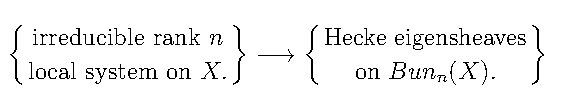
\includegraphics[width=0.4657\paperwidth]{images/L15-p125-correspondence.pdf}\end{equation}\end{figure}
设$E_\sigma$为$X$上对应于表示$\sigma:\widehat\pi_1(X)\to\GL_n(\overline{\Q}_\ell)$的$\overline{\Q}_\ell$局部系统。若对每个$i=1,\ldots,n$，均存在同构
\begin{equation}\tag{0.2}\label{L15eq02}T^i(\mathcal F_\sigma)\cong\bigwedge^iE_\sigma\boxtimes\mathcal F_\sigma,\end{equation}
则称$\mathcal F_\sigma\in D_c^b(\operatorname{Bun}_n(X))$为相对于$\sigma$的Hecke特征层，其中$\bigwedge^i$表示第$i$次外幂。

现在令$n=1$。首先，将线丛模叠$\operatorname{Bun}_1(X)$的标量自同构刚性化\znoteplain{线丛模叠的每个对象都带有 $\C^\times$ 的标量自同构，因此它是 $\operatorname{Pic}(X)$ 上的 $\C^\times$-gerbe，而不是概形。刚性化就是把这些标量自同构固定下来（等价于把该 gerbe 平凡化），从而得到 Picard 概形。同样的说法在§3 用于局部系统：刚性化的一维局部系统指附带一个固定同构 $\psi:\mathcal A_L|_0\cong\overline{\Q}_\ell$，即指定了基点处纤维的一个标架。（上下文推断，无外部依据）}，得到$X$的Picard概形$\operatorname{Pic}(X)$。其次，只需考虑Hecke算子$T^1$。于是\eqref{L15eq02}中的Hecke特征层条件简化为
\begin{equation}\tag{0.3}\label{L15eq03}T^1(\mathcal F_\sigma)\cong E_\sigma\boxtimes\mathcal F_\sigma.\end{equation}
我们将看到，$X$上的一维$\ell$进局部系统$E_\sigma$对应的Hecke特征对象$\mathcal F_\sigma$实际上是一个层，而非多项复形。此外，在$n=1$时，这些Hecke特征层可以由内在性质定义，而不必先涉及$X$上的$\ell$进局部系统；\eqref{L15eq01}的映射此时为双射。
\sourcepage{126}
\section{\texorpdfstring{$n=1$时的Hecke算子$T^1$}{n=1时的Hecke算子T¹}}\label{L15S1}
一个标准事实是：若$F$为可分闭域，则$\widehat\pi_1(\mathbb P_F^n,\overline x)=1$。可以假设曲线$X$在几何上不是$\mathbb P^1$，因而$g(X)\ge1$。
\originalnumber{1}
\begin{lemma}\label{L15S1O1}
设$X$为$k$上的光滑射影几何连通曲线，且$g(X)\ge1$。则$X$上不同的$k$-点$x_1,x_2$不可能线性等价，即
\[\OO_X(x_1)\cong\OO_X(x_2)\quad\Longleftrightarrow\quad x_1=x_2.\]
\end{lemma}
\begin{proof}
若$x_1,x_2$不同却线性等价，则存在$f\in K(X)$，满足$\operatorname{div}(f)=x_1-x_2$，特别地，$f(x_1)=0$、$f(x_2)=\infty$。有理函数$f$诱导态射$f:X\to\mathbb P^1$，其次数为一，因为零点除子恰为$x_1$。这与$g(X)\ge1$矛盾。
\end{proof}
回忆，第$i$个Hecke对应$\mathcal H^i$参数化四元组$(\mathcal M,\mathcal M',x,\beta:\mathcal M\hookrightarrow\mathcal M')$。当$n=1$时，只有第一个Hecke对应$\mathcal H^1$及以下三个映射：
\begin{figure}[H]\centering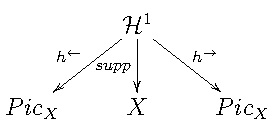
\includegraphics[width=0.2222\paperwidth]{images/L15-p126-Hecke.pdf}\end{figure}
它们满足下图所示的关系：
\begin{figure}[H]\centering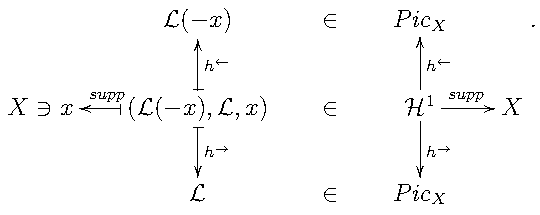
\includegraphics[width=0.4354\paperwidth]{images/L15-p126-maps.pdf}\end{figure}
由\eref{引理}{L15S1O1}及线丛修改的描述可知$\mathcal H^1\cong\operatorname{Pic}_X\times X$，且$\operatorname{supp}\times h^\rightarrow$为同构。Hecke函子写为
\[T^i(\mathcal K^\bullet)=(\operatorname{supp}\times h^\rightarrow)_*(h^\leftarrow)^{-1}(\mathcal K^\bullet)[i(n-i)].\]
因此，当$n=1$时，在以$\operatorname{supp}\times h^\rightarrow$识别两个空间后，$T^1$就是沿加点映射的逆像。更确切地说，以$\operatorname{Pic}_X^d$表示$\operatorname{Pic}_X$中参数化次数$d$线丛的分支，以$\mathcal F^d$表示层$\mathcal F$在该分支上的限制。
\sourcepage{127}
于是\eqref{L15eq03}中的Hecke特征层条件变为
\begin{equation}\tag{1.1}\label{L15eq11}m_X^{-1}(\mathcal F_\sigma^{d+1})\cong\mathcal F_\sigma^d\boxtimes L_\sigma,\end{equation}
其中$L_\sigma=E_\sigma$为表示$\sigma$所对应的局部系统，$m_X:\operatorname{Pic}_X^d\times X\to\operatorname{Pic}_X^{d+1}$为$(\mathcal L,x)\mapsto\mathcal L(x)$。
\section{曲线的对称幂}\label{L15S2}\idx{对称幂}\idx{Abel--Jacobi映射}
仍设$X$为域$k$上的光滑曲线。以$X^{(d)}$表示$X$的第$d$个对称幂\znote{$d$ 次对称幂首先是对向量空间定义的：$\operatorname{Sym}^dV$ 是 $d$ 重张量幂对 $\mathfrak S_d$ 置换作用的商，特征为零时可等同于不变张量。本讲的 $X^{(d)}$ 是同一构造在曲线上的几何版本：它参数化 $d$ 次有效除子 $x_1+\cdots+x_d$，即 $X^d$ 对 $\mathfrak S_d$ 的商。常见误解是「取商必生奇点」，但 $d\ge1$ 时 $X^{(d)}$ 仍然光滑（命题 2.2）。[来源：MathWorld 词条「Symmetric Power（对称幂）」，\url{https://mathworld.wolfram.com/SymmetricPower.html}（2026-11-14 访问）。]}，以$X^d$表示其$d$重乘积，则有仿射的商映射
\[\pi^d:X^d\longrightarrow X^{(d)}.\]
以$\mathfrak S_d$表示$d$次对称群，则$X^{(d)}\cong X^d/\!/\mathfrak S_d$。有一个自然的\textbf{Abel--Jacobi映射}\znote{经典情形下，$\operatorname{Div}^0(X)\to J(X)$ 由积分定义，Abel 定理说其核恰为主除子，于是它把除子的线性等价类实现为 Jacobian 簇中的点。$AJ_d$ 是它在 $d$ 次有效除子上的版本：$X^{(d)}$ 参数化 $d$ 次有效除子，$AJ_d$ 把它们送到 $\operatorname{Pic}_X^d$；由 Abel 定理，纤维正是同一线性等价类的全部有效除子，即完备线性系，故当 $d\ge2g-1$ 时纤维是射影空间（命题 2.5）。[来源：nLab 「Abel-Jacobi map」，\url{https://ncatlab.org/nlab/show/Abel-Jacobi+map}（Last revised 2023-06-09；2026-11-14 访问）。]}：
\begin{equation}\tag{2.1}\label{L15eq21}
AJ_d:X^{(d)}\longrightarrow\operatorname{Pic}_X^d,\qquad (x_1,\ldots,x_d)\longmapsto\OO_X(x_1+\cdots+x_d).
\end{equation}
\originalnumber{1}
\begin{note}[L15S2O1]
\eqref{L15eq21}中的$AJ_d$不仅是集合论映射，还是代数概形之间的态射，因为它来自相应函子之间的自然变换。
\end{note}
对两个正整数$d,e$，同构$X^d\times X^e\xrightarrow{\sim}X^{d+e}$诱导典范态射
\begin{equation}\tag{2.2}\label{L15eq22}\widetilde m_{d,e}:X^{(d)}\times X^{(e)}\longrightarrow X^{(d+e)}.\end{equation}
\originalnumber{2}
\begin{proposition}\label{L15S2O2}
当$d\ge1$时，$X^{(d)}$非奇异。
\end{proposition}
\begin{proof}
只需证明：对任意几何闭点$y\in X^{(d)}$，局部环$\OO_{X^{(d)},y}$的极大理想$\mathfrak m_y$可由不超过$d$个元素生成。由\eqref{L15eq22}，只需考虑$y=(x,x,\ldots,x)$的情形，其中$x\in X$。还可以将局部环换成其完备化$\widehat{\OO}_{X^{(d)},y}$。设$\widetilde y$为$y$在$X^d$中的原像，则
\[\widehat{\OO}_{X^{(d)},y}\cong(\widehat{\OO}_{X^d,\widetilde y})^{\mathfrak S_d}.\]
另一方面，在代数闭的剩余域上，$\widehat{\OO}_{X^d,\widetilde y}\cong\overline k[[t_1,\ldots,t_d]]$，且此同构将$\mathfrak m_{\widetilde y}$对应到$\langle t_1,\ldots,t_d\rangle$。
\sourcepage{128}
因而，在不变量环中有
\[\mathfrak m_y=\mathfrak m_{\widetilde y}\cap(\widehat{\OO}_{X^d,\widetilde y})^{\mathfrak S_d}\cong\langle\sigma_1,\ldots,\sigma_d\rangle,\]
其中$\sigma_j$为变量$t_1,\ldots,t_d$的第$j$个初等对称多项式。因此$\mathfrak m_y$可由$d$个元素生成，命题得证。
\end{proof}
设$L$为$X$上的一维$\ell$进局部系统。定义$L^{\boxtimes d}:=\bigotimes_{j=1}^d\operatorname{pr}_j^{-1}L$，其中$\operatorname{pr}_j:X^d\to X$为第$j$个因子的投影。于是$L^{\boxtimes d}$是$X^d$上的一维$\ell$进局部系统，带有$\mathfrak S_d$-线性化：对每个$\sigma\in\mathfrak S_d$及$(x_1,\ldots,x_d)\in X^d$，有同构
\[h_{(x_1,\ldots,x_d),\sigma}:\bigotimes_{j=1}^dL_{x_j}\xrightarrow{\sim}\bigotimes_{j=1}^dL_{x_{\sigma(j)}}.\]
\originalnumber{3}
\begin{proposition}\label{L15S2O3}
$L^{\boxtimes d}$下降为$X^{(d)}$上的一维$\ell$进局部系统$L^{(d)}$。
\end{proposition}
\begin{proof}
令$L^{(d)}:=(\pi_*L^{\boxtimes d})^{\mathfrak S_d}$，其中$\pi=\pi^d:X^d\to X^{(d)}$为商映射。只需证明$\pi^{-1}L^{(d)}\cong L^{\boxtimes d}$。注意，对态射$f:X\to Y$和$X$上的平展层$\mathcal F$，有自然映射$f^{-1}f_*\mathcal F\to\mathcal F$，因此得到
\begin{figure}[H]\centering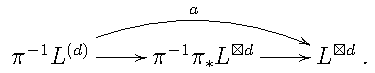
\includegraphics[width=0.3020\paperwidth]{images/L15-p128-descent.pdf}\end{figure}
由可构造层的真基变换性质，即\eref{定理}{L13S2O4}，映射$a:\pi^{-1}L^{(d)}\to L^{\boxtimes d}$在每个茎上均为同构，因而本身为同构。
\end{proof}
有以下交换图：
\begin{figure}[H]\centering\begin{equation}\tag{2.3}\label{L15eq23}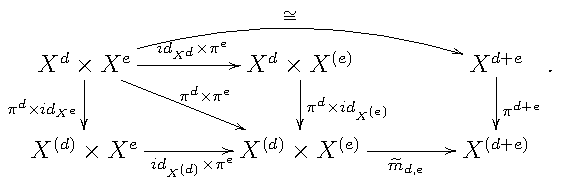
\includegraphics[width=0.4616\paperwidth]{images/L15-p128-symmetric.pdf}\end{equation}\end{figure}
\originalnumber{4}
\begin{proposition}\label{L15S2O4}
$\widetilde m_{d,e}^{-1}L^{(d+e)}\cong L^{(d)}\boxtimes L^{(e)}$。
\end{proposition}
\begin{proof}
由$X^d\times X^e\cong X^{d+e}$，有$L^{\boxtimes d}\boxtimes L^{\boxtimes e}\cong L^{\boxtimes(d+e)}$。由\eqref{L15eq23}，
\[\begin{aligned}
(\pi^d)^{-1}L^{(d)}\boxtimes(\pi^e)^{-1}L^{(e)}&\cong L^{\boxtimes(d+e)}\\
&\cong(\pi^{d+e})^{-1}L^{(d+e)}\\
&\cong(\pi^d\times\pi^e)^{-1}\widetilde m_{d,e}^{-1}L^{(d+e)}.
\end{aligned}\]
\sourcepage{129}
因此$\widetilde m_{d,e}^{-1}L^{(d+e)}\cong L^{(d)}\boxtimes L^{(e)}$，因为二者都是局部系统$L^{\boxtimes d}\boxtimes L^{\boxtimes e}$的相容下降。
\end{proof}
注意$X^{(1)}\cong X^1\cong X$，且$L^{(1)}\cong L$。因此$L^{(d)}$满足与\eqref{L15eq11}类似的Hecke特征层性质：
\begin{equation}\tag{2.4}\label{L15eq24}\widetilde m_{d,1}^{-1}L^{(d+1)}\cong L^{(d)}\boxtimes L.\end{equation}
由Riemann--Roch定理可以得到以下命题。
\originalnumber{5}
\begin{proposition}\label{L15S2O5}
设$g=g(X)\ge1$。若$d\ge2g-1$，则\eqref{L15eq21}中的Abel--Jacobi映射$AJ_d$为真满射，其在几何点$\Spec\Omega\to\operatorname{Pic}_X^d$处的几何纤维同构于射影空间$\mathbb P_\Omega^{d-g}$。
\end{proposition}
\section{Deligne的几何证明}\label{L15S3}\idx{几何阿贝尔类域论}\idx{乘法局部系统}
假设$X$有一个$k$-有理点$p$。我们要证明以下定理。
\originalnumber{1}
\begin{theorem}[Deligne]\label{L15S3O1}
以下两类对象的同构类一一对应：
\begin{figure}[H]\centering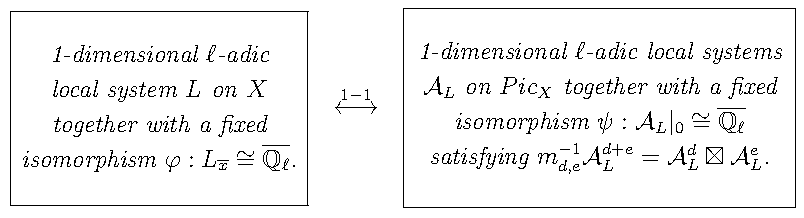
\includegraphics[width=0.6485\paperwidth]{images/L15-p129-Deligne.pdf}\end{figure}
这里$\mathcal A_L^d$为$\mathcal A_L$在分支$\operatorname{Pic}_X^d$上的限制，$m_{d,e}:\operatorname{Pic}_X^d\times\operatorname{Pic}_X^e\to\operatorname{Pic}_X^{d+e}$为线丛张量积诱导的自然映射。
\end{theorem}
\begin{proof}
给定一维$\ell$进局部系统$L$、几何点$x:\operatorname{Spec}\Omega\to X$\znoteplain{此处 $x$ 指几何点 $\operatorname{Spec}\Omega\to X$，与本节构造里用到的 $k$-有理点 $p$ 不是一类对象：$x$ 的剩余域是代数闭包 $\Omega$，只在取纤维 $L_{\bar x}$ 时出现；而 $p\in X(k)$ 才能用来把 $\mathcal A_L^d$ 沿 $dp$ 标架化。原书混用这两个记号，阅读时按 $L_{\bar x}$ 的下标理解即可。（上下文推断，无外部依据）}及固定同构$\varphi:L_{\overline x}\cong\overline{\Q}_\ell$，可以在$X^{(d)}$上构造一维$\ell$进局部系统$L^{(d)}$，它对应于Galois表示
\[\rho_{L^{(d)}}:\widehat\pi_1(X^{(d)})\longrightarrow\overline{\Q}_\ell^{\times}.\]
该表示经由阿贝尔化$\widehat\pi_1(X^{(d)})\to\widehat\pi_1^{\mathrm{ab}}(X^{(d)})$分解。
\sourcepage{130}
现在设$d\ge2g(X)-1$。由\eref{定理}{L10S3O1}及\eref{命题}{L15S2O5}，有正合列
\[\widehat\pi_1(\mathbb P_\Omega^{d-g},\overline x)\longrightarrow\widehat\pi_1(X^{(d)},\overline x)\longrightarrow\widehat\pi_1(\operatorname{Pic}_X^d,\overline{AJ_d(x)})\longrightarrow1.\]
由于$\widehat\pi_1(\mathbb P_\Omega^{d-g},\overline x)$平凡，$AJ_d$诱导基本群同构。因此$\widehat\pi_1(X^{(d)},\overline x)$的每个一维表示都诱导$\widehat\pi_1(\operatorname{Pic}_X^d,\overline{AJ_d(x)})$的唯一一维表示。于是，在$\operatorname{Pic}_X^d$上有唯一的一维$\ell$进局部系统$\mathcal A_L^d$，带有固定同构$\psi:\mathcal A_L^d|_{dp}\cong\overline{\Q}_\ell$，满足$AJ_d^{-1}\mathcal A_L^d\cong L^{(d)}$。

此外有下列交换图：
\begin{figure}[H]\centering\begin{equation}\tag{3.1}\label{L15eq31}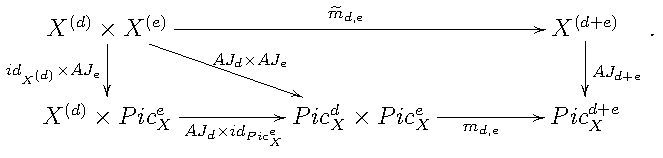
\includegraphics[width=0.5343\paperwidth]{images/L15-p130-tensor.pdf}\end{equation}\end{figure}
若$d,e\ge2g(X)-1$，由\eref{命题}{L15S2O4}可得$m_{d,e}^{-1}\mathcal A_L^{d+e}\cong\mathcal A_L^d\boxtimes\mathcal A_L^e$。

我们已经在$d\ge2g(X)-1$的分支$\operatorname{Pic}_X^d$上定义了$\mathcal A_L^d$，接下来要对所有$d\in\Z$构造它。利用\eqref{L15eq31}的交换图，令$e=1$，并选取$k$-有理点$p\in X$，有
\[\operatorname{Pic}_X^d\cong\{p\}\times\operatorname{Pic}_X^d\overset{i_p}{\hookrightarrow}X\times\operatorname{Pic}_X^d\xrightarrow{m_X}\operatorname{Pic}_X^{d+1}.\]
定义
\begin{equation}\tag{3.2}\label{L15eq32}\mathcal A_L^d:=i_p^{-1}m_X^{-1}(\mathcal A_L^{d+1})\otimes L_{\overline p}^{\vee}.\end{equation}
可以检验，以此方式定义的$\mathcal A_L$为$\operatorname{Pic}_X$上的一维$\ell$进局部系统，具有单位元处的固定同构$\psi:\mathcal A_L|_0\cong\overline{\Q}_\ell$，并满足$m_{d,e}^{-1}\mathcal A_L^{d+e}\cong\mathcal A_L^d\boxtimes\mathcal A_L^e$。

反过来，设$\mathcal A_L$为$\operatorname{Pic}_X$上刚性化的一维乘法$\ell$进局部系统。考虑Abel--Jacobi映射$AJ_1:X\to\operatorname{Pic}_X^1$。
\sourcepage{131}
其逆像$AJ_1^{-1}\mathcal A_L^1$为$X$上的一维$\ell$进局部系统；选取在$\overline p$处的标架后，它也具有刚性化。证明上述两个构造在同构类层面互为逆构造，留给读者。
\end{proof}
\originalnumber{2}
\begin{note}[L15S3O2]
若$k=\C$，则$\operatorname{Pic}_X^0$为$X$的Jacobian簇，且
\[\operatorname{Pic}_X^0\cong H^1(X,\OO_X)/H^1(X,\Z).\]
其平展基本群为阿贝尔群，且
\[\widehat\pi_1(\operatorname{Pic}_X^0)\cong\widehat{H_1(\operatorname{Pic}_X^0,\Z)}\cong\widehat{H_1(X,\Z)}\cong\widehat\pi_1^{\mathrm{ab}}(X).\]
这里帽号表示射有限完备化\znote{设 $N$ 取遍 $G$ 的有限指数正规子群，$G$ 的射有限完备化 $\widehat G$ 就是有限商 $G/N$ 在自然投影下的逆向极限；它是紧、Hausdorff、全不连通的拓扑群，而射有限群正是有限群的逆向极限。Galois 理论中的绝对 Galois 群与 étale 基本群天然是这种群，所以这里的「一维表示」须理解为取值于 $\overline{\Q}_\ell^\times$ 的连续同态，正因如此才能用有限层的同调来计算。[来源：nLab 「profinite group」，\url{https://ncatlab.org/nlab/show/profinite+group}（Last revised 2025-07-01；2026-11-14 访问）。]}。表示$\rho:\widehat\pi_1(X)\to\overline{\Q}_\ell^{\times}$经由$\widehat\pi_1(X)\to\widehat\pi_1^{\mathrm{ab}}(X)$分解。由Poincaré对偶，$H_1(X,\Z)$与$H^1(X,\Z)$典范对应。因此，$\widehat\pi_1(X)$的一维表示诱导$\widehat\pi_1(\operatorname{Pic}_X^0)$的唯一一维表示，可以将$L$对应到$\operatorname{Pic}_X^0$上的唯一局部系统$\mathcal A_L^0$。

再用递归公式\eqref{L15eq32}定义所有$d\le0$时的$\mathcal A_L^d$。当$d>0$时，有同构
\begin{figure}[H]\centering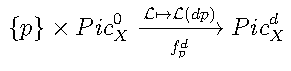
\includegraphics[width=0.2343\paperwidth]{images/L15-p131-translation.pdf}\end{figure}
并定义$\mathcal A_L^d\cong(f_p^d)_*(\mathcal A_L^0\otimes L_{\overline p}^{\otimes d})$。构造$L\leftrightarrow\mathcal A_L$实现了\eref{定理}{L15S3O1}中的一一对应。
\end{note}
\needspace{5\baselineskip}\section{第15讲参考文献}\label{L15S4}
\begin{references}
\refitem{L15bibT}{T} Péter Tóth, \emph{Geometric abelian class field theory}, Thesis for MD at Univ. Utrecht, available at \url{http://math.bu.edu/people/magner/Seminar/GCFTthesis.pdf}.
\refitem{L15bibL}{L} G. Laumon, \emph{Faisceaux Automorphes Lies aux Series Eisenstein}, In L. Clozel and J.S. Milne, editors, \emph{Automorphic Forms, Shimura Varieties and L-functions}, Academic Press, 1990.
\refitem{L15bibH}{H} J. Heinloth, \emph{Class field theory}, in \emph{Geometric Langlands Program winter school in Göttingen}, 2007.
\end{references}

\chapter{几何形式的Artin互反律}\label{L16}\lecturedate{2020/04/13}\sourcepage{132}
上一讲介绍了几何阿贝尔类域论。回忆，在\lref{L2}和\lref{L3}中，我们已经介绍Artin映射和Artin互反律。本讲讨论Artin互反律的几何形式，并利用Deligne关于Langlands对应的几何构造来证明它。
\section{Artin映射与Artin互反律}\label{L16S1}
先回顾数论情形中的Artin映射和Artin互反律。设$F$为代数数域，$\OO_F$为其代数整数环。设$L/F$为有限Galois扩张，$D$为$\OO_F$在$L$中的整闭包；$\Pp$为$D$中的素理想，位于$\OO_F$的素理想$\p$之上。$\Pp$的分解群为
\[G_{\Pp}=\{\sigma\in\Gal(L/F)\mid\sigma\Pp=\Pp\}.\]
以$L_{\Pp}$、分别$F_{\p}$表示$L$、分别$F$关于素理想$\Pp$、分别$\p$的完备化。则$L_{\Pp}/F_{\p}$也是有限Galois扩张，每个$\sigma\in G_{\Pp}$都诱导$L_{\Pp}$的$F_{\p}$-自同构，因此有映射$i:G_{\Pp}\to\Gal(L_{\Pp}/F_{\p})$。由\eref{命题}{L3S1O2}，它是同构，所以可以将$\Gal(L_{\Pp}/F_{\p})$视为$\Gal(L/F)$的子群。

剩余域$D/\Pp$是$\OO_F/\p$的有限Galois扩张。自然限制映射
\[\Gal(L_{\Pp}/F_{\p})\longrightarrow\Gal((D/\Pp)/(\OO_F/\p))\]
为满射，参见\eref{命题}{L2S2O3}。
\sourcepage{133}
复合映射$G_{\Pp}\xrightarrow{\sim}\Gal(L_{\Pp}/F_{\p})\to\Gal((D/\Pp)/(\OO_F/\p))$的核，称为$\Pp$的\textbf{惯性群}，记为$I_{\Pp}$。若$L_{\Pp}/F_{\p}$非分歧，等价地，$\p$在$L$中非分歧，则$I_{\Pp}=\{1\}$。此时定义$\Pp$处的\textbf{Frobenius元素}为$\Gal((D/\Pp)/(\OO_F/\p))\cong\Gal(\F_{q^f}/\F_q)$中算术Frobenius自同构的唯一原像，记为$\mathrm{Fr}[\Pp]$或$\bigl[\frac{L/F}{\Pp}\bigr]$。

若另选$\p$上方的素理想$\Pp'$，则$G_{\Pp'}$与$G_{\Pp}$共轭，$\mathrm{Fr}[\Pp']$与$\mathrm{Fr}[\Pp]$也共轭。因此以$\mathrm{Fr}[\p]$表示$\mathrm{Fr}[\Pp]$在$\Gal(L/F)$中的共轭类。由于
\[\overline F=\bigcup_{L/F\text{有限Galois}}L,\qquad\Gal(\overline F/F)\cong\varprojlim_{L/F\text{有限Galois}}\Gal(L/F),\]
这些Frobenius共轭类在$\p$非分歧的有限Galois商之间相容，并在相应非分歧商的最大阿贝尔商中给出唯一元素。

设$I_F$为$F$的伊代尔群。将各局部Galois群通过分解群映入整体Galois群，并使用局部互反映射，可定义\textbf{Artin映射}\znote{Artin 映射把伊代尔群映到整体 Galois 群的最大阿贝尔商：在每个素位 $v$ 上取局部互反映射，非分歧处的局部映射就是 $\theta_v(\alpha_v)=\mathrm{Fr}[v]^{v_v(\alpha_v)}$，再把各局部像相乘。它不是某个有限层的映射，而是在所有有限阿贝尔扩张上相容的射有限同态。Artin 互反律断言 $F^\times$ 落在其核中，等价地它经由伊代尔类群分解；整体类域论进一步指出核恰是单位连通分支的闭包，于是「$F$ 的有限阿贝尔扩张」与「伊代尔类群的有限商」一一对应。[来源：J. Neukirch, \textit{Algebraic Number Theory}, Grundlehren der mathematischen Wissenschaften 322，第 VI 章（见第 2 讲参考文献 [N]）。]}
\[\widetilde\theta:I_F\longrightarrow\Gal(\overline F/F)^{\mathrm{ab}},\qquad\widetilde\theta(\alpha)=\prod_v\widetilde\theta_v(\alpha_v).\]
对某个有限扩张中非分歧的有限素位$\p$，其局部映射在该商中满足$\theta_{\p}(\alpha_{\p})=\mathrm{Fr}[\p]^{v_{\p}(\alpha_{\p})}$。有以下Artin互反律\znote{互反律的历史起点是二次互反律，Artin 的版本把「素理想怎样分裂」编码为 Frobenius 共轭类：在每个非分歧素位取局部映射 $\theta_{\p}$，再把各局部像相乘，就得到伊代尔群到整体 Galois 群阿贝尔商的射有限同态。定理断言 $F^\times$（主除子）落在核中，于是 Artin 映射才真正经由伊代尔类群 $I_F/F^\times$ 分解；这条性质是整体类域论主定理的一半，另一半是核恰为单位连通分支的闭包。[来源：nLab 「Artin reciprocity law」，\url{https://ncatlab.org/nlab/show/Artin+reciprocity+law}（Last revised 2024-06-30；2026-11-14 访问）。]}。
\originalnumber{1}
\begin{theorem}[Artin互反律]\label{L16S1O1}
即\eref{定理}{L2S3O7}及\eref{定理}{L3S3O3}：$F^{\times}\subseteq\ker\widetilde\theta$。换言之，
\[\prod_v\theta_v(x)=1,\qquad x\in F^{\times}.\]
\end{theorem}
\section{几何Artin互反律}\label{L16S2}\idx{特征标层}\idx{Lang同源}
设$X$为有限域$\F_q$上的光滑射影几何连通曲线，则函数域$\F_q(X)$为整体域。对每个闭点$x\in X$，其剩余域$k_x$为$\F_q$的有限扩张，因而也是有限域。与数域情形类似，几何情形中有良定义的映射
\[\Gal(\overline{k_x}/k_x)\longrightarrow\Gal(\F_q(X)^{\mathrm{ur}}/\F_q(X))^{\mathrm{ab}}\cong\widehat\pi_1^{\mathrm{ab}}(X).\]
% [Tutor Note: 原书 p135 把该群记作 $\Gal(\overline{\F_{q^n}}/\F_{q^n})$，指的是 $\F_q$-点处的绝对 Galois 群，与 $\Gal(\overline\F_q/\F_q)$ 同义。]
其中$\F_q(X)^{\mathrm{ur}}$为处处非分歧扩张的合成。以$\mathrm{Fr}[x]$表示$\Gal(\overline{k_x}/k_x)$中\textbf{几何Frobenius}的像。
\sourcepage{134}
以$\operatorname{Div}(X)$表示$X$的Weil除子群，则有Artin映射
\[\Psi_X:\operatorname{Div}(X)\longrightarrow\widehat\pi_1^{\mathrm{ab}}(X),\qquad\sum_{j=1}^sa_jx_j\longmapsto\prod_{j=1}^s\mathrm{Fr}[x_j]^{a_j}.\]
Artin互反律的几何形式如下。
\originalnumber{1}
\begin{theorem}\label{L16S2O1}
$\Psi_X$经由有理等价分解，诱导同态$\Psi_X:\operatorname{Pic}_X(\F_q)\to\widehat\pi_1^{\mathrm{ab}}(X)$，并使下图交换：
\begin{figure}[H]\centering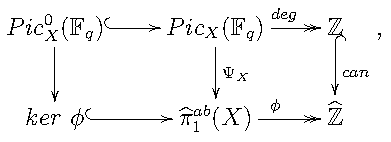
\includegraphics[width=0.3152\paperwidth]{images/L16-p134-reciprocity.pdf}\end{figure}
其中$\phi:\widehat\pi_1^{\mathrm{ab}}(X)\to\widehat{\Z}\cong\widehat\pi_1(\F_q)\cong\Gal(\overline{\F}_q/\F_q)$由结构态射$X\to\Spec\F_q$诱导，参见\eref{定理}{L10S3O2}。这里以几何Frobenius对应于$1$来识别$\Gal(\overline{\F}_q/\F_q)$与$\widehat{\Z}$。
\end{theorem}
我们已经得到以下三类对象之间的一一对应：
\begin{figure}[H]\centering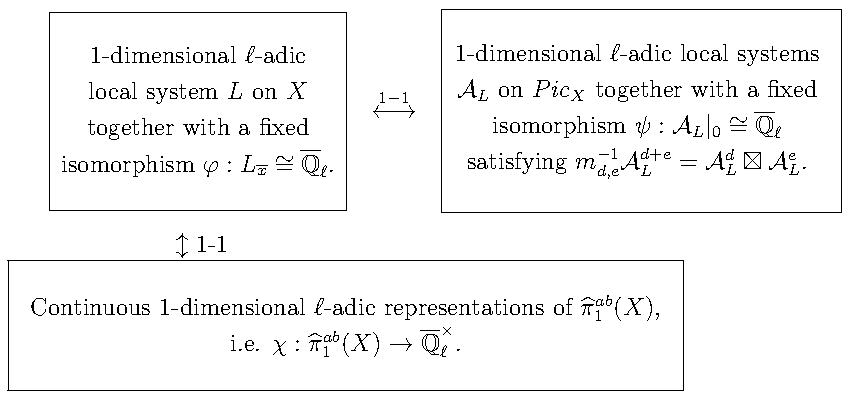
\includegraphics[width=0.6859\paperwidth]{images/L16-p134-three-correspondences.pdf}\end{figure}
为了证明\eref{定理}{L16S2O1}，需要下面的\eref{引理}{L16S2O2}和\eref{引理}{L16S2O3}，它们给出更多一一对应。设$G$为有限域$k$上的连通、分离、有限型交换群概形。
\sourcepage{135}
$G$上的\textbf{$\ell$进特征标层}$\mathcal L$\znoteplain{特征标层可以看成「群同态」的几何版本：一维 $\ell$ 进局部系统给出 $\widehat\pi_1(G)$ 的一维表示；平凡化 $\mathcal L_0\cong\overline\Q_\ell$ 固定单位元处纤维的标架，使「单位元映入 $1$」；乘法同构 $m^{-1}\mathcal L\cong\mathcal L\boxtimes\mathcal L$ 则把群乘法的相容性搬到层上。三者合起来正是「$G$ 上的乘法特征」应有的全部数据，\eref{引理}{L16S2O2}因此能把它们与 $\chi:G(k)\to\overline\Q_\ell^\times$ 一一对应起来；缺少乘法同构时只能得到一般的局部系统。（上下文推断，无外部依据）}，是一个一维$\ell$进局部系统，具有平凡化$\mathcal L_0\cong\overline{\Q}_\ell$及相容的乘法同构$m^{-1}\mathcal L\cong\mathcal L\boxtimes\mathcal L$，其中$m:G\times G\to G$为乘法。
\originalnumber{2}
\begin{lemma}\label{L16S2O2}
下列对象一一对应：
\begin{figure}[H]\centering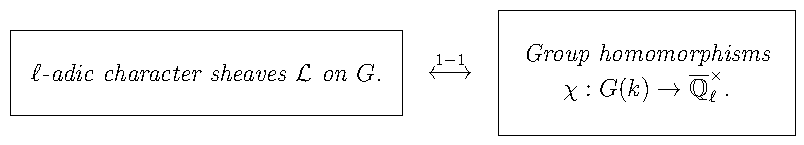
\includegraphics[width=0.6485\paperwidth]{images/L16-p135-Lang-correspondence.pdf}\end{figure}
\end{lemma}
\begin{proof}
先设$\mathcal L$为$G$上的$\ell$进特征标层。对$k$-点$x\in G(k)$，几何Frobenius在纤维$\mathcal L_x$上作用，参见\sref{L12S2}。由于$\mathcal L$为一维，该作用为$\overline{\Q}_\ell^{\times}$中的一个元素。定义
\[\chi:G(k)\longrightarrow\overline{\Q}_\ell^{\times},\qquad x\longmapsto\mathrm{Fr}_x|_{\mathcal L_x}.\]
需要证明$\chi$为群同态。由$m^{-1}\mathcal L\cong\mathcal L\boxtimes\mathcal L$，有$\mathcal L_{x+y}\cong\mathcal L_x\otimes\mathcal L_y$，所以$\chi(x+y)=\chi(x)\chi(y)$。
% [Tutor Note: 原书 p135 此处作 $\mathcal L_{\overline{x+y}}\cong\mathcal L_{\overline x}\otimes\mathcal O_{\overline y}$，其中 $\mathcal O_{\overline y}$ 显系 $\mathcal L_{\overline y}$ 之误（乘法性要求两个因子都是 $\mathcal L$ 的纤维）；译文按正确写法处理。]

反过来，设有群同态$\chi:G(k)\to\overline{\Q}_\ell^{\times}$。由于$k\cong\F_q$，可定义\textbf{Lang同源}\znoteplain{Lang 同源是有限域上特有的构造：$g\mapsto F_q(g)-g$ 把 $G(\overline k)$ 映到自身，并在几何点上成为有限平展覆盖，覆盖变换群恰为 $G(\F_q)$——这就是把「$G(\F_q)$ 的一维表示」与「$G$ 上的局部系统」接起来的桥梁。这里写加号是因为 $G$ 交换；一般群情形用 $g\mapsto F_q(g)g^{-1}$。注意 $F_q$ 是绝对 Frobenius（$g\mapsto g^q$），而不是相对的 $q^n$ 次幂，两者的覆盖变换群不同。（上下文推断，无外部依据）}
\[\varphi:G\longrightarrow G,\qquad g\longmapsto F_q(g)-g,\]
其中$F_q:G\to G$为绝对Frobenius态射$g\mapsto g^q$。Lang同源使$G$成为自身的有限平展Galois覆盖，其覆盖变换群恰为$G(\F_q)$。由平展基本群的定义，有满射$\widehat\pi_1(G)\twoheadrightarrow G(\F_q)$；由于目标交换，它经由$\widehat\pi_1^{\mathrm{ab}}(G)$分解。以几何Frobenius为约定，复合
\[\widehat\pi_1^{\mathrm{ab}}(G)\twoheadrightarrow G(\F_q)\xrightarrow{\chi^{-1}}\overline{\Q}_\ell^{\times}\]
给出一维$\ell$进局部系统$\mathcal L$。

为证明特征标层的乘法性质，只需证明$m^{-1}\mathcal L$和$\mathcal L\boxtimes\mathcal L$的基点纤维作为$\widehat\pi_1(G\times G)$表示同构。分别记两表示为$\rho_m,\rho_\boxtimes$。容易看出它们都经由$\widehat\pi_1(G\times G)\to G(\F_q)\times G(\F_q)$分解，得到下图：
\begin{figure}[H]\centering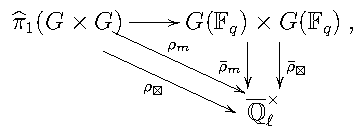
\includegraphics[width=0.2923\paperwidth]{images/L16-p135-characters.pdf}\end{figure}
\sourcepage{136}
其中$\overline\rho_m(g_1,g_2)=\chi(g_1+g_2)^{-1}$，$\overline\rho_\boxtimes(g_1,g_2)=\chi(g_1)^{-1}\chi(g_2)^{-1}$。由于$\chi$为群同态，$\rho_m=\rho_\boxtimes$。可以看出上述两个构造互为逆构造，引理得证。
% [Tutor Note: 原书 p136 此处作 $\overline\rho_m((g_1,g_2))=\chi(g_1+g_2)$、$\overline\rho_\boxtimes((g_1,g_2))=\chi(g_1)\chi(g_2)$，缺指数 $-1$；按本证明中由 $\chi^{-1}$ 构造 $\mathcal L$ 的约定，译文作 $\chi(g_1+g_2)^{-1}$ 与 $\chi(g_1)^{-1}\chi(g_2)^{-1}$。]
\end{proof}
对任意$\F_q$-有理点$x\in X$，一个\textbf{Frobenius作用}就是连续同态$\rho_x:\widehat{\Z}\cong\Gal(\overline{\F}_q/\F_q)\to\overline{\Q}_\ell^{\times}$。设$L$为$X$上的一维局部系统。由\sref{L12S2}，$\Gal(\overline{k_x}/k_x)$作用于纤维$L_{\overline x}$，给出Frobenius作用$\rho_{L,x}:\widehat{\Z}\to\GL(L_{\overline x})\cong\overline{\Q}_\ell^{\times}$。
\originalnumber{3}
\begin{lemma}\label{L16S2O3}
固定$x\in X(\F_q)$。以下两类对象的同构类一一对应：
\begin{figure}[H]\centering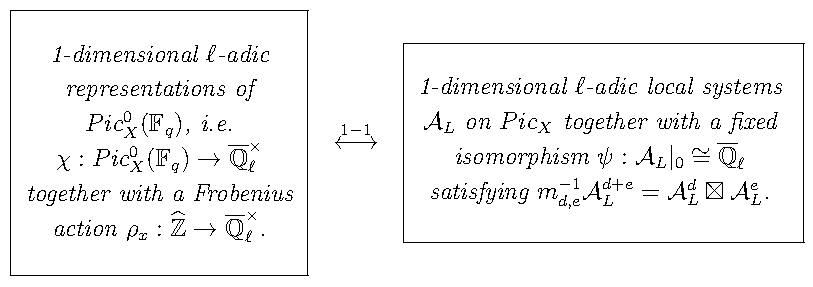
\includegraphics[width=0.6556\paperwidth]{images/L16-p136-Picard-correspondence.pdf}\end{figure}
\end{lemma}
\begin{proof}
从第二类到第一类的映射很直接：取$\mathcal A_L^0$，再应用\eref{引理}{L16S2O2}。Frobenius作用由Deligne定理从$\mathcal A_L$得到的$X$上一维局部系统$L$诱导。

反过来，有同构$m_x^d:\operatorname{Pic}_X^d\to\operatorname{Pic}_X^0$，$\mathcal E\mapsto\mathcal E(-dx)$。Frobenius作用$\rho_x$给出$\{x\}=\Spec\F_q$上的局部系统$L_x$。定义
\[\mathcal A_L^d:=(m_x^d)^{-1}\mathcal A_L^0\otimes L_x^{\otimes d},\]
便得到上述映射的逆构造。
\end{proof}
\begin{proof}[\eref{定理}{L16S2O1}的证明]
先证明下图交换：
\begin{figure}[H]\centering\begin{equation}\tag{2.1}\label{L16eq21}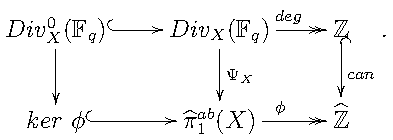
\includegraphics[width=0.3172\paperwidth]{images/L16-p136-divisors.pdf}\end{equation}\end{figure}
\sourcepage{137}
闭点$y:\Spec\F_{q^n}\to X$给出交换三角
\begin{figure}[H]\centering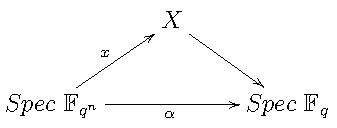
\includegraphics[width=0.2717\paperwidth]{images/L16-p137-closedpoint.pdf}\end{figure}
其中$\alpha$由包含$\F_q\hookrightarrow\F_{q^n}$诱导。因此，$\alpha$诱导的映射
\[\alpha_*:\Gal(\overline{\F}_q/\F_{q^n})\cong\widehat\pi_1(\Spec\F_{q^n})\longrightarrow\widehat\pi_1(\Spec\F_q)\cong\Gal(\overline{\F}_q/\F_q)\]
就是自然包含$\Gal(\overline{\F}_q/\F_{q^n})\hookrightarrow\Gal(\overline{\F}_q/\F_q)$。

另一方面，$\phi\circ\Psi_X(y)=\alpha_*(\mathrm{Fr}_y)$，其中$\mathrm{Fr}_y$为$\Gal(\overline{\F}_q/\F_{q^n})$的几何Frobenius生成元。容易看出，在$\Gal(\overline{\F}_q/\F_q)\cong\widehat{\Z}$的识别下，$\alpha_*(\mathrm{Fr}_y)=\deg y=n$。所以\eqref{L16eq21}中的图交换。

剩下要证明Artin映射$\Psi_X$将主除子映为单位元。正如前面所见，下列四类对象的同构类一一对应：
\begin{figure}[H]\centering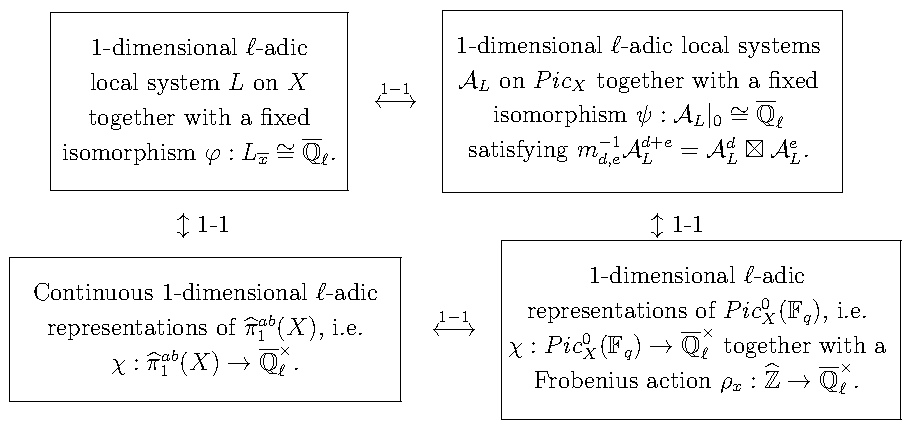
\includegraphics[width=0.7343\paperwidth]{images/L16-p137-four-correspondences.pdf}\end{figure}

由这些对应，每个一维表示$\chi_\pi:\widehat\pi_1(X)\to\overline{\Q}_\ell^{\times}$都确定同态$\chi_P:\operatorname{Pic}_X^0(\F_q)\to\overline{\Q}_\ell^{\times}$及$\rho_x:\Gal(\overline{k_x}/k_x)\to\overline{\Q}_\ell^{\times}$；这里$k_x\cong\F_q$。对任意闭点$y\in X$，我们断言
\begin{equation}\tag{2.2}\label{L16eq22}
\chi_\pi(\mathrm{Fr}[y])=\chi_P\bigl(\OO_X(y-dx)\bigr)\rho_x(\mathrm{Fr}_x)^d,\qquad d=\deg y=[k_y:\F_q].
\end{equation}
\sourcepage{138}
记$x_d$为$x$在$\F_{q^d}$上的基变换。

为证明\eqref{L16eq22}，先注意$\chi_\pi$给出$X$上的一维$\ell$进局部系统$L$。$\Gal(\overline{k_y}/k_y)$在$L_{\overline y}$上的作用诱导$\rho_y:\Gal(\overline{k_y}/k_y)\to\GL(L_{\overline y})$，得到以下交换三角：
\begin{figure}[H]\centering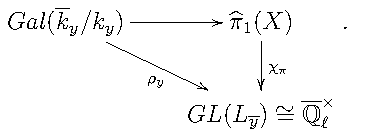
\includegraphics[width=0.2949\paperwidth]{images/L16-p138-monodromy.pdf}\end{figure}
另一方面，$\chi_P$给出$\operatorname{Pic}_X^0$上的$\ell$进特征标层$\mathcal A_L^0$。记$\widetilde y$为$y$在$\F_{q^d}$上的一个提升（即$\widetilde y:\Spec\F_{q^d}\to X$的像为闭点$y$），因而$\OO_X(\widetilde y)$为$\operatorname{Pic}_X^1$的$\F_{q^d}$-点。按\eref{引理}{L16S2O3}的构造，$\operatorname{Pic}_X^1$上的一维局部系统满足
\[\mathcal A_L^1=(m_x^1)^{-1}\mathcal A_L^0\otimes L_x.\]
由于$x_d$为位于$x$上方的$\F_{q^d}$-点，$\OO_X(\widetilde y-x_d)$为$\operatorname{Pic}_X^0$的$\F_{q^d}$-点。由Lang构造，其几何Frobenius在$\mathcal A_L^0$该纤维上的作用为
\[\chi_P\bigl(N_{\F_{q^d}/\F_q}\OO_X(\widetilde y-x_d)\bigr)=\chi_P(\OO_X(y-dx)),\]
因此，几何Frobenius在$(\mathcal A_L^1)_{\OO_X(\widetilde y)}$上的作用为$\chi_P(\OO_X(y-dx))\rho_x(\mathrm{Fr}_{x_d})$。由Deligne定理，$AJ_1^{-1}\mathcal A_L^1\cong L$，从而有交换图：
\begin{figure}[H]\centering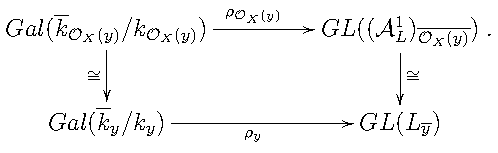
\includegraphics[width=0.4014\paperwidth]{images/L16-p138-comparison.pdf}\end{figure}
通过自然包含$\Gal(\overline{k_{x_d}}/k_{x_d})\hookrightarrow\Gal(\overline{k_x}/k_x)$，有$\mathrm{Fr}_{x_d}=(\mathrm{Fr}_x)^d$，于是得到\eqref{L16eq22}。

因此，对任意主除子$D$及$\widehat\pi_1(X)$的任意一维表示$\chi$，均有$\chi\circ\Psi_X(D)=1$。

因为$\widehat\pi_1(X)$为射有限群，对任意$1\ne s\in\widehat\pi_1(X)$，均有有限商$q_s:\widehat\pi_1(X)\to G_s$使$q_s(s)\ne1$。若$s$在$\widehat\pi_1^{\mathrm{ab}}(X)$中的像非平凡，还可取$G_s$为交换群。由有限阿贝尔群表示论的基本事实，可以找到特征标$\chi_s:G_s\to\overline{\Q}_\ell^{\times}$，使$\chi_s(q_s(s))\ne1$。复合$\chi_s\circ q_s$便是一个在$s$处非平凡的一维表示。所以，对所有主除子$D$，必有$\Psi_X(D)=1$。
\end{proof}
\sourcepage{139}
\needspace{5\baselineskip}\section{第16讲参考文献}\label{L16S3}
\begin{references}
\refitem{L16bibT}{T} Péter Tóth, \emph{Geometric abelian class field theory}, Thesis for MD at Univ. Utrecht, available at \url{http://math.bu.edu/people/magner/Seminar/GCFTthesis.pdf}.
\end{references}

\chapter{与Fourier--Mukai变换的联系}\label{L17}\lecturedate{2020/04/15}\sourcepage{140}
本讲从Fourier--Mukai变换的框架解释$\C$上$n=1$的几何Langlands对应。底域固定为$\C$，几何对象采用解析拓扑来理解；因此，局部系统指解析拓扑下局部常值的层，$\OO_X$为全纯函数层。
\section{带平坦联络的丛}\label{L17S1}\idx{平坦联络}\idx{曲率}
设$S$为$\C$上的光滑代数簇，$\mathcal E$为$S$上的全纯向量丛。以$\Omega_S^1$表示$S$上全纯微分一形式的层。$\mathcal E$上的\textbf{全纯联络}$\nabla$是一个$\C$-线性映射
\[\nabla:\mathcal E\longrightarrow\mathcal E\otimes_{\OO_S}\Omega_S^1,\]
满足$\nabla(fe)=f\nabla(e)+e\otimes df$，其中$f\in\OO_S(U)$、$e\in\mathcal E(U)$。
归纳定义$\C$-线性映射$\nabla^r:\Omega_S^r\otimes\mathcal E\to\Omega_S^{r+1}\otimes\mathcal E$如下：
\[\begin{cases}
\nabla^0=\nabla,\\
\nabla^{k+r}((a\wedge b)\otimes e)=(da\wedge b)\otimes e+(-1)^k a\wedge\nabla^r(b\otimes e),
\end{cases}\]
% [Tutor Note: 原书 p140 的展开式作 $\nabla^{k+r}((a\wedge b)\otimes e)=(da\wedge b)\otimes e+(-1)^k a\wedge\nabla^{s}(b\otimes e)$，末项上标 $s$ 未定义；按归纳定义应为 $\nabla^{r}$，译文按正确写法处理。]
其中$a\in\Omega_S^k$、$b\in\Omega_S^r$为局部截面。$\nabla$的\textbf{曲率}$R(\nabla)$为映射$\nabla^1\circ\nabla:\mathcal E\to\mathcal E\otimes\Omega_S^2$。若$R(\nabla)=0$，则称联络\textbf{平坦}或\textbf{可积}\znote{平坦联络的丛亦称带可积联络的丛：曲率 $R(\nabla)=0$ 等价于平行移动只依赖路径的同伦类，故局部水平截面给出向量丛的平凡化，转移矩阵可取常矩阵。在解析（或平展）拓扑下，这类丛与有限秩局部系统一一对应，即 Riemann--Hilbert 对应；由此其 Chern 类必为零。[来源：nLab "flat connection"，\url{https://ncatlab.org/nlab/show/flat+connection}（Last revised 2023-06-04；2026-11-14 访问）。]}。
\sourcepage{141}
对切丛$T_S$的任意局部截面$D$，有局部截面之间的映射
\[\nabla_D:\mathcal E(U)\longrightarrow\mathcal E(U),\qquad e\longmapsto\langle\nabla(e),D\rangle.\]
因而得到$\C$-线性映射$\rho_\nabla:T_S\to\mathcal End_{\C}(\mathcal E)$。以下引理可由直接计算证明。
\originalnumber{1}
\begin{lemma}\label{L17S1O1}
$\nabla$平坦，当且仅当$\rho_\nabla$为Lie代数层的同态，即局部满足
\[\nabla_{[D_1,D_2]}=\nabla_{D_1}\circ\nabla_{D_2}-\nabla_{D_2}\circ\nabla_{D_1}.\]
\end{lemma}
\originalnumber{2}
\begin{note}[L17S1O2]
若$\mathcal E$为$S$上的全纯向量丛，具有平坦联络$\nabla$，则$\nabla$诱导$\mathcal E$上的$\mathcal D_S$-模结构，并得到以下复向量空间层的复形：
% [Tutor Note: 原书 p141 此处作 "complex of sheaves of $\C$-algebras"，但该复形是复向量空间层（$\OO_S$-模层）的复形，并非 $\C$-代数层；译文按"复向量空间层"处理。]
\[\mathcal E\xrightarrow{\nabla}\mathcal E\otimes_{\OO_S}\Omega_S^1\xrightarrow{\nabla^1}\mathcal E\otimes\Omega_S^2\xrightarrow{\nabla^2}\cdots.\]
此外，$(\mathcal E,\nabla)$为完整$\mathcal D_S$模。
\end{note}
\originalnumber{3}
\begin{proposition}\label{L17S1O3}
设$\mathcal E$为带平坦联络$\nabla$的向量丛。则在足够小的局部开集上，$\nabla$的核的复维数等于$\mathcal E$的秩；水平截面层$\mathcal E^\nabla:=\ker\nabla$给出$\mathcal E$的局部平凡化，使全部转移矩阵均为常数矩阵。
\end{proposition}
\eref{命题}{L17S1O3}的证明可见\bref{L17bibP}{P}第74页。
% [Tutor Note: 原书 p141 此处作 "For a proof of Proposition 1.8"，但带平坦联络向量丛的局部平凡化是 Proposition 1.3；Proposition 1.8 是 p143 关于 $\operatorname{Pic}^\natural_A$ 的命题。同页推论 1.9 的证明中亦误引 "Proposition 1.8"，均应为 Proposition 1.3。
\originalnumber{4}
\begin{corollary}\label{L17S1O4}
在解析范畴中，带平坦联络的向量丛与有限秩复向量空间局部系统一一对应。
\end{corollary}
\begin{proof}
给定复向量空间局部系统$E$，向量丛$\mathcal E:=E\otimes_{\C}\OO_S$具有由外微分$d:\OO_S\to\Omega_S^1$给出的自然平坦联络。

反过来，对带平坦联络$\nabla$的向量丛$\mathcal E$，$\mathcal E^\nabla$为复向量空间局部系统；由\eref{命题}{L17S1O3}，$\mathcal E\cong\mathcal E^\nabla\otimes_{\C}\OO_S$。
\end{proof}
设$(\mathcal E_i,\nabla_i)$，$i=1,2$，为带联络的丛，则$\mathcal E_1\otimes\mathcal E_2$具有联络
\begin{equation}\tag{1.1}\label{L17eq11}\nabla(e_1\otimes e_2)=\nabla_1(e_1)\otimes e_2+e_1\otimes\nabla_2(e_2).\end{equation}
\begin{exercise*}\label{L17S1Ex1}
证明：若$\nabla_1$和$\nabla_2$都平坦，则\eqref{L17eq11}给出的张量积联络也平坦。提示：使用\eref{引理}{L17S1O1}。
\end{exercise*}
\sourcepage{142}
\originalnumber{5}
\begin{note}[L17S1O5]
以$\overline\Omega_S^1$表示反全纯微分一形式对应的光滑$(0,1)$-形式层。$S$上的每个全纯向量丛$\mathcal E$，都可以视为一个$C^\infty$复向量丛，带有给出全纯结构的$\C$-线性算子$\overline\partial_{\mathcal E}:\mathcal E\to\mathcal E\otimes\overline\Omega_S^1$。设$\nabla$为$\mathcal E$上的全纯联络，则$\widetilde\nabla:=\nabla+\overline\partial_{\mathcal E}$为微分几何意义下的联络，且$R(\widetilde\nabla)=R(\nabla)$。所以，具有平坦全纯联络的全纯向量丛，其有理Chern类全部为零，因为可以选取曲率矩阵为零的联络。

反过来，若$\widetilde\nabla$为$C^\infty$复向量丛$M$上的平坦联络，则其反全纯部分定义$M$上的全纯结构，全纯部分则定义一个平坦全纯联络。
\end{note}
任意两个联络$\nabla,\nabla':\mathcal E\to\mathcal E\otimes\Omega_S^1$之差都是函数线性的：
\[(\nabla-\nabla')(fe)=f(\nabla-\nabla')(e).\]
因而它是$\Hom_{\OO_S}(\mathcal E,\mathcal E\otimes_{\OO_S}\Omega_S^1)$中的元素。特别地，若$\mathcal E$为线丛，两个联络之差就是$H^0(S,\Omega_S^1)$中的元素。
\originalnumber{6}
\begin{lemma}\label{L17S1O6}
设$(\mathcal E,\nabla)$为$S$上带平坦联络的线丛。则$\mathcal E$的所有平坦联络组成以全局闭一形式空间$H^0(S,\Omega_S^1)^{\mathrm{cl}}$为平移向量空间的仿射空间。
\end{lemma}
\begin{proof}
证明是直接的。对另一个联络$\nabla'$，有$u\in H^0(S,\Omega_S^1)$使$\nabla'(e)=\nabla(e)+u\otimes e$。取$\mathcal E^\nabla$的局部基$e$，则
\[\begin{aligned}
\nabla'^1\circ\nabla'(fe)&=\nabla'^1(u\otimes fe+\nabla(fe))\\
&=\nabla'^1(fu\otimes e+df\otimes e)\\
&=d(fu)\otimes e-fu\wedge\nabla'(e)-df\wedge\nabla'(e)\\
&=d(fu)\otimes e-(fu\wedge u)\otimes e-(df\wedge u)\otimes e\\
&=du\otimes fe.
\end{aligned}\]
所以$\nabla'$平坦当且仅当$du=0$。
\end{proof}
\sourcepage{143}
\originalnumber{7}
\begin{example}\label{L17S1O7}
若$S$为曲线或阿贝尔簇\znote{阿贝尔簇指完备连通的代数群；它自动交换、射影，且群律唯一。任意 $g$ 维阿贝尔簇都形如 $V/\Lambda$（$V$ 为 $g$ 维复向量空间，$\Lambda$ 为格），故其全纯微分空间即 $V^*$。$\operatorname{Pic}^0(A)$ 是参数化与 $\OO_A$ 代数等价的线丛的连通分量，它自然同构于对偶阿贝尔簇 $A^\vee$，因此 $\dim A=\dim A^\vee$。[来源：nLab "abelian variety"，\url{https://ncatlab.org/nlab/show/abelian+variety}（Last revised 2026-09-26；2026-11-14 访问）。]}，则$H^0(S,\Omega_S^1)^{\mathrm{cl}}=H^0(S,\Omega_S^1)$。因此，在这些情形中，一旦线丛$\mathcal E$具有一个平坦联络，它的所有联络都是平坦的。
\end{example}
\originalnumber{8}
\begin{proposition}\label{L17S1O8}\idx{Picard概形的向量扩张}
设$A$为阿贝尔簇，以$\operatorname{Pic}_A^\natural$表示参数化$A$上二元组$(\mathcal E,\nabla)$的群概形，其中$\mathcal E$为线丛，$\nabla$为平坦联络；在线丛的单位点处取刚性化。自然映射$\operatorname{Pic}_A^\natural\to\operatorname{Pic}_A^0$为满射，其核为向量群$H^0(A,\Omega_A^1)$，亦即以该向量空间为平移空间的仿射空间。此外，$\operatorname{Pic}_A^\natural$为细模空间，参数化这些带平坦联络的刚性化线丛。
\end{proposition}
\eref{命题}{L17S1O8}是\bref{L17bibL}{L}中定理2.1.2的重述，证明的参考出处亦见该文。注意，$\operatorname{Pic}_A^\natural$的单位元为$(\OO_A,d)$，$(\mathcal E,\nabla)$的逆元为$(\mathcal E^\vee,\nabla^\vee)$，满足
\[\langle\nabla^\vee(e^\vee),e\rangle=-\langle e^\vee,\nabla(e)\rangle+d\langle e^\vee,e\rangle.\]
\section{用Fourier--Mukai变换解释}\label{L17S2}\idx{Fourier--Mukai变换}\idx{Poincaré线丛}
设$X$为光滑射影复曲线，其Jacobian簇为$\operatorname{Jac}(X)=\operatorname{Pic}_X^0(\C)$。这是一个阿贝尔簇。由\eref{笔记}{L15S3O2}，$X$上的秩一局部系统与$\operatorname{Jac}(X)$上的秩一局部系统一一对应。由于$\operatorname{Pic}_{\operatorname{Jac}(X)}^\natural$参数化$\operatorname{Jac}(X)$上的线丛及其全纯平坦联络，它也参数化$X$上的全部秩一局部系统。

现在令$A=\operatorname{Jac}(X)$，则$\operatorname{Pic}_A^0$为对偶阿贝尔簇$A^\vee$\znote{设复环面 $T=V/\Lambda$，$\Lambda\subset V$ 为格，其对偶环面定义为 $T^\vee=V^*/\Lambda^*$，其中 $\Lambda^*=\{\ell\in V^*:\operatorname{Im}\ell(\lambda)\in\Z,\ \forall\lambda\in\Lambda\}$。阿贝尔簇 $A$ 的对偶 $A^\vee$ 正是其作为复环面的对偶，且 $A^\vee\cong\operatorname{Pic}^0_A$；一般环面 $T$ 的代数对偶 $\operatorname{Hom}(X^*(T),\C^*)$ 满足 $X^*(T^\vee)=X_*(T)$，是 Cartier 对偶的特例。两个环面互为对偶，且 $(T^\vee)^\vee=T$；阿贝尔簇与其对偶之间的 Fourier--Mukai 变换，正是这种对偶在层论层面的体现。[来源：nLab "Cartier duality"，\url{https://ncatlab.org/nlab/show/Cartier+duality}（Last revised 2025-10-19；2026-11-14 访问）。]}，$A\times A^\vee$上有Poincaré线丛$\mathcal P$。曲线的Jacobian簇具有主极化\znote{阿贝尔簇 $A$ 的极化指由丰沛线丛 $\mathcal L$ 给出的同源 $\varphi_{\mathcal L}:A\to A^\vee$，$x\mapsto t_x^*\mathcal L\otimes\mathcal L^{-1}$；若 $\varphi_{\mathcal L}$ 为同构，则称 $\mathcal L$（或该极化）为\textbf{主极化}。曲线 $X$ 的 Jacobian 上，由 $X\to\operatorname{Jac}(X)$ 拉回构造的 theta 线丛给出主极化，故 $\operatorname{Jac}(X)\cong\operatorname{Jac}(X)^\vee$，这正是下文可取 $\theta$ 使 (2.1) 成为同构的原因。极化还固定了丰沛线丛的代数等价类，因而是主极化阿贝尔簇的模空间理论中的基本不变量。[来源：MathWorld 词条「Abelian Variety Polarization」，\url{https://mathworld.wolfram.com/AbelianVarietyPolarization.html}（2026-11-14 访问）。]}，因此可以在$A$上选取给出主极化的线丛$\theta$，定义同构
\begin{equation}\tag{2.1}\label{L17eq21}\Phi_\theta:A\xrightarrow{\sim}A^\vee,\qquad x\longmapsto t_x^*\theta\otimes\theta^{-1}.\end{equation}
由\eref{命题}{L17S1O8}，有正合列
\[0\longrightarrow H^0(A,\Omega_A^1)\longrightarrow\operatorname{Pic}_A^\natural\xrightarrow{p}A^\vee\longrightarrow0.\]
\sourcepage{144}
另一方面，通过上述局部系统对应，$\operatorname{Pic}_A^\natural$也参数化$X$上的线丛$L$及其平坦联络$\delta$，于是有映射$q:\operatorname{Pic}_A^\natural\to A=\operatorname{Jac}(X)$，$(L,\delta)\mapsto L$。我们将看到，适当选取$\theta$后，下列三角交换：
\begin{figure}[H]\centering\begin{equation}\tag{2.2}\label{L17eq22}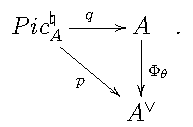
\includegraphics[width=0.1553\paperwidth]{images/L17-p144-polarization.pdf}\end{equation}\end{figure}
通过$p\times\mathrm{id}_A$，将Poincaré线丛拉回到$\operatorname{Pic}_A^\natural\times A$，得到线丛$\widetilde{\mathcal P}$及其万有相对平坦联络
\[\widetilde\nabla:\widetilde{\mathcal P}\longrightarrow\operatorname{pr}_A^*\Omega_A^1\otimes\widetilde{\mathcal P},\]
其中$\operatorname{pr}_A$、$\operatorname{pr}_\natural$分别为到$A$、到$\operatorname{Pic}_A^\natural$的投影。
在代数凝聚范畴中，定义Fourier--Mukai变换\znote{给定概形 $X,Y$ 与核 $K\in D^b_{\mathrm{coh}}(X\times Y)$，Fourier--Mukai 变换为 $\Phi_K(E)=\mathrm Rq_*(p^*E\overset{\mathrm L}{\otimes}K)$，其中 $p,q$ 为 $X\times Y$ 到 $X,Y$ 的投影。它是 Radon 变换在导出范畴中的公理化版本：核可取结构层、Poincaré 线丛等。Mukai 以 $K=\mathcal P$ 证明了 $D^b(X)\cong D^b(X^\vee)$，这正是一维几何 Langlands 对应的原型。当 $X,Y$ 为阿贝尔簇、核取 Poincaré 线丛时，$\Phi_K$ 是导出范畴的等价，即 Mukai 对偶；核的一般选取只使 $\Phi_K$ 成为函子。[来源：nLab "Fourier-Mukai transform"，\url{https://ncatlab.org/nlab/show/Fourier-Mukai+transform}（Last revised 2025-10-21；2026-11-14 访问）。]}$\mathfrak F_A$和$\mathfrak F_\natural$如下：
\[\mathfrak F_A:D_{\mathrm{coh}}^b(\mathcal D_A)\longrightarrow D_{\mathrm{coh}}^b(\OO_{\operatorname{Pic}_A^\natural}),\]
\[\mathfrak F_A(\mathcal K^\bullet):=\mathrm R(\operatorname{pr}_\natural)_*\operatorname{DR}_{\operatorname{Pic}_A^\natural\times A/\operatorname{Pic}_A^\natural}\bigl((\widetilde{\mathcal P},\widetilde\nabla)\overset{\mathrm L}{\otimes}\operatorname{pr}_A^*\mathcal K^\bullet\bigr).\]
这里，对光滑满射$Y\to S$，$\operatorname{DR}_{Y/S}$为相对de Rham复形，参见\lref{L14}，定义为
\[\operatorname{DR}_{Y/S}(\mathcal F^\bullet):=\omega_{Y/S}\overset{\mathrm L}{\otimes}_{\mathcal D_{Y/S}}\mathcal F^\bullet,\]
另一个变换为
\[\mathfrak F_\natural:D_{\mathrm{coh}}^b(\OO_{\operatorname{Pic}_A^\natural})\longrightarrow D_{\mathrm{coh}}^b(\mathcal D_A),\]
\[\mathfrak F_\natural(\mathcal K^\bullet):=\mathrm R(\operatorname{pr}_A)_*\bigl((\widetilde{\mathcal P},\widetilde\nabla)\overset{\mathrm L}{\otimes}_{\OO_{\operatorname{Pic}_A^\natural\times A}}\operatorname{pr}_\natural^*\mathcal K^\bullet\bigr).\]
\originalnumber{1}
\begin{theorem}\label{L17S2O1}
有以下典范的函子同构：
\[\begin{aligned}
\mathfrak F_\natural\circ\mathfrak F_A&\cong(-1)_A^*(\cdot)[-g(X)]&&\text{在 }D_{\mathrm{coh}}^b(\mathcal D_A)\text{上},\\
\mathfrak F_A\circ\mathfrak F_\natural&\cong(-1)_{\operatorname{Pic}_A^\natural}^*(\cdot)[-g(X)]&&\text{在 }D_{\mathrm{coh}}^b(\OO_{\operatorname{Pic}_A^\natural})\text{上}.
\end{aligned}\]
其中，对群概形$G$，$(-1)_G:G\to G$为将每个元素送到其逆元的态射。
\end{theorem}
\sourcepage{145}
现在取支撑于$p\in\operatorname{Pic}_A^\natural$的摩天层\znote{对闭点 $p\in S$，以 $p$ 为支撑的\textbf{摩天层}是 $i_{p*}\C$（其 $\OO_S$-模版本记为 $\OO_p$），其中 $i_p:\{p\}\hookrightarrow S$ 为嵌入；它在 $p$ 以外的茎全为零，在 $p$ 处的茎为 $\C$。摩天层是凝聚层导出范畴的一组紧生成元，其 Fourier--Mukai 像给出 $\mathcal D$-模，因而成为几何 Langlands 对应的基本构件。由于它只有一个非零茎，$\OO_p$ 还是 $\mathcal D$-模一侧最小、最易计算的构件。[来源：nLab "skyscraper sheaf"，\url{https://ncatlab.org/nlab/show/skyscraper+sheaf}（Last revised 2016-06-23；2026-11-14 访问）。]}$\OO_p$；$p=(L,\delta)$通过上述对应表示$X$上的线丛及其平坦联络。则
\[\mathfrak F_\natural(\OO_p)=\bigl(\widetilde{\mathcal P}|_{\{p\}\times A},\widetilde\nabla|_{\{p\}\times A}\bigr)\]
为$\mathcal D_A$模，恰是在几何Langlands对应下与$(L,\delta)$相对应的对象。从这一角度看，Langlands对应是Fourier--Mukai变换的一个特殊情形。此外，摩天层是有限支撑凝聚层的一族基本构件；相应的Hecke特征层可以看作这一子范畴的Fourier--Mukai像的基本构件。\idx{摩天层}
\section{\texorpdfstring{$\operatorname{Jac}(X)$上的行列式线丛}{Jac(X)上的行列式线丛}}\label{L17S3}\idx{行列式线丛}\idx{主极化}
我们要找到适当的线丛$\theta$，使\eqref{L17eq22}的三角交换。

设$\alpha:X\to B$为从曲线到阿贝尔簇的非常值态射，$B^\vee$为对偶阿贝尔簇，$\mathcal P_B$为$B^\vee\times B$上的Poincaré线丛。对$X$上的凝聚层$\mathcal F$，考虑其Fourier变换
\[\mathfrak F_{B^\vee}(\mathcal F):=\mathrm R(\operatorname{pr}_{B^\vee})_*\bigl(\operatorname{pr}_B^*\mathrm R\alpha_*\mathcal F\overset{\mathrm L}{\otimes}\mathcal P_B\bigr),\]
并将它视为$B^\vee$上凝聚层的Grothendieck群$K(B^\vee)$中的元素。该元素实际上属于由局部自由层生成的子群$K^0(B^\vee)$，因而可以定义与$\mathcal F$相关的行列式线丛$S(\mathcal F):=\det(\mathfrak F_{B^\vee}(\mathcal F))$。

映射$\mathcal F\mapsto S(\mathcal F)$给出从$X$上凝聚层的Grothendieck群$K(X)$到$\operatorname{Pic}_{B^\vee}$的群同态。特别地，
\[\begin{aligned}
S\bigl(\OO_X(\textstyle\sum_i n_ip_i)\bigr)&\cong S(\OO_X)\otimes\bigotimes_iS(\OO_{p_i})^{\otimes n_i}\\
&\cong S(\OO_X)\otimes\bigotimes_i(\mathcal P_B|_{\alpha(p_i)})^{\otimes n_i}.
\end{aligned}\]
因此得到映射
\[\operatorname{Div}(X)\longrightarrow\operatorname{Pic}_{B^\vee}^0\cong B,\qquad\sum_i n_ip_i\longmapsto\bigotimes_i(\mathcal P_B|_{\alpha(p_i)})^{\otimes n_i}.\]
它经由$\operatorname{Div}(X)\to\operatorname{Pic}_X$分解，故给出$\alpha_*:\operatorname{Pic}_X\to\operatorname{Pic}_{B^\vee}^0\cong B$。
\originalnumber{1}
\begin{proposition}\label{L17S3O1}
设$L$为$X$上的线丛。由行列式线丛的逆$S(L)^{-1}\in\operatorname{Pic}_{B^\vee}$按\eqref{L17eq21}诱导的映射$\Phi_{S(L)^{-1}}:B^\vee\to B$，等于复合
\[B^\vee\cong\operatorname{Pic}_B^0\xrightarrow{\alpha^*}\operatorname{Pic}_X^0\xrightarrow{\alpha_*}\operatorname{Pic}_{B^\vee}^0\cong B.\]
\end{proposition}
% [Tutor Note: 原书 p145 的命题 3.1 作 $\Phi_{S(L)}:B^\vee\to B$，由行列式线丛 $S(L)\in\operatorname{Pic}_{B^\vee}$ 诱导；译文按 $\Phi_{S(L)^{-1}}$ 处理，以与本节下文 $\Phi_{S(L)^{-1}}=\alpha_*$ 的复合方向一致。]
\sourcepage{146}
现在令$B=A^\vee$，其中$A=\operatorname{Jac}(X)$。固定$p_0\in X$，则$X\times A$上有唯一的归一化Poincaré线丛$\mathcal P_X$，满足$\mathcal P_X|_{\{p_0\}\times A}\cong\OO_A$。族$\mathcal P_X$诱导分类映射$\alpha:X\to B$。由于$\mathcal P_X\cong(\alpha\times\mathrm{id}_A)^*\mathcal P_B$，映射$\alpha^*:\operatorname{Pic}_B^0\to\operatorname{Pic}_X^0$在$A\cong\operatorname{Pic}_B^0\cong\operatorname{Pic}_X^0$的识别下是恒等映射。因此，由\eref{命题}{L17S3O1}，$\Phi_{S(L)^{-1}}=\alpha_*$。

另一方面，若$g(X)\ge1$，有嵌入
\begin{equation}\tag{3.1}\label{L17eq31}i:X\hookrightarrow A,\qquad p\longmapsto\OO_X(p-p_0).\end{equation}
容易看出$i_*:\operatorname{Pic}_X^0\to A$为恒等映射，而$i^*$为$\alpha_*$的逆。以$S_A(L_0)$表示通过映射$i:X\to A$得到的通常Fourier变换$F_A(L_0)\in K(A)$的行列式线丛。由Deligne关于阿贝尔Langlands对应的几何证明，有：
\originalnumber{2}
\begin{proposition}\label{L17S3O2}
对$X$上的任意线丛$L_0$，令$\theta:=S_A(L_0)\in\operatorname{Pic}_A$，$\theta':=S(L_0)\in\operatorname{Pic}_{A^\vee}$。则下列三角交换，且$\Phi_{\theta'}$为$\Phi_\theta$的逆同构\znoteplain{（上下文推断，无外部依据）本讲的 $\theta$ 与经典 theta 除子 $\OO(\Theta)$ 相差一个逆：经典叙述里 $\OO(\Theta)$ 丰沛、$\Theta=\{L:H^0(L\otimes L_0)\ne0\}$，而注记 3.3 说 $\theta^{-1}$ 丰沛且有在 $\{L:H^0(L\otimes L_0)\ne0\}$ 上消失的截面，两者正好互为逆。故命题 3.2 的三角与注记 3.3 的丰沛方向均以原书为准，读文献时需按各自约定换算。}：
\begin{figure}[H]\centering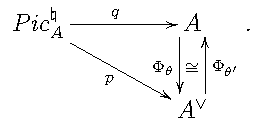
\includegraphics[width=0.2196\paperwidth]{images/L17-p146-dualpolarization.pdf}\end{figure}
\end{proposition}
% [Tutor Note: 原书 p146 的命题 3.2 作 $\theta'=S(L_0)\in\operatorname{Pic}_B$、$\theta=S_A(L_0)\in\operatorname{Pic}_A$（其中 $B=A^\vee$），而注记 3.3 又作 $\theta^{-1}$ 为丰沛线丛。原书未定义 $S(L_0)$、$S_A(L_0)$ 中取逆的约定，属约定不明而非笔误；译文照原文直译（$\theta=S_A(L_0)$、$\theta'=S(L_0)$），见命题 3.2 后的译者按。]
\begin{proof}
设$(L,\delta)$为$X$上带平坦联络的线丛。由Langlands对应，在$\operatorname{Pic}_X$上有带平坦联络的线丛$(\mathcal E,\nabla)$，满足$L\cong i^*\mathcal E$，其中$i$由\eqref{L17eq31}定义。
\end{proof}
\originalnumber{3}
\begin{note}[L17S3O3]
若$L_0$的次数为$g(X)-1$，则$\theta^{-1}=S_A(L_0)^{-1}$为丰沛线丛，并具有一个在相差非零常数倍的意义下唯一的截面。该截面恰好在满足$H^0(X,L\otimes L_0)\ne0$的点$L\in\operatorname{Pic}_X^0$处消失。
% [Tutor Note: 原书 p146 的注记 3.3 作 "$\theta^{-1}$ is an ample line bundle"；按命题 3.2 的直译 $\theta=S_A(L_0)\in\operatorname{Pic}_A$，此处即 $\theta^{-1}=S_A(L_0)^{-1}$。原书对取逆约定不明，译文照原文处理，见命题 3.2 后的译者按。]
\end{note}
\needspace{5\baselineskip}\section{第17讲参考文献}\label{L17S4}
\begin{references}
\refitem{L17bibL}{L} G. Laumon, \emph{Transformation de Fourier généralisée}, arXiv e-prints: \href{https://arxiv.org/abs/alg-geom/9603004}{alg-geom/9603004}.
\refitem{L17bibR}{R} M. Rothstein, \emph{Connections on the total Picard sheaf and the KP hierarchy}, Acta Applicandae Mathematicae 42 (1996) 297--308.
\sourcepage{147}
\end{references}
\needspace{4\baselineskip}关于平坦联络的命题：
\begin{references}
\refitem{L17bibP}{P} F. Pham, \emph{Singularités des systèmes différential de Gauss-Manin}, Progr. in Math. 2, Birkhäuser Verlag (1979).
\end{references}

\chapter{其他约化群的Langlands对应I：根数据与约化群}\label{L18}\lecturedate{2020/04/20}\sourcepage{148}
我们希望对约化群表述一个与Langlands对应中的相容性结论类似的命题。
\section{根数据与根系}\label{L18S1}\idx{根数据}\idx{根系}\idx{余根}\idx{Weyl群}
\begin{definition*}
\textbf{根数据}是一个四元组$\Psi=(X,\Phi,X^\vee,\Phi^\vee)$，其中$X,X^\vee$为有限秩自由阿贝尔群，并通过完美配对$\langle\ ,\ \rangle:X\times X^\vee\to\Z$互为对偶；$\Phi\subseteq X$、$\Phi^\vee\subseteq X^\vee$为有限子集，具有双射$\alpha\mapsto\alpha^\vee$\znote{根数据是约化群与其根系之间不依赖基的最小资料：$X$ 是极大环面的特征标格，$X^\vee$ 是余特征标格，$\Phi$ 与 $\Phi^\vee$ 为根与余根，由 $\alpha\mapsto\alpha^\vee$ 配对。它比根系多带了「环面部分」，因而能区分 $\SL_n$ 与 $\\operatorname{PGL}_n$ 这类根系相同而中心不同的群；对偶 $\Psi^\vee$ 交换 $X$ 与 $X^\vee$，正是 Langlands 对偶的来源。[来源：T.A. Springer, \textit{Reductive groups}, in \textit{Automorphic forms, representations and L-functions}, Proc. Symp. Pure Math. 33, Part 1, AMS 1979, pp.~3--27（本讲参考文献 [S]）。]}。还要求满足以下两条公理：
\begin{description}
\item[(RD1)] 对任意$\alpha\in\Phi$，$\langle\alpha,\alpha^\vee\rangle=2$。
\item[(RD2)] 对任意$\alpha\in\Phi$，$s_\alpha(\Phi)\subseteq\Phi$、$s_{\alpha^\vee}(\Phi^\vee)\subseteq\Phi^\vee$，其中$s_\alpha$、$s_{\alpha^\vee}$分别为$X$、$X^\vee$的自同态，定义为
\begin{equation}\tag{1.1}\label{L18eq11}s_\alpha(x)=x-\langle x,\alpha^\vee\rangle\alpha,\qquad s_{\alpha^\vee}(u)=u-\langle\alpha,u\rangle\alpha^\vee.\end{equation}
\end{description}
\end{definition*}
显然，若$\Psi=(X,\Phi,X^\vee,\Phi^\vee)$为根数据，则$\Psi^\vee=(X^\vee,\Phi^\vee,X,\Phi)$也是根数据，称为$\Psi$的\textbf{对偶}。

设$\Psi$为根数据，$Q$为$\Phi$生成的$X$的子群，令$V=Q\otimes_{\Z}\Q$。类似地定义$X^\vee$的子群$Q^\vee$及向量空间$V^\vee$。若$(Q^\vee)^\perp=\{0\}$，称$\Psi$\textbf{半单}；若$\Phi$为空，称它为\textbf{环面型}。
% [Tutor Note: 原书 p148 作 $V=Q\otimes\Q$，漏了下标 $\Z$；$Q$ 是自由阿贝尔群，其有理化应为 $V=Q\otimes_{\Z}\Q$，译文已补。]
\sourcepage{149}
假设$\Phi\ne\varnothing$。$V^\vee$可识别为$V$的对偶向量空间，仍以$\langle\ ,\ \rangle$表示配对。于是$\Phi$为$V$中的根系\znote{根系是根数据忘掉 $X,X^\vee$ 之后剩下的反射群资料：$V$ 为根张成的有理向量空间，三条公理要求每个根有唯一余根、反射 $s_\alpha$ 保持 $\Phi$、且 $\alpha^\vee$ 在 $\Phi$ 上取整值。由根数据构造时 $\Phi$ 自动张成 $V$。从根数据到根系要丢掉 $X,X^\vee$ 中与根无关的环面部分，故根系比根数据粗；Langlands 对偶必须用根数据而不能只用根系，这也是教材先讲根系、再讲根数据的原因。[来源：T.A. Springer, \textit{Reductive groups}, in \textit{Automorphic forms, representations and L-functions}, Proc. Symp. Pure Math. 33, Part 1, AMS 1979, pp.~3--27（本讲参考文献 [S]）。]}，意义如下。
\begin{definition*}
$V$中的\textbf{根系}$\Phi$满足：
\begin{description}
\item[(RS1)] $\Phi$有限、张成$V$，且$0\notin\Phi$。
\item[(RS2)] 对每个$\alpha\in\Phi$，存在$\alpha^\vee\in V^\vee$，满足$\langle\alpha,\alpha^\vee\rangle=2$，并且\eqref{L18eq11}定义的$s_\alpha$保持$\Phi$。
\item[(RS3)] 对每个$\alpha\in\Phi$，$\alpha^\vee(\Phi)\subseteq\Z$。
\end{description}
\end{definition*}
反射$s_\alpha$生成$\GL(V)$的一个子群，称为$\Phi$的\textbf{Weyl群}，记为$W(\Phi)$。由(RS1)、(RS2)，$W(\Phi)$可嵌入$\operatorname{Aut}(\Phi)$；$\Phi$为有限集，故$\operatorname{Aut}(\Phi)$及$W(\Phi)$都有限。

设$\Phi\subseteq V$为根系，令$V_{\R}:=V\otimes_{\Q}\R$。若超平面$H\subseteq V_{\R}$是某个$\alpha^\vee\in\Phi^\vee$的核，即与该余根正交，则称$H$为\textbf{奇异超平面}。\textbf{Weyl室}$C$是全部奇异超平面之并的补集的一个连通分支。每个Weyl室确定根的一个正负划分：$\alpha>0$当且仅当对所有$x\in C$，$\langle x,\alpha^\vee\rangle>0$。\idx{Weyl室}\idx{单根}
% [Tutor Note: 原书 p149 作 $V_R:=V\otimes_{\Q}\C$，并说 Weyl 室 $C$ 是 $V_\C$ 的子集；奇异超平面是实超平面，「连通分支」只在实向量空间中有意义，故应为 $V_\R:=V\otimes_{\Q}\R$，译文按 $\R$ 处理。]

对于所选的正负划分，若根$\alpha$为正根，且不能表示为两个正根之和，则称它为\textbf{单根}。单根集合$\Delta$称为$\Phi$的\textbf{基}。有以下性质。
\begin{enumerate}[label=\arabic*.]
\item $W(\Phi)$在Weyl室集合上单传递作用。
\item $s_\alpha$，$\alpha\in\Delta$，生成$W(\Phi)$；更确切地说，$(W,(s_\alpha)_{\alpha\in\Delta})$为Coxeter系统。
\item 每个根都是单根的整系数线性组合，其非零系数具有相同符号。因此$\Phi=\Phi^+\sqcup\Phi^-$。
\end{enumerate}
若根系不是两个非零子根系的直和，则称其\textbf{不可约}。若基$\Delta$不能分解为两个非空不交子集$\Delta'\sqcup\Delta''$，使$(\Delta'+\Delta'')\cap\Phi=\varnothing$，则称$\Delta$\textbf{连通}。有：$\Phi$不可约当且仅当$\Delta$连通。

若对每个$\alpha\in\Phi$，$\Phi$中与$\alpha$成比例的根只有$\pm\alpha$，则称$\Phi$\textbf{约化}。
\sourcepage{150}
\textbf{带基根数据}是六元组$\Psi_0=(X,\Phi,\Delta,X^\vee,\Phi^\vee,\Delta^\vee)$，其中$(X,\Phi,X^\vee,\Phi^\vee)$为根数据，$\Phi$约化，$\Delta$为$\Phi$的一组基。带基根系由Dynkin图分类，其中不可约根系对应连通Dynkin图。
\section{约化群}\label{L18S2}\idx{幺幂群}\idx{根基}\idx{Borel子群}
设$k$为域，除非另有说明，假设$k$代数闭。本节的约化群默认连通。\textbf{线性代数$k$群}$G$是具有群结构的仿射簇，且全部群运算为正则映射。特别地，乘法和求逆由代数簇态射$\mu:G\times G\to G$、$\rho:G\to G$给出，等价地由$k$-代数同态
\[\mu^\natural:k[G]\to k[G]\otimes_k k[G],\qquad\rho^\natural:k[G]\to k[G]\]
给出。每个$k$群$G$都有相应Lie代数$\g$，$G$在$\g$上有自然的伴随作用。

连通$k$群$G$\textbf{可解}，当且仅当存在群嵌入$G\hookrightarrow\GL_n(k)$使其像包含于上三角矩阵群。
% [Tutor Note: 原书 p150 作 $G\hookrightarrow\GL(k)$，漏了下标 $n$；按上下文应为 $G\hookrightarrow\GL_n(k)$，译文已补。]$G$\textbf{幺幂}，当且仅当可将其嵌入对角元全为$1$的上三角矩阵群。$G$的最大连通正规可解子群称为\textbf{根基}，记为$R(G)$。事实上，
\[R(G)=\Bigl(\bigcap_{B\subseteq G\text{为Borel子群}}B\Bigr)^0.\]
$G$的最大连通正规幺幂子群称为\textbf{幺幂根基}，记为$R_u(G)$。
\originalnumber{1}
\begin{definition}\label{L18S2O1}
\begin{enumerate}[label=(\arabic*)]
\item 若$R(G)$为环面，等价地，若$R_u(G)$平凡，则称$G$\textbf{约化}\znote{约化即「根基是环面」或等价地「幺幂根基平凡」，直观上是从 $G$ 中剥掉幺幂部分后剩下的群；$\GL_n$、$\SL_n$、$\SO_n$、$\\operatorname{Sp}_{2n}$ 都是约化群。约化比半单多一个中心环面因子，特征零时约化群的 Lie 代数约化（伴随表示完全可约）。易错点：约化（reductive）不等于线性约化（linearly reductive，指表示完全可约）；特征 $p>0$ 时 $\GL_p$ 约化却非线性约化。[来源：T.A. Springer, \textit{Reductive groups}, in \textit{Automorphic forms, representations and L-functions}, Proc. Symp. Pure Math. 33, Part 1, AMS 1979, pp.~3--27（本讲参考文献 [S]）。]}。
\item 若连通$k$群$G$的$R(G)$平凡，则称$G$\textbf{半单}。在特征零时，这等价于其Lie代数$\g$半单。
\end{enumerate}
\end{definition}
在代数闭的特征零域上，半单Lie代数与约化根系的同构类一一对应。设$G$为连通约化$k$群。对任意子环面$S\subseteq G$，将$S$在$\g$上的伴随表示对角化，出现的非平凡特征标集合记为$\Phi(G,S)$。
\sourcepage{151}

\originalnumber{2}
\begin{example}\label{L18S2O2}
令$G=\SL_2(\C)$，$S=\{\operatorname{diag}(a,b)\mid ab=1\}$。选取$\g$的基
\[e=\begin{pmatrix}0&1\\0&0\end{pmatrix},\quad f=\begin{pmatrix}0&0\\1&0\end{pmatrix},\quad h=\begin{pmatrix}1&0\\0&-1\end{pmatrix}.\]
在此基下，伴随表示为
\[\rho:S\longrightarrow\GL(\g)\cong\GL_3(\C),\qquad\operatorname{diag}(a,b)\longmapsto\operatorname{diag}(ab^{-1},a^{-1}b,1).\]
% [Tutor Note: 原书 p151 在此基 $(e,f,h)$ 下把矩阵写作 $\operatorname{diag}(a^{-1}b,ab^{-1},1)$；但 $e=E_{12}$ 的重量为 $ab^{-1}$、$f=E_{21}$ 的重量为 $a^{-1}b$（见同一页 $\chi_\pm=(a^{-1}b)^{\pm1}$ 的指标约定），故按所列基序应为 $\operatorname{diag}(ab^{-1},a^{-1}b,1)$，译文按后者处理。]
因此$(e,f,h)$将$S$的伴随表示对角化。此外，$\Phi(G,S)=\{\chi_+,\chi_-\}$，其中$\chi_\pm(\operatorname{diag}(a,b))=(ab^{-1})^{\pm1}$。
\end{example}
固定$G$的极大环面$T$\znote{极大环面是 $G$ 中维数最大的环面子群。代数闭域上所有极大环面彼此共轭，且共轭可由 Weyl 群实现，故根数据 $\Psi(G,T)$ 不依赖 $T$ 的选取。$\GL_n$ 的对角环面、$\SO_n$ 的旋转环面都是极大环面。分裂约化群正是「存在定义于 $k$ 且在 $k$ 上分裂的极大环面」的群，因此其根数据可直接用 $X^*(T)$ 描述。[来源：nLab "maximal torus"，\url{https://ncatlab.org/nlab/show/maximal+torus}（Last revised 2026-04-28；2026-11-14 访问）。]}。对应于$(G,T)$的根数据为$\Psi(G,T)=(X,\Phi,X^\vee,\Phi^\vee)$。这里$X=X^*(T)$为$T$的代数特征标群，$X^\vee=X_*(T)$为$T$的一参数乘法子群，即余特征标群。配对定义为
\[\langle x,u\rangle\in\Z,\qquad x(u(t))=t^{\langle x,u\rangle},\quad u:\mathbb G_m\to T,\ x:T\to\mathbb G_m.\]
根系$\Phi$为$\Phi(G,T)$。接下来描述$\Phi^\vee$。对$\alpha\in\Phi(G,T)$，令$T_\alpha$为$\ker\alpha$的单位连通分支。$T_\alpha$在$G$中的中心化子$Z_\alpha$为连通约化群，具有极大环面$T$；其导出群$G_\alpha:=[Z_\alpha,Z_\alpha]$为秩一半单群。实际上，$T$在$\g$上的伴随作用给出分解
\begin{equation}\tag{2.1}\label{L18eq21}\g=\mathfrak t\oplus\bigoplus_{\beta\in\Phi}\g_\beta,\end{equation}
其中$\mathfrak t=\operatorname{Lie}(T)$，且$\dim_k\g_\beta=1$。$Z_\alpha$的Lie代数为$\mathfrak t\oplus\g_\alpha\oplus\g_{-\alpha}$，$T_\alpha$以有限核映到$Z_\alpha/G_\alpha$。
% [Tutor Note: 原书 p151 作「$T_\alpha$ maps identically to its image in $Z_\alpha/G_\alpha$」；实际 $\ker(T_\alpha\to Z_\alpha/G_\alpha)=T_\alpha\cap G_\alpha\subset\mu_2$ 有限，同态并非同构，译文按「以有限核」处理。]$G_\alpha$包含一维环面；在特征零时，$\operatorname{Lie}(G_\alpha)\cong\mathfrak{sl}_2(k)=kh\oplus ke\oplus kf$，其中$h,e,f$如\eref{例题}{L18S2O2}。
\sourcepage{152}
存在唯一的余根同态$\alpha^\vee:\mathbb G_m\to G_\alpha$，其像位于$T$中，并满足$\langle\alpha,\alpha^\vee\rangle=2$。乘法映射$\operatorname{Im}(\alpha^\vee)\times T_\alpha\to T$为同源。在上述特征零的Lie代数识别下，$\alpha^\vee$的像的Lie代数为$kh$。
% [Tutor Note: 原书 p152 作 $T=(\operatorname{Im}\alpha^\vee)\times T_\alpha$ 且 $\langle\alpha,\alpha^\vee\rangle$ 后缺 $=2$；乘法映射 $\operatorname{Im}(\alpha^\vee)\times T_\alpha\to T$ 只在交为 $\operatorname{Im}\alpha^\vee\cap T_\alpha$（有限）的意义下是同源，译文按此处理。]
\originalnumber{3}
\begin{example}\label{L18S2O3}
令$G=\SL_2(\C)$，$T=\{\operatorname{diag}(a,b)\mid ab=1\}$。已经看到$\Phi(G,T)=\{\chi_+,\chi_-\}$，$\chi_\pm(\operatorname{diag}(a,b))=(ab^{-1})^{\pm1}$。所有特征标可写为$\chi_{(n,m)}(\operatorname{diag}(a,b))=a^nb^m$；由于$ab=1$，有
\[X^*(T)\cong\Z^2/\Z(1,1)\cong\Z.\]
% [Tutor Note: 原书 p152 例 2.3 作 $X\cong\Z^2$，漏了关系 $ab=1$；正确为 $X^*(T)\cong\Z^2/\Z(1,1)\cong\Z$，译文已补。]
$T_{\chi_\pm}$平凡，相应余根为
\[\chi_\pm^\vee(t)=\operatorname{diag}(t^{\pm1},t^{\mp1}).\]
\end{example}
有以下定理。
\originalnumber{4}
\begin{theorem}\label{L18S2O4}
设$k$代数闭。对任意根系约化的根数据$\Psi$，都存在连通约化群$G$及其极大环面$T\subseteq G$，满足$\Psi=\Psi(G,T)$。$(G,T)$在相差同构的意义下唯一。
\end{theorem}
我们已经说明如何从约化群得到根数据。反过来，给定根数据$\Psi=(X,\Phi,X^\vee,\Phi^\vee)$，希望构造约化群$G_\Psi$。以下给出特征零下的一种构造。先选取单根集$\Delta$，考虑范畴$C(\Psi)$，其对象和态射如下。
\begin{enumerate}[label=(\arabic*)]
\item 对象为有限维$k$向量空间族$(V_\mu)_{\mu\in X}$，以及对$\mu\in X$、$\alpha\in\Delta$给出的算子$e_\alpha:V_\mu\to V_{\mu+\alpha}$、$f_\alpha:V_\mu\to V_{\mu-\alpha}$，满足：
\begin{enumerate}[label=(\alph*)]
\item $\{\mu\mid V_\mu\ne0\}$为有限集；
\item $[e_\alpha,f_\beta]|_{V_\mu}=\delta_{\alpha\beta}\langle\mu,\alpha^\vee\rangle\mathrm{Id}_{V_\mu}$，其中
\[[e_\alpha,f_\beta]=e_\alpha f_\beta-f_\beta e_\alpha:V_\mu\to V_{\mu+\alpha-\beta}.\]
% [Tutor Note: 原书 p152 (1)(b) 把 $[e_\alpha,f_\beta]$ 的限制下标误作 $V_\alpha$，应为 $V_\mu$（与同一行的 $\langle\mu,\alpha^\vee\rangle$ 一致）；译文已改用 $V_\mu$。]

\end{enumerate}
\sourcepage{153}
\item 态射为线性映射族$(\varrho_\mu)_{\mu\in X}$，对任意$\mu\in X$、$\alpha\in\Delta$，与$e_\alpha,f_\alpha$的作用相容，使下图交换：
\begin{figure}[H]\centering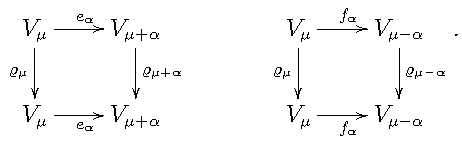
\includegraphics[width=0.3727\paperwidth]{images/L18-p153-morphisms.pdf}\end{figure}
\end{enumerate}
$C(\Psi)$自然具有刚性张量范畴结构。遗忘函子$\mathfrak F:C(\Psi)\to\operatorname{Vect}_k$将$(V_\mu)$送到$\bigoplus_\mu V_\mu$，是张量函子。定义$k$群$G_\Psi:=\operatorname{Aut}(\mathfrak F,\otimes)$，则它恰为根数据$\Psi$所对应的约化群。此外，由Tannaka形式理论，有张量范畴等价$C(\Psi)\simeq\operatorname{Rep}(G_\Psi)$。

回忆，$k$群$G$的\textbf{Borel子群}是极大连通可解子群。固定极大环面后，选取包含它的Borel子群，等价于选取一组正根。

现在设$k$为任意域，$k^s$、$\overline k$分别为可分闭包和代数闭包。若光滑连通$k$群$G$在代数闭包上的基变换$G_{\overline k}$按\eref{定义}{L18S2O1}为约化群，则称$G$约化。若连通约化$k$群$G$含有一个定义于$k$的Borel子群，则称它\textbf{拟分裂}。若$G$具有一个定义于$k$且在$k$上分裂的极大环面，则称它\textbf{分裂}。分裂群一定拟分裂。拟分裂性一般是相当强的限制，不过有：\idx{拟分裂群}\idx{分裂群}
% [Tutor Note: 原书 p153 定义约化 $k$ 群时用 $G\times_k k^s$（可分闭包），译文统一改用 $\overline k$；在本讲义涉及的有限域与曲线情形 $k^s=\overline k$，读者对照其他文献时注意这一差别。]
\begin{itemize}
\item 若$k$为有限域，则任意连通约化$k$群均拟分裂，这是Lang定理的结果。
\item 若$k$为非阿基米德局部域，则对每个连通约化$k$群$G$，存在非分歧扩张$L/k$，使$G$在$L$上拟分裂。
\item 若$k$为整体域，则对几乎所有素位$v$，$G\times_k k_v$拟分裂。
\end{itemize}
\sourcepage{154}
设$G$为连通约化$k$群，$S$为极大$k$-分裂环面，即$G$的$k$子环面，且$S$在$k$上分裂并对这一性质极大。$\dim S$称为$G$的\textbf{$k$-秩}。一般而言，$S$未必是$G$的极大环面。$\Phi(G,S)$称为$G$的\textbf{相对根系}\znote{绝对根系在代数闭包上取值，相对根系 ${}_k\Phi$ 只记录在 $k$ 上可见的根：取极大 $k$-分裂环面 $S$，把 $\operatorname{Lie}G$ 对 $S$ 对角化即得。$G$ 分裂时两者一致；非分裂时 ${}_k\Phi$ 可能不约化、根空间维数也可能大于 $1$。$k$-秩 $\dim S$ 衡量 $G$ 在 $k$ 上能分裂出多少环面，它正是 Satake 参数中与 $L$ 群相关的量。[来源：T.A. Springer, \textit{Reductive groups}, in \textit{Automorphic forms, representations and L-functions}, Proc. Symp. Pure Math. 33, Part 1, AMS 1979, pp.~3--27（本讲参考文献 [S]）。]}，记为${}_k\Phi$。相应的Lie代数分解为
\begin{equation}\tag{2.2}\label{L18eq22}\g=\g_0\oplus\bigoplus_{\alpha\in{}_k\Phi}\g_\alpha,\end{equation}
其中$\g_0$为中心化子$Z(S)$的Lie代数。若$G$在$k$上分裂，则$S$为$G$的极大环面，${}_k\Phi$与绝对根系$\Phi(G_{\overline k},S_{\overline k})$一致。一般而言，相对根系未必约化，根空间$\g_\alpha$也未必为一维。\idx{相对根系}
% [Tutor Note: 原书 p154 在此写绝对根系为 $\Phi(G(k),S(k))$；绝对根系应在代数闭包上取，即 $\Phi(G_{\overline k},S_{\overline k})$，译文已按此处理。]
\originalnumber{5}
\begin{definition}\label{L18S2O5}\idx{Langlands对偶群}
设$G$为根数据$\Psi=(X,\Phi,X^\vee,\Phi^\vee)$对应的分裂约化群。对偶根数据$\Psi^\vee$给出另一个分裂约化群$G^\vee$，称为$G$的\textbf{Langlands对偶群}\znote{对偶根数据 $\Psi^\vee$ 把特征标格与余特征标格互换，对应群 $G^\vee$（常记 $G^L$）。例：$\SL_n$ 与 $\\operatorname{PGL}_n$ 互为对偶，$\\operatorname{Sp}_{2n}$ 与 $\SO_{2n+1}$ 互为对偶，$\GL_n$ 自对偶。直观上 $G$ 与 $G^\vee$ 根系相同而中心、余中心互换，故 $G^\vee$ 的极大环面是 $G$ 极大环面的对偶环面。完整的 $L$ 群还带 Galois 部分，本讲只处理分裂情形。[来源：T.A. Springer, \emph{Reductive groups}, in \emph{Automorphic forms, representations and $L$-functions}, Proc. Symp. Pure Math. 33, Part 1, pp. 3--27, AMS, 1979（本讲参考文献 [S]）。]}，有时记为$G^L$。
\end{definition}
\originalnumber{6}
\begin{example}\label{L18S2O6}
\begin{center}\begin{tabular}{c|c}$G$&$G^L$\\\hline$\GL_n$&$\GL_n$\\$\SL_n$&$\operatorname{PGL}_n$\\$\operatorname{Sp}_{2n}$&$\SO_{2n+1}$\end{tabular}\end{center}
\end{example}
$k$群$G$的\textbf{有理表示}，由$k$向量空间$V$及$k$群同态$\rho:G\to\GL(V)$组成。关于分裂约化群的表示论，有下面的重要定理。若权$\lambda\in X=X^*(T)$满足$\langle\lambda,\alpha^\vee\rangle\ge0$，$\alpha\in\Delta$，则称$\lambda$为\textbf{支配权}。\idx{支配权}
% [Tutor Note: 原书 p154 作「A weight $\lambda\in X^\vee$ is dominant if $\langle\alpha,\lambda\rangle\ge0$」；支配权是 $X=X^*(T)$ 中的元素，条件应为 $\langle\lambda,\alpha^\vee\rangle\ge0$，译文已改正。]
\originalnumber{7}
\begin{theorem}\label{L18S2O7}
分裂约化群$G$的不可约有理表示的同构类，与$G$的支配权一一对应。
\end{theorem}
还要提及两个与约化性相关的定义。
\originalnumber{8}
\begin{definition}\label{L18S2O8}
\begin{enumerate}[label=(\arabic*)]
\item 若线性代数群$G$满足下列两个等价条件之一，则称它\textbf{线性约化}：
\begin{enumerate}[label=(\alph*)]
\item 每个有限维有理线性表示均完全可约，即是不可约表示的直和；
\sourcepage{155}
\item 对每个有理表示$\rho:G\to\GL(V)$及任意非零$\rho(G)$-不变向量$v\in V$，存在$\rho(G)$-不变线性函数$f$，满足$f(v)\ne0$。
% [Tutor Note: 原书 p155 (1)(b) 作 $f(W)\ne0$；此处 $W$ 未定义，应为 $f(v)\ne0$，译文已按 $f(v)\ne0$ 处理。]
\end{enumerate}
\item 若对每个有理表示$\rho:G\to\GL(V)$及任意非零不变向量$v\in V$，存在正次数的$\rho(G)$-不变齐次多项式函数$f$，使$f(v)\ne0$，则称$G$\textbf{几何约化}，亦称\textbf{半约化}。
% [Tutor Note: 原书 p155 (2) 作「non-constant polynomial function」；结合不变性可取其齐次分量，故与「正次数齐次多项式」等价，译文按后者表述。]
\end{enumerate}
\end{definition}
任意线性约化群都是约化群；线性代数群约化当且仅当几何约化。最后，若$\operatorname{char}(k)=0$，则$G$约化当且仅当$G$线性约化。
\section{环上的约化群}\label{L18S3}\idx{群概形}\idx{良约化}
可以将域$k$换成交换环$R$，得到\textbf{$R$上的仿射群概形}，简称\textbf{$R$群}。以$G(R)$表示$G$的$R$-点群，以$R[G]$表示$G$的坐标代数。若$R'$为$R$-代数，则基变换给出$R'$群$G\times_R R'$，其坐标代数为$R'[G]$。设$\mathfrak m$为$R$的极大理想，令$k(\mathfrak m)=R/\mathfrak m$。
\originalnumber{1}
\begin{definition}\label{L18S3O1}
设$G$为平坦且有限表示的$R$群。若$G\times_R k(\mathfrak m)$为光滑$k(\mathfrak m)$群，则称$G$在$\mathfrak m$处具有\textbf{良约化}。若$G$在所有极大理想处均具有良约化，则称$G$为\textbf{光滑}$R$群。
% [Tutor Note: 原书 p155 定义 3.1 作「$G\times_R k(\mathfrak m)$ is a $k(\mathfrak m)$-group」，漏了「光滑」；任何基变换都是 $k(\mathfrak m)$-群，故该条件只有读作「光滑 $k(\mathfrak m)$-群」才有意义，译文已补。]
\end{definition}
设$G$为域$k$上的$k$群，$R\subseteq k$为子环。若存在光滑$R$群$G_0$，满足$G\cong G_0\times_R k$，则称$G$\textbf{可定义于}$R$。
\originalnumber{2}
\begin{note}[L18S3O2]
由Chevalley定理，复连通半单群可定义于$\Z$。
\end{note}
还可以令$R=\A$为整体域$k$的阿代尔环。$G(\A)$为$\A$-点群，称为$G$的\textbf{阿代尔群}。由\sref{L4S2}，$G(\A)$局部紧，并包含对角嵌入的离散子群$G(k)$。
\sourcepage{156}
\needspace{5\baselineskip}\section{第18讲参考文献}\label{L18S4}
\begin{references}
\refitem{L18bibS}{S} T.A. Springer, \emph{Reductive groups}, in \emph{Automorphic forms, representations and L-functions}, Proc. Symp. Pure Math. 33, Part 1, pp. 3--27, AMS, 1979.
\end{references}

\addtocontents{toc}{\protect\newpage}
\chapter{其他约化群的Langlands对应II：Satake同构}\label{L19}\lecturedate{2020/04/22}\sourcepage{157}
\section{约化群的Bruhat分解}\label{L19S1}\idx{Bruhat分解}\idx{抛物子群}
设$k$为域，$G$为连通约化$k$群。$G$的\textbf{抛物子群}$P$是使$G/P$为射影簇的闭子群；等价地，在代数闭包上，$P$包含$G$的一个Borel子群。一般而言，$G$在$k$上未必拟分裂。因此，我们使用$G$的极小抛物$k$子群来代替Borel子群。任意两个极小抛物$k$子群都在$k$上共轭。事实上，若两个抛物$k$子群在$k$的某个扩域上共轭，则它们已经在$k$上共轭。

设$P$为$G$的极小抛物$k$子群。存在$G$的极大$k$分裂环面$S$，使$P$为$k$群的半直积$P=Z(S)\ltimes R_u(P)$，其中$Z(S)$表示$S$的中心化子，$R_u(P)$为$P$的幂幺根基，因而是正规子群。如\lref{L18}所述，${}_k\Phi=\Phi(G,S)$为相对根系，${}_kW$为$G$的相对Weyl群。此外，${}_kW\cong N(S)/Z(S)$，其中$N(S)$为$S$在$G$中的正规化子。$G$的Lie代数$\g$也有分解
\begin{equation}\tag{1.1}\label{L19eq11}\g=\g_0\oplus\bigoplus_{\alpha\in{}_k\Phi}\g_\alpha.\end{equation}
每个相对根$\alpha\in{}_k\Phi$都有相应的、由$S$正规化的幂幺$k$根子群$U_\alpha$；其Lie代数为$\bigoplus_{n\ge1}\g_{n\alpha}$，其中只取仍为根的$n\alpha$。可以给${}_k\Phi$选定一个正负划分，使$P$由$Z(S)$及正根对应的$U_\alpha$生成。记这一划分确定的基为${}_k\Delta$。对任意子集$\theta\subseteq{}_k\Delta$，以$P_\theta$表示$G$中由$Z(S)$及下述$U_\alpha$生成的子群：把$\alpha\in{}_k\Phi$写成单根的线性组合后，不属于$\theta$的单根的系数均非负。
% [Tutor Note: 原书 p157 作 $U_\alpha$ 的 Lie 代数为 $\g_\alpha$；相对根系若非约化（如 $BC_n$ 型），根子群 $U_\alpha$ 的 Lie 代数应为 $\bigoplus_{n\ge1}\g_{n\alpha}$（只取仍为根的 $n\alpha$），译文按后者处理。]
% [Tutor Note: 原书 p157–158 称 $P_\theta$ 是 $P$ 的子群；但 $\theta={}_k\Delta$ 时 $P_{{}_k\Delta}=G$ 显然不在 $P$ 中，故 $P_\theta$ 应理解为 $G$ 中由 $Z(S)$ 与这些 $U_\alpha$ 生成的子群，译文已改。]
\sourcepage{158}
于是$P_{{}_k\Delta}=G$、$P_\varnothing=P$；若$\theta_1\subseteq\theta_2$，则$P_{\theta_1}\subseteq P_{\theta_2}$。这些$P_\theta$称为包含$P$的$G$的\textbf{标准抛物子群}。$G$的任意抛物$k$子群都在$k$上共轭于唯一一个$P_\theta$。

令$U:=R_u(P)$。由${}_kW\cong N(S)/Z(S)$，对每个$w\in{}_kW$，可在$N(S)(k)$中选取代表元$n_w$。$G(k)$的\textbf{Bruhat分解}\znote{Bruhat 分解把 $G(k)$ 按双陪集 $U(k)n_wP(k)$ 拆成 $|{}_kW|$ 块，每块对应一个相对 Weyl 群元素。取 $k=\bar k$、$P=B$ 时，$Un_wB/B$ 是旗簇 $\mathcal B$ 中的仿射胞腔 $\A^{\ell(w)}$，其闭包给出 Bruhat 序，这是 Schubert 演算与相交上同调的起点。对 $p$ 进群，同一分解又是球面 Hecke 代数基 $c_\lambda$ 与 Satake 同构的组合基础。注意 $P$ 不必是 Borel、$U$ 也不必是极大幂幺子群，故该分解对任意抛物子群都成立，这使它能直接用于约化群的相对理论。[来源：nLab "Bruhat decomposition"，\url{https://ncatlab.org/nlab/show/Bruhat+decomposition}（Last revised 2024-07-11；2026-11-14 访问）。]}断言，$G(k)$为双陪集$U(k)n_wP(k)$的不交并，即
\begin{equation}\tag{1.2}\label{L19eq12}G(k)=\bigsqcup_{w\in{}_kW}U(k)n_wP(k).\end{equation}
按定义，$w(\alpha)(s)=\alpha(n_w^{-1}sn_w)$，$s\in S$，从而$n_w^{-1}U_\alpha n_w=U_{w^{-1}(\alpha)}$。
% [Tutor Note: 原书 p158 作 $n_w^{-1}U_\alpha n_w=U_{w(\alpha)}$；按本句给出的 $w(\alpha)(s)=\alpha(n_w^{-1}sn_w)$，正确关系为 $n_w U_\alpha n_w^{-1}=U_{w(\alpha)}$，等价地 $n_w^{-1}U_\alpha n_w=U_{w^{-1}(\alpha)}$，译文按正确写法处理。]定义
\[
U'_w:=\prod_{\substack{\alpha>0,\ w^{-1}(\alpha)<0\\\alpha/2\notin{}_k\Phi}}U_\alpha,
\qquad
U''_w:=\prod_{\substack{\alpha>0,\ w^{-1}(\alpha)>0\\\alpha/2\notin{}_k\Phi}}U_\alpha.
\]
乘积按适当顺序取。乘法给出簇的同构$U'_w\times U''_w\cong U$，并且$U''_w(k)n_wP(k)=n_wP(k)$。映射$U'_w(k)\times P(k)\to U(k)n_wP(k)$，$(u,p)\mapsto un_wp$，为双射。因此
% [Tutor Note: 原书 p158 定义 $U'_w,U''_w$ 时用条件 $w(\alpha)<0$、$w(\alpha)>0$ 且无 $\alpha/2$ 条件；译文改用 $w^{-1}(\alpha)$ 比较（与上式修正后的共轭关系一致），并补上 $\alpha/2\notin{}_k\Phi$（相对根系非约化时避免重复计算 $\g_{n\alpha}$）。]
\begin{equation}\tag{1.3}\label{L19eq13}(G/P)(k)=G(k)/P(k)=\bigsqcup_{w\in{}_kW}U'_w(k)n_wP(k)/P(k).\end{equation}
% [Tutor Note: 原书 p158 的 (1.3) 右端只写到 $U'_w(k)n_w$，漏了 $P(k)$ 与商 $/P(k)$；按上一段的双射，$U'_w(k)n_wP(k)/P(k)$ 才是 $G(k)/P(k)$ 的分解，译文已补。]
还具有以下性质。
\begin{itemize}
\item 若$k=\bar k$，则$P=B$为Borel子群，商$\mathcal B:=G/B$为$G$的\textbf{旗簇}\znote{旗簇 $\mathcal B=G/B$ 参数化 $G$ 的所有 Borel 子群（即「完全旗」）；$G=\GL_n$ 时它就是通常的完全旗流形，是射影簇。取定 $B$ 后，$\mathcal B$ 被 Bruhat 胞腔 $\mathcal B_w=Un_wB/B\cong\A^{\ell(w)}$ 分解，闭包 $\overline{\mathcal B_w}$ 是 Schubert 簇，维数等于 $w$ 的长度。它也是几何表示论中「$G$ 作用在自身 Borel 子群上」的紧化，几何 Satake 等价把它的等变层范畴与 $G^\vee$ 的表示联系起来。[来源：nLab "flag variety"，\url{https://ncatlab.org/nlab/show/flag+variety}（Last revised 2026-09-28；2026-11-14 访问）。]}。令$\mathcal B_w=U'_wn_wB/B=Un_wB/B$，则
\[\mathcal B_w\cong\A_k^{\ell(w)},\]
其中$\ell(w)$为$w$的长度：$w$可写成$\ell(w)$个单根反射的乘积，而任何这样的表达式都至少需要$\ell(w)$个反射。因此，此时\eqref{L19eq13}给出$\mathcal B$的胞腔分解。设$\overline{\mathcal B_w}$为$\mathcal B_w$的闭包，则
\[\overline{\mathcal B_w}=\bigsqcup_{y\preceq w}\mathcal B_y,\]
其中$\preceq$为\textbf{Bruhat序}，由关系
\[y\prec s_\alpha y\quad\text{当}\quad\ell(s_\alpha y)=\ell(y)+1\]
生成，这里$\alpha$可取任意根。于是，$y\preceq w$当且仅当$\ell(y)\le\ell(w)$，并且$w$的某个约化表达式$w=s_{\alpha_{\ell(w)}}\cdots s_{\alpha_1}$中存在一个子词，其乘积为$y$，该子词也可以取成$y$的约化表达式。
% [Tutor Note: 原书 p158 末作「存在 $w$ 的约化表达式使 $y=s_{\alpha_{\ell(y)}}\cdots s_{\alpha_1}$」，即要求 $y$ 是 $w$ 的约化表达式的**前缀**；该判据一般不对（如 $y$ 可以是中段子词），正确说法是「$y$ 的某个约化表达式是 $w$ 的约化表达式的子词」，译文按子词表述。]
\sourcepage{159}
\item 设$\theta\subseteq{}_k\Delta$，以$W_\theta$表示由$s_\alpha$，$\alpha\in\theta$，生成的${}_kW$的子群。对${}_k\Delta$的任意两个子集$\theta,\theta'$，有双陪集之间的双射
\[P_\theta(k)\backslash G(k)/P_{\theta'}(k)\cong W_\theta\backslash{}_kW/W_{\theta'}.\]
\end{itemize}\idx{旗簇}\idx{Bruhat序}
\originalnumber{1}
\begin{example}\label{L19S1O1}
我们给出一个非分裂环面的例子。定义
\[T_{\R}:=\{(x,y)\in\R^2\mid x^2+y^2=1\},\]
这是在$\R$上不分裂的一维环面。为了说明它是环面，可构造同构
\[f:T_{\R}\otimes_{\R}\C\xrightarrow{\sim}\C^\times,\qquad(x,y)\longmapsto x+yi.\]
注意，$T_{\R}\otimes_{\R}\C=\{(x,y)\in\C^2\mid x^2+y^2=1\}$，而逆映射$f^{-1}$为
\[\C^\times\ni z\longmapsto\left(\frac{z^2+1}{2z},\frac{z^2-1}{2iz}\right)\in T_{\R}\otimes_{\R}\C.\]
因此$T_{\R}\otimes_{\R}\C\cong\C^\times$。然而，它在$\R$上显然不同构于分裂环面$\mathbb G_m$：$T_{\R}(\R)$有界且紧，而$\R^\times$并不紧。
\end{example}
\section{球面Hecke代数}\label{L19S2}\idx{球面Hecke代数}\idx{卷积}
现在设$F$为非阿基米德局部域，$\OO_F$为$F$的整数环，$\mathfrak m\subset\OO_F$为极大理想，$\pi\in\mathfrak m$为素元。设$G$为$\OO_F$上的分裂约化群，即它具有一个在$\OO_F$上分裂的极大环面$T$，使$T(\OO_F)\cong(\OO_F^\times)^r$，其中$r$为$G$的秩。在$G(F)$上存在Haar测度$\mu$，可归一化为$\mu(G(\OO_F))=1$。

以$C_c(G)$表示\textbf{Schwartz函数}空间，即$G(F)$上具有紧支撑的局部常值复值函数所组成的空间。对任意两个Schwartz函数$f_1,f_2$，定义卷积积
\begin{equation}\tag{2.1}\label{L19eq21}(f_1*f_2)(g):=\int_{G(F)}f_1(x)f_2(x^{-1}g)\,d\mu(x).\end{equation}
于是$f_1*f_2$仍为Schwartz函数。
\sourcepage{160}
令$\mathcal H:=\mathcal H(G(F),G(\OO_F))$为$G(F)$上所有双$G(\OO_F)$不变的Schwartz函数组成的空间。卷积积$*$赋予$\mathcal H$一个代数结构，其单位元为$G(\OO_F)$的特征函数$1_{G(\OO_F)}$。$\mathcal H$称为\textbf{球面Hecke代数}\znote{球面 Hecke 代数 $\mathcal H(G(F),G(\OO_F))$ 由双 $G(\OO_F)$ 不变的紧支撑局部常值函数组成，乘法是卷积，单位元是 $G(\OO_F)$ 的特征函数。它是 $G(F)$ 的球面表示（含 $G(\OO_F)$-不变向量的不可约表示）所对应的交换 Hecke 代数：未分歧表示正对应到 $\mathcal H$ 到 $\C$ 的代数同态。$p$ 进群上它可视为有限 Hecke 代数的整体版本，也是 Satake 同构的出发空间。[来源：I. Satake, \textit{Theory of spherical functions on reductive algebraic groups over $p$-adic fields}, IHES Publ. Math. 18 (1963) 5--69（本讲参考文献 [S]）。]}，其中的函数称为球面函数。以$X$和$X^\vee$分别表示$T$的全部代数特征标和余特征标组成的格。有以下引理。
\originalnumber{1}
\begin{lemma}\label{L19S2O1}$T(F)/T(\OO_F)\cong X^\vee$。\end{lemma}
\begin{proof}
对每个$t\in T(F)$，存在唯一的余特征标$\xi(t)\in X^\vee$，使
\[\langle\lambda,\xi(t)\rangle=v(\lambda(t)),\qquad\lambda\in X,\]
其中$v:F\to\Z\cup\{+\infty\}$为$F$的归一化离散赋值。按定义，对$a\in F^\times$，有$\lambda\circ\xi(t)(a)=a^{\langle\lambda,\xi(t)\rangle}$。由于$T(F)\cong(F^\times)^r$，我们固定这样一个同构。写$t=(t_1,\ldots,t_r)$，其中$t_j=u_j\pi^{n_j}$，$u_j\in\OO_F^\times$。则$\xi(t)$为$a\mapsto(a^{n_1},\ldots,a^{n_r})$。于是$\xi(t)$平凡当且仅当所有$n_j=0$，亦即$t\in T(\OO_F)$。
% [Tutor Note: 原书 p160 引理 2.1 证明开头作「存在唯一的 $X^\vee\ni\xi(t):F^\times\to T(F),\ \pi\mapsto t$」，把余特征标与它在 $\pi$ 处的取值混在一起；$\xi(t)$ 应是 $X^\vee$ 中的余特征标（$G_m\to T$），译文按此处理。]
% [Tutor Note: 原书 p160 接着称「$\xi(t)$ 平凡当且仅当 $t\in\OO_F^\times$，等价于 $t_1=\cdots=t_r=1$」；$t\in\OO_F^\times$ 只是 $r=1$ 的情形，一般应为所有 $n_j=0$，即 $t\in T(\OO_F)=(\OO_F^\times)^r$，译文已改正。]

容易看出，$t\mapsto\xi(t)$给出满射$T(F)\to X^\vee$，其核为$T(\OO_F)$。
\end{proof}
记$\pi^{\mathbf n}=(\pi^{n_1},\ldots,\pi^{n_r})\in T(F)$，也就是$t=\pi^{\mathbf n}$时的$\xi(t)(\pi)$。选定正根后，记$D^+\subseteq\Z^r$为在上述坐标中对应于支配余权\znote{支配余权是满足 $\langle\alpha,\lambda\rangle\ge0$（对所有正根 $\alpha$）的余权 $\lambda\in X^\vee$。对分裂群，Cartan 分解的双陪集 $G(\OO_F)\lambda(\pi)G(\OO_F)$ 由支配余权唯一标记，因此 $\mathcal H$ 的基 $\{c_\lambda\}$ 与 $(X^\vee)^+$ 一一对应。几何上 $\lambda$ 记录极大环面在 $\pi$-进方向的位置；在对偶群一侧它对应支配权，而支配权与不可约有理表示一一对应，这正是 Satake 参数能读出表示不变量的原因。[来源：I. Satake, \textit{Theory of spherical functions on reductive algebraic groups over $p$-adic fields}, IHES Publ. Math. 18 (1963) 5--69（本讲参考文献 [S]）。]}的集合。有\textbf{Cartan分解}
\begin{equation}\tag{2.2}\label{L19eq22}G(F)=\bigsqcup_{\mathbf n\in D^+}G(\OO_F)\pi^{\mathbf n}G(\OO_F).\end{equation}
% [Tutor Note: 原书 p160 的 Cartan 分解写作对 $\mathbf n\in\Z^r_{\ge0}$ 求和；$\Z^r_{\ge0}$ 在 $X^\vee$ 的整基下只对应「非负坐标」的余权，双陪集实际由支配余权（一个 Weyl 室）标记，译文改用 $D^+$。]
另一种说法是：给对偶根系$\Phi(G,T)^\vee$选定基$\Delta^\vee$，便得到支配余权集合
\[(X^\vee)^+=\{\lambda\in X^\vee\mid\langle\alpha,\lambda\rangle\ge0,\ \alpha\in\Delta\}.\]
所选的正根同时确定Langlands对偶群$G^L$的一个Borel子群。\eqref{L19eq22}可写成
\[G(F)=\bigsqcup_{\lambda\in(X^\vee)^+}G(\OO_F)\lambda(\pi)G(\OO_F).\]
因此$G(\OO_F)\backslash G(F)/G(\OO_F)\cong(X^\vee)^+$，而$\mathcal H$具有基$\{c_\lambda\}_{\lambda\in(X^\vee)^+}$，其中$c_\lambda$为双陪集$G(\OO_F)\lambda(\pi)G(\OO_F)$的特征函数。\idx{Cartan分解}\idx{支配余权}
\originalnumber{2}
\begin{proposition}\label{L19S2O2}球面Hecke代数$\mathcal H$是交换的。\end{proposition}
\sourcepage{161}
\begin{proof}
只需确定结构常数
\[c_\lambda*c_\gamma=\sum_{\nu\in(X^\vee)^+}c^\nu_{\lambda\gamma}c_\nu.\]
为简化公式，记$K=G(\OO_F)$。按定义，对$a\in K\nu(\pi)K$，有
\begin{align*}
c^\nu_{\lambda\gamma}&=(c_\lambda*c_\gamma)(a)=\int_{G(F)}c_\lambda(x)c_\gamma(x^{-1}a)\,d\mu(x)\\
&=\mu\bigl(K\lambda(\pi)K\cap aK\gamma(\pi)^{-1}K\bigr)\\
&=\left|\bigl(K\lambda(\pi)K\cap aK\gamma(\pi)^{-1}K\bigr)/K\right|.
\end{align*}
可以选择$G$的Cartan对合$\sigma$。例如，对某个把Borel子群映入上三角矩阵群的嵌入$G\hookrightarrow\GL_n$，可取$\sigma(g)=(g^{\mathsf T})^{-1}$，其中$g^{\mathsf T}$表示转置。$\sigma$为$G$的自同构，满足：
\begin{enumerate}[label=\arabic*.]
\item $\sigma(g_1g_2)=\sigma(g_1)\sigma(g_2)$；
\item $\sigma(T)=T$，且$\sigma(t)=t^{-1}$，$t\in T$；
\item $\sigma(K)=K$，所以对任意可测集$V\subseteq G(F)$，$\mu(V)=\mu(\sigma(V))$。
\end{enumerate}
令$\widetilde a=\sigma(a)^{-1}\in K\nu(\pi)K$，则
\[\sigma\bigl(K\lambda(\pi)K\cap aK\gamma(\pi)^{-1}K\bigr)=K\lambda(\pi)^{-1}K\cap\widetilde a^{-1}K\gamma(\pi)K.\]
容易得到
\begin{align*}
c^\nu_{\lambda\gamma}&=\mu\bigl(K\lambda(\pi)K\cap aK\gamma(\pi)^{-1}K\bigr)\\
&=\mu\bigl(\sigma(K\lambda(\pi)K\cap aK\gamma(\pi)^{-1}K)\bigr)\\
&=\mu\bigl(K\lambda(\pi)^{-1}K\cap\widetilde a^{-1}K\gamma(\pi)K\bigr)\\
&=\mu\bigl(\widetilde aK\lambda(\pi)^{-1}K\cap K\gamma(\pi)K\bigr)=c^\nu_{\gamma\lambda}.
\end{align*}
\end{proof}
设$U$为由$T$正规化的一个Borel子群的幂幺根基。有以下\textbf{Iwasawa分解}：
\begin{equation}\tag{2.3}\label{L19eq23}G(F)=\bigsqcup_{\lambda\in X^\vee}G(\OO_F)\lambda(\pi)U(F).\end{equation}\idx{Iwasawa分解}
\sourcepage{162}
\section{Satake同构}\label{L19S3}\idx{Satake同构}
$F,\OO_F,G,\mathcal H$等仍如前。我们已经看到，$\mathcal H$由$c_\lambda$，$\lambda\in(X^\vee)^+$，张成。若$G=T$为秩$r$的$\OO_F$分裂环面，则$G(\OO_F)\cong(\OO_F^\times)^r$，且
\[c_\lambda*c_\gamma=c_{\lambda+\gamma}.\]
因而存在代数同构
\[\mathcal H(T(F),T(\OO_F))\xrightarrow{\sim}\C[x_1^{\pm1},\ldots,x_r^{\pm1}]\cong\C[X^\vee],\]
把$\sum C_\lambda c_\lambda$送到$\sum C_\lambda x^\lambda$。这里$x^\lambda=x_1^{\lambda_1}\cdots x_r^{\lambda_r}$，$\lambda=\lambda_1\gamma_1+\cdots+\lambda_r\gamma_r$，$\gamma_1,\ldots,\gamma_r$为余特征标格$X^\vee$的一组整基，$C_\lambda\in\C$。
% [Tutor Note: 原书 p162 称 $\gamma_1,\ldots,\gamma_r$ 是「all the simple coroots」；单余根一般只生成根格 $Q^\vee$，不构成 $X^\vee$ 的整基（如 $\GL_n$ 的 $X^\vee\cong\Z^n$ 需 $n$ 个元素而只有 $n-1$ 个单余根），译文改为 $X^\vee$ 的一组整基。]

然而，对一般的$G$，映射$c_\lambda\mapsto x^\lambda$并不是从$\mathcal H$到$\C[X^\vee]$的代数同态。Satake构造了另一个映射$\mathcal H\to\C[X^\vee]$，并证明了下面称为\textbf{Satake同构}\znote{Satake 同构断言球面 Hecke 代数同构于 Weyl 群不变的多项式环：$\mathcal H\cong\C[X^\vee]^W$。代数侧看，它把 $G(F)$ 的未分歧表示（即 $\mathcal H$ 的代数同态）与半单共轭类（即 $\C[X^\vee]^W$ 的极大理想）对应起来，因此未分歧表示由半单 $L$-参数决定，这就是「Satake 参数」。显式同构 $f\mapsto\widehat f$ 由 Fourier 变换在带状球函数上的取值给出，正是本讲末尾构造的内容。[来源：I. Satake, \textit{Theory of spherical functions on reductive algebraic groups over $p$-adic fields}, IHES Publ. Math. 18 (1963) 5--69（本讲参考文献 [S]）。]}的结果。
\originalnumber{1}
\begin{theorem}\label{L19S3O1}存在代数同构$\mathcal H\xrightarrow{\sim}\C[X^\vee]^W$，其中$W$为Weyl群。\end{theorem}
\originalnumber{2}
\begin{note}[L19S3O2]
实际上，可将$\C[X^\vee]$看作$X\otimes\C$上的指数多项式。在同构$\C[X^\vee]\cong\C[x_1^{\pm1},\ldots,x_r^{\pm1}]$下，$x_i$对应的函数为
\[x_i(\alpha)=e^{-\langle\alpha,\gamma_i\rangle},\qquad\alpha\in X\otimes\C,\]
其中$\gamma_1,\ldots,\gamma_r$为上述整基。换言之，同构$\mathcal H(T(F),T(\OO_F))\xrightarrow{\sim}\C[X^\vee]$由$c_\lambda\mapsto e^\lambda$给出。因此Weyl群$W$自然作用于$\C[X^\vee]$。
% [Tutor Note: 原书 p162 注记 3.2 作 $x_i(\alpha)=e^{\langle\alpha,\gamma_i\rangle}$；与本讲 (3.2)、(3.3) 采用的 $e^{-\langle s,\lambda\rangle}$ 约定相差一个负号，译文统一取 $x_i(\alpha)=e^{-\langle\alpha,\gamma_i\rangle}$。]
\end{note}
我们想简要说明\eref{定理}{L19S3O1}的证明。以下遵循\bref{L19S}{S}，先给出一个定义。
\originalnumber{3}
\begin{definition}\label{L19S3O3}
若$G(F)$上的连续复值函数$\omega$满足以下条件，则称其为$G(F)$上相对于$G(\OO_F)$的\textbf{带状球函数}\znote{带状球函数是 $G(F)$ 上双 $G(\OO_F)$ 不变、在单位元取 $1$、且是每个 $f\in\mathcal H$ 所定义卷积算子的特征函数的连续函数。它与「球面表示」一一对应：在不可约球面表示 $(\pi,V)$ 中取 $G(\OO_F)$-不变向量 $v$，矩阵元 $g\mapsto\langle\pi(g)v,v\rangle$ 就是带状球函数；反过来 $\omega$ 的 $E_f$ 给出 $\mathcal H$ 的一个特征。故 $\Omega$ 与 $\mathcal H$ 的谱（未分歧表示的 Satake 参数）是同一件事。[来源：I. Satake, \textit{Theory of spherical functions on reductive algebraic groups over $p$-adic fields}, Publ. Math. IHÉS 18 (1963) 5--69，第 1--2 节（本讲参考文献 [S]）。]}（zonal spherical function，以下简记为z.s.f.）：
\begin{enumerate}[label=(\roman*)]
\item $\omega$双$G(\OO_F)$不变；
\item $\omega(1)=1$；
\sourcepage{163}
\item 对任意$f\in\mathcal H$，$\omega$为$f$所定义积分算子的特征函数，即
\[f*\omega(g)=\int_{G(F)}f(x)\omega(x^{-1}g)\,d\mu(x)=E_f\omega(g),\qquad g\in G(F),\]
其中$E_f\in\C$。记$\widehat\omega(f)=E_f$，则
\begin{equation}\tag{3.1}\label{L19eq31}\widehat\omega(f)=\int_{G(F)}f(x)\omega(x^{-1})\,d\mu(x).\end{equation}
\end{enumerate}
\end{definition}\idx{带状球函数}
\eqref{L19eq31}中的映射$\widehat\omega$为从$\mathcal H$到$\C$的满代数同态。记$\Omega:=\Omega(G(F),G(\OO_F))$为$G(F)$上相对于$G(\OO_F)$的所有带状球函数的集合。

如何构造这样的函数？设$\chi$为$T(F)$的拟特征标，即从$T(F)$到$\C^\times$的连续同态，并满足$\chi(T(\OO_F))=1$。以$\delta(h)=|\det(\operatorname{Ad}(h)|_{\operatorname{Lie}U})|$表示相应的模特征标。借助\eqref{L19eq23}中的Iwasawa分解，$\chi$在$G(F)$上确定一个良定义的、归一化的复值函数$f_\chi$：
\[f_\chi(khu)=\delta(h)^{-1/2}\chi(h),\qquad k\in G(\OO_F),\ u\in U(F),\ h\in T(F).\]
% [Tutor Note: 原书 p163 定义 $f_\chi(khu)=\chi(h)$，未作归一化；为使其积分为带状球函数（$\omega_\chi(1)=1$ 且 $f*\omega=E_f\omega$ 成立），译文改用归一化的 $\delta(h)^{-1/2}\chi(h)$（$\delta$ 为 $T$ 的模特征标），与 Satake 的标准约定一致。]
从定义容易看出，若$g\in G(\OO_F)U(F)$，则$f_\chi(g)=1$。定义
\[\omega_\chi(g)=\int_{G(\OO_F)}\overline{f_\chi(x)}f_\chi(g^{-1}x)\,d\mu(x)=\int_{G(\OO_F)}f_\chi(g^{-1}x)\,d\mu(x).\]
则$\omega_\chi$为$G(F)$上相对于$G(\OO_F)$的带状球函数。

由\eref{引理}{L19S2O1}，这样的拟特征标$\chi$由$\chi(\pi^\lambda)$唯一确定，其中$\pi^\lambda=\lambda(\pi)$，$\lambda\in X^\vee$。因此可找到$s\in X\otimes\C$，使
\begin{equation}\tag{3.2}\label{L19eq32}\chi(\pi^\lambda)=e^{-\langle s,\lambda\rangle}.\end{equation}
这样的$s$在模$2\pi iX'$的意义下唯一，其中
\[X'=\{s\in X\otimes\C\mid\langle s,\lambda\rangle\in\Z,\ \lambda\in X^\vee\}=X.\]
% [Tutor Note: 原书 p163 作 $X\subset X'=\{s\in X\otimes\C\mid\langle s,\lambda\rangle\in\Z,\ \forall\lambda\in X^\vee\}$，只断言 $X$ 含于 $X'$；由 $X$ 与 $X^\vee$ 的配对完美，实际有 $X'=X$，译文直接写出等号。]
当$s,\chi$满足\eqref{L19eq32}时，记$\omega_s=\omega_\chi$。有以下引理。
\originalnumber{4}
\begin{lemma}\label{L19S3O4}
\begin{enumerate}[label=(\arabic*)]
\item $\omega_{-s}(g)=\omega_s(g^{-1})$。
\item 对任意$w\in W$，$\omega_{ws}=\omega_s$。
\end{enumerate}
\end{lemma}
\sourcepage{164}
第一条可以直接证明，但第二条的证明并不平凡，可见\bref{L19S}{S}。
\originalnumber{5}
\begin{theorem}\label{L19S3O5}
$G(F)$上相对于$G(\OO_F)$的所有带状球函数都可写成$\omega=\omega_s$，其中$s\in X\otimes\C$；并且$\omega_s=\omega_{s'}$当且仅当$s,s'$在$W\ltimes(2\pi iX')$的作用下等价。特别地，$\Omega$与商空间
\[(X\otimes\C)\big/\bigl(W\ltimes(2\pi iX')\bigr)\]
在复解析意义下同构。
\end{theorem}
现在，对任意$f\in\mathcal H$，定义其\textbf{Fourier变换}$\widehat f$为$X\otimes\C$上的函数
\begin{equation}\tag{3.3}\label{L19eq33}\widehat f(s):=\widehat\omega_s(f)=\int_{G(F)}f(x)\omega_s(x^{-1})\,d\mu(x).\end{equation}
在\eqref{L19eq11}所给出的Lie代数分解中，令$\mathfrak n=\bigoplus_{\alpha>0}\g_\alpha$。以$\operatorname{Ad}_{\mathfrak n}$表示$T$的伴随表示在$\mathfrak n$上的限制。定义
\[\delta:T(F)\to\R_{>0},\qquad h\longmapsto|\det(\operatorname{Ad}_{\mathfrak n}(h))|,\]
其中$|\cdot|$为赋值$v$在$F$上诱导的绝对值。$\delta$也称为$T$上的\textbf{模特征标}。定义
\[\widetilde f(h)=\delta(h)^{1/2}\int_{U(F)}f(hu)\,d\mu_U(u),\qquad h\in T(F),\]
其中$\mu_U$为$U(F)$上的Haar测度，归一化为$\mu_U(U(\OO_F))=1$。于是
\[\widehat f(s)=\sum_{\lambda\in X^\vee}\widetilde f(\pi^\lambda)e^{-\langle s,\lambda\rangle}.\]
最后，\eref{定理}{L19S3O1}中的同构显式地由$f\mapsto\widehat f$给出。\idx{模特征标}
\needspace{5\baselineskip}\section{第19讲参考文献}\label{L19S4}
\begin{references}
\refitem{L19S}{S} I. Satake, \textit{Theory of spherical functions on reductive algebraic groups over p-adic fields}, IHES Publ. Math. 18 (1963) 5--69.
\refitem{L19Sp}{S} T.A. Springer, \textit{Reductive groups}, in \textit{Automorphic forms, representations and L-functions}, Proc. Symp. Pure Math. 33, Part 1, pp. 3--27, AMS, 1979.
\end{references}

\chapter{其他约化群的Langlands对应III：对应的表述}\label{L20}\lecturedate{2020/04/27}\sourcepage{165}
设$F$为非阿基米德局部域，$\OO_F$为其整数环。% [Tutor Note: 原书 p165 作「Let $F$ be a local field」（未排除阿基米德情形）；本讲只用到非阿基米德情形，译文按此收紧。]设$G$为$F$上的分裂约化群，并选取其分裂约化$\OO_F$模型和在$\OO_F$上定义的极大分裂环面$T$。以$X,X^\vee$分别表示$T$的代数特征标格和余特征标格。\lref{L19}介绍了Satake同构
\begin{equation}\tag{0.1}\label{L20eq01}\mathcal H=\mathcal H(G(F),G(\OO_F))\cong\C[X^\vee]^W.\end{equation}
这一同构把每个$f\in\mathcal H$送到它的Fourier变换$\widehat f$。

以$G^L$表示$G$的Langlands对偶群，$T^L$为其中的极大环面。于是$X,X^\vee$分别是$T^L$的余特征标格和特征标格。由\eref{定理}{L18S2O7}，$G^L(\C)$的不可约有理表示与其支配权一一对应。另一方面，$G^L(\C)$约化，因而线性约化，每个有限维有理表示都是不可约表示的直和。
\section{\texorpdfstring{$\C[X^\vee]^W$}{C[X∨]的W不变环}的两组基}\label{L20S1}\idx{Weyl特征标}\idx{表示环}
由\eqref{L20eq01}中的Satake同构，$\{\widehat c_\lambda\}_{\lambda\in(X^\vee)^+}$给出$\C[X^\vee]^W$的一组基。

另一方面，对应于支配权$\lambda$的$G^L(\C)$的不可约表示$V_\lambda$，其\textbf{Weyl特征标}定义为
\begin{equation}\tag{1.1}\label{L20eq11}
\operatorname{Ch}(V_\lambda):=\sum_{\gamma\in X^\vee}\dim V_\lambda(\gamma)e^\gamma
=\frac{\sum_{w\in W}(-1)^{\ell(w)}e^{w(\lambda+\kappa^\vee)-\kappa^\vee}}{\prod_{\alpha^\vee\in\Phi^\vee_+}(1-e^{-\alpha^\vee})}.
\end{equation}
% [Tutor Note: 原书 p165 的 (1.1) 分母作 $\sum_{\alpha^\vee\in\Phi^\vee_+}(1-e^{-\alpha^\vee})$（求和号），应为乘积 $\prod$；译文按正确写法处理。]
\sourcepage{166}
这里，作为$T^L(\C)$模，$V_\lambda$具有权空间分解$V_\lambda=\bigoplus_{\gamma\in X^\vee}V_\lambda(\gamma)$，而$\kappa^\vee=\frac12\sum_{\alpha^\vee\in\Phi^\vee_+}\alpha^\vee$。容易看出，$\operatorname{Ch}(V_\lambda)$为$W$不变量，并构成$\C[X^\vee]^W$的一组基。还可为任意有限维有理表示定义Weyl特征标，使
\[\operatorname{Ch}(V_1\oplus V_2)=\operatorname{Ch}(V_1)+\operatorname{Ch}(V_2).\]
因此映射$V\mapsto\operatorname{Ch}(V)\in\C[X^\vee]^W$给出复化表示环$\operatorname{Rep}G^L(\C)\otimes_{\Z}\C$与$\C[X^\vee]^W$的同构。

现在，$\C[X^\vee]^W$有两组基$\{\widehat c_\lambda\}_{\lambda\in(X^\vee)^+}$和$\{\operatorname{Ch}(V_\lambda)\}_{\lambda\in(X^\vee)^+}$。写成
\begin{equation}\tag{1.2}\label{L20eq12}\operatorname{Ch}(V_\lambda)=\sum_{\gamma\in(X^\vee)^+}d_{\lambda\gamma}\widehat c_\gamma.\end{equation}
\originalnumber{1}
\begin{lemma}\label{L20S1O1}设$d_{\lambda\gamma}$如\eqref{L20eq12}。除非$\gamma\le\lambda$，否则$d_{\lambda\gamma}=0$。\end{lemma}
\begin{proof}
由\lref{L19}末给出的公式，
\begin{align*}
\widehat c_\gamma&=\sum_{\nu\in X^\vee}\widetilde c_\gamma(\pi^\nu)e^\nu
=\sum_{\nu\in(X^\vee)^+}\widetilde c_\gamma(\pi^\nu)\left(\sum_{w\in W/W_\nu}e^{w(\nu)}\right)\\
&=\sum_{\nu\in(X^\vee)^+}\delta(\pi^\nu)^{1/2}\int_{U(F)}c_\gamma(\pi^\nu u)\,d\mu_U(u)\left(\sum_{w\in W/W_\nu}e^{w(\nu)}\right),
\end{align*}
% [Tutor Note: 原书 p166 的 (1.2) 证明中作 $e^{-\nu}$、$e^{-w(\nu)}$，译文用 $e^{\nu}$、$e^{w(\nu)}$，与上一讲 $c_\lambda\mapsto e^\lambda$ 的约定一致。]
其中$\delta$为$T(F)$上的模特征标，$W_\nu$为$\nu$在$W$中的稳定子群，$U(F)$为所选正根对应的$G$的Borel子群$B$的幂幺根基，$\mu_U$为$U(F)$上的Haar测度，归一化为$\mu_U(U(\OO_F))=1$。按定义，
% [Tutor Note: 原书 p166 称 $U(F)$ 为「与 $G^L$ 的正根选取相对应的 Borel 子群的幂幺根基」，此处应为 $G$ 的正根（$\delta$ 由 $G$ 的根空间计算）；译文按正确写法处理。]
\[\widetilde c_\gamma(\pi^\nu)=\delta(\pi^\nu)^{1/2}\mu_U\bigl(\pi^{-\nu}G(\OO_F)\pi^\gamma G(\OO_F)\cap U(F)\bigr).\]
由下面的\eref{引理}{L20S1O2}，除非$\nu\le\gamma$，否则$\widetilde c_\gamma(\pi^\nu)=0$。因此，只有有限多个$\nu\in(X^\vee)^+$使$\widetilde c_\gamma(\pi^\nu)\ne0$。

此外，$\widetilde c_\gamma(\pi^\gamma)\ne0$，因为
\[\pi^\gamma U(F)\cap G(\OO_F)\pi^\gamma G(\OO_F)\supseteq\pi^\gamma\bigl(U(F)\cap G(\OO_F)\bigr),\]
且$\mu_U(U(F)\cap G(\OO_F))=\mu_U(U(\OO_F))=1$。

另一方面，对支配权$\nu$，只有$\nu\le\lambda$时，$\dim V_\lambda(\nu)$才可能非零。由两组基的三角形展开及\eqref{L20eq12}右端的有限性，得到：对任何不满足$\gamma\le\lambda$的$\gamma$，都有$d_{\lambda\gamma}=0$。
\end{proof}
\originalnumber{2}
\begin{lemma}\label{L20S1O2}
若$\pi^\nu U(F)\cap G(\OO_F)\pi^\gamma G(\OO_F)\ne\varnothing$，其中$\nu\in X^\vee$、$\gamma\in(X^\vee)^+$，则$\nu\le\gamma$。
\end{lemma}
\sourcepage{167}
\eref{引理}{L20S1O2}的证明见\bref{L20S}{S}第7.2、7.3节。

按定义，$\delta(\pi^\nu)^{1/2}=q^{-\langle\kappa,\nu\rangle}$，其中$\kappa=\frac12\sum_{\alpha\in\Phi_+}\alpha$，$q=|\OO_F/\mathfrak m|$。对$\gamma\in(X^\vee)^+$，定义
\[a^\nu_\gamma:=\mu_U\bigl(\pi^{-\nu}G(\OO_F)\pi^\gamma G(\OO_F)\cap U(F)\bigr).\]
若$g$属于这一交集，则整个右陪集$gU(\OO_F)$也属于交集。因此$a^\nu_\gamma$是非负整数；它或者为零，或者至少为$1$。对任意$w\in W$，还有
\[q^{-\langle\kappa,\nu\rangle}a^\nu_\gamma=q^{-\langle\kappa,w(\nu)\rangle}a^{w(\nu)}_\gamma,\]
以及
\begin{equation}\tag{1.3}\label{L20eq13}\widehat c_\gamma=\sum_{\nu\in X^\vee}q^{-\langle\kappa,\nu\rangle}a^\nu_\gamma e^\nu.\end{equation}
% [Tutor Note: 原书 p167 的 (1.3) 作 $e^{-\nu}$，译文用 $e^{\nu}$，同上一条的符号约定。]
有以下Lusztig的定理，见\bref{L20L}{L}。
\originalnumber{3}
\begin{theorem}\label{L20S1O3}
设$d_{\lambda\gamma}$如\eqref{L20eq12}，则$p_{\lambda\gamma}:=q^{\langle\kappa,\lambda\rangle}d_{\lambda\gamma}$为$q$的多项式，并且$p_{\lambda\gamma}(1)=\dim V_\lambda(\gamma)$。
\end{theorem}
有
\begin{equation}\tag{1.4}\label{L20eq14}\sum_{\gamma\in(X^\vee)^+}p_{\lambda\gamma}a^\nu_\gamma=q^{\langle\kappa,\lambda+\nu\rangle}\dim V_\lambda(\nu).\end{equation}
由于不满足$\gamma\le\lambda$时$p_{\lambda\gamma}=0$，而只要存在$w\in W$使$w(\nu)\not\le\gamma$，就有$a^\nu_\gamma=0$，所以$p_{\lambda\gamma}a^\nu_\gamma\ne0$仅可能发生在对所有$w\in W$均有$w(\nu)\le\gamma\le\lambda$的情形。令$w_0$为Weyl群的最长元，取$\nu=w_0\lambda$，得到
\[p_{\lambda\lambda}a^{w_0\lambda}_\lambda=\dim V_\lambda(w_0\lambda)=1=p_{\lambda\lambda}(1).\]
% [Tutor Note: 原书 p167 取 ν=−λ，本处取 ν=w_0λ；两者由 w_0 置换对应，结论一致。]
由于$a^{w_0\lambda}_\lambda\ge1$，有
\[\begin{cases}p_{\lambda\lambda}=\dim V_\lambda(\lambda)=p_{\lambda\lambda}(1)=1,\\a^{w_0\lambda}_\lambda=1.\end{cases}\]
于是矩阵$(p_{\lambda\gamma})$为单位上三角矩阵，\eqref{L20eq14}中的线性方程的解可表示为$q$的多项式。因此证明了以下推论。
\originalnumber{4}
\begin{corollary}\label{L20S1O4}$a^\nu_\gamma$为$q$的多项式。\end{corollary}
回忆，$\mathcal H$的结构常数定义为
\[c_\lambda*c_\gamma=\sum_{\beta\in(X^\vee)^+}c^\beta_{\lambda\gamma}c_\beta,\qquad\lambda,\gamma\in(X^\vee)^+.\]
\sourcepage{168}
\originalnumber{5}
\begin{corollary}\label{L20S1O5}$c^\beta_{\lambda\gamma}$为$q$的多项式。\end{corollary}
\begin{proof}
\eqref{L20eq01}中的Satake同构为代数同态，所以
\[\sum_{\beta\in(X^\vee)^+}c^\beta_{\lambda\gamma}\widehat c_\beta=\widehat{c_\lambda*c_\gamma}=\widehat c_\lambda\,\widehat c_\gamma.\]
因此
\[\sum_{\beta\in(X^\vee)^+}c^\beta_{\lambda\gamma}q^{-\langle\kappa,\nu\rangle}a^\nu_\beta=\sum_{\nu_1+\nu_2=\nu}q^{-\langle\kappa,\nu\rangle}a^{\nu_1}_\lambda a^{\nu_2}_\gamma,\]
从而
\[\sum_{\beta\in(X^\vee)^+}c^\beta_{\lambda\gamma}a^\nu_\beta=\sum_{\nu_1+\nu_2=\nu}a^{\nu_1}_\lambda a^{\nu_2}_\gamma.\]
由\eref{推论}{L20S1O4}，右端为$q$的多项式。取$\nu=w_0\eta$时，矩阵$(a^{w_0\eta}_\beta)$也是单位上三角的，因此逐项求解可知$c^\beta_{\lambda\gamma}$为$q$的多项式。
\end{proof}

\section{Langlands函子性}\label{L20S2}\idx{Langlands函子性}\idx{L群}
上一讲定义的带状球函数，见\eref{定义}{L19S3O3}，正是归一化的Hecke特征函数。% [Tutor Note: 原书 p168 引作「Definition 3.4 in Lecture 19」，实为定义 3.3（该讲顺序为定理 3.1、注记 3.2、定义 3.3）；译文引用正确。]
由\eref{定理}{L19S3O5}，这些特征函数与
\[(X\otimes\C)\big/\bigl(W\ltimes(2\pi iX')\bigr),\qquad X'=\{s\in X\otimes\C\mid\langle s,\lambda\rangle\in\Z,\ \lambda\in X^\vee\},\]
中的元素一一对应。
\originalnumber{1}
\begin{note}[L20S2O1]
上述商空间可看作$G^L(\C)$的半单共轭类集合。选取$X$的一组基$x_1,\ldots,x_r$，把$s=\sum b_jx_j\in X\otimes\C$对应到$G^L(\C)$中的元素$\prod_jx_j(e^{-b_j})$。注意，$x_j\in X$可视为对偶环面$T^L$的一参数余特征标。该对应诱导上述商空间与$G^L(\C)$半单共轭类集合之间的同构。
\end{note}
% [Tutor Note: 原书 p168 的注记 2.1 作 $\prod_j x_j(e^{b_j})$（译文用 $e^{-b_j}$，符号约定同上），并称 $x_i\in X$「可视为 $T$ 的一参数子环面」，此处应为对偶环面 $T^L$ 的一参数子群；译文按正确写法处理。]
每个Hecke特征函数$\omega$给出同态$\mathcal H\to\C$，$f\mapsto\widehat\omega(f)$。此外，有以下交换图：
\begin{figure}[H]\centering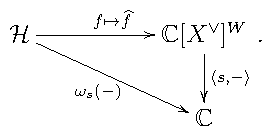
\includegraphics[width=0.2192\paperwidth]{images/L20-p168-Satake.pdf}\end{figure}
\sourcepage{169}
综合上述结果，有以下定理。
\originalnumber{2}
\begin{theorem}\label{L20S2O2}
球面Hecke代数$\mathcal H(G(F),G(\OO_F))$同构于$\operatorname{Rep}G^L(\C)\otimes_{\Z}\C$，其中$G^L(\C)$为$G$的Langlands对偶群。$\C$代数同态$\mathcal H(G(F),G(\OO_F))\to\C$的集合与$G^L(\C)$的半单共轭类集合之间存在双射。
\end{theorem}
\eref{定理}{L20S2O2}可看作非阿基米德局部域上非分歧情形的局部Langlands对应\znote{局部 Langlands 对应猜想：$G(F)$ 的不可约光滑表示应与 $L$ 参数（$W_F\times\SL_2$ 到 $G^L$ 的连续同态类）一一对应，并使两边的 $L$ 函数与 $\varepsilon$ 因子相符。未分歧情形即本讲定理 2.2：表示由半单共轭类（Satake 参数）决定，而对任意分裂约化群这一情形已经成立。$\GL_n$ 的一般情形是已知定理。它是整体 Langlands 对应的局部构件。[来源：S. Gelbart, \textit{An elementary introduction to the Langlands program}, Bull. Amer. Math. Soc. 10 (1984) 177--219（本讲参考文献 [G]）。]}。之所以称为非分歧情形，是因为定义带状球函数的拟特征标在$T(\OO_F)$上的限制为平凡特征标。关于局部Langlands猜想，还有其他结果，见\bref{L20BG}{BG}。

但在整体情形，对应关系无法像$\GL_n$情形那样清晰地一一配对。我们将简要介绍\textbf{Langlands函子性}\znote{Langlands 函子性说：每个 $L$ 同态 $f:G^L\to G'^L$ 都应诱导自守表示的转移，把 $G$ 的自守表示送到 $G'$ 的自守表示，并使两边的 $L$ 函数一致。它把 Langlands 猜想统一到约化群：取 $G'=\GL_n$ 可把一般 $G$ 的 $L$ 函数归约到 $\GL_n$ 的已知理论，取 $G$ 平凡则回到互反猜想。已证情形包括内形之间的 Jacquet--Langlands 对应、经典群的内窥理论，以及对称幂函子性的部分情形。[来源：nLab "Langlands functoriality"，\url{https://ncatlab.org/nlab/show/Langlands+functoriality}（Last revised 2022-11-23；2026-11-14 访问）。]}，它最终把Langlands猜想推广到约化群。也可参看\bref{L20BG}{BG}或\bref{L20G}{G}。

设$\A_F$为整体域$F$的阿代尔环。先回顾对$G=\GL_n$已经讨论的结果。
\begin{enumerate}[label=\arabic*.]
\item \textbf{从局部到整体。}每个$G(\A_F)$的不可约可容许表示都可写为局部不可约可容许表示$\rho_v$的限制张量积$\bigotimes'_v\rho_v$。限制张量积相对于一族向量$(u_v^0)$定义，对几乎所有有限地方$v$，有$u_v^0\in\rho_v^{G(\OO_v)}$。
\item 整体Hecke代数由局部Hecke代数的限制张量积定义：
\[\mathcal H(G(\A_F),K):=\bigotimes'_v\mathcal H(G(F_v),\GL_n(\OO_v)).\]
整体Hecke代数作用于尖点自守形式空间$\mathcal A_0(G)$。\znoteplain{原书写 $\bigotimes'_v$ 表示对全部地方取限制张量积；在数域情形，几乎所有的局部因子都由 $\GL_n(\OO_v)$ 的球面 Hecke 代数给出，而 $v$ 有限时 $\mathcal H(G(F_v),\GL_n(\OO_v))$ 正是球面 Hecke 代数，故整体代数可拆成「有限部分 $K_f$」与「无穷处的相应代数」两部分，二者在尖点形式空间上的作用可以分开处理。（上下文推断，无外部依据）}
\item \textbf{重数一。}$G(\A_F)$的不可约表示在$\mathcal A_0(G)$中的重数不超过$1$。
\item \textbf{强重数一。}若$\rho_1,\rho_2\subseteq\mathcal A_0(G)$，且几乎所有$v$处的$\rho_{1,v},\rho_{2,v}$同构，则作为$\mathcal A_0(G)$的子空间，$\rho_1=\rho_2$。
\sourcepage{170}
\item Chebotarev密度定理保证，在半单化意义下，除有限多个地方以外的所有Frobenius共轭类唯一确定$\GL_n$值Galois表示。
\item 不可约自守表示与在自守空间中出现的不可约Hecke模相对应。几乎所有地方的球面Hecke特征函数给出$G^L$中的共轭类；在Langlands对应下，这些类与Galois表示给出的Frobenius共轭类逐处对应。换言之，有下图中的对应关系。
\end{enumerate}
\begin{figure}[H]\centering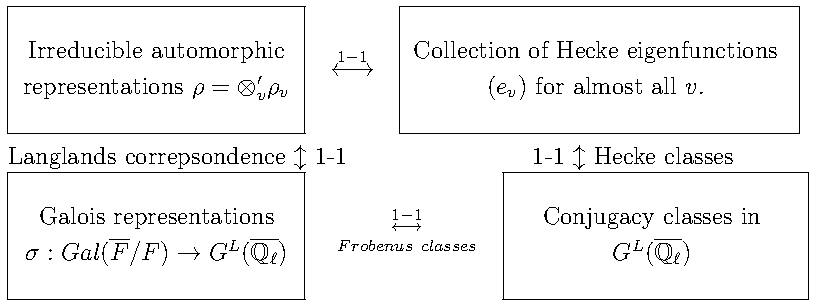
\includegraphics[width=0.6576\paperwidth]{images/L20-p170-correspondence.pdf}\end{figure}
一般连通约化群$G$不具备上述第3、4条性质，第5条所述的唯一性也不能直接推广为任意$G^L$值表示的唯一性。因此，不能为一般约化群照搬第6条所描述的猜想。

虽然无法普遍建立表示之间简单的一一对应，我们仍可在数值层面提出猜想，即通过$L$函数来表述。事实上，$\GL_n$的Langlands猜想可用$L$函数\znote{$L$ 函数把局部数据（$t(\rho_v)$ 与 $\sigma(\operatorname{Fr}[v])$）乘成整体 Euler 乘积，Langlands 猜想的核心正是这些乘积的解析延拓与函数方程：自守侧与 Galois 侧的非分歧 Euler 因子逐处相同，从而两个 $L$ 函数相等。乘积中的 $S$ 必须包含全部分歧地方与无穷地方，否则因子未必收敛；对 $\GL_n$，自守 $L$ 函数的解析性质可由积分表示得到，而 Artin $L$ 函数一侧则来自 Galois 表示。[来源：S. Gelbart, \textit{An elementary introduction to the Langlands program}, Bull. Amer. Math. Soc. 10 (1984) 177--219（本讲参考文献 [G]）。]}重述为下列猜想。
\originalnumber{3}
\begin{conjecture}[Langlands互反猜想]\label{L20S2O3}
设$L/k$为整体域的有限Galois扩张，其Galois群为$\Gal(L/k)$，$\sigma:\Gal(L/k)\to\GL_n(\C)$为不可约表示。则存在$k$上的尖点自守表示$\rho_\sigma$，使
\[L(s,\rho_\sigma)=L(s,\sigma).\]
\end{conjecture}
上述两个$L$函数在非分歧有限地方的Euler因子为
\[L^S(s,\rho)=\prod_{v\notin S}\det\bigl(I-t(\rho_v)q_v^{-s}\bigr)^{-1},\qquad L^S(s,\sigma)=\prod_{v\notin S}\det\bigl(I-\sigma(\operatorname{Fr}[v])q_v^{-s}\bigr)^{-1},\]
其中$S$包含分歧地方及无穷地方。
\sourcepage{171}
这里$t(\rho_v)$为$\rho_v$在$\GL_n(\C)$中的半单共轭类，$q_v$为$v$处剩余域的元素个数。

设$G$为在域$k$上定义的任意连通约化群，$L/k$为充分大的有限Galois扩张，使其上$G$分裂。可定义复约化群$G^L_0$及$\Gal(L/k)$在其上的作用。半直积
\[G^L:=G^L_0\rtimes\Gal(L/k)\]
具有以下性质。
\begin{enumerate}[label=\arabic*.]
\item 若$G$在$k$上分裂，则$G^L_0$为其Langlands对偶群，$G^L$为直积，即$\Gal(L/k)$在$G^L_0$上的作用平凡。
\item 一般而言，若$v$在$L$中非分歧，且$G$在$v$处为非分歧群，选取一个对应的Frobenius元素$\operatorname{Fr}[v]$，则$G(k_v)$的不可约非分歧表示\znote{设 $G$ 在 $F$ 上分裂。$G(F)$ 的不可约光滑表示称为\textbf{未分歧}的，若它有非零的 $G(\OO_F)$-不变向量；此时不变向量空间是一维，表示由它在球面 Hecke 代数上的特征（即 Satake 参数）唯一确定。对 $\GL_n$，未分歧性在 Galois 侧表现为 $\sigma$ 在 $v$ 处未分歧，而 Satake 参数正是 $\sigma(\operatorname{Fr}_v)$ 的半单共轭类，这就是上文第 6 条所说的逐处对应。[来源：J. Bernstein, S. Gelbart (eds.), \textit{An introduction to the Langlands Program}, Birkhäuser 2004, 第 11 章（J. W. Cogdell）（本讲参考文献 [BG]）。]}$\rho_v$与相应的半单Satake参数$t(\rho_v)\in G^L$的$G^L_0$共轭类一一对应，其在$\Gal(L/k)$中的投影为$\operatorname{Fr}[v]$。
\end{enumerate}
$G^L$称为$G$的\textbf{$L$群的Galois形式}\znote{$L$ 群把对偶群与 Galois 作用打包在一起：$G^L=G^L_0\rtimes\Gal(L/k)$。$G$ 分裂时作用平凡，$G^L$ 退化为对偶群；一般情形下，$G(k_v)$ 的未分歧表示对应 $G^L$ 中的共轭类 $t(\rho_v)$，它在 $\Gal(L/k)$ 上的投影必须是 $\operatorname{Fr}[v]$，于是分歧的形状被记录进 $L$ 群的结构。$L$ 同态是与之相容的连续同态，且在 $G^L_0$ 上的限制为代数同态。[来源：J. Bernstein, S. Gelbart (eds.), \textit{An introduction to the Langlands Program}, Birkhäuser 2004, 第 11 章（J. W. Cogdell）（本讲参考文献 [BG]）。]}。$G^L$的表示是同态$r:G^L\to\GL_n(\C)$，要求其在$G^L_0$上的限制为复解析的。两个$L$群$G^L,G'^L$之间的\textbf{$L$同态}是连续同态$h:G^L\to G'^L$，在连通对偶群上的限制为代数同态，并与两群到$\Gal(L/k)$的自然投影相容，如下交换图所示。
\begin{figure}[H]\centering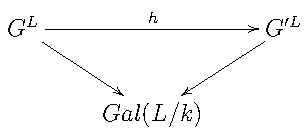
\includegraphics[width=0.2485\paperwidth]{images/L20-p171-Lhom.pdf}\end{figure}
% [Tutor Note: 原书 p171 未写此条，此处按 $L$ 同态的标准定义补足，不改变命题内容。]
于是有以下两个猜想。
\originalnumber{4}
\begin{conjecture}\label{L20S2O4}
设$\rho=\bigotimes'_v\rho_v$为$G$的自守表示，$r$为$G^L$的有限维表示。有Euler乘积
\begin{equation}\tag{2.1}\label{L20eq21}L^S(s,\rho,r)=\prod_{v\notin S}\det\bigl(I-r(t(\rho_v))q_v^{-s}\bigr)^{-1},\end{equation}
其中$S$包括全部分歧地方和无穷地方。这一最初在$s$的某个右半平面定义的$L$函数，可亚纯延拓到整个$\C$，并有联系$L^S(s,\rho,r)$与$L^S(1-s,\widetilde\rho,r)$的函数方程，其中$\widetilde\rho$为逆表示。
\end{conjecture}
\sourcepage{172}
\originalnumber{5}
\begin{conjecture}[关于$L$群的自守形式函子性]\label{L20S2O5}
设$G,G'$为约化群，$f:G^L\to G'^L$为$L$同态。则对$G$的每个自守表示$\rho=\bigotimes'_v\rho_v$，存在$G'$的自守表示$\rho'=\bigotimes'_v\rho'_v$，使在两者及相关群都非分歧的所有地方$v$，$t(\rho'_v)$为包含$f(t(\rho_v))$的$G'^L$共轭类。此外，对$G'^L$的任意有限维表示$r'$，有
\[L(s,\rho',r')=L(s,\rho,r'\circ f).\]
\end{conjecture}
% [Tutor Note: 原书 p172 的猜想 2.5 中，条件写作「$t(\rho'_v)$ 为包含 $t(\rho_v)$ 的共轭类」，漏掉了 $L$ 同态 $f$；译文按 $f(t(\rho_v))$ 处理。]
\originalnumber{6}
\begin{note}[L20S2O6]
\eref{猜想}{L20S2O5}蕴含\eref{猜想}{L20S2O3}与\eref{猜想}{L20S2O4}所期待的结论。取$G'=\GL_n$时，函子性不但给出\eref{猜想}{L20S2O4}的解析性质，还把任意$G$的广义$L$函数研究归约到$\GL_n$的已知理论。取源群$G=\{1\}$、目标群$G'=\GL_n$时，借助两边$L$函数的刚性，就得到\eref{猜想}{L20S2O3}中的互反性结论。
\end{note}
% [Tutor Note: 原书 p172 的注记 2.6 作「If we put $G'=\{1\}$ the trivial group」，应为取源群 $G=\{1\}$、目标群 $G'=\GL_n$；译文按正确写法处理。]
\needspace{5\baselineskip}\section{第20讲参考文献}\label{L20S3}
\begin{references}
\refitem{L20S}{S} I. Satake, \textit{Theory of spherical functions on reductive algebraic groups over p-adic fields}, IHES Publ. Math. 18 (1963) 5--69.
\refitem{L20L}{L} G. Lusztig, \textit{Singularities, character formulas, and a q-analog of weight multiplicities}, \textit{Analysis and topology on singular spaces, II, III} (Luminy, 1981), Ast\'erisque, vol. 101, Soc. Math. France, Paris, 1983, pp. 208--229. MR 737932.
\end{references}
\needspace{4\baselineskip}\textbf{关于Langlands函子性。}
\begin{references}
\refitem{L20BG}{BG} J. Bernstein and S. Gelbart, eds, \textit{An introduction to the Langlands Program}, Birkh\"auser, 2004, Chapter 11 written by J. W. Cogdell.
\refitem{L20G}{G} S. Gelbart, \textit{An elementary introduction to the Langlands program}, Bull. Amer. Math. Soc. 10 (1984) 177--219.
\end{references}

\chapter{几何Satake等价I：球面Hecke代数的范畴化}\label{L21}\lecturedate{2020/04/29}\sourcepage{173}
Satake同构有一个优美的几何版本。本课程最后三讲将围绕这一主题展开，主要遵循Mirković与Vilonen的论文\bref{L21MV}{MV}。

首先回顾，为表述$\GL_n$的几何Langlands对应，我们已经做了哪些工作。
\begin{enumerate}[label=\arabic*.]
\item 选取复数域或有限域上曲线$X$的函数域作为基础域$F$。
\item 找到合适的几何空间$\operatorname{Bun}_X$；其向量丛同构类集合可识别为$\GL_n(F)\backslash\GL_n(\A_F)/K$。
\item 借助Grothendieck的“函数—层”字典，把$\GL_n(F)\backslash\GL_n(\A_F)/K$上的Hecke特征函数替换为$\operatorname{Bun}_X$上的Hecke特征层，也就是相应的反常层。
% [Tutor Note: 原书 p173 作 “perverse sheaves over G”，其中 $G$ 系 $\operatorname{Bun}_X$ 之误（该条讲的是 $\operatorname{Bun}_X$ 上的 Hecke 特征层）；译文按 $\operatorname{Bun}_X$ 处理。]
\item 把Galois表示替换为平展基本群$\widehat\pi_1(X)$的表示。
\item 几何表述为：$\widehat\pi_1(X)$的不可约秩$n$表示对应于$\operatorname{Bun}_X$上的Hecke特征层，如下图所示。
\end{enumerate}
\begin{figure}[H]\centering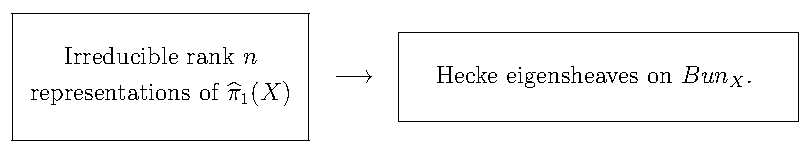
\includegraphics[width=0.6543\paperwidth]{images/L21-p173-correspondence.pdf}\end{figure}
\sourcepage{174}
不过，Satake同构是一个局部命题，因此不需要类似曲线$X$这样的整体对象；即使存在曲线$X$，我们也只考察某一点$x\in X$附近的局部结构。对偶群$G^L$与$G$的\textbf{仿射Grassmannian}\znote{仿射 Grassmannian 是 $\operatorname{Bun}_X$ 的局部模型：在曲线一点附近，向量丛的变形只由 $G(\mathcal K)$ 模 $G(\mathcal O)$ 的等价类刻画。普通 Grassmannian 参数化向量空间的子空间；把向量空间换成形式 Laurent 级数域上的格，就得到仿射版本，名字由此而来。它与对偶群 $G^L$ 一起，在 Satake 对应中分别扮演 $\operatorname{Bun}_X$ 与 $\widehat\pi_1(X)$ 的角色。[来源：nLab "affine Grassmannian"，\url{https://ncatlab.org/nlab/show/affine+Grassmannian}（Last revised 2023-08-15；2026-11-14 访问）。]}将分别扮演类似于$\widehat\pi_1(X)$和$\operatorname{Bun}_X$的角色。

设$G$为有限域$\F_q$或复数域$\C$上的连通分裂约化群。令$\mathcal O=\F_q[[t]]$或$\C[[t]]$，相应地$\mathcal K=\F_q((t))$或$\C((t))$。正环群$G(\mathcal O)$及商$G(\mathcal K)/G(\mathcal O)$具有群概形和ind概形结构；后者记为$\operatorname{Gr}$，即仿射Grassmannian。设$k$为具有有限整体维数的Noether交换含幺环，例如$\C,\Z,\F_q$。以$P_{G(\mathcal O)}(\operatorname{Gr},k)$表示$k$系数的$G(\mathcal O)$等变反常层范畴，以$\operatorname{Rep}G^L_k$表示对偶分裂约化$k$群概形的有限生成$k$表示范畴。几何Satake等价\znote{它把第 19 讲的 Satake 同构在范畴层面提升：不再比较两边的环，而是比较两个张量范畴。易错点：使左边成为对称张量范畴所需的交换约束并非卷积结构自动给出，而是额外的数据，这是本等价最微妙之处。[来源：nLab "geometric Satake equivalence"，\url{https://ncatlab.org/nlab/show/geometric+Satake+equivalence}（Last revised 2024-07-22；2026-11-14 访问）。]}为下列定理。
\originalnumber{1}
\begin{theorem}\label{L21S0O1}
范畴$P_{G(\mathcal O)}(\operatorname{Gr},k)$与$\operatorname{Rep}G^L_k$作为张量范畴等价。
\end{theorem}\idx{几何Satake等价}\idx{仿射Grassmannian}
\section{仿射Grassmannian}\label{L21S1}
为了遵循Mirković–Vilonen的论述并使叙述简明，以下几何基础域始终取$\C$。不过，整个理论的大部分可在整数上建立，见\bref{L21MV}{MV}第14节。若希望了解这里列出的仿射Grassmannian性质的详细证明，可参看\bref{L21BD}{BD}第4.5节。

设$G$为$\C$上的连通约化群。以$\mathcal R$表示Noether交换含幺$\C$代数的范畴。$G$的仿射Grassmannian$\operatorname{Gr}=\operatorname{Gr}_G$是$\C$上的 ind 有限型 ind 概形\znote{ind 概形是概形范畴中的 ind-对象，即按闭嵌入取滤过的正向极限 $\varinjlim_nX_n$。它比有限型概形大得多，正因如此才能在第 3 节用直接极限定义整体的反常层范畴；形式环空间常是 ind 概形而并非概形。对仿射 Grassmannian，$X_n$ 可取第 1 节式 (1.1) 中的有限型闭子概形 $\operatorname{Gr}^n$。[来源：nLab "ind-scheme"，\url{https://ncatlab.org/nlab/show/ind-scheme}（Last revised 2023-11-11；2026-11-14 访问）。]}，代表以下函子$\operatorname{Gr}_G:\mathcal R\to\mathbf{Sets}$：
\[\operatorname{Gr}_G(R)=\left\{(\mathcal P,\alpha)\ \middle|\ \begin{array}{l}\mathcal P\text{ 是 }\Spec R[[t]]\text{ 上的主 }G\text{ 丛},\\\alpha:\mathcal P|_{\Spec R((t))}\xrightarrow{\sim}\mathcal P^0|_{\Spec R((t))}\end{array}\right\}\big/\text{同构},\]
其中$\mathcal P^0=G\times\Spec R[[t]]$为$\Spec R[[t]]$上的平凡$G$丛。
\sourcepage{175}
令$\mathcal K=\C((t))$，$\mathcal O=\C[[t]]$。以下引理解释了为什么$\operatorname{Gr}$是几何框架中$\operatorname{Bun}_X$的局部对应物。
\originalnumber{1}
\begin{lemma}\label{L21S1O1}$G(\mathcal K)/G(\mathcal O)$与$\operatorname{Gr}_G(\C)$之间存在自然双射。\end{lemma}
\begin{proof}
当剩余域为代数闭域时，$\Spec k[[t]]$上的每个$G$丛都可平凡化。因此，$\Spec\mathcal O$上的$G$丛$\mathcal P$可选取平凡化$\beta:\mathcal P\xrightarrow{\sim}\mathcal P^0$。每个$(\mathcal P,\alpha)\in\operatorname{Gr}_G(\C)$便给出$\mathcal P^0|_{\Spec\mathcal K}$的自同构$\alpha\circ\beta^{-1}|_{\Spec\mathcal K}\in G(\mathcal K)$。改变$\beta$仅改变其右侧的$G(\mathcal O)$因子，因而得到唯一确定的右陪集。这就证明了引理。
% [Tutor Note: 原书 p175 证明中作 $\beta^{-1}|_{\Spec\mathcal K}\circ\alpha^{-1}$，但 $\beta^{-1}\circ\alpha^{-1}$ 的余域是 $\mathcal P$ 而非 $\mathcal P^0$，不能视为 $G(\mathcal K)$ 的元素；译文按 $\alpha\circ\beta^{-1}|_{\Spec\mathcal K}$ 处理。]
\end{proof}
\originalnumber{2}
\begin{note}[L21S1O2]
\begin{enumerate}[label=(\arabic*)]
\item 若$G$在$\Z$上定义，则$\operatorname{Gr}_G$也可在$\Z$上定义。
\item 若$F$为非阿基米德局部域，$\OO_F$为其整数环，剩余域为$\F_q$，并给$G$选定合适的光滑连通$\OO_F$模型，则相应局部仿射Grassmannian也满足$G(F)/G(\OO_F)\cong\operatorname{Gr}_G(\F_q)$。
\end{enumerate}
\end{note}
函子$\operatorname{Gr}_G$由ind有限型且ind射影的ind概形代表，是一个不平凡的事实。下面说明其约化结构：$\operatorname{Gr}(\C)$可以写成一族在$\C$上射影、有限型的闭约化子概形的并。

由于可取嵌入$G\hookrightarrow\GL_n$，只需对$\GL_n$说明这一构造。此时$\GL_n(\mathcal O)\cong\operatorname{Aut}(\mathcal O^{\oplus n})$。对正整数$s$，定义有界格的集合
\begin{equation}\tag{1.1}\label{L21eq11}\operatorname{Gr}^{s}:=\{g\mathcal O^{\oplus n}\mid g\in\GL_n(\mathcal K),\ t^s\mathcal O^{\oplus n}\subseteq g\mathcal O^{\oplus n}\subseteq t^{-s}\mathcal O^{\oplus n}\}.\end{equation}
显然$\operatorname{Gr}(\C)=\bigcup_{s\ge0}\operatorname{Gr}^s$。另一方面，$V:=t^{-s}\mathcal O^{\oplus n}/t^s\mathcal O^{\oplus n}\cong\C^{2sn}$，因而有映射
\[\operatorname{Gr}^s\to\operatorname{Gr}(\cdot,V):=\bigsqcup_{0\le m\le2sn}\operatorname{Gr}(m,V),\qquad g\mathcal O^{\oplus n}\longmapsto g\mathcal O^{\oplus n}/t^s\mathcal O^{\oplus n},\]
这里$\operatorname{Gr}(m,V)$为向量空间$V$的通常Grassmannian。该映射把有界格空间的约化结构实现为$\operatorname{Gr}(\cdot,V)$的闭约化子概形，因此它射影且有限型。其像作为点集恰为
\[\operatorname{Gr}(\cdot,V)^t=\{W\subseteq V\mid tW\subseteq W\}.\]

\originalnumber{3}
\begin{note}[L21S1O3]仿射Grassmannian 的 ind 概形本身约化，当且仅当$\operatorname{Hom}(G,\mathbb G_m)=0$，见\bref{L21BD}{BD}的定理4.5.1。\end{note}
Beauville–Laszlo还给出了$\operatorname{Gr}_G$的另一种解释。设$C$为域$k$上的曲线，例如$k=\C$或$\F_q$。固定一个光滑$k$有理点$x\in C$，并选取$x$处的局部参数。
\sourcepage{176}
令$C^*=C\setminus\{x\}$。定义函子$\operatorname{Gr}_{G,x}:\mathcal R\to\mathbf{Sets}$：
\[\operatorname{Gr}_{G,x}(R)=\left\{(\mathcal P,\alpha)\ \middle|\ \begin{array}{l}\mathcal P\text{ 是 }C_R\text{ 上的 }G\text{ 丛},\\\alpha:\mathcal P|_{C^*_R}\xrightarrow{\sim}G\times C^*_R\end{array}\right\}\big/\text{同构}.\]
\originalnumber{4}
\begin{theorem}[Beauville–Laszlo]\label{L21S1O4}$\operatorname{Gr}_{G,x}$与$\operatorname{Gr}_G$同构。\end{theorem}
\section{仿射Grassmannian的胞腔}\label{L21S2}\idx{环群}\idx{半无限轨道}
以下讨论约化ind概形及其经典拓扑。设$Z(G)$为$G$的中心，$Z=Z(G)^0$为中心中包含单位元的连通分支，令$\bar G=G/Z$。则有非典范同构
\begin{equation}\tag{2.1}\label{L21eq21}(\operatorname{Gr}_G)_{\mathrm{red}}\cong\operatorname{Gr}_{\bar G}\times X^\vee(Z),\end{equation}
其中$X^\vee(Z)=\operatorname{Hom}(\C^\times,Z)$。
% [Tutor Note: 原书 p176 的 (2.1) 未标约化，直接写作 $\operatorname{Gr}_G\cong\operatorname{Gr}_{\bar G}\times X^\vee(Z)$；当 $Z\ne1$ 时 $\operatorname{Gr}_G$ 可以非约化，译文按约化结构 $(\operatorname{Gr}_G)_{\mathrm{red}}$ 处理。]

$G(\mathcal K)$也称为$G$的\textbf{环群}\znote{「环群」有拓扑与代数两层含义：拓扑上是自由环空间 $\mathcal LG=\operatorname{Map}(S^1,G)$，可分解为 $G\times\Omega G$（基于环空间），其表示论远比 $G$ 丰富；代数上则指形式 Laurent 级数的点 $G(\mathcal K)$。本讲的中心扩张与 Kac--Moody 代数都属于代数版本。注意代数版本只取形式 Laurent 级数的点，不是拓扑极限。[来源：nLab "loop group"，\url{https://ncatlab.org/nlab/show/loop+group}（Last revised 2026-03-21；2026-11-14 访问）。]}。设$\Gamma\cong\C^\times$为$\operatorname{Aut}(\mathcal K)$中按$t\mapsto st$作用的子群，其中$s\in\Gamma$。$\Gamma$也作用于$G(\mathcal O)$和$G(\mathcal K)$，因而可组成半直积
\[\widetilde G(\mathcal K):=G(\mathcal K)\rtimes\Gamma,\]
其中包含Cartan子群$T\times\Gamma$，$T$为$G$的极大环面。相应的\textbf{仿射Kac–Moody群}$\widehat G(\mathcal K)$为$\widetilde G(\mathcal K)$的一个中心扩张\znote{中心扩张是短正合列 $1\to A\to\widehat G\to G\to1$，且 $A$ 的像落在 $\widehat G$ 的中心。对环群 $G(\mathcal K)$，其中心扩张的 Lie 代数正是下面的 $\widehat{\g}$：扩张的核 $\mathbb G_m$ 对应中心元 $c$，其系数通常称为能级。扩张的存在性依赖 $G$ 上的不变双线性型（Killing 型即可）；换用另一个双线性型相当于把 $c$ 乘上常数，故扩张按该常数分类，这个常数就是能级。[来源：nLab "group extension"，\url{https://ncatlab.org/nlab/show/group+extension}（Last revised 2026-02-23；2026-11-14 访问）。]}：
\[1\to\mathbb G_m\to\widehat G(\mathcal K)\to\widetilde G(\mathcal K)\to1.\]
其Lie代数为Kac--Moody 代数\znote{$\widehat{\g}$ 是最重要的一类 Kac--Moody 代数，即仿射型：它由环代数 $\g((t))$ 添上中心元 $c$ 与导出元 $d$ 得到，可看成环群的切代数加上与量子化（量子异常）有关的修正项；添 $d$ 是为了让 $\delta$ 成为 $\widehat{\mathfrak h}$ 上真正的根，从而得到与有限维情形平行的根空间分解。[来源：nLab "affine Lie algebra"，\url{https://ncatlab.org/nlab/show/affine+Lie+algebra}（Last revised 2024-12-08；2026-11-14 访问）。]}
\[\widehat{\g}=\g((t))\oplus\C c\oplus\C d,\]
Lie括号由下式给出：
\begin{align*}
[x(t),y(t)]&=[x(t),y(t)]_{\g}+\operatorname{Res}_{t=0}\left(\frac{dx(t)}{dt},y(t)\right)dt\,c,\\
[d,x(t)]&=t\frac{dx(t)}{dt},\\
[x(t),c]&=0=[d,c].
\end{align*}
这里$[-,-]_{\g}$为$\g$上的Lie括号在$\g((t))$上的延拓，$(-,-)$为$\g$上的不变双线性型；例如Killing型。
\sourcepage{177}
Cartan子代数为$\widehat{\mathfrak h}=\mathfrak h\oplus\C c\oplus\C d$，其中$\mathfrak h$为$\g$的Cartan子代数。根集合为
\[\widehat\Phi=\{\alpha+m\delta\mid\alpha\in\Phi\cup\{0\},\ m\in\Z\}\setminus\{0\},\]
其中$\delta$为$\widetilde T=T\times\Gamma$的特征标，在$T$上平凡，在$\Gamma$上为恒等特征标。选取$B\supseteq T$，并记其幂幺根基为$N$。$B$中的根就是$G$的正根。$\widehat G(\mathcal K)$的正根集合定义为
\[\widehat\Phi_+=\{\alpha+m\delta\mid\alpha\in\Phi_+,\ m\ge0\}\cup\{\alpha+n\delta\mid\alpha\in\Phi_-\cup\{0\},\ n>0\}.\]
% [Tutor Note: 原书 p177 正根定义中两个集合的哑标都写作 $k$（$k\ge0$ 与 $k>0$），译文分别改用 $m,n$ 以免混淆。]
以$\delta^\vee$表示$\Gamma\hookrightarrow\widetilde T$这一余特征标。

群概形$G(\mathcal O)$以左乘方式作用于$\operatorname{Gr}$，其轨道均为有限维。设$\lambda\in X^\vee(T)$为$T$的余特征标。它在$\mathcal K$值点上给出同态$\lambda_t:\mathcal K^\times\to T(\mathcal K)$。其伴随作用满足
\[\operatorname{Ad}_{\lambda_t(at^m)}(x_\alpha\otimes t^n)=a^{\langle\alpha,\lambda\rangle}x_\alpha\otimes t^{n+m\langle\alpha,\lambda\rangle},\qquad a\in\C^\times,\ m,n\in\Z,\ x_\alpha\in\g_\alpha.\]
% [Tutor Note: 原书 p177 的伴随作用公式右端作 $t^{n+\langle\alpha,\lambda\rangle}$，漏掉了 $at^m$ 中 $t^m$ 贡献的因子；译文按 $t^{n+m\langle\alpha,\lambda\rangle}$ 处理。]
记$t^\lambda=\lambda_t(t)$，并以$L_\lambda=t^\lambda G(\mathcal O)\in\operatorname{Gr}(\C)$表示对应的点。令$\operatorname{Gr}_\lambda$为包含$L_\lambda$的$G(\mathcal O)$轨道。于是$\operatorname{Gr}=\bigcup_{\lambda\in X^\vee}\operatorname{Gr}_\lambda$。设$W$为$T$的Weyl群。由Bruhat分解，$L_{w(\lambda)}$与$L_\lambda$位于同一$G(\mathcal O)$轨道，因此这些轨道由$X^\vee(T)$中的$W$轨道参数化，即
\[\operatorname{Gr}=\bigsqcup_{\lambda\in(X^\vee)^+}\operatorname{Gr}_\lambda.\]
这也称为Cartan分解\znoteplain{这里有两种「分解」，不要混淆：$\operatorname{Gr}=\bigsqcup_\lambda\operatorname{Gr}_\lambda$ 是按 $G(\mathcal O)$ 轨道（按支配余权）的分解，原书 p177 称之为 Cartan 分解（文献中亦用此名，此处按原书用词）；第 2 节末所说的胞腔分解，则是 $G/P_\lambda$ 的 Bruhat 胞腔（$G=\bigsqcup_{w}BwB$）沿纤维丛拉回所得。前者不是胞腔分解：每个 $G(\mathcal O)$ 轨道本身仍是有限维簇；正是这一有限维性使第 2 节能用有限维子簇的极限来刻画 $\operatorname{Gr}$。（上下文推断，无外部依据）}。由环旋转$t\mapsto st$诱导的$\C^\times$作用，其不动点集恰为$\bigsqcup_{\lambda\in(X^\vee)^+}G\cdot L_\lambda$。根据Białynicki–Birula定理，见\bref{L21B}{B}的定理4.1，可进一步得到下列命题。
\originalnumber{1}
\begin{proposition}\label{L21S2O1}
对支配余权$\lambda$，在$t=0$处求值的映射$\operatorname{ev}:G(\mathcal O)\to G$诱导的自然投影$\operatorname{Gr}_\lambda\to G\cdot L_\lambda$为纤维丛，其纤维同构于$\ker(\operatorname{ev})\cdot L_\lambda$。特别地，$\dim\operatorname{Gr}_\lambda=2\langle\kappa,\lambda\rangle$，其中$\kappa$为所有正根之和的一半。
\end{proposition}
注意，$\ker(\operatorname{ev})$为正同余群，其Lie代数为$t\g[[t]]$。选取有序根群坐标后，轨道纤维的坐标由
\[\bigoplus_{\substack{\alpha\in\Phi\\0<m<\langle\alpha,\lambda\rangle}}\g_\alpha\otimes t^m\]
给出，因此
\[\ker(\operatorname{ev})\cdot L_\lambda\cong\C^{\sum_{\alpha\in\Phi,\ \langle\alpha,\lambda\rangle>0}(\langle\alpha,\lambda\rangle-1)}.\]
\sourcepage{178}
令$n_\lambda=\sum_{\alpha\in\Phi,\ \langle\alpha,\lambda\rangle>0}(\langle\alpha,\lambda\rangle-1)$，则$\operatorname{Gr}_\lambda\to G\cdot L_\lambda$为$\C^{n_\lambda}$纤维丛。又$G\cdot L_\lambda\cong G/P_\lambda$，其中$P_\lambda$为$L_\lambda$的稳定子群，是由
\[\Delta_\lambda=\{\alpha\text{ 为单根}\mid\langle\alpha,\lambda\rangle=0\}\]
确定的、与相应标准抛物子群相反的抛物子群；标准抛物子群的定义见\sref{L19S1}。
% [Tutor Note: 原书 p178 称 $P_\lambda$ 为 $\Delta_\lambda$ 确定的 “standard parabolic subgroup”；但按正文 $G(\mathcal O)$ 左乘 $G(\mathcal K)/G(\mathcal O)$ 的约定，$L_\lambda$ 的稳定子是与标准抛物子群相反的抛物子群（例如 $G=\operatorname{SL}_2$、$\lambda$ 正则支配时稳定子为 $B^-$），译文按此处理。]因此
\[\dim G\cdot L_\lambda=|\{\alpha\in\Phi\mid\langle\alpha,\lambda\rangle<0\}|,\]
且
\[\dim\operatorname{Gr}_\lambda=\sum_{\substack{\alpha\in\Phi\\\langle\alpha,\lambda\rangle>0}}\langle\alpha,\lambda\rangle=2\langle\kappa,\lambda\rangle,\]
因为配对为负与为正的根的个数相同。Bruhat分解给出$G/P_\lambda$的胞腔分解，从而也给出每个$G(\mathcal O)\cdot L_\lambda$的胞腔分解。
\originalnumber{2}
\begin{proposition}\label{L21S2O2}
对支配余权$\gamma,\lambda$，$\operatorname{Gr}_\gamma\subseteq\overline{\operatorname{Gr}_\lambda}$当且仅当$\gamma\le\lambda$，即$\lambda-\gamma$为正余根的非负整系数和。
\end{proposition}
\originalnumber{3}
\begin{note}[L21S2O3]
\begin{enumerate}[label=(\arabic*)]
\item 严格来说，Białynicki–Birula定理用于代数簇，而不能直接用于整个ind概形。不过，可以在所需的有限维轨道及适当的有限维部分上应用这一方法。
\item 还存在反向Cartan分解：$\operatorname{Gr}=\bigsqcup_{\lambda\in(X^\vee)^+}\operatorname{Gr}^-_\lambda$，其中$\operatorname{Gr}^-_\lambda=G(\C[t^{-1}])\cdot L_\lambda$。在$t^{-1}=0$处求值诱导投影$\operatorname{Gr}^-_\lambda\to G\cdot L_\lambda$。在非平凡半单情形，纤维为无限维；其在$L_\lambda$处的切空间方向由
\[\mathfrak h\otimes t^{-1}\C[t^{-1}]\ \oplus\!\bigoplus_{\substack{\alpha\in\Phi\\m<\min\{0,\langle\alpha,\lambda\rangle\}}}\g_\alpha\otimes t^m\]
描述。
% [Tutor Note: 原书 p178 的 Remark 2.3(2) 只写出根空间部分 $\bigoplus_{\alpha\in\Phi,\ m<\min\{0,\langle\alpha,\lambda\rangle\}}\g_\alpha\otimes t^m$，略去了环面方向 $\mathfrak h\otimes t^{-1}\C[t^{-1}]$；译文补全了切空间的方向分解。]
\end{enumerate}
\end{note}
对于秩$r$的环面，$T(\mathcal O)\cong(\C[[t]]^\times)^r\cong(\C^\times)^r\times(1+t\C[[t]])^r$。每个余特征标都诱导$\operatorname{Gr}$上的$\C^\times$作用。考虑$2\kappa^\vee$所诱导的作用，不动点集为$\{L_\lambda\mid\lambda\in X^\vee\}$。% [Tutor Note: 原书 p178 作 $T(\mathcal O)\cong(\C[[t]]^\times)^r=(\C^\times)^r$，但 $\C[[t]]^\times\ne\C^\times$（还差主单位部分 $1+t\C[[t]]$）；译文按 $(\C^\times)^r\times(1+t\C[[t]])^r$ 处理。]
相应的吸引集与排斥集为
\[\operatorname{Gr}^{2\kappa^\vee,+}_\gamma=S_\gamma:=N(\mathcal K)\cdot L_\gamma,\qquad\operatorname{Gr}^{2\kappa^\vee,-}_\gamma=T_\gamma:=N^-(\mathcal K)\cdot L_\gamma,\]
其中$N^-$为$N$在Cartan对合下的像。最终得到Iwasawa分解
\[\operatorname{Gr}=\bigsqcup_{\gamma\in X^\vee}S_\gamma,\qquad\operatorname{Gr}=\bigsqcup_{\gamma\in X^\vee}T_\gamma.\]
这些半无限轨道$S_\gamma,T_\gamma$一般既不是有限维，也不是有限余维；但它们与$\overline{\operatorname{Gr}_\lambda}$的交是代数簇。
\originalnumber{4}
\begin{proposition}\label{L21S2O4}
\begin{enumerate}[label=(\arabic*)]
\item $\overline{S_\gamma}=\bigcup_{\nu\le\gamma}S_\nu$。
\item 把$\operatorname{Gr}$嵌入适当的ind射影空间后，$\overline{S_\gamma}$中$S_\gamma$的边界由一个超平面截面给出。
\end{enumerate}
\end{proposition}
为了构造第二条所需的嵌入，先归约到$G$单且单连通的情形，此时$\operatorname{Pic}(\operatorname{Gr})\cong\Z$。
\sourcepage{179}
设$\mathcal L$为$\operatorname{Pic}(\operatorname{Gr})$的丰沛生成元。仿射Kac–Moody群$\widehat G(\mathcal K)$作用于$H^0(\operatorname{Gr},\mathcal L)^\vee$，由此诱导$G(\mathcal K)$等变嵌入
\[\operatorname{Gr}\hookrightarrow\mathbb P\bigl(H^0(\operatorname{Gr},\mathcal L)^\vee\bigr).\]
% [Tutor Note: 原书 p179 写作 $\operatorname{Gr}\hookrightarrow\mathbb P(H^0(\operatorname{Gr},\mathcal L))$；由整体截面的求值映射得到的嵌入应取对偶空间 $\mathbb P(H^0(\operatorname{Gr},\mathcal L)^\vee)$，译文按后者处理。]
\originalnumber{5}
\begin{theorem}\label{L21S2O5}
设$\lambda$为支配余权。
\begin{enumerate}[label=(\arabic*)]
\item $S_\gamma\cap\overline{\operatorname{Gr}_\lambda}$非空，当且仅当$L_\gamma\in\overline{\operatorname{Gr}_\lambda}$；非空时，它纯维，维数为$\langle\kappa,\gamma+\lambda\rangle$。
\item $T_\gamma\cap\overline{\operatorname{Gr}_{-\lambda}}$非空，当且仅当$L_\gamma\in\overline{\operatorname{Gr}_{-\lambda}}$；非空时，它纯维，维数为$\langle\kappa,\lambda-\gamma\rangle$。
\end{enumerate}
\end{theorem}
% [Tutor Note: 原书 p179 定理 2.5(1) 首句的 $S_\gamma\cap\operatorname{Gr}_\lambda$ 漏了上划线（同一句后半作 $S_\gamma\cap\overline{\operatorname{Gr}_\lambda}$，p178 的 Remark 2.3 也只用 $\overline{\operatorname{Gr}_\lambda}$ 的闭包），译文按 $\overline{\operatorname{Gr}_\lambda}$ 处理。]
% [Tutor Note: 原书 p179 定理 2.5(2) 的维数写作 $\langle\kappa,\gamma-\lambda\rangle$；由 $t\mapsto t^{-1}$ 的对称性（$S_\gamma\leftrightarrow T_{-\gamma}$、$\operatorname{Gr}_\lambda\leftrightarrow\operatorname{Gr}_{-\lambda}$）应为 $\langle\kappa,\lambda-\gamma\rangle$，原写法在 $\lambda$ 支配时可为负、不可能是维数；译文按正确写法处理。]
\originalnumber{6}
\begin{note}[L21S2O6]
$L_\gamma\in\overline{\operatorname{Gr}_\lambda}$当且仅当$\gamma$为$G^L(\C)$的最高权$\lambda$不可约表示的一个权。
\end{note}
\originalnumber{7}
\begin{corollary}\label{L21S2O7}
对任意$\lambda\in(X^\vee)^+$及任意$T$不变闭子集$Y\subseteq\overline{\operatorname{Gr}_\lambda}$，有
\[\dim Y\le\max_{L_\gamma\in Y^T}\langle\kappa,\lambda+\gamma\rangle,\]
其中$Y^T$为$Y$的$T$不动点集。
\end{corollary}
\section{仿射Grassmannian上的反常层}\label{L21S3}\idx{权函子}
回忆，在复代数簇$M$上定义反常层时，可以先选取$M$的一个Whitney分层$\mathcal S$。对于ind概形$\operatorname{Gr}$，选取$G(\mathcal O)$轨道给出的分层，即$\operatorname{Gr}=\bigsqcup_{\lambda\in(X^\vee)^+}\operatorname{Gr}_\lambda$。可写成
\[\operatorname{Gr}=\varinjlim_n\operatorname{Gr}^n=\bigcup_{n>0}\operatorname{Gr}^n,\]
其中$\operatorname{Gr}^n$为\eqref{L21eq11}所述的射影约化子概形；对一般$G$，采用相应的$G(\mathcal O)$不变有界部分。令$P_{G(\mathcal O)}(\operatorname{Gr}^n,k)$为$\operatorname{Gr}^n$上的$G(\mathcal O)$等变反常层范畴，定义
\[P_{G(\mathcal O)}(\operatorname{Gr},k):=\varinjlim_nP_{G(\mathcal O)}(\operatorname{Gr}^n,k).\]
这里，对$n\le m$，闭嵌入$\operatorname{Gr}^n\hookrightarrow\operatorname{Gr}^m$的直像诱导全忠实嵌入$P_{G(\mathcal O)}(\operatorname{Gr}^n,k)\hookrightarrow P_{G(\mathcal O)}(\operatorname{Gr}^m,k)$，因此上述直接极限有意义。另以$P_{\mathcal S}(\operatorname{Gr},k)$表示相对于$G(\mathcal O)$轨道可构造、并具有有限维支撑的反常层范畴。
% [Tutor Note: 原书 p179 定义 $P_{\mathcal S}(\operatorname{Gr},k)$ 时只说相对 $G(\mathcal O)$ 轨道可构造，未提有限维支撑；但第 23 讲 p191 的 Remark 1.1 按「按定义 $\mathcal A$ 落在某个 $\operatorname{Gr}^s$ 上」使用该范畴，译文补上「有限维支撑」这一条件。]有以下命题。
\originalnumber{1}
\begin{proposition}\label{L21S3O1}
范畴$P_{G(\mathcal O)}(\operatorname{Gr},k)$与$P_{\mathcal S}(\operatorname{Gr},k)$自然等价。
\end{proposition}
\sourcepage{180}
下面列出$\operatorname{Gr}$上反常层的一些性质，不给出证明；证明可见\bref{L21MV}{MV}。
\begin{itemize}
\item 对任意$\mathcal A\in P_{G(\mathcal O)}(\operatorname{Gr},k)$，有典范同构
\[H_c^l(S_\gamma,\mathcal A)\xrightarrow{\sim}H_{T_\gamma}^l(\operatorname{Gr},\mathcal A),\]
且当$l\ne2\langle\kappa,\gamma\rangle$时，两边均为零。这里$H_Y^l(-)$为支集在$Y$中的上同调。
\item 函子$F_\gamma:P_{G(\mathcal O)}(\operatorname{Gr},k)\to\{\text{有限生成 }k\text{ 模}\}$，定义为
\[F_\gamma:=H_c^{2\langle\kappa,\gamma\rangle}(S_\gamma,-)=H_{T_\gamma}^{2\langle\kappa,\gamma\rangle}(\operatorname{Gr},-),\]
是正合函子。
\item 存在自然的函子同构
\[H^*\cong F:=\bigoplus_{\gamma\in X^\vee}H_c^{2\langle\kappa,\gamma\rangle}(S_\gamma,-):P_{G(\mathcal O)}(\operatorname{Gr},k)\to\{\text{有限生成 }k\text{ 模}\}.\]
此外，在相应的共轭识别下，权函子$F_\gamma$及这一同构不依赖于$T\subseteq B$的选择。因此，整体上同调函子$H^*$忠实且正合。
\item 对有限生成$k$模$M$，分别以$\mathcal I_!(\lambda,M),\mathcal I_*(\lambda,M),\mathcal I_{!*}(\lambda,M)$表示反常层
\[{}^pj_!(M[\dim\operatorname{Gr}_\lambda]),\qquad{}^pj_*(M[\dim\operatorname{Gr}_\lambda]),\qquad j_{!*}(M[\dim\operatorname{Gr}_\lambda]),\]
其中$j:\operatorname{Gr}_\lambda\to\operatorname{Gr}$为包含映射；参看\eqref{L13eq22}。则有典范识别
\[F_\gamma[\mathcal I_!(\lambda,k)]\cong k[\operatorname{Irr}(\overline{\operatorname{Gr}_\lambda}\cap S_\gamma)]\cong F_\gamma[\mathcal I_*(\lambda,k)].\]
这里$k[\operatorname{Irr}(\overline{\operatorname{Gr}_\lambda}\cap S_\gamma)]$为由$\overline{\operatorname{Gr}_\lambda}\cap S_\gamma$的不可约分支生成的自由$k$模。
\end{itemize}
\needspace{5\baselineskip}\section{第21讲参考文献}\label{L21S4}
\begin{references}
\refitem{L21MV}{MV} I. Mirkovi\'c and K. Vilonen, \textit{Geometric Langlands duality and representations of algebraic groups over commutative rings}, Annals of Mathematics, 166 (2007), 95--143.
\sourcepage{181}
\refitem{L21BD}{BD} A. Beilinson and V. Drinfeld, \textit{Quantization of Hitchin integrable system and Hecke eigensheaves}, available at \url{http://math.uchicago.edu/~drinfeld/langlands/QuantizationHitchin.pdf}.
\end{references}
\needspace{4\baselineskip}\textbf{关于Białynicki–Birula定理。}
\begin{references}
\refitem{L21B}{B} A. Bia\l ynicki-Birula, \textit{Some theorems on actions of algebraic groups}, Ann. of Math. 98 (1973), 480--497.
\end{references}

\chapter{几何Satake等价II：等变反常层范畴的张量结构}\label{L22}\lecturedate{2020/05/06}\sourcepage{182}
设$k=\C$；关于$k$为一般交换环的情形，参见\bref{L22MV}{MV}。设$G$为分裂约化群，分别记$\mathcal K=k((t))$、$\mathcal O=k[[t]]$。仿射Grassmannian的点集可识别为$G(\mathcal K)/G(\mathcal O)$。

如\lref{L21}所定义，$P_{G(\mathcal O)}(\operatorname{Gr},k)$为仿射Grassmannian上$k$系数的$G(\mathcal O)$等变反常层范畴。回忆，$\operatorname{Gr}$通常为无限维，但它具有由有限维$G(\mathcal O)$轨道组成的分层$\mathcal S$：
\begin{equation}\tag{0.1}\label{L22eq01}\operatorname{Gr}=\bigsqcup_{\lambda\in(X^\vee)^+}\operatorname{Gr}_\lambda,\qquad\operatorname{Gr}_\lambda=G(\mathcal O)\cdot L_\lambda.\end{equation}
这里$\dim\operatorname{Gr}_\lambda=2\langle\kappa,\lambda\rangle$，$\kappa$为$G$的正根之和的一半。令$P_{\mathcal S}(\operatorname{Gr},k)$为相对于这些轨道可构造、具有有限维支撑的反常层范畴。由\eref{命题}{L21S3O1}，有以下结果。
\originalnumber{1}
\begin{proposition}\label{L22S0O1}范畴$P_{G(\mathcal O)}(\operatorname{Gr},k)$与$P_{\mathcal S}(\operatorname{Gr},k)$自然等价。\end{proposition}
\eqref{L22eq01}是约化群Cartan分解的对应物。还有Iwasawa分解的对应物：
\begin{equation}\tag{0.2}\label{L22eq02}\operatorname{Gr}=\bigsqcup_{\gamma\in X^\vee}S_\gamma,\end{equation}
其中$S_\gamma=N(\mathcal K)\cdot L_\gamma$，$N$为固定Borel子群$B$的幂幺根基。
\sourcepage{183}
以$D_{G(\mathcal O)}(\operatorname{Gr},k)$表示$\operatorname{Gr}$上具有有限维支撑的$G(\mathcal O)$等变可构造$k$层的有界导出范畴。由\lref{L21}末列出的性质，得到以下反常性判据。
\originalnumber{2}
\begin{lemma}\label{L22S0O2}对$\mathcal A\in D_{G(\mathcal O)}(\operatorname{Gr},k)$，下列两条等价：
\begin{enumerate}[label=(\roman*)]
\item $\mathcal A$为反常层。
\item 对所有$\gamma\in X^\vee$，$H_c^*(S_\gamma,\mathcal A)$只可能在次数$2\langle\kappa,\gamma\rangle$非零。
\end{enumerate}
\end{lemma}
\begin{proof}
由\lref{L21}末的性质，对反常层$\mathcal P$，$H_c^m(S_\gamma,\mathcal P)\ne0$蕴含$m=2\langle\kappa,\gamma\rangle$。对任意$\mathcal A$，以${}^pH^j(\mathcal A)$表示其第$j$个反常上同调。$\mathcal A$反常当且仅当所有$j\ne0$时${}^pH^j(\mathcal A)=0$。

由反常上同调的谱序列及上述消失性，得到自然同构
\[H_c^{2\langle\kappa,\gamma\rangle}(S_\gamma,{}^pH^j(\mathcal A))\cong H_c^{2\langle\kappa,\gamma\rangle+j}(S_\gamma,\mathcal A).\]
因此
\begin{align*}
\text{(i)}&\Longleftrightarrow{}^pH^j(\mathcal A)=0\quad(j\ne0)\\
&\Longleftrightarrow H_c^{2\langle\kappa,\gamma\rangle}(S_\gamma,{}^pH^j(\mathcal A))=0\quad(j\ne0,\ \gamma\in X^\vee)\\
&\Longleftrightarrow H_c^{2\langle\kappa,\gamma\rangle+j}(S_\gamma,\mathcal A)=0\quad(j\ne0,\ \gamma\in X^\vee)\\
&\Longleftrightarrow\text{(ii)}.
\end{align*}
\end{proof}
\section{卷积积}\label{L22S1}\idx{反常层的卷积}
在Satake同构的几何表述中，$P_{G(\mathcal O)}(\operatorname{Gr},k)$替代Hecke代数，因此需要在对象上定义对应于交换代数乘法的运算，即为反常层$\mathcal A_1,\mathcal A_2$定义\textbf{卷积积}\znote{卷积积是 Hecke 代数乘法的几何化。在 Hecke 代数中，双陪集上的紧支撑函数按卷积 $(f_1*f_2)(g)=\int f_1(h)f_2(h^{-1}g)\,dh$ 相乘；几何版把函数换成反常层，用图 $\operatorname{Gr}\times\operatorname{Gr}\leftarrow G(\mathcal K)\times\operatorname{Gr}\rightarrow G(\mathcal K)\times^{G(\mathcal O)}\operatorname{Gr}\rightarrow\operatorname{Gr}$ 上的拉回与真推前代替积分。易错点：两个步骤都只在层上操作，卷积不能逐点定义；需要先验证所得层反常，这正是命题 1.3 的内容。[来源：nLab \textquotedbl geometric Satake equivalence\textquotedbl，\url{https://ncatlab.org/nlab/show/geometric+Satake+equivalence}（Last revised 2024-07-22；2026-11-14 访问）。]}$\mathcal A_1*\mathcal A_2$。
\sourcepage{184}
考虑下列映射图：
\begin{figure}[H]\centering\begin{equation}\tag{1.1}\label{L22eq11}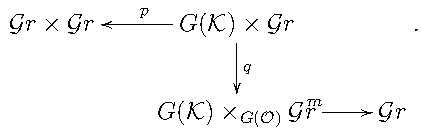
\includegraphics[width=0.3404\paperwidth]{images/L22-p184-convolution.pdf}\end{equation}\end{figure}
这里$G(\mathcal K)\times^{G(\mathcal O)}\operatorname{Gr}$为$G(\mathcal K)\times\operatorname{Gr}$关于$G(\mathcal O)$作用的商，该作用在第一因子为右乘逆元，在第二因子为左乘。\eqref{L22eq11}中$p=p_G\times\operatorname{id}_{\operatorname{Gr}}$，其中$p_G:G(\mathcal K)\to\operatorname{Gr}$为商映射；$q$为上述对角作用的商映射；$m$为乘法映射。定义
\begin{equation}\tag{1.2}\label{L22eq12}\mathcal A_1*\mathcal A_2:=Rm_*\widetilde{\mathcal A},\qquad q^*\widetilde{\mathcal A}=p^*(\mathcal A_1\boxtimes\mathcal A_2).\end{equation}
也可以说，$\widetilde{\mathcal A}$是$p^*(\mathcal A_1\boxtimes\mathcal A_2)$下降到$G(\mathcal K)\times^{G(\mathcal O)}\operatorname{Gr}$后得到的层。注意，$\mathcal A_1,\mathcal A_2$都$G(\mathcal O)$等变，因此$p^*(\mathcal A_1\boxtimes\mathcal A_2)$为$G(\mathcal O)\times G(\mathcal O)$等变层\znote{等变层是带 $G$ 作用的空间 $X$ 上的层 $\mathcal F$，附带同构 $\alpha:a^*\mathcal F\cong\operatorname{pr}^*\mathcal F$（$a:G\times X\to X$ 为作用映射），并要求 $\alpha$ 在结合律意义下满足余圈条件；等价的说法是 $X/G$（或商叠）上的层。易错点：等变结构是附加数据而非层的性质，同一个底层的层可以带不同的等变结构；只有当作用自由时，下降才唯一地把等变层等同于商上的层。[来源：nLab \textquotedbl equivariant sheaf\textquotedbl，\url{https://ncatlab.org/nlab/show/equivariant+sheaf}（Last revised 2024-12-24；2026-11-14 访问）。]}：第一群在$G(\mathcal K)$因子上左乘，第二群按$q$所商掉的对角作用（$G(\mathcal K)$上右乘逆元、$\operatorname{Gr}$上左乘）作用。由于第二群的作用自由，这个等变层唯一地下降到商空间。

赋予$G(\mathcal K)\times^{G(\mathcal O)}\operatorname{Gr}$分层$\mathcal T$，其层为
\begin{equation}\tag{1.3}\label{L22eq13}\widetilde{\operatorname{Gr}}_{\lambda,\gamma}:=p_G^{-1}(\operatorname{Gr}_\lambda)\times^{G(\mathcal O)}\operatorname{Gr}_\gamma.\end{equation}
注意，$\dim\widetilde{\operatorname{Gr}}_{\lambda,\gamma}=2\langle\kappa,\lambda+\gamma\rangle$。
\originalnumber{1}
\begin{lemma}\label{L22S1O1}若$\mathcal A_1,\mathcal A_2$反常，则$\widetilde{\mathcal A}$相对于分层$\mathcal T$反常。\end{lemma}
\begin{proof}
按定义，只需在每个$\widetilde{\operatorname{Gr}}_{\lambda,\gamma}$上检查支撑与余支撑条件。记其包含映射为$i_{\lambda,\gamma}$，$d_{\lambda,\gamma}=2\langle\kappa,\lambda+\gamma\rangle$，则条件为
\[\begin{cases}\mathcal H^j(i_{\lambda,\gamma}^*\widetilde{\mathcal A})=0,&j>-d_{\lambda,\gamma},\\\mathcal H^j(i_{\lambda,\gamma}^!\widetilde{\mathcal A})=0,&j<-d_{\lambda,\gamma}.\end{cases}\]
在$p$与$q$的局部平凡化中，这等价于$\mathcal A_1\boxtimes\mathcal A_2$在$\operatorname{Gr}_\lambda\times\operatorname{Gr}_\gamma$上的同样两个条件：
\[\begin{cases}\mathcal H^j(i_{\operatorname{Gr}_\lambda\times\operatorname{Gr}_\gamma}^*(\mathcal A_1\boxtimes\mathcal A_2))=0,&j>-d_{\lambda,\gamma},\\\mathcal H^j(i_{\operatorname{Gr}_\lambda\times\operatorname{Gr}_\gamma}^!(\mathcal A_1\boxtimes\mathcal A_2))=0,&j<-d_{\lambda,\gamma}.\end{cases}\]
% [Tutor Note: 原书 p184 证明中第二个条件作 $\mathcal H^j_c(\widetilde{\mathcal A}|_{\widetilde{\operatorname{Gr}}_{\lambda,\gamma}})=0,\ \forall j<2\langle\kappa,\lambda+\gamma\rangle$；按中围反常性（即第 21 讲末所列两条消失性质）应为 $\mathcal H^j(i_{\lambda,\gamma}^!\widetilde{\mathcal A})=0,\ \forall j<-2\langle\kappa,\lambda+\gamma\rangle$，译文按标准写法处理。]
\sourcepage{185}
所以只需证明导出外张量积$\mathcal A_1\boxtimes^L\mathcal A_2$相对于$\operatorname{Gr}\times\operatorname{Gr}$上的分层$\mathcal S\times\mathcal S$反常。由\eref{命题}{L22S0O1}与\eref{引理}{L22S0O2}的乘积版本，只需证明
\[H_c^n(S_\gamma\times S_\nu,\mathcal A_1\boxtimes\mathcal A_2)=0,\qquad n\ne2\langle\kappa,\gamma+\nu\rangle.\]
这由Künneth公式
\[H_c^n(S_\gamma\times S_\nu,\mathcal A_1\boxtimes\mathcal A_2)\cong\bigoplus_{n_1+n_2=n}H_c^{n_1}(S_\gamma,\mathcal A_1)\otimes H_c^{n_2}(S_\nu,\mathcal A_2),\]
以及$H_c^n(S_\eta,\mathcal A_i)=0$，$i=1,2$、$n\ne2\langle\kappa,\eta\rangle$，立即得到。
\end{proof}
\originalnumber{2}
\begin{note}[L22S1O2]
一般而言，若$k$不是域，则\eqref{L22eq12}中$\widetilde{\mathcal A}$的定义应改为
\[q^*\widetilde{\mathcal A}=p^*\bigl({}^pH^0(\mathcal A_1\boxtimes^L\mathcal A_2)\bigr).\]
\end{note}
\originalnumber{3}
\begin{proposition}\label{L22S1O3}若$\mathcal A_1,\mathcal A_2$反常，则其卷积积$\mathcal A_1*\mathcal A_2$反常。\end{proposition}
为了证明这一命题，先介绍\textbf{分层半小映射}\znote{半小映射的直觉是：目标层 $T_2$ 上纤维的维数受源层 $\overline{T_1}$ 的余维控制，即 $\dim(f^{-1}(x)\cap\overline{T_1})\le\frac12(\dim\overline{T_1}-\dim T_2)$。它等价于 $\dim(X\times_YX)\le\dim X$，也等价于 $\operatorname{codim}_Y\{y:\dim f^{-1}(y)\ge r\}\ge2r$（命题 1.5）。易错点：条件必须用闭包 $\overline{T_1}$（开层本身不闭），且要求 $f|_{\overline{T_1}}$ 真，否则维数估计失去意义。半小映射的分解定理是本讲把卷积层拆成 IC 层直和的关键。[来源：de Cataldo--Migliorini, \textit{The decomposition theorem, perverse sheaves and the topology of algebraic maps}, \S4.2（本讲参考文献）。]}。设$(Y_1,\mathcal T_1)$、$(Y_2,\mathcal T_2)$为分层复空间。
\begin{definition*}
若每个$T_1\in\mathcal T_1$的像$f(T_1)$都是$\mathcal T_2$中若干层的并，并且对每个$T_2\in\mathcal T_2$，$f^{-1}(T_2)\to T_2$为拓扑局部平凡纤维化，则称$f:Y_1\to Y_2$为相对于这两个分层的\textbf{分层映射}。若还满足以下条件，则称其为\textbf{分层半小映射}：
\begin{enumerate}[label=\arabic*.]
\item 对每个$T_1\in\mathcal T_1$，$f|_{\overline{T_1}}$为真映射；
\item 对任意$T_1\in\mathcal T_1$与满足$T_2\subseteq f(\overline{T_1})$的任意$T_2\in\mathcal T_2$，以及对$T_2$中任意一点$x$，有
\[\dim\bigl(f^{-1}(x)\cap\overline{T_1}\bigr)\le\frac12\bigl(\dim\overline{T_1}-\dim T_2\bigr).\]
\end{enumerate}
由局部平凡性，在$T_2$内任取一点的结果相同。
\end{definition*}\idx{半小映射}
% [Tutor Note: 原书 p185 半小映射条件 2 的不等式右端作 $\frac12(\dim f(\overline{T_1})-\dim T_2)$，其中的像维数应为源层维数 $\frac12(\dim\overline{T_1}-\dim T_2)$，否则爆破等标准例子不满足该条件；译文按后者处理。]
\sourcepage{186}
\begin{definition*}
若存在非空的开稠密分层子集$W\subseteq Y_1$，满足以下条件，则称$f$为\textbf{分层小映射}：
\begin{enumerate}[label=\arabic*.]
\item 对每个$T_1\in\mathcal T_1$，$f|_{\overline{T_1}}$为真映射；
\item $f|_W:W\to f(W)$有限，并且$W=f^{-1}(f(W))$，其中$f(W)$为目标中的开稠密分层部分；
\item 对任意$T_1\in\mathcal T_1$与满足$T_2\subseteq f(\overline{T_1})\setminus f(W)$的任意$T_2\in\mathcal T_2$，以及对$T_2$中任意一点$x$，有
\[\dim\bigl(f^{-1}(x)\cap\overline{T_1}\bigr)<\frac12\bigl(\dim\overline{T_1}-\dim T_2\bigr).\]
\end{enumerate}
\end{definition*}\idx{小映射}
% [Tutor Note: 原书 p186 小映射定义先引入开稠密分层子集 $U\subset Y_1$，条件 2、3 中却改记为 $W$（$U,W$ 混用）；译文统一记为 $W$。]
\originalnumber{4}
\begin{lemma}\label{L22S1O4}
若$f$为分层半小映射，则对任意$\mathcal A\in P_{\mathcal T_1}(Y_1,k)$，$Rf_*\mathcal A\in P_{\mathcal T_2}(Y_2,k)$。若$f$为分层小映射，$W$如上，$\mathcal A$为$W$上的反常层，则
\[Rf_*j_{!*}\mathcal A\cong\widetilde j_{!*}(f|_W)_*\mathcal A,\]
其中$j:W\hookrightarrow Y_1$、$\widetilde j:f(W)\hookrightarrow Y_2$为开包含映射，$j_{!*}$、$\widetilde j_{!*}$为反常中间延拓，见\sref{L13S3}。
\end{lemma}
该引理可由直接的维数估计得到；在下述分解定理适用的情形，也可结合\eref{定理}{L22S1O8}与\eref{定理}{L13S3O4}理解这一结论。

下面暂时讨论一般的半小映射。更详细的内容可见\bref{L22dCM}{dCM}第4.2节。
\originalnumber{5}
\begin{proposition}\label{L22S1O5}
设$X$为连通非奇异$n$维簇，$f:X\to Y$为真满态射。设$Y=\bigsqcup_k S_k$为适合$f$的分层，即$f^{-1}(S_k)\to S_k$拓扑局部平凡。取$y_k\in S_k$，令$d_k=\dim f^{-1}(y_k)=\dim f^{-1}(S_k)-\dim S_k$。以下条件等价：
\begin{enumerate}[label=\arabic*.]
\item $Rf_*\Q_X[n]$为$Y$上的反常层；
\item $\dim(X\times_YX)\le n$；
\item 对每个层$S_k$，$\dim S_k+2d_k\le\dim X$；
\item 对任意$r\ge1$，$\operatorname{codim}_Y\{y\in Y\mid\dim f^{-1}(y)\ge r\}\ge2r$。
\end{enumerate}
\end{proposition}
\sourcepage{187}
满足\eref{命题}{L22S1O5}中任一等价条件的真满态射称为\textbf{半小映射}。若$\dim S_k+2d_k=\dim X$，则称层$S_k$为\textbf{相关层}。还有以下小映射的定义。
\originalnumber{6}
\begin{definition}\label{L22S1O6}
簇之间的真满态射$f:X\to Y$称为\textbf{小映射}，若其满足以下任一等价条件：
\begin{enumerate}[label=\arabic*.]
\item 存在开稠密子集$U\subseteq Y$，使$f^{-1}(U)\to U$有限，并且
\[\dim\bigl((X\times_YX)\setminus(f^{-1}(U)\times_Uf^{-1}(U))\bigr)<\dim X;\]
\item 对任意$r\ge1$，$\operatorname{codim}_Y\{y\in Y\mid\dim f^{-1}(y)\ge r\}>2r$；
\item 每个层都满足$\dim S_k+2d_k\le\dim X$，而且每个在$Y$中不稠密的层都不是相关层，即满足严格不等式$\dim S_k+2d_k<\dim X$。
\end{enumerate}
特别地，小映射都是半小映射。
\end{definition}
% [Tutor Note: 原书 p187 定义 1.6 条件 1 作 $\dim(X\times_YX-\Delta_X)<\dim X$；它与条件 2、3 并不等价（取有限二重覆叠即得反例：小映射成立而条件 1 不成立），译文按 de Cataldo--Migliorini 的标准表述处理。]
\originalnumber{7}
\begin{note}[L22S1O7]半小映射在一般点上有限，反之不成立。例如，$\C^3$中一点的爆破。\end{note}
回忆，$IC_X^\bullet\mathbb V[n]$为$X$上的反常层，称为局部系统$\mathbb V$的反常延拓，见\sref{L13S3}。这种形式的反常层也称为\textbf{IC层}。由\eref{定理}{L13S3O4}，它们是构成$\operatorname{Perv}(X)$中对象的基本组成部分。
\originalnumber{8}
\begin{theorem}\label{L22S1O8}
\begin{enumerate}[label=(\arabic*)]
\item 若$f:X\to Y$为小映射，且在一般点的次数为$1$，则
\[Rf_!IC_X^\bullet\Q[n]\cong IC_Y^\bullet\Q[n],\qquad n=\dim X=\dim Y.\]
特别地，$\operatorname{IH}^j(Y)\cong\operatorname{IH}^j(X)$，其中$\operatorname{IH}^j(Y)$为第$j$个交上同调，即未平移交复形的超上同调$\mathbb H^j(Y,IC_Y^\bullet\Q)$。
\item 若$f:X\to Y$为小映射，$\mathbb V$为源的光滑稠密部分上的局部系统，则
\[Rf_*(IC_X^\bullet\mathbb V[n])\cong IC_Y^\bullet((f|_U)_*\mathbb V)[n],\]
其中$U$取为$f$有限且局部系统定义的适当稠密部分。
\item \textbf{半小映射的分解定理。}对兼容分层的半小映射，$Rf_*(IC_X^\bullet\mathbb V[n])$为反常层。特别地，当$X$光滑且系数为$\Q$时，
\[Rf_*\Q_X[n]\cong\bigoplus_{S_k\text{ 相关}}IC_{\overline{S_k}}^\bullet\mathbb V_k[n-2d_k],\]
其中$\mathbb V_k$为相关层上纤维最高维上同调给出的局部系统。
\end{enumerate}
\end{theorem}\idx{分解定理}\idx{交上同调}
现在回到乘法映射$m:G(\mathcal K)\times^{G(\mathcal O)}\operatorname{Gr}\to\operatorname{Gr}$。源的分层为$\mathcal T=\{\widetilde{\operatorname{Gr}}_{\lambda,\gamma}\}$，其层由\eqref{L22eq13}定义；目标的分层为$\mathcal S=\{\operatorname{Gr}_\lambda\}$。
\sourcepage{188}
\originalnumber{9}
\begin{lemma}\label{L22S1O9}乘法映射$m$相对于上述分层为分层半小映射。\end{lemma}
\begin{proof}
首先，$m(\widetilde{\operatorname{Gr}}_{\lambda,\gamma})$为若干$G(\mathcal O)$轨道的并，包含$\bigcup_{w\in W}\operatorname{Gr}_{\lambda+w(\gamma)}$，并以$\operatorname{Gr}_{\lambda+\gamma}$为稠密轨道。回忆
\[\overline{\operatorname{Gr}_\lambda}=\bigsqcup_{\substack{\nu\in(X^\vee)^+\\\nu\le\lambda}}\operatorname{Gr}_\nu.\]
因此
\[\overline{\widetilde{\operatorname{Gr}}_{\lambda,\gamma}}=\bigsqcup_{\substack{\nu,\theta\in(X^\vee)^+\\\nu\le\lambda,\ \theta\le\gamma}}\widetilde{\operatorname{Gr}}_{\nu,\theta}.\]
更精确地，$\operatorname{Gr}_\xi\subseteq m\bigl(\overline{\widetilde{\operatorname{Gr}}_{\lambda,\gamma}}\bigr)$当且仅当存在$w_1,w_2\in W$及$0\le\lambda'\le\lambda$、$0\le\gamma'\le\gamma$使$w_1(\xi)=\lambda'+w_2(\gamma')$。乘法在这一闭有界卷积空间上的像为$\overline{\operatorname{Gr}_{\lambda+\gamma}}$。它是射影的有界空间，因此$m|_{\overline{\widetilde{\operatorname{Gr}}_{\lambda,\gamma}}}$为真映射。

映射
\[m^{-1}(\operatorname{Gr}_\xi)\xrightarrow{(p_G,m)}\operatorname{Gr}\times\operatorname{Gr}_\xi,\qquad[g,hG(\mathcal O)]\longmapsto(gG(\mathcal O),ghG(\mathcal O))\]
为同构，其逆映射把$(gG(\mathcal O),zG(\mathcal O))$送到$[g,g^{-1}zG(\mathcal O)]$。从而$m$在各目标轨道上为局部平凡纤维化；同样利用等变性，有限维分层部分也局部平凡，所以$m$为分层映射。

接下来只需检查维数条件。对支配余权$\xi$，取同一轨道中的反支配点$L_{w_0\xi}\in\operatorname{Gr}_\xi$，其中$w_0$为最长Weyl群元。我们需要证明
\begin{equation}\tag{1.4}\label{L22eq14}
\dim\bigl(m^{-1}(L_{w_0\xi})\cap\overline{\widetilde{\operatorname{Gr}}_{\lambda,\gamma}}\bigr)\le\tfrac12\bigl(2\langle\kappa,\lambda+\gamma\rangle-\dim\operatorname{Gr}_\xi\bigr)=\langle\kappa,\lambda+\gamma-\xi\rangle.
\end{equation}
$G$的常数环面$T\cong(k^\times)^r$通过左乘$G(\mathcal K)$因子作用于卷积空间。由于$T\subseteq T(\mathcal O)\subseteq G(\mathcal O)$，所有$\operatorname{Gr}_\lambda$及$\overline{\widetilde{\operatorname{Gr}}_{\lambda,\gamma}}$都$T$不变。另一方面，$L_{w_0\xi}$为$T$不动点。因此，\eqref{L22eq14}左端的纤维为$T$不变闭子集。它在同构$(p_G,m)$下的像位于$\operatorname{Gr}\times\{L_{w_0\xi}\}\cong\operatorname{Gr}$中，记为$\widehat{\operatorname{Gr}}^\xi_{\lambda,\gamma}$。显然
\[\widehat{\operatorname{Gr}}^\xi_{\lambda,\gamma}\subseteq\overline{\operatorname{Gr}_\lambda}.\]
我们用\eref{推论}{L21S2O7}来估计其维数。该纤维的$T$不动点可写成$[t^\eta,t^\beta G(\mathcal O)]$，其中
\[L_\eta\in\overline{\operatorname{Gr}_\lambda},\qquad L_\beta\in\overline{\operatorname{Gr}_\gamma},\qquad\eta+\beta=w_0\xi.\]
$\widehat{\operatorname{Gr}}^\xi_{\lambda,\gamma}$的不动点为满足上述条件的$L_\eta$。由\eref{推论}{L21S2O7}及\eref{笔记}{L21S2O6}，得到
\begin{align*}
\dim\widehat{\operatorname{Gr}}^\xi_{\lambda,\gamma}
&\le\max_{L_\eta\in(\widehat{\operatorname{Gr}}^\xi_{\lambda,\gamma})^T}\langle\kappa,\lambda+\eta\rangle\\
&=\max_{\beta}\langle\kappa,\lambda+w_0\xi-\beta\rangle\\
&\le\langle\kappa,\lambda+\gamma-\xi\rangle.
\end{align*}
最后一步用了$\langle\kappa,w_0\xi\rangle=-\langle\kappa,\xi\rangle$，以及最高权$\gamma$表示的任意权$\beta$都满足$\langle\kappa,\beta\rangle\ge-\langle\kappa,\gamma\rangle$。
\sourcepage{189}
由于$(p_G,m)$为同构，这就证明了\eqref{L22eq14}。
\end{proof}

还可用另一种方式定义$\mathcal A_1*\mathcal A_2$。先在$G(\mathcal K)$上定义一个$G(\mathcal O)\times G(\mathcal O)$等变层
\[\widehat{\mathcal A_1*\mathcal A_2}:=R\widehat m_*\mathcal D,\]
其中$\widehat m:G(\mathcal K)\times^{G(\mathcal O)}G(\mathcal K)\to G(\mathcal K)$为乘法，$\mathcal D$由下降条件
\[\widehat q^*\mathcal D=p_G^*\mathcal A_1\boxtimes p_G^*\mathcal A_2\]
定义，$\widehat q:G(\mathcal K)\times G(\mathcal K)\to G(\mathcal K)\times^{G(\mathcal O)}G(\mathcal K)$为商映射。于是$\mathcal A_1*\mathcal A_2$是$\widehat{\mathcal A_1*\mathcal A_2}$唯一地下降到$\operatorname{Gr}$后得到的层。

从这一角度，可以看出卷积积的结合性。考虑下图：
\begin{figure}[H]\centering\begin{equation}\tag{1.5}\label{L22eq15}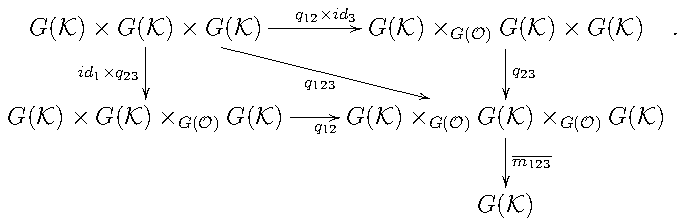
\includegraphics[width=0.5556\paperwidth]{images/L22-p189-associativity.pdf}\end{equation}\end{figure}
$G(\mathcal K)^3$上的$p_G^*\mathcal A_1\boxtimes p_G^*\mathcal A_2\boxtimes p_G^*\mathcal A_3$唯一地下降到
\[G(\mathcal K)\times^{G(\mathcal O)}G(\mathcal K)\times^{G(\mathcal O)}G(\mathcal K),\]
记下降层为$\mathcal D_3$。由\eqref{L22eq15}的交换图，
\[p_G^*((\mathcal A_1*\mathcal A_2)*\mathcal A_3)\cong p_G^*(\mathcal A_1*(\mathcal A_2*\mathcal A_3))\cong Rm_{123*}\mathcal D_3.\]
因此得到以下命题。
\originalnumber{10}
\begin{proposition}\label{L22S1O10}阿贝尔范畴$P_{G(\mathcal O)}(\operatorname{Gr},k)$上由\eqref{L22eq12}定义的卷积积具有自然的结合约束\znote{幺半范畴是带有张量积 $\otimes$ 与单位对象 $\mathbf 1$ 的范畴，并要求结合约束 $\alpha:(X\otimes Y)\otimes Z\cong X\otimes(Y\otimes Z)$ 满足五边形公理、单位约束满足三角形公理；若再给出交换约束 $X\otimes Y\cong Y\otimes X$，便得到对称幺半范畴。本讲在 $P_{G(\mathcal O)}(\operatorname{Gr},k)$ 上验证结合约束（命题 1.10）与交换同构（定理 1.11），这正是把它组织成对称幺半范畴、进而谈论张量等价的前提；卷积的单位对象由 $\operatorname{Gr}_0$ 处的常层给出。[来源：nLab \textquotedbl monoidal category\textquotedbl，\url{https://ncatlab.org/nlab/show/monoidal+category}（Last revised 2025-08-14；2026-11-14 访问）。]}。\end{proposition}
还有以下定理，其证明见\bref{L22MV}{MV}第5节。
\originalnumber{11}
\begin{theorem}\label{L22S1O11}对任意$\mathcal A_1,\mathcal A_2\in P_{G(\mathcal O)}(\operatorname{Gr},k)$，存在自然的交换同构$\mathcal A_1*\mathcal A_2\cong\mathcal A_2*\mathcal A_1$。\end{theorem}
\needspace{5\baselineskip}\section{第22讲参考文献}\label{L22S2}
\begin{references}
\refitem{L22MV}{MV} I. Mirkovi\'c and K. Vilonen, \textit{Geometric Langlands duality and representations of algebraic groups over commutative rings}, Annals of Mathematics, 166 (2007), 95--143.
\end{references}
\sourcepage{190}
\needspace{4\baselineskip}\textbf{关于半小映射。}
\begin{references}
\refitem{L22dCM}{dCM} Mark Andrea A. de Cataldo and Luca Migliorini, \textit{The decomposition theorem, perverse sheaves and the topology of algebraic maps}, \S4.2, available at \url{https://deopurkar.github.io/mhm/dcm.pdf}.
\end{references}

\chapter{几何Satake等价III：最后的证明}\label{L23}\lecturedate{2020/05/09}\sourcepage{191}
仍设$k=\C$，以下遵循\bref{L23MV}{MV}第6--7节。我们处理的情形相对简单。对$k$为一般交换环的更普遍结果，论证较复杂，可参看\bref{L23MV}{MV}第8--12节。
\section{张量函子}\label{L23S1}\idx{张量函子}\idx{融合积}
如\lref{L21}末所述，有自然的函子同构
\begin{equation}\tag{1.1}\label{L23eq11}H^*\cong F=\bigoplus_{\gamma\in X^\vee}F_\gamma:P_{G(\mathcal O)}(\operatorname{Gr},k)\to\{\text{有限生成 }k\text{ 模}\},\end{equation}
其中$F_\gamma=H_c^{2\langle\kappa,\gamma\rangle}(S_\gamma,-)$。在相应的共轭识别下，$F_\gamma$及这一同构不依赖于$T\subseteq B$的选择。因此，整体上同调函子$H^*$忠实且正合。
\originalnumber{1}
\begin{note}[L23S1O1]
虽然\eqref{L23eq11}中的直和遍及无限格$X^\vee$，但对每个反常层$\mathcal A$，$F(\mathcal A)$仍有限生成。按定义，存在正整数$s$，使$\mathcal A$支撑于有限维的有界部分$\operatorname{Gr}^s$，见\eqref{L21eq11}。在$G\hookrightarrow\GL_n$的格坐标中，$\mathcal A|_{S_\gamma}\ne0$蕴含$t^st^\gamma,t^st^{-\gamma}\in M_n(\mathcal O)$，故只可能出现有限多个$\gamma$。
\end{note}
% [Tutor Note: 原书 p191 Remark 1.1 作 $\mathcal A|_{S_\gamma}\ne0\Rightarrow t^\gamma t^s,t^\gamma t^{-s}\in G(\mathcal O)$（第二式即 $\gamma_i\ge s$），与第一式连用只给出单侧约束；按 $\mathcal A$ 支撑于 $\operatorname{Gr}^s$ 应有 $|\gamma_i|\le s$。译文写作 $t^st^{-\gamma}\in M_n(\mathcal O)$，即 $\gamma_i\le s$，正确。]
\sourcepage{192}
由于$k$为域，有限生成$k$模就是有限维$k$向量空间。记其范畴为$\operatorname{Vsp}_k$。以$\operatorname{Vsp}_k(X^\vee)$表示$X^\vee$分次有限维向量空间$V=\bigoplus_{\gamma\in X^\vee}V_\gamma$及保持分次的线性映射所组成的范畴。其张量结构定义为
\[V\otimes W=\bigoplus_{\gamma\in X^\vee}(V\otimes W)_\gamma,\qquad(V\otimes W)_\gamma=\bigoplus_{\gamma_1+\gamma_2=\gamma}V_{\gamma_1}\otimes W_{\gamma_2}.\]
\eqref{L23eq11}中的$F$取值于$\operatorname{Vsp}_k(X^\vee)$。我们已经在$P_{G(\mathcal O)}(\operatorname{Gr},k)$中定义卷积积$*$，使其具有张量范畴结构。
\originalnumber{2}
\begin{proposition}\label{L23S1O2}
\eqref{L23eq11}定义的$F:P_{G(\mathcal O)}(\operatorname{Gr},k)\to\operatorname{Vsp}_k(X^\vee)$为张量函子\znote{张量函子是保持张量结构的函子：除对象上的同构 $F(X\otimes Y)\cong F(X)\otimes F(Y)$ 外，还要求这些同构与结合约束、单位约束相容；本讲中的 $F=H^*$ 把卷积积送到分次向量空间的外张量积。易错点：只在对象上给出同构还不够，必须与约束相容，否则不能谈论张量等价或张量生成。[来源：nLab \textquotedbl monoidal functor\textquotedbl，\url{https://ncatlab.org/nlab/show/monoidal+functor}（Last revised 2026-01-26；2026-11-14 访问）。]}，即
\[F_\gamma(\mathcal A_1*\mathcal A_2)\cong\bigoplus_{\gamma_1+\gamma_2=\gamma}F_{\gamma_1}(\mathcal A_1)\otimes F_{\gamma_2}(\mathcal A_2).\]
\end{proposition}
下面仅给出证明梗概，细节见\bref{L23MV}{MV}。该命题等价于
\begin{equation}\tag{1.2}\label{L23eq12}
H_c^{2\langle\kappa,\gamma\rangle}(S_\gamma,\mathcal A_1*\mathcal A_2)\cong\bigoplus_{\gamma_1+\gamma_2=\gamma}H_c^{2\langle\kappa,\gamma_1\rangle}(S_{\gamma_1},\mathcal A_1)\otimes H_c^{2\langle\kappa,\gamma_2\rangle}(S_{\gamma_2},\mathcal A_2).
\end{equation}
另一方面，有
\begin{equation}\tag{1.3}\label{L23eq13}H_c^m(S_\gamma\times S_\nu,\mathcal A_1\boxtimes\mathcal A_2)\cong\bigoplus_{m_1+m_2=m}H_c^{m_1}(S_\gamma,\mathcal A_1)\otimes H_c^{m_2}(S_\nu,\mathcal A_2).\end{equation}
为了证明\eqref{L23eq12}，需要把仿射Grassmannian“整体化”。回忆\lref{L21}中Beauville–Laszlo对函子$\operatorname{Gr}_G$的解释。设$C$为$k$上的曲线，固定光滑$k$有理点$x\in C$，令$C^*=C\setminus\{x\}$。定义
\[\operatorname{Gr}_{G,x}(R)=\left\{(\mathcal P,\alpha)\ \middle|\ \begin{array}{l}\mathcal P\text{ 是 }C_R\text{ 上的 }G\text{ 丛},\\\alpha:\mathcal P|_{C^*_R}\xrightarrow{\sim}G\times C^*_R\end{array}\right\}\big/\text{同构}.\]
由\eref{定理}{L21S1O4}，它也由$\operatorname{Gr}$代表；为突出所选点$x$，记为$\operatorname{Gr}_x$。考虑函子$\operatorname{Gr}_{G,C^n}:\mathcal R\to\mathbf{Sets}$：
\[\operatorname{Gr}_{G,C^n}(R)=\left\{\begin{array}{l}(x_1,\ldots,x_n)\in C^n(R),\quad\mathcal P\text{ 为 }C_R\text{ 上的 }G\text{ 丛},\\\alpha:\mathcal P|_{C_R\setminus\bigcup_j\Gamma_{x_j}}\xrightarrow{\sim}G\times(C_R\setminus\bigcup_j\Gamma_{x_j})\end{array}\right\}\big/\text{同构},\]
其中$\Gamma_{x_j}$为$x_j$在$C_R$中的图像。
\sourcepage{193}
这一函子由$C^n=C\times\cdots\times C$上的ind概形$\operatorname{Gr}_{C^n}$代表；它在$(x_1,\ldots,x_n)$处的纤维为$\prod_{j=1}^a\operatorname{Gr}_{y_j}$，其中$\{y_1,\ldots,y_a\}=\{x_1,\ldots,x_n\}$，各$y_j$互异。特别地，当$n=2$时，
\[(\operatorname{Gr}_{C^2})_{(x_1,x_2)}\cong\begin{cases}\operatorname{Gr}_{x_1}\times\operatorname{Gr}_{x_2},&x_1\ne x_2,\\\operatorname{Gr}_{x_1},&x_1=x_2.\end{cases}\]
记$\operatorname{Gr}_C=\operatorname{Gr}_{C^1}$。同样可把$G(\mathcal O)$及其等变反常层范畴整体化，得到$C$上的群概形$G_C(\mathcal O)$及范畴
\[P_{G_C(\mathcal O)}(\operatorname{Gr}_C,k).\]
对其中的$\mathcal B_1,\mathcal B_2$，也可定义整体卷积$\mathcal B_1*_C\mathcal B_2$；不过，它位于$\operatorname{Gr}_{C^2}$上，而非$\operatorname{Gr}_C$上。

子空间$S_\gamma,T_\gamma$也能推广到整体Grassmannian。对$\gamma\in X^\vee$，相应的ind子概形$S_\gamma(C^n)$在$(x_1,\ldots,x_n)$处的纤维为
\[\bigsqcup_{\gamma_1+\cdots+\gamma_a=\gamma}\prod_{j=1}^aS_{\gamma_j}\ \subseteq\prod_{j=1}^a\operatorname{Gr}_{y_j}=\pi_n^{-1}(x_1,\ldots,x_n),\]
其中$\pi_n:\operatorname{Gr}_{C^n}\to C^n$为投影。记包含映射为$s_\gamma:S_\gamma(C^n)\hookrightarrow\operatorname{Gr}_{C^n}$。定义$L_\gamma(C^n)$，其对应纤维为
\[\bigsqcup_{\gamma_1+\cdots+\gamma_a=\gamma}\{(L_{\gamma_1},\ldots,L_{\gamma_a})\}\subseteq S_\gamma(C^n).\]
于是有收缩映射$p_\gamma:S_\gamma(C^n)\to L_\gamma(C^n)$。

取$C=\A^1$，则$\operatorname{Gr}_C\cong\operatorname{Gr}\times C$，故有投影$\tau:\operatorname{Gr}_C\to\operatorname{Gr}$。定义$\tau^\circ=\tau^*[1]$；对$\mathcal A\in P_{G(\mathcal O)}(\operatorname{Gr},k)$，$\tau^\circ\mathcal A\in P_{G_C(\mathcal O)}(\operatorname{Gr}_C,k)$。记
\[\mathcal B:=(\tau^\circ\mathcal A_1*_C\tau^\circ\mathcal A_2)[-2].\]
% [Tutor Note: 原书 p193 定义 $\tau^\circ:=\tau^{\mathrm{an}*}[1]$ 之后，直接对 $\tau^\circ\mathcal A_1*_C\tau^\circ\mathcal A_2$ 取 $R^k(\pi_2)_*$；但所列纤维公式相当于对平移 $[-2]$ 后的层取值。译文显式引入 $\mathcal B:=(\tau^\circ\mathcal A_1*_C\tau^\circ\mathcal A_2)[-2]$，以与 p193--p194 的公式一致。]
可证明$C^2$上的层$R^m(\pi_2)_*\mathcal B$为常值层，其纤维为
\[\begin{cases}\displaystyle\bigoplus_{m_1+m_2=m}H^{m_1}(\operatorname{Gr},\mathcal A_1)\otimes H^{m_2}(\operatorname{Gr},\mathcal A_2),&x_1\ne x_2,\\H^m(\operatorname{Gr},\mathcal A_1*\mathcal A_2),&x_1=x_2.\end{cases}\]
于是
\[\bigoplus_{m_1+m_2=m}H^{m_1}(\operatorname{Gr},\mathcal A_1)\otimes H^{m_2}(\operatorname{Gr},\mathcal A_2)\cong H^m(\operatorname{Gr},\mathcal A_1*\mathcal A_2).\]
\sourcepage{194}
此外，有典范分解
\[R^m(\pi_2)_*\mathcal B\cong\bigoplus_{2\langle\kappa,\gamma\rangle=m}\mathcal L_\gamma^m(\mathcal A_1,\mathcal A_2),\]
其中
\[\mathcal L_\gamma^m(\mathcal A_1,\mathcal A_2):=\mathcal H^m\bigl(R(\pi_2|_{L_\gamma})_*R(p_\gamma)_!s_\gamma^*\mathcal B\bigr).\]
因此，每个$\mathcal L_\gamma^m$也为常值层，其纤维为
\[\begin{cases}\displaystyle\bigoplus_{\gamma_1+\gamma_2=\gamma}H_c^m(S_{\gamma_1}\times S_{\gamma_2},\mathcal A_1\boxtimes\mathcal A_2),&x_1\ne x_2,\\H_c^m(S_\gamma,\mathcal A_1*\mathcal A_2),&x_1=x_2.\end{cases}\]
故\eqref{L23eq12}由\eqref{L23eq13}得到。
\section{等变反常层范畴的半单性}\label{L23S2}\idx{奇偶层}
设$Y$为复代数簇，具有分层$Y=\bigsqcup_{\lambda\in\Lambda}Y_\lambda$。记包含映射为$j_\lambda:Y_\lambda\hookrightarrow Y$。
\begin{definition*}
若相对于$\Lambda$可构造的有界$k$层复形$\mathcal F\in D^b_\Lambda(Y,k)$满足
\begin{equation}\tag{2.1}\label{L23eq21}\mathcal H^m(j_\lambda^*\mathcal F)=\mathcal H^m(j_\lambda^!\mathcal F)=0\quad\text{对所有奇数 }m\text{ 及所有 }\lambda,\end{equation}
则称其为\textbf{偶复形}。若$\mathcal F[1]$为偶复形，则称$\mathcal F$为\textbf{奇复形}。若$\mathcal F$可写成$\mathcal F_0\oplus\mathcal F_1$，其中$\mathcal F_0$偶、$\mathcal F_1$奇，则称其为\textbf{奇偶复形}。
\end{definition*}
进一步假设各$Y_\lambda$都单连通，且奇数$m$时$H^m(Y_\lambda,k)=0$。有以下定理。
\originalnumber{1}
\begin{theorem}\label{L23S2O1}
设$\mathcal F$为不可分解的奇偶复形，则：
\begin{enumerate}[label=\arabic*.]
\item $\mathcal F$的支撑不可约，因而等于某个$\overline{Y_\lambda}$；
\item 除去一个平移后，$\mathcal F$在$Y_\lambda$上的限制同构于秩一常值层。
\end{enumerate}
此外，任何两个具有相同支撑的不可分解奇偶复形，在适当平移后同构。
\end{theorem}
\sourcepage{195}
证明见\bref{L23JMW}{JMW}第2.2节。若$\mathcal F$为支撑在$\overline{Y_\lambda}$上的不可分解奇偶复形，则存在唯一的平移，使其为Verdier自对偶；按这一平移归一化的复形称为\textbf{奇偶层}\znote{奇偶层是奇偶复形中的不可分解对象：奇偶复形要求在每层上的限制与余限制的上同调只出现在固定奇偶的次数（式 (2.1)）；对支撑在 $\overline{Y_\lambda}$ 上的不可分解奇偶复形，存在唯一平移使其 Verdier 自对偶，归一化后即为奇偶层。本讲用它把每个 $IC_\lambda$ 的奇偶性固定下来（引理 2.2），这是半单性证明的枢纽。[来源：Juteau--Mautner--Williamson, \textit{Parity sheaves}, J. Amer. Math. Soc. 27 (2014) 1169--1212（本讲参考文献）。]}。

胞腔$\operatorname{Gr}_\lambda$为部分旗簇$G\cdot L_\lambda\cong G/P_\lambda$上的$\C^{n_\lambda}$纤维丛，其中
\[n_\lambda=\sum_{\substack{\alpha\in\Phi\\\langle\alpha,\lambda\rangle>0}}(\langle\alpha,\lambda\rangle-1),\qquad\Delta_\lambda=\{\alpha\text{ 为单根}\mid\langle\alpha,\lambda\rangle=0\},\]
$P_\lambda$为与由$\Delta_\lambda$确定的标准抛物子群相反的抛物子群，参看\sref{L21S2}。
% [Tutor Note: 原书 p195 作 $P_\lambda$ the standard parabolic subgroup given by $\Delta_\lambda$；按本讲左乘 $G(\mathcal K)/G(\mathcal O)$ 的约定，$L_\lambda$ 的稳定子是相应标准抛物子群的反面，译文按此改译（与第 21 讲 p178 的处理一致，跨章统一）。]
Bruhat分解给出$G/P_\lambda$的胞腔分解，从而也给出$\operatorname{Gr}_\lambda$的胞腔分解。特别地，各$\operatorname{Gr}_\lambda$单连通，且没有奇数次数上同调。因此，虽然$\operatorname{Gr}$无限维，\eref{定理}{L23S2O1}仍可在各对象的有限维支撑上用于轨道分层。

回忆，分别以$\mathcal I_!(\lambda,k),\mathcal I_*(\lambda,k),\mathcal I_{!*}(\lambda,k)$表示
\[{}^pj_!(k[\dim\operatorname{Gr}_\lambda]),\quad{}^pj_*(k[\dim\operatorname{Gr}_\lambda]),\quad j_{!*}(k[\dim\operatorname{Gr}_\lambda]),\]
其中$j:\operatorname{Gr}_\lambda\to\operatorname{Gr}$为包含映射。有典范识别
\begin{equation}\tag{2.2}\label{L23eq22}
H_c^{2\langle\kappa,\gamma\rangle}(S_\gamma,\mathcal I_!(\lambda,k))\cong H_c^{2\langle\kappa,\gamma\rangle}(S_\gamma,\mathcal I_*(\lambda,k))\cong k[\operatorname{Irr}(\overline{\operatorname{Gr}_\lambda}\cap S_\gamma)].
\end{equation}
右端表示由$\overline{\operatorname{Gr}_\lambda}\cap S_\gamma$的不可约分支生成的自由$k$模。以下引理可由Kazhdan–Lusztig奇偶性定理推出，见\bref{L23dCM}{dCM}的定理4.4.7或\bref{L23L}{L}第11节；注意这里须使用仿射Weyl群的Kazhdan–Lusztig多项式。
\originalnumber{2}
\begin{lemma}\label{L23S2O2}
反常层$IC_\lambda:=\mathcal I_{!*}(\lambda,k)$具有由$d_\lambda=\dim\operatorname{Gr}_\lambda$决定的奇偶性：$IC_\lambda[d_\lambda]$为偶复形。
\end{lemma}
\originalnumber{3}
\begin{theorem}\label{L23S2O3}范畴$P_{G(\mathcal O)}(\operatorname{Gr},k)$半单\znote{半单性指阿贝尔范畴中每个对象都是单对象的直和，等价地每个短正合列分裂。对 $P_{G(\mathcal O)}(\operatorname{Gr},k)$ 而言，半单性意味着任意反常层都同构于若干 $IC_\lambda$ 的直和，从而其上同调与表示论中的完全可约性一致；这也是定理 3.1 中 $\widetilde G$ 约化的前提之一。易错点：这里半单性并不显然，需要奇偶层理论（引理 2.2）与连通分支的奇偶性论证。[来源：nLab \textquotedbl semisimple category\textquotedbl，\url{https://ncatlab.org/nlab/show/semisimple+category}（Last revised 2023-06-18；2026-11-14 访问）。]}。\end{theorem}
\begin{proof}
由于$P_{G(\mathcal O)}(\operatorname{Gr},k)\cong P_{\mathcal S}(\operatorname{Gr},k)$，由\eref{定理}{L13S3O4}，$IC_\lambda$是这些反常层的简单组成因子。同一连通分支中，各轨道的维数具有相同奇偶性；不同分支间没有扩张。因此，由\eref{引理}{L23S2O2}及限制、余限制的长正合列，每个反常层在每个连通分支上都具有相应的奇偶性。

由\eref{定理}{L23S2O1}，不可分解的反常层必须同构于某个$IC_\lambda$的平移；反常归一化要求这个平移为零。于是每个反常层都为简单$IC_\lambda$的直和，定理得证。
\end{proof}
\originalnumber{4}
\begin{corollary}\label{L23S2O4}$\mathcal I_!(\lambda,k)\cong\mathcal I_*(\lambda,k)\cong IC_\lambda$。\end{corollary}
\begin{proof}
由\eref{定理}{L23S2O3}，$\mathcal I_!(\lambda,k)$与$\mathcal I_*(\lambda,k)$都是$IC_\lambda$及其他$IC_\gamma$的直和。由\eqref{L23eq22}及$j_!$、$j_*$的伴随性质，其间的自然映射为同构。因此，由$IC_\lambda$为这一映射之像的定义，$\mathcal I_!(\lambda,k)\cong\mathcal I_*(\lambda,k)\cong IC_\lambda$。
\end{proof}
\sourcepage{196}
\section{\texorpdfstring{$k=\C$}{k=C}时的最后证明}\label{L23S3}\idx{纤维函子}\idx{Tannaka形式理论}
正合且忠实的张量函子称为\textbf{纤维函子}。因此，在按连通分支奇偶性修正卷积交换约束后，\eqref{L23eq11}中的$F$为纤维函子。
\begin{definition*}
设$\mathcal C$为具有结合、交换和单位约束的张量范畴。若每个对象都有张量对偶，则称$\mathcal C$\textbf{刚性}。此时，对$X,Y\in\mathcal C$，有内部Hom对象$\underline{\Hom}(X,Y)\in\mathcal C$，满足
\[\Hom_{\mathcal C}(Z,\underline{\Hom}(X,Y))\cong\Hom_{\mathcal C}(Z\otimes X,Y),\qquad Z\in\mathcal C.\]
\end{definition*}
对刚性$k$线性阿贝尔张量范畴$\mathcal C$，要求$\End(\mathbf1)=k$。由\bref{L23DM}{DM}的命题1.20和定理2.11，有以下结果。
\originalnumber{1}
\begin{theorem}\label{L23S3O1}
给定纤维函子$F:\mathcal C\to\operatorname{Vsp}_k$，存在仿代数群概形$\widetilde G=\operatorname{Aut}^{\otimes}(F)$，使$F$提升为张量范畴等价$\mathcal C\xrightarrow{\sim}\operatorname{Rep}(\widetilde G)$。此外，当$k$具有特征零且$\mathcal C$半单时，$\widetilde G$为仿约化群。
\end{theorem}
从表示范畴及纤维函子重建代数群的这一方法，通常称为\textbf{Tannaka形式理论}\znote{Tannaka 对偶（Tannaka 重建）断言：带纤维函子 $F:\mathcal C\to\operatorname{Vsp}_k$ 的刚性张量范畴可由自同构群 $\widetilde G=\operatorname{Aut}^{\otimes}(F)$ 重建，且 $\mathcal C\simeq\operatorname{Rep}(\widetilde G)$。直觉是「表示范畴加遗忘函子」与「群」互相决定；定理 3.1 正是这一原理在仿射 Grassmannian 上的实现。易错点：纤维函子的正合性与忠实性是重建的关键假设，缺一不可。[来源：nLab \textquotedbl Tannaka duality\textquotedbl，\url{https://ncatlab.org/nlab/show/Tannaka+duality}（Last revised 2025-07-28；2026-11-14 访问）。]}。
\originalnumber{2}
\begin{note}[L23S3O2]
$P_{G(\mathcal O)}(\operatorname{Gr},k)$的单位对象为支撑在$t^0G(\mathcal O)$上的摩天层$IC_0$。若$\iota$为Cartan对合在$\operatorname{Gr}$上诱导的映射，$\mathbb D$为Verdier对偶，则卷积对偶为$\mathcal F^\vee=\iota^*\mathbb D\mathcal F$，内部Hom为
\[\underline{\Hom}(\mathcal F,\mathcal G)=(\iota^*\mathbb D\mathcal F)*\mathcal G.\]
\end{note}
最后得到以下结论。
\originalnumber{3}
\begin{theorem}\label{L23S3O3}\eref{定理}{L23S3O1}重建出的$\widetilde G$为$G$的Langlands对偶群$G^L$。\end{theorem}
记$T^\vee$为$G^L$的极大环面，则其特征标格$X(T^\vee)=X^\vee$。对每个$\mathcal A$，$F(\mathcal A)=H^*(\operatorname{Gr},\mathcal A)$的$T^\vee$权分解为
\[H^*(\operatorname{Gr},\mathcal A)\cong\bigoplus_{\gamma\in X^\vee}H_c^{2\langle\kappa,\gamma\rangle}(S_\gamma,\mathcal A).\]
给定支配余权$\lambda\in X^\vee$，$F(IC_\lambda)$为最高权$\lambda$的不可约表示。由该定理得到以下推论。
\sourcepage{197}
\originalnumber{4}
\begin{corollary}\label{L23S3O4}
设$V_\lambda$为$G^L$的最高权$\lambda$不可约表示，则其$\gamma$权空间$V_\lambda(\gamma)$可典范识别为由$\overline{\operatorname{Gr}_\lambda}\cap S_\gamma$的不可约分支张成的$k$向量空间。特别地，$\dim V_\lambda(\gamma)$等于这些不可约分支的个数。
\end{corollary}
\begin{proof}[\eref{定理}{L23S3O3}的证明]
首先证明$\widetilde G$为代数群。由\bref{L23DM}{DM}命题2.20，只需证明$\operatorname{Rep}(\widetilde G)$具有一个张量生成元，即存在$V_0$，使每个表示都是某个$V_0^{\otimes n}$的直和项。

以$\Lambda_0$表示支配余权幺半群$(X^\vee)^+$的一组有限生成元，并将$0$加入其中。则$F(\bigoplus_{\lambda\in\Lambda_0}IC_\lambda)$为张量生成元，因为对每个$\gamma\in(X^\vee)^+$，若$\gamma=\sum_{\lambda\in\Lambda_0}a_\lambda\lambda$，$a_\lambda\ge0$，则$IC_\gamma$为$(\bigoplus_{\lambda\in\Lambda_0}IC_\lambda)^{*\sum_\lambda a_\lambda}$的直和项。
% [Tutor Note: 原书 p197 取 $\Delta^\vee$ 为单余根集，并断言每个 $\gamma\in(X^\vee)^+$ 可写成 $\sum a_\lambda\lambda$（$\lambda\in\Delta^\vee$）；但单余根只生成余根格，一般不生成支配余权幺半群。译文改用 $(X^\vee)^+$ 的一组有限生成元 $\Lambda_0$ 并加入 $0$。]

同样，任何含非平凡简单对象$IC_\lambda$的张量子范畴，都必须包含其卷积幂中的$IC_{n\lambda}$，因而具有无限多个不同的简单对象。故不存在由有限多个固定简单对象的直和组成的非平凡张量子范畴。由\bref{L23DM}{DM}推论2.22，$\widetilde G$连通。结合半单性，$\widetilde G$连通且约化。

每个$X^\vee$分次向量空间$V=\bigoplus_\gamma V_\gamma$都可看作特征标格为$X^\vee$的环面$T^\vee$的表示，其中$V_\gamma$为特征标$\gamma:T^\vee\to k^\times$的权空间。带分次的张量函子$\operatorname{Rep}(\widetilde G)\to\operatorname{Vsp}_k(X^\vee)$诱导群同态$h:T^\vee\to\widetilde G$。每个支配权$\lambda$都出现在$F_\lambda(IC_\lambda)$中，而所有支配权生成整个格$X^\vee$，故$h$的核平凡。因此$T^\vee$成为$\widetilde G$中的分裂环面。

$T^\vee$必为$\widetilde G$的极大环面，因为复化表示环的Krull维数等于$\operatorname{rank}X^\vee$，亦即$T^\vee$的秩。

剩下只需把$\widetilde G$的根数据识别为$G$的对偶根数据。我们已固定正根，等价地固定$T\subseteq B\subseteq G$。已经得到两点：
\begin{itemize}
\item $\widetilde G$的不可约表示为$F(IC_\lambda)$，其标号$\lambda$为$T$的支配余权。
\item Langlands对偶群$G^L$的不可约表示为$V^L_\lambda$，其标号为$T^\vee$的支配权，也就是$T$的支配余权。
\end{itemize}
$V^L_\lambda$中出现的权在Weyl群作用下对称。对$F(IC_\lambda)$，其权集合由半无限轨道与Schubert闭包的交确定，见\eref{笔记}{L21S2O6}，所以与$V^L_\lambda$的权集合相同。
\sourcepage{198}
于是，给$\widetilde G$选择支配室，可以等价地通过为各$F(IC_\lambda)$选择最高权线来完成。选取$F_\lambda(IC_\lambda)$作为最高权线。由最高权与实际出现的权之差确定单根，再由上述权集合的一致性，$\widetilde G$的单根恰为$G$的单余根，故
\[\Phi(\widetilde G,T^\vee)=\Phi(G,T)^\vee.\]
相应的反射及完美配对也识别其余根，因而完整根数据与$G$的对偶根数据一致。因此$\widetilde G\cong G^L$。
\end{proof}
\needspace{5\baselineskip}\section{第23讲参考文献}\label{L23S4}
\begin{references}
\refitem{L23MV}{MV} I. Mirkovi\'c and K. Vilonen, \textit{Geometric Langlands duality and representations of algebraic groups over commutative rings}, Annals of Mathematics, 166 (2007), 95--143.
\refitem{L23JMW}{JMW} D. Juteau, C. Mautner, and G. Williamson, \textit{Parity sheaves}, J. Amer. Math. Soc., 27 (4), 1169--1212, 2014.
\refitem{L23dCM}{dCM} Mark Andrea A. de Cataldo and Luca Migliorini, \textit{The decomposition theorem, perverse sheaves and the topology of algebraic maps}, \S4.4--4.5, available at \url{https://deopurkar.github.io/mhm/dcm.pdf}.
\refitem{L23L}{L} G. Lusztig, \textit{Singularities, character formulas, and a q-analog of weight multiplicities}, \textit{Analysis and topology on singular spaces, II, III} (Luminy, 1981), Ast\'erisque, vol. 101, Soc. Math. France, Paris, 1983, pp. 208--229. MR 737932.
\refitem{L23DM}{DM} P. Deligne and J. Milne, \textit{Tannakian categories}, in \textit{Hodge Cycles and Motives}, Lecture Notes in Math. 900 (1982) 101--228.
\end{references}

\appendix
\renewcommand{\xchaptertitle}{附录\thechapter}
\chapter{译注来源总表}
\begingroup\small\setstretch{1.02}
本表汇总全书 \textbf{144} 条学生向译注的来源与等级，按讲排列。每条译注在正文中以其概念首次出现处的脚注形式出现。「位置」一栏指该译注在源文件中的位置，记作 L\,$n$\,:\,$m$，即第 $n$ 讲源文件第 $m$ 行。

来源等级：\textbf{A} 为原书或作者文献、经典教材（带版次与章号）；\textbf{B} 为 nLab、Stacks Project、MathWorld、DLMF、EMS 等正式参考源；\textbf{I} 为本库既往译注与术语表；等级标作「译者按」者表示无外部依据、仅据上下文推断。所有网页来源的访问日期为 2026-11-14。

\begin{longtable}{@{}p{1.0cm}p{3.3cm}p{1.5cm}p{1.3cm}p{7.9cm}@{}}
\toprule
\textbf{讲} & \textbf{概念} & \textbf{位置} & \textbf{等级} & \textbf{来源} \\
\midrule
\endfirsthead
\toprule
\textbf{讲} & \textbf{概念} & \textbf{位置} & \textbf{等级} & \textbf{来源} \\
\midrule
\endhead
\bottomrule
\endfoot
1 & 完美域 & \texttt{L01:22} & B & \url{https://ncatlab.org/nlab/show/perfect+field} \\
1 & Krull拓扑 & \texttt{L01:37} & B & \url{https://ncatlab.org/nlab/show/profinite+group} \\
1 & 可分闭包 & \texttt{L01:45} & B & \url{https://ncatlab.org/nlab/show/separable+closure} \\
1 & 阿贝尔化 & \texttt{L01:74} & B & \url{https://ncatlab.org/nlab/show/abelianization} \\
1 & 分裂域 & \texttt{L01:79} & B & \url{https://ncatlab.org/nlab/show/splitting+field} \\
1 & Dirichlet L-级数 & \texttt{L01:139} & B & \url{https://ncatlab.org/nlab/show/L-function} \\
1 & 逆Galois问题 & \texttt{L01:141} & B & \url{https://ncatlab.org/nlab/show/inverse+Galois+problem} \\
1 & 射有限完备化 & \texttt{L01:176} & B & \url{https://ncatlab.org/nlab/show/profinite+group} \\
\midrule
2 & 理想类群 & \texttt{L02:4} & B & \url{https://ncatlab.org/nlab/show/ideal+class+group} \\
2 & 代数整数环 & \texttt{L02:6} & A & Neukirch, Algebraic Number Theory, Grundlehren der mathematischen Wissenschaften 322, 第 I 章 §8（本讲参考文献） \\
2 & 分歧指数 & \texttt{L02:13} & A & Neukirch, Algebraic Number Theory, Grundlehren der mathematischen Wissenschaften 322, 第 I 章 §8（本讲参考文献） \\
2 & 剩余域 & \texttt{L02:15} & A & Neukirch, Algebraic Number Theory, Grundlehren der mathematischen Wissenschaften 322, 第 I 章 §8（本讲参考文献） \\
2 & 完全分裂 & \texttt{L02:19} & A & Neukirch, Algebraic Number Theory, Grundlehren der mathematischen Wissenschaften 322, 第 I 章 §9（本讲参考文献） \\
2 & 分解群 & \texttt{L02:67} & A & Neukirch, Algebraic Number Theory, Grundlehren der mathematischen Wissenschaften 322, 第 I 章 §9（本讲参考文献） \\
2 & 惯性群 & \texttt{L02:81} & A & Neukirch, Algebraic Number Theory, Grundlehren der mathematischen Wissenschaften 322, 第 I 章 §9（本讲参考文献） \\
2 & 互反映射 & \texttt{L02:111} & A & Cassels--Fröhlich, Algebraic Number Theory, 第 VII 章（本讲参考文献） \\
2 & 素位 & \texttt{L02:147} & B & \url{https://ncatlab.org/nlab/show/place} \\
2 & 射线类群 & \texttt{L02:159} & A & Neukirch, Algebraic Number Theory, Grundlehren der mathematischen Wissenschaften 322, 第 VI 章（本讲参考文献） \\
\midrule
3 & 局部整体原理 & \texttt{L03:9} & A & Neukirch, Algebraic Number Theory, Grundlehren der mathematischen Wissenschaften 322, 第 VI 章（本讲参考文献） \\
3 & 整体域 & \texttt{L03:18} & A & Neukirch, Algebraic Number Theory, Grundlehren der mathematischen Wissenschaften 322, 第 VI 章（本讲参考文献） \\
3 & 局部域 & \texttt{L03:23} & A & Neukirch, Algebraic Number Theory, Grundlehren der mathematischen Wissenschaften 322, 第 V 章（本讲参考文献） \\
3 & 范数子群 & \texttt{L03:71} & A & Neukirch, Algebraic Number Theory, Grundlehren der mathematischen Wissenschaften 322, 第 V 章（本讲参考文献） \\
3 & 阿代尔环 & \texttt{L03:92} & A & Cassels–Fröhlich, Algebraic Number Theory, 第 II 章（本讲参考文献） \\
3 & 限制直积 & \texttt{L03:94} & A & Cassels–Fröhlich, Algebraic Number Theory, 第 II 章（本讲参考文献） \\
3 & 伊代尔群 & \texttt{L03:96} & A & Cassels–Fröhlich, Algebraic Number Theory, 第 II 章（本讲参考文献） \\
\midrule
4 & 自守表示 & \texttt{L04:4} & A & Bernstein–Gelbart, An introduction to the Langlands Program, Birkhäuser 2004, 第 7 章（本讲参考文献） \\
4 & 同余子群 & \texttt{L04:148} & A & Bernstein–Gelbart, 同上, 第 7 章（本讲参考文献） \\
4 & 自守形式 & \texttt{L04:162} & B & \url{https://ncatlab.org/nlab/show/automorphic+form} \\
4 & 适度增长 & \texttt{L04:176} & A & Bernstein–Gelbart, 同上, 第 7 章（本讲参考文献） \\
4 & 抛物子群 & \texttt{L04:187} & B & \url{https://ncatlab.org/nlab/show/parabolic+subgroup} \\
4 & 中心特征标 & \texttt{L04:193} & A & Bernstein–Gelbart, 同上, 第 7 章（本讲参考文献） \\
4 & 尖点自守形式 & \texttt{L04:193} & A & Bernstein–Gelbart, 同上, 第 7 章（本讲参考文献） \\
\midrule
5 & (g,K)-模（正文作 (g,O)-模） & \texttt{L05:11} & A & Bernstein–Gelbart, An introduction to the Langlands Program, 第 7 章（本讲参考文献） \\
5 & 可容许表示 & \texttt{L05:28} & A & Bernstein–Gelbart, 同上, 第 7 章（本讲参考文献） \\
5 & 限制张量积 & \texttt{L05:55} & A & Bernstein–Gelbart, 同上, 第 7 章（本讲参考文献） \\
5 & 超尖点表示 & \texttt{L05:119} & A & Bernstein–Gelbart, 同上, 第 7 章（本讲参考文献） \\
5 & 主系列表示 & \texttt{L05:119} & A & Bernstein–Gelbart, 同上, 第 7 章（本讲参考文献） \\
5 & Satake参数 & \texttt{L05:140} & A & Bernstein–Gelbart, 同上, 第 7 章（本讲参考文献） \\
\midrule
6 & 模形式 & \texttt{L06:8} & B & \url{https://ncatlab.org/nlab/show/modular+form} \\
6 & 同余子群 & \texttt{L06:14} & B & \url{https://ncatlab.org/nlab/show/congruence+subgroup} \\
6 & Hecke算子 & \texttt{L06:16} & A & D. Bump, Automorphic Forms and Representations, Cambridge Studies in Advanced Mathematics 55, Cambridge University Press, 2004（本讲参考文献） \\
6 & q展开 & \texttt{L06:47} & B & \url{https://ncatlab.org/nlab/show/modular+form} \\
6 & Eisenstein级数 & \texttt{L06:60} & B & \url{https://ncatlab.org/nlab/show/Eisenstein+series} \\
6 & Eisenstein 展开的验算 & \texttt{L06:64} & C & 代入 $k=2,3$ 验证系数 240、-504；若用 $B_k$ 则 $k=2$ 得 48。上下文推断，无外部依据。 \\
6 & 新形式 & \texttt{L06:89} & C & 上下文推断，无外部依据 \\
\midrule
7 & 椭圆曲线 & \texttt{L07:8} & B & \url{https://ncatlab.org/nlab/show/elliptic+curve} \\
7 & j不变量 & \texttt{L07:29} & B & \url{https://ncatlab.org/nlab/show/j-invariant} \\
7 & Tate模 & \texttt{L07:76} & B & \url{https://ncatlab.org/nlab/show/Tate+module} \\
7 & 同源 & \texttt{L07:78} & A & J. H. Silverman, The arithmetic of elliptic curves, Graduate Texts in Mathematics 106, Springer, 2009（本讲参考文献） \\
7 & $\ell$进表示 & \texttt{L07:95} & A & J. H. Silverman, The arithmetic of elliptic curves, Graduate Texts in Mathematics 106, Springer, 2009（本讲参考文献）；并见 https://ncatlab.org/nlab/show/Galois+representation \\
7 & 超奇异/普通 & \texttt{L07:116} & B & \url{https://ncatlab.org/nlab/show/elliptic+curve} \\
7 & 良约化/坏约化 & \texttt{L07:120} & A & J. H. Silverman, The arithmetic of elliptic curves, Graduate Texts in Mathematics 106, Springer, 2009（本讲参考文献） \\
\midrule
8 & 紧化 & \texttt{L08:13} & B & \url{https://ncatlab.org/nlab/show/compactification}（Last revised 2025-08-19） \\
8 & 模曲线 & \texttt{L08:30} & B & \url{https://ncatlab.org/nlab/show/modular+curve}（Last revised 2015-07-21） \\
8 & 模空间 & \texttt{L08:87} & B & \url{https://ncatlab.org/nlab/show/moduli+space}（Last revised 2025-10-21） \\
8 & Hecke代数 & \texttt{L08:101} & A & D. Diamond, J. Shurman, A First course in Modular forms, GTM 228 (2005), Section 7.9 \\
8 & 双陪集 & \texttt{L08:126} & B & \url{https://ncatlab.org/nlab/show/double+coset}（Last revised 2019-08-01） \\
8 & Jacobian簇 & \texttt{L08:170} & B & \url{https://ncatlab.org/nlab/show/Jacobian+variety}（Last revised 2026-09-26） \\
8 & 新形式 & \texttt{L08:207} & A & D. Diamond, J. Shurman, A First course in Modular forms, GTM 228 (2005), Chapter 9 \\
\midrule
9 & 函数域 & \texttt{L09:72} & B & \url{https://ncatlab.org/nlab/show/function+field}（Last revised 2022-06-05） \\
9 & 素位 & \texttt{L09:94} & B & \url{https://ncatlab.org/nlab/show/place}（Last revised 2015-12-17） \\
9 & 阿代尔环 & \texttt{L09:114} & B & \url{https://ncatlab.org/nlab/show/ring+of+adeles}（Last revised 2025-07-01） \\
9 & 局部系统 & \texttt{L09:153} & B & \url{https://ncatlab.org/nlab/show/local+system}（Last revised 2025-04-10） \\
9 & 原书 p79 定理 2.4 未写出的条件（标准表述，译者按） & \texttt{L09:166} & A & 本讲参考文献 [D] Drinfeld, Amer. J. Math. 105 (1983) 85-114；[L] Lafforgue, Invent. Math. 147 (2002) 1-241 \\
\midrule
10 & 局部系统 & \texttt{L10:4} & B & \url{https://ncatlab.org/nlab/show/local+system} \\
10 & 平展基本群 & \texttt{L10:4} & B & \url{https://ncatlab.org/nlab/show/fundamental+group}（另见 Milne, Lectures on etale cohomology） \\
10 & 有限平展覆盖 & \texttt{L10:26} & B & \url{https://ncatlab.org/nlab/show/etale+morphism+of+schemes} \\
10 & 定理1.4原书未写Hausdorff & \texttt{L10:35} & 译者按 & 无外部来源（znoteplain，上下文推断） \\
10 & 引理2.2原书缺正规化有限与正规曲线两假设 & \texttt{L10:107} & 译者按 & 无外部来源（znoteplain，上下文推断） \\
10 & 光滑层 & \texttt{L10:124} & B & \url{https://ncatlab.org/nlab/show/constructible+sheaf}（条目较短，另见 Milne, Lectures on etale cohomology） \\
10 & 单值表示 & \texttt{L10:146} & 译者按 & 无外部来源（znoteplain，上下文推断；原引 nLab "monodromy" 不涉 Out 记号，按来源抽查降级） \\
\midrule
11 & Tate层 & \texttt{L11:27} & B & \url{https://ncatlab.org/nlab/show/Tate+twist} \\
11 & 两条代数事实原书缺Noether假设 & \texttt{L11:88} & 译者按 & 无外部来源（znoteplain，上下文推断） \\
11 & 向量丛 & \texttt{L11:110} & B & \url{https://ncatlab.org/nlab/show/vector+bundle} \\
11 & 模叠 & \texttt{L11:116} & B & \url{https://ncatlab.org/nlab/show/moduli+stack} \\
11 & 下降数据 & \texttt{L11:140} & B & \url{https://ncatlab.org/nlab/show/descent} \\
\midrule
12 & Hecke对应 & \texttt{L12:50} & B & \url{https://ncatlab.org/nlab/show/Hecke+correspondence} \\
12 & 几何Langlands & \texttt{L12:107} & B & \url{https://ncatlab.org/nlab/show/Langlands+program} \\
12 & Hecke特征层 & \texttt{L12:113} & B & \url{https://ncatlab.org/nlab/show/Hecke+eigensheaf} \\
\midrule
13 & Verdier对偶 & \texttt{L13:4} & B & \url{https://ncatlab.org/nlab/show/Verdier+duality}（另见 Peters–Steenbrink, Mixed Hodge Structures, Ch. 13 §13.1） \\
13 & 反常层 & \texttt{L13:115} & B & \url{https://ncatlab.org/nlab/show/perverse+sheaf} \\
13 & t结构 & \texttt{L13:141} & B & \url{https://ncatlab.org/nlab/show/t-structure} \\
13 & 反常上同调 & \texttt{L13:200} & B & \url{https://ncatlab.org/nlab/show/perverse+sheaf} \\
13 & 左右t-正合是一对约定 & \texttt{L13:211} & 译者按 & 无外部来源（nLab "t-structure" 无 left/right exact 定义段；按细则用 znoteplain，未引 BBD 定理号） \\
13 & 交复形 & \texttt{L13:215} & B & \url{https://ncatlab.org/nlab/show/intersection+cohomology} \\
13 & Artin指子对象降链条件（非阿廷叠） & \texttt{L13:247} & 译者按 & 无外部来源（znoteplain，上下文推断） \\
\midrule
14 & Riemann–Hilbert对应 & \texttt{L14:2} & B & \url{https://ncatlab.org/nlab/show/Riemann-Hilbert+correspondence} \\
14 & D模 & \texttt{L14:4} & A & J. Bernstein, Algebraic Theory of D-modules（本讲参考文献 [B]）；并见 https://ncatlab.org/nlab/show/D-module \\
14 & 凝聚D模 & \texttt{L14:31} & A & Peters–Steenbrink, Mixed Hodge Structures, Ch. 13 §13.3–§13.6（本讲参考文献；原并引 nLab "coherent D-module" 仅 582 字符且无定义，按来源抽查删除） \\
14 & 平坦联络 & \texttt{L14:47} & B & \url{https://ncatlab.org/nlab/show/flat+connection} \\
14 & 原书 p117 的 (f·ξ)(w)=ξ(f·w) 易错提示（可见译注） & \texttt{L14:56} & 译者按 & 上下文推断，无外部依据（原书 p117 表述含混，见报告校订清单 \#5 后说明） \\
14 & 内射对象 & \texttt{L14:71} & B & \url{https://ncatlab.org/nlab/show/injective+object} \\
14 & 转移双模与 f\_+ 的方向易错点（可见译注） & \texttt{L14:101} & 译者按 & 上下文推断，无外部依据（原书 p119 未给出显式写法；按来源抽查删去译者自补的显式公式与双模记号，只保留方向提示） \\
14 & 特征簇 & \texttt{L14:163} & B & \url{https://ncatlab.org/nlab/show/holonomic+D-module}；并见 Peters–Steenbrink, Mixed Hodge Structures, Ch. 13 §13.3–§13.6 \\
14 & 完整D模 & \texttt{L14:180} & B & \url{https://ncatlab.org/nlab/show/holonomic+D-module}；并见 J. Bernstein, Algebraic Theory of D-modules \\
\midrule
15 & 刚性化 & \texttt{L15:10} & 译者按 & 上下文推断，无外部依据（nLab 无 rigidification 条目） \\
15 & 对称幂 & \texttt{L15:36} & B & \url{https://mathworld.wolfram.com/SymmetricPower.html} \\
15 & Abel–Jacobi映射 & \texttt{L15:38} & B & \url{https://ncatlab.org/nlab/show/Abel-Jacobi+map} \\
15 & 几何点 & \texttt{L15:104} & 译者按 & 上下文推断，无外部依据（原书混用几何点 $x$ 与 $k$-有理点 $p$） \\
15 & 射有限完备化 & \texttt{L15:132} & B & \url{https://ncatlab.org/nlab/show/profinite+group} \\
\midrule
16 & Artin映射 & \texttt{L16:18} & A & J. Neukirch, \textit{Algebraic Number Theory}, Grundlehren der mathematischen Wissenschaften 322，第 VI 章（见第 2 讲参考文献 [N]；来源库 work/nlab/alt/reciprocity\_map.md） \\
16 & Artin互反律 & \texttt{L16:20} & B & \url{https://ncatlab.org/nlab/show/Artin+reciprocity+law} \\
16 & 特征标层 & \texttt{L16:44} & 译者按 & 上下文推断，无外部依据（nLab character sheaf 条目 NOTFOUND，见 work/nlab/list\_l16.tsv） \\
16 & Lang同源 & \texttt{L16:56} & 译者按 & 上下文推断，无外部依据（nLab Lang isogeny 条目 NOTFOUND，见 work/nlab/list\_l16.tsv） \\
\midrule
17 & 带平坦联络的丛 & \texttt{L17:13} & B & \url{https://ncatlab.org/nlab/show/flat+connection} \\
17 & 阿贝尔簇 & \texttt{L17:78} & B & \url{https://ncatlab.org/nlab/show/abelian+variety} \\
17 & 对偶环面（必注） & \texttt{L17:89} & B & \url{https://ncatlab.org/nlab/show/Cartier+duality} \\
17 & 主极化 & \texttt{L17:89} & B & \url{https://mathworld.wolfram.com/AbelianVarietyPolarization.html} \\
17 & Fourier–Mukai变换（必注） & \texttt{L17:99} & B & \url{https://ncatlab.org/nlab/show/Fourier-Mukai+transform} \\
17 & 摩天层 & \texttt{L17:117} & B & \url{https://ncatlab.org/nlab/show/skyscraper+sheaf} \\
17 & θ 与经典 theta 除子相差一个逆（命题 3.2 后译者按） & \texttt{L17:149} & 译者按 & 原书 p146 未定义 S(L\_0)、S\_A(L\_0) 中取逆的约定，属约定不明；按 Lead 裁决照原文直译，丰沛方向以原书为准。 \\
\midrule
18 & 根数据（必注） & \texttt{L18:5} & A & Springer, Reductive groups, Proc. Symp. Pure Math. 33, AMS 1979, pp. 3-27（本讲参考文献 [S]）；nLab 无 root datum 条目（root+datum 404） \\
18 & 根系（必注） & \texttt{L18:17} & A & Springer, Reductive groups, Proc. Symp. Pure Math. 33, AMS 1979, pp. 3-27（本讲参考文献 [S]）；nLab 仅有 98 字符存根，不引 \\
18 & 约化群（必注） & \texttt{L18:54} & B & \url{https://ncatlab.org/nlab/show/reductive+group}（另参 Springer 1979, pp. 3-27） \\
18 & 极大环面 & \texttt{L18:70} & B & \url{https://ncatlab.org/nlab/show/maximal+torus} \\
18 & 相对根系 & \texttt{L18:118} & A & Springer, Reductive groups, Proc. Symp. Pure Math. 33, AMS 1979, pp. 3-27（本讲参考文献 [S]）；nLab 无相对根系条目 \\
18 & 对偶群（必注） & \texttt{L18:124} & A & Springer, Reductive groups, Proc. Symp. Pure Math. 33, AMS 1979, pp. 3-27（本讲参考文献 [S]）；nLab Langlands dual group 仅薄页，不引 \\
\midrule
19 & Bruhat分解（必注） & \texttt{L19:13} & B & \url{https://ncatlab.org/nlab/show/Bruhat+decomposition} \\
19 & 旗簇 & \texttt{L19:28} & B & \url{https://ncatlab.org/nlab/show/flag+variety} \\
19 & 球面Hecke代数（必注） & \texttt{L19:57} & A & I. Satake, Theory of spherical functions on reductive algebraic groups over p-adic fields, IHES Publ. Math. 18 (1963) 5-69（本讲参考文献 [S]）；nLab Hecke algebra 仅 98 字符存根，不引 \\
19 & 支配余权（必注） & \texttt{L19:69} & A & I. Satake, IHES Publ. Math. 18 (1963) 5-69（本讲参考文献 [S]）；nLab weight 条目仅 83 字符存根，不引 \\
19 & Satake同构（必注） & \texttt{L19:116} & A & I. Satake, IHES Publ. Math. 18 (1963) 5-69（本讲参考文献 [S]）；nLab 无代数 Satake 同构条目（仅有 geometric Satake equivalence，不引作代数侧来源） \\
19 & 带状球函数 & \texttt{L19:129} & B & \url{https://ncatlab.org/nlab/show/spherical+function} \\
\midrule
20 & 局部Langlands对应（自选） & \texttt{L20:106} & B & S. Gelbart, An elementary introduction to the Langlands program, Bull. Amer. Math. Soc. 10 (1984) 177-219（本讲参考文献 [G]） \\
20 & Langlands函子性（必注） & \texttt{L20:108} & B & \url{https://ncatlab.org/nlab/show/Langlands+functoriality} \\
20 & 整体Hecke代数的分解（译者按） & \texttt{L20:115} & 译者按 & 原书 p169 写 $\otimes$'\_v H(G(F\_v),GL\_n(O\_v))；数域情形可按「有限部分 K\_f + 无穷处相应代数」拆分，说明见正文 可见译注 \\
20 & L函数（自选） & \texttt{L20:125} & B & S. Gelbart, An elementary introduction to the Langlands program, Bull. Amer. Math. Soc. 10 (1984) 177-219（本讲参考文献 [G]） \\
20 & 未分歧表示（必注） & \texttt{L20:142} & A & J. Bernstein, S. Gelbart (eds.), An introduction to the Langlands Program, Birkhäuser 2004, 第 11 章（J. W. Cogdell）（本讲参考文献 [BG]） \\
20 & L群（必注） & \texttt{L20:144} & A & J. Bernstein, S. Gelbart (eds.), An introduction to the Langlands Program, Birkhäuser 2004, 第 11 章（J. W. Cogdell）（本讲参考文献 [BG]） \\
\midrule
21 & 仿射Grassmannian & \texttt{L21:15} & B & \url{https://ncatlab.org/nlab/show/affine+Grassmannian} \\
21 & 几何Satake等价 & \texttt{L21:17} & B & \url{https://ncatlab.org/nlab/show/geometric+Satake+equivalence} \\
21 & ind概形 & \texttt{L21:25} & B & \url{https://ncatlab.org/nlab/show/ind-scheme} \\
21 & 环群 & \texttt{L21:66} & B & \url{https://ncatlab.org/nlab/show/loop+group} \\
21 & 中心扩张 & \texttt{L21:68} & B & \url{https://ncatlab.org/nlab/show/group+extension} \\
21 & Kac–Moody代数 & \texttt{L21:70} & B & \url{https://ncatlab.org/nlab/show/affine+Lie+algebra} \\
21 & Cartan分解 & \texttt{L21:92} & 译者按 & - \\
\midrule
22 & 卷积积 & \texttt{L22:35} & B & \url{https://ncatlab.org/nlab/show/geometric+Satake+equivalence} \\
22 & 等变层 & \texttt{L22:41} & B & \url{https://ncatlab.org/nlab/show/equivariant+sheaf} \\
22 & 半小映射 & \texttt{L22:68} & A & de Cataldo–Migliorini, The decomposition theorem, perverse sheaves and the topology of algebraic maps, §4.2（本讲参考文献） \\
22 & 幺半范畴 & \texttt{L22:189} & B & \url{https://ncatlab.org/nlab/show/monoidal+category} \\
\midrule
23 & 张量函子 & \texttt{L23:18} & B & \url{https://ncatlab.org/nlab/show/monoidal+functor} \\
23 & 奇偶层 & \texttt{L23:78} & A & Juteau–Mautner–Williamson, Parity sheaves, §2.2（本讲参考文献） \\
23 & 半单性 & \texttt{L23:97} & B & \url{https://ncatlab.org/nlab/show/semisimple+category} \\
23 & Tannaka对偶 & \texttt{L23:120} & B & \url{https://ncatlab.org/nlab/show/Tannaka+duality} \\
\end{longtable}
\endgroup

\chapter{原书笔误与存疑登记}
\begingroup\small\setstretch{1.02}
下表登记在翻译与校订过程中发现的\textbf{英文原稿笔误}，以及已按正确写法处理的说明。按本工程纪律，原稿笔误一律不悄悄改动正文而不留痕：凡译文已按正确写法处理的，在对应 TeX 源码中以行注释（Tutor Note）就地登记。附表为其汇总，供读者与后续校订者核对，共 147 条。

\begin{longtable}{@{}p{1.0cm}p{2.2cm}p{10.6cm}@{}}
\toprule
\textbf{讲} & \textbf{位置} & \textbf{说明} \\
\midrule
\endfirsthead
\toprule
\textbf{讲} & \textbf{位置} & \textbf{说明} \\
\midrule
\endhead
\bottomrule
\endfoot
1 & \texttt{L01:87} & 原书 p6：theta 的余域前后不一致 \\
1 & \texttt{L01:114} & 原书 p7：推论 2.5 次数公式重复 zeta\_n \\
1 & \texttt{L01:127} & 原书 p8：定理 2.6 证明下界写错 \\
1 & \texttt{L01:131} & 原书 p8：order m\_1 旧译误作指数 \\
1 & \texttt{L01:137} & 原书 p10：Dirichlet 定理未声明 b != 0 \\
1 & \texttt{L01:149} & 原书 p8：习题提示漏 m=3 \\
2 & \texttt{L02:55} & 原书 p13：Example 1.2 第四个变量印作 c \\
2 & \texttt{L02:101} & 原书 p14：Remark 2.7(2) 把 x\^{}q 印作 x\^{}f \\
2 & \texttt{L02:113} & 原书 p15：Artin 映射定义域印作 I\^{}S\_K \\
2 & \texttt{L02:187} & 原书 p17：误引 Corollary 3.5 \\
3 & \texttt{L03:29} & 原书 p20 分解群条件 \\
3 & \texttt{L03:39} & 原书 p21 [L:K] \\
3 & \texttt{L03:44} & 原书 p21 v\_K 定义域 \\
3 & \texttt{L03:81} & 原书 p22 F\_p 记号 \\
3 & \texttt{L03:90} & 原书 p23 O\_p=R\_{$\ge$0} \\
3 & \texttt{L03:129} & 原书 p24 Gal(L/K) \\
3 & \texttt{L03:142} & 原书 p25 Theorem 3.3 \\
4 & \texttt{L04:5} & 原书 p27 措辞收窄 \\
4 & \texttt{L04:8} & 原书 p27 K 的宿主 \\
4 & \texttt{L04:13} & 原书 p28 指数缺负号 \\
4 & \texttt{L04:127} & 原书 p32 K 的宿主 \\
4 & \texttt{L04:142} & 原书 p32 定理 2.1 条件 \\
4 & \texttt{L04:147} & 原书 p33 G(R) 应为 G(Q\_S) \\
4 & \texttt{L04:179} & 原书 p34 Z(A) 为对角矩阵 \\
4 & \texttt{L04:190} & 原书 p35 抛物子群须真 \\
5 & \texttt{L05:7} & 原书 p36 G(A) 应为 G(A\^{}f) \\
5 & \texttt{L05:15} & 原书 p36 a\_0 应为 o\_0 \\
5 & \texttt{L05:100} & 原书 p39 ω\_{-1/2} 参数 \\
5 & \texttt{L05:122} & 原书 p40 μ=(μ1,μ1) \\
5 & \texttt{L05:125} & 原书 p40 (A\^{}$\times$)\^{}2 \\
5 & \texttt{L05:145} & 原书 p41 K\_0(r) 等三处 \\
5 & \texttt{L05:156} & 原书 p41 Remark 3.7 \\
5 & \texttt{L05:169} & 原书 p42 Casimir 与 Z(g) \\
6 & \texttt{L06:25} & 原书 p44：$B(\Q)$ 误作 $G(\R)$ 中上三角子群 \\
6 & \texttt{L06:65} & 原书 p46：Eisenstein 展开的下标与符号 \\
6 & \texttt{L06:88} & 原书 p47：指数误作 $2k$ \\
6 & \texttt{L06:102} & 原书 p47：系数估计的指数符号 \\
6 & \texttt{L06:141} & 原书 p49：Casimir 作用式的记号与符号 \\
6 & \texttt{L06:147} & 原书 p49：尖点积分漏 $j(g,i)^{-1}$ \\
6 & \texttt{L06:178} & 原书 p50：Dirichlet 特征标定义不全 \\
6 & \texttt{L06:194} & 原书 p51：$c(\pi_p)=1$ 与非分歧矛盾 \\
6 & \texttt{L06:200} & 原书 p51："oddforms" \\
6 & \texttt{L06:221} & 原书 p52：文献书名拼写 "Automophic" \\
7 & \texttt{L07:23} & 原书 p54：群法则把 P=Q 的情形写成 P+P=$\infty$ \\
7 & \texttt{L07:42} & 原书 p54：注 1.3 反例的换元 \\
7 & \texttt{L07:140} & 原书 p58：把 p 次幂态射称作 geometric Frobenius \\
7 & \texttt{L07:142} & 原书 p58：$f(t)$ 的括号位置 \\
7 & \texttt{L07:144} & 原书 p58：特征值所在域写成 $\mathbb{Z}_p$ \\
7 & \texttt{L07:154} & 原书 p58：$Z(E_p,p^{-s})$ 与 $Z(E_p,t)$ 不自洽 \\
7 & \texttt{L07:182} & 原书 p60：Euler 乘积漏特征标 \\
8 & \texttt{L08:77} & 原书 p64：$\omega\cong\Omega^1_{Y_\Gamma}$ 应为 $\omega^{\otimes2}\cong\Omega^1_{Y_\Gamma}$ \\
8 & \texttt{L08:109} & 原书 p66：式 (2.1) 第一个乘积下标 $p\mid N$ 应为 $p\nmid N$ \\
8 & \texttt{L08:134} & 原书 p67：$T_pf$ 式中 $\sum_{p\mid N}$ 应为 $\sum_{p\mid n}$ \\
8 & \texttt{L08:214} & 原书 p70：Hecke 代数记作 $T_k$，应为 $H_k$ \\
8 & \texttt{L08:238} & 原书 p71：作者名 "J. Churman" 应为 J. Shurman（DS7） \\
8 & \texttt{L08:243} & 原书 p71：作者名 "M. Papoport" 应为 M. Rapoport \\
8 & \texttt{L08:248} & 原书 p71：作者名 "J. Churman" 应为 J. Shurman（DS9） \\
9 & \texttt{L09:36} & 原书 p73：由 $1=|a_0(t)^n|\leq|u(t)|^n+R$ 直接断言 $|u(t)|=1$ \\
9 & \texttt{L09:125} & 原书 p77：中心写成 "the diagonal matrices" \\
9 & \texttt{L09:176} & 原书 p79：作者名 "V. G. Drinfel" 应为 Drinfeld \\
10 & \texttt{L10:109} & 引理2.2 正文回退原书（原书未提正规化有限与正规曲线） \\
10 & \texttt{L10:25} & 原书笔误：例1.2 的 A$\times$ 应为 C$\times$ \\
10 & \texttt{L10:147} & 原书笔误：Out 定义分母应为 Inn \\
10 & \texttt{L10:166} & 原书笔误：X\_F 应为 X\_k̄（译文已作 X\_k̄） \\
10 & \texttt{L10:60} & 原书排版笔误：ob(E) 应为 ob(C) \\
10 & \texttt{L10:144} & 原书交叉引用失效：(??) 应为 (3.1) \\
11 & \texttt{L11:13} & 原书笔误：连续映射 is zero 应为有限像 \\
11 & \texttt{L11:44} & 原书笔误：Aut(Z$\ell$(r)) 与 Diag 写法（应为 Z$\ell$$\times$ 与 χ$\ell$\^{}r$\in$GL1） \\
11 & \texttt{L11:127} & 原书术语错：lax functors 应为伪函子 \\
11 & \texttt{L11:143} & 原书下标错乱：下降数据余循环条件（译文用标准式） \\
11 & \texttt{L11:156} & 原书笔误：Hom(T,T) 应为 Hom(T,T') \\
12 & \texttt{L12:82} & 原书口径：Q̄$\ell$ 层写作 Z$\ell$ 层$\otimes$Q$\ell$，译文改用有限扩张 E \\
13 & \texttt{L13:207} & 原书笔误：additive 应作三角函子 \\
14 & \texttt{L14:58} & 原书 p117 右 D 模作用 d$\langle$ξ,w$\rangle$ 缺负号 \\
14 & \texttt{L14:79} & 原书 p118 de Rham 复形末项 Ω\_X\^{}{d\_X-1} \\
14 & \texttt{L14:102} & 原书 p119 的 f\^{}! 平移 [d\_Y-d\_X] \\
14 & \texttt{L14:107} & 原书 p119 的 μ\_Z(D\_Z) 下标 \\
14 & \texttt{L14:196} & 原书 p122 的 D\_X$\circ$f\_+ 下标 \\
14 & \texttt{L14:214} & 原书 p123 的 φ\_u 下标 q \\
14 & \texttt{L14:220} & 原书 p123 称 Sol(F) 为 D\_X-模 \\
16 & \texttt{L16:29} & 原书笔误：p135 绝对 Frobenius 的记号 \\
16 & \texttt{L16:55} & 原书笔误：p135 $\mathcal L_{\overline x}\otimes\mathcal O_{\overline y}$ \\
16 & \texttt{L16:67} & 原书笔误：p136 $\overline\rho_m$、$\overline\rho_\boxtimes$ 缺指数 $-1$ \\
17 & \texttt{L17:12} & 原书 p140：归纳定义末项作 $\nabla$\^{}s \\
17 & \texttt{L17:26} & 原书 p141：复形写成 C-代数层 \\
17 & \texttt{L17:35} & 原书 p141：命题编号 1.8 应为 1.3 \\
17 & \texttt{L17:140} & 原书 p145：命题 3.1 作 Φ\_{S(L)} \\
17 & \texttt{L17:152} & 原书 p146：命题 3.2 的 θ、θ' 取值 \\
17 & \texttt{L17:159} & 原书 p146：注记 3.3 作 θ\^{}{-1} 丰沛 \\
18 & \texttt{L18:15} & 原书 p148：V=Q$\otimes$Q 漏下标 Z \\
18 & \texttt{L18:29} & 原书 p149：V\_R 误作 V$\otimes$\_Q C \\
18 & \texttt{L18:48} & 原书 p150：嵌入 GL(k) 漏下标 n \\
18 & \texttt{L18:67} & 原书 p151：伴随矩阵对角元次序 \\
18 & \texttt{L18:75} & 原书 p151：T\_α maps identically \\
18 & \texttt{L18:78} & 原书 p152：T=(Im α$\vee$)$\times$T\_α 与配对缺 =2 \\
18 & \texttt{L18:83} & 原书 p152：例 2.3 作 X$\cong$Z\^{}2 \\
18 & \texttt{L18:99} & 原书 p152：(1)(b) 限制下标 V\_α \\
18 & \texttt{L18:111} & 原书 p153：约化 k 群用 k\^{}s，译文用 bar k \\
18 & \texttt{L18:121} & 原书 p154：绝对根系写成 Φ(G(k),S(k)) \\
18 & \texttt{L18:131} & 原书 p154：支配权 λ$\in$X$\vee$ 且配对次序 \\
18 & \texttt{L18:145} & 原书 p155：f(W)$\ne$0 应为 f(v)$\ne$0 \\
18 & \texttt{L18:148} & 原书 p155：non-constant 与正次数齐次 \\
18 & \texttt{L18:157} & 原书 p155：定义 3.1 漏「光滑」 \\
19 & \texttt{L19:8} & 原书 p157：U\_α 的 Lie 代数作 g\_α \\
19 & \texttt{L19:9} & 原书 p157–158：P\_θ 称为 P 的子群 \\
19 & \texttt{L19:16} & 原书 p158：n\_w\^{}{-1}U\_α n\_w=U\_{w(α)} \\
19 & \texttt{L19:23} & 原书 p158：U'\_w、U''\_w 的条件 \\
19 & \texttt{L19:25} & 原书 p158：(1.3) 右端漏 P(k) \\
19 & \texttt{L19:35} & 原书 p158：Bruhat 判据作「前缀」 \\
19 & \texttt{L19:64} & 原书 p160：引理 2.1 证明中 ξ(t) 记号 \\
19 & \texttt{L19:65} & 原书 p160：t$\in$O\_F\^{}$\times$ 与 t\_1=…=t\_r=1 \\
19 & \texttt{L19:71} & 原书 p160：Cartan 分解对 Z\^{}r\_{$\ge$0} 求和 \\
19 & \texttt{L19:114} & 原书 p162：γ\_i 为 simple coroots \\
19 & \texttt{L19:124} & 原书 p162：注记 3.2 的 x\_i(α)=e\^{}{$\langle$α,γ\_i$\rangle$} \\
19 & \texttt{L19:144} & 原书 p163：f\_χ(khu)=χ(h) 未归一化 \\
19 & \texttt{L19:153} & 原书 p163：X$\subset$X$'$={…} \\
20 & \texttt{L20:2} & 原书 p165：local field 未排除阿基米德情形 \\
20 & \texttt{L20:15} & 原书 p165：(1.1) 分母作求和 \\
20 & \texttt{L20:32} & 原书 p166：(1.2) 用 e\^{}{$-$ν}、e\^{}{$-$w(ν)} \\
20 & \texttt{L20:34} & 原书 p166：U(F) 说成 G\^{}L 正根所定 Borel \\
20 & \texttt{L20:57} & 原书 p167：(1.3) 用 e\^{}{$-$ν} \\
20 & \texttt{L20:67} & 原书 p167：取 ν=$-$λ 而本处取 ν=w\_0λ \\
20 & \texttt{L20:89} & 原书 p168：引 Definition 3.4（应为 3.3） \\
20 & \texttt{L20:97} & 原书 p168：注记 2.1 的 e\^{}{b\_j} 与「T 的一参数子环面」 \\
20 & \texttt{L20:146} & 原书 p171：L 同态未要求 G\^{}L\_0 上代数 \\
20 & \texttt{L20:160} & 原书 p172：猜想 2.5 漏写 f \\
20 & \texttt{L20:165} & 原书 p172：注记 2.6 作「put G'={1}」 \\
21 & \texttt{L21:9} & 原书 p173：Hecke 特征层误作 over G \\
21 & \texttt{L21:34} & 原书 p175：证明中 β\^{}{-1}$\circ$α\^{}{-1} 复合次序错 \\
21 & \texttt{L21:64} & 原书 p176：式 (2.1) 未标约化 \\
21 & \texttt{L21:84} & 原书 p177：正根定义哑标重复用 k \\
21 & \texttt{L21:89} & 原书 p177：伴随作用公式漏 t\^{}m 因子 \\
21 & \texttt{L21:105} & 原书 p178：P\_λ 误称 standard parabolic \\
21 & \texttt{L21:121} & 原书 p178：Remark 2.3(2) 纤维切空间漏环面方向 \\
21 & \texttt{L21:124} & 原书 p178：T(O) 分解误作等式 \\
21 & \texttt{L21:141} & 原书 p179：嵌入应取 H\^{}0 的对偶 \\
21 & \texttt{L21:150} & 原书 p179：定理 2.5(1) 首句漏 overline \\
21 & \texttt{L21:151} & 原书 p179：定理 2.5(2) 维数符号颠倒 \\
21 & \texttt{L21:168} & 原书 p179：P\_S 定义未提有限维支撑 \\
22 & \texttt{L22:53} & 原书 p184：反常性判据第二条件用 H\^{}j\_c 且符号与中围条件不符 \\
22 & \texttt{L22:78} & 原书 p185：半小映射不等式右端用像维数 dim f(T1) \\
22 & \texttt{L22:89} & 原书 p186：小映射定义 U/W 混用 \\
22 & \texttt{L22:122} & 原书 p187：定义1.6 条件1 与条件2、3 不等价 \\
23 & \texttt{L23:11} & 原书 p191：Remark 1.1 第二条件符号写作 t\^{}γ t\^{}{-s} \\
23 & \texttt{L23:47} & 原书 p193：τ° 定义后未写 [-2] 平移 \\
23 & \texttt{L23:83} & 原书 p195：P\_λ 作 standard parabolic \\
23 & \texttt{L23:142} & 原书 p197：用单余根集 Δ$\vee$ 生成支配余权 \\
\end{longtable}
\endgroup

\backmatter
\printindex
\end{document}

